% **************************************************************************************************************
% A Classic Thesis Style
% An Homage to The Elements of Typographic Style
%
% Copyright (C) 2012 Andr\'e Miede http://www.miede.de
%
% If you like the style then I would appreciate a postcard. My address
% can be found in the file ClassicThesis.pdf. A collection of the
% postcards I received so far is available online at
% http://postcards.miede.de
%
% License:
% This program is free software; you can redistribute it and/or modify
% it under the terms of the GNU General Public License as published by
% the Free Software Foundation; either version 2 of the License, or
% (at your option) any later version.
%
% This program is distributed in the hope that it will be useful,
% but WITHOUT ANY WARRANTY; without even the implied warranty of
% MERCHANTABILITY or FITNESS FOR A PARTICULAR PURPOSE.  See the
% GNU General Public License for more details.
%
% You should have received a copy of the GNU General Public License
% along with this program; see the file COPYING.  If not, write to
% the Free Software Foundation, Inc., 59 Temple Place - Suite 330,
% Boston, MA 02111-1307, USA.
%
% **************************************************************************************************************
% Note:
%    * You must not use "u etc. in strings/commands that will be spaced out (use \"u or real umlauts instead)
%    * New enumeration (small caps): \begin{aenumerate} \end{aenumerate}
%    * For margin notes: \marginpar or \graffito{}
%    * Do not use bold fonts in this style, it is designed around them
%    * Use tables as in the examples
%    * See classicthesis-preamble.sty for useful commands
% **************************************************************************************************************
% **************************************************************************************************************
% **************************************************************************************************************
\documentclass[ twoside,openright,titlepage,numbers=noenddot,headinclude,%
                footinclude=true,cleardoublepage=empty,abstractoff,%
                BCOR=5mm,paper=letter,fontsize=11pt,%
                ngerman,american,%
                ]{scrreprt}

%********************************************************************
% Note: Make all your adjustments in here
\newcommand{\note}[1]{\textcolor{red}{#1}}
\newcommand{\gnote}[1]{\graffito{\textcolor{red}{#1}}}
\newlength{\fullwidth}
\setlength{\fullwidth}{\dimexpr\textwidth+0.5\marginparwidth+\marginparsep}
%*******************************************************
% ****************************************************************************************************
% classicthesis-config.tex
% formerly known as loadpackages.sty, classicthesis-ldpkg.sty, and classicthesis-preamble.sty
% Use it at the beginning of your ClassicThesis.tex, or as a LaTeX Preamble
% in your ClassicThesis.{tex,lyx} with % ****************************************************************************************************
% classicthesis-config.tex
% formerly known as loadpackages.sty, classicthesis-ldpkg.sty, and classicthesis-preamble.sty
% Use it at the beginning of your ClassicThesis.tex, or as a LaTeX Preamble
% in your ClassicThesis.{tex,lyx} with % ****************************************************************************************************
% classicthesis-config.tex
% formerly known as loadpackages.sty, classicthesis-ldpkg.sty, and classicthesis-preamble.sty
% Use it at the beginning of your ClassicThesis.tex, or as a LaTeX Preamble
% in your ClassicThesis.{tex,lyx} with \input{classicthesis-config}
% ****************************************************************************************************
% If you like the classicthesis, then I would appreciate a postcard.
% My address can be found in the file ClassicThesis.pdf. A collection
% of the postcards I received so far is available online at
% http://postcards.miede.de
% ****************************************************************************************************

% ****************************************************************************************************
% 1. Configure classicthesis for your needs here, e.g., remove "drafting" below
% in order to deactivate the time-stamp on the pages
% ****************************************************************************************************
%\PassOptionsToPackage{eulerchapternumbers,%drafting,%
%				 pdfspacing,%floatperchapter,%linedheaders,%
%				 subfig,beramono,eulermath}{classicthesis}		

\PassOptionsToPackage{eulerchapternumbers,%drafting,%
				 pdfspacing,%floatperchapter,%linedheaders,%
				 subfig,eulermath}{classicthesis}									
% ********************************************************************
% Available options for classicthesis.sty
% (see ClassicThesis.pdf for more information):
% drafting
% parts nochapters linedheaders
% eulerchapternumbers beramono eulermath pdfspacing minionprospacing
% tocaligned dottedtoc manychapters
% listings floatperchapter subfig
% ********************************************************************

% ********************************************************************
% Triggers for this config
% ********************************************************************
\usepackage{ifthen}
\newboolean{enable-backrefs} % enable backrefs in the bibliography
\setboolean{enable-backrefs}{false} % true false
% ****************************************************************************************************


\usepackage{geometry}%[showframe] allows differnt margins on title page, DB

% ****************************************************************************************************
% 2. Personal data and user ad-hoc commands
% ****************************************************************************************************
\newcommand{\myTitle}{A Classic Thesis Style\xspace}
\newcommand{\mySubtitle}{An Homage to The Elements of Typographic Style\xspace}
\newcommand{\myDegree}{Doktor-Ingenieur (Dr.-Ing.)\xspace}
\newcommand{\myName}{Andr\'e Miede\xspace}
\newcommand{\myProf}{Put name here\xspace}
\newcommand{\myOtherProf}{Put name here\xspace}
\newcommand{\mySupervisor}{Put name here\xspace}
\newcommand{\myFaculty}{Put data here\xspace}
\newcommand{\myDepartment}{Put data here\xspace}
\newcommand{\myUni}{Put data here\xspace}
\newcommand{\myLocation}{Darmstadt\xspace}
\newcommand{\myTime}{August 2012\xspace}
\newcommand{\myVersion}{version 4.1\xspace}

% ********************************************************************
% Setup, finetuning, and useful commands
% ********************************************************************
\newcounter{dummy} % necessary for correct hyperlinks (to index, bib, etc.)
\newlength{\abcd} % for ab..z string length calculation
\providecommand{\mLyX}{L\kern-.1667em\lower.25em\hbox{Y}\kern-.125emX\@}
\newcommand{\ie}{i.\,e.,\;}
\newcommand{\Ie}{I.\,e.,\;}
\newcommand{\eg}{e.\,g.,\;}
\newcommand{\Eg}{E.\,g.,\;}
% ****************************************************************************************************


% ****************************************************************************************************
% 3. Loading some handy packages
% ****************************************************************************************************
% ********************************************************************
% Packages with options that might require adjustments
% ********************************************************************
\PassOptionsToPackage{latin9}{inputenc}	% latin9 (ISO-8859-9) = latin1+"Euro sign"
 \usepackage{inputenc}				

%\PassOptionsToPackage{ngerman,american}{babel}   % change this to your language(s)
% Spanish languages need extra options in order to work with this template
%\PassOptionsToPackage{spanish,es-lcroman}{babel}
 \usepackage{babel}					

\PassOptionsToPackage{square,numbers,sort}{natbib}
 \usepackage{natbib}				

\PassOptionsToPackage{fleqn}{amsmath}		% math environments and more by the AMS
 \usepackage{amsmath}

% ********************************************************************
% General useful packages
% ********************************************************************
\PassOptionsToPackage{T1}{fontenc} % T2A for cyrillics
	\usepackage{fontenc}
\usepackage{textcomp} % fix warning with missing font shapes
\usepackage{scrhack} % fix warnings when using KOMA with listings package
\usepackage{xspace} % to get the spacing after macros right
\usepackage{mparhack} % get marginpar right
\usepackage{fixltx2e} % fixes some LaTeX stuff
\usepackage{siunitx}%convenient units, DB
\sisetup{mode=text,range-phrase = {\text{~to~}}}%allows ranges to be used in math%DB
\usepackage{setspace}%allows double spacing for draft, DB
\usepackage{bm}%allows bold math, DB
%\usepackage{mcaption}%allows captions in margins, DB
\PassOptionsToPackage{printonlyused,smaller}{acronym}
	\usepackage{acronym} % nice macros for handling all acronyms in the thesis
%\renewcommand*{\acsfont}[1]{\textssc{#1}} % for MinionPro
\renewcommand{\bflabel}[1]{{#1}\hfill} % fix the list of acronyms
\usepackage{xcolor}
% ****************************************************************************************************
%
% Some new commands that I like, DB
%
\renewcommand{\sup}[1]{\ensuremath{^{\mathrm{#1}}}}%DB
\newcommand  {\sub}[1]{\ensuremath{_{\mathrm{#1}}}}%DB
\newcommand  {\e}[1]{\ensuremath{\operatorname{e}^{#1}}}%DB
\newcommand  {\EcrossB}{\ensuremath{\vec{E}\times\vec{B}\;}}%DB
\newcommand  {\JcrossB}{\ensuremath{\vec{J}\times\vec{B}\;}}%DB
\newcommand  {\gradB}{\ensuremath{\nabla B\;}}%DB
\newcommand  {\infinity}{\ensuremath{\infty}}%DB
\newcommand  {\differential}[2]{\ensuremath{{\operatorname{d}\!{#1}\over\operatorname{d}\!{#2}}}}
\newcolumntype{x}[1]{>{\centering\hspace{0pt}}m{#1}}%DB
\newcolumntype{y}[1]{>{\raggedright\hspace{0pt}}m{#1}}%DB
\DeclareSIUnit{\atmosphere}{atm}%DB
\DeclareSIUnit{\amp}{A}%DB
\DeclareSIUnit{\torr}{torr}%DB
\DeclareSIUnit{\gauge}{AWG}%DB
\newcommand  {\Kocan}{Ko\v{c}an}%DB
\newcommand  {\inch}{\ensuremath{^{''}}}%DB
\newcommand  {\foot}{\ensuremath{^{'}}}%DB
\mathchardef\mhyphen="2D%DB good hyphen in math
\newcommand{\IV}{\ensuremath{I\mhyphen V}}%DB
\newcommand{\IVs}{\ensuremath{I\mhyphen V}s}%DB
\newcommand{\liningnums}[1]{{\fontfamily{pplx}\selectfont #1}}%DB
\newcommand{\CMod}{\mbox{C-Mod}}

\definecolor{myred}{rgb}{0.988,0.25,0.25}
\definecolor{RoyalBlue}{rgb}{0.988,0.25,0.25}

\makeatletter%DB
	\providecommand*{\diff}%
		{\@ifnextchar^{\DIfF}{\DIfF^{}}}
	\def\DIfF^#1{%
		\mathop{\mathrm{\mathstrut d}}%
			\nolimits^{#1}\gobblespace}
	\def\gobblespace{%
		\futurelet\diffarg\opspace}
	\def\opspace{%
		\let\DiffSpace\!%
		\ifx\diffarg(%
			\let\DiffSpace\relax
		\else
			\ifx\diffarg[%
				\let\DiffSpace\relax
			\else
				\ifx\diffarg\{%
					\let\DiffSpace\relax
				\fi\fi\fi\DiffSpace}
\newcommand*{\deriv}[3][]{%
	\frac{\diff^{#1}#2}{\diff #3^{#1}}}
\providecommand*{\pderiv}[3][]{%
	\frac{\partial^{#1}#2}%
		{\partial #3^{#1}}}
\makeatother

\newcommand*\myhrulefill{%
   \leavevmode\leaders\hrule depth-2pt height 2.4pt\hfill\kern0pt}

\newcommand\niceending[1]{%
  \begin{center}%
    \LARGE \myhrulefill \hspace{0.2cm} #1 \hspace{0.2cm} \myhrulefill%
  \end{center}}

\newcommand*\nicesectionending{\hfill\textcolor{myred}{$\bullet$}}
\newcommand*\nicechapterending{\hfill\textcolor{myred}{$\star$}}


% ****************************************************************************************************
% 4. Setup floats: tables, (sub)figures, and captions
% ****************************************************************************************************
\usepackage{tabularx} % better tables
	\setlength{\extrarowheight}{3pt} % increase table row height
\newcommand{\tableheadline}[1]{\multicolumn{1}{c}{\spacedlowsmallcaps{#1}}}
\newcommand{\myfloatalign}{\centering} % to be used with each float for alignment
%\usepackage{caption}
%\captionsetup{format=hang,font=small}
\usepackage[normal,bf,font=footnotesize,justification=raggedright]{caption}%DB
\usepackage{subfig}
% ****************************************************************************************************


% ****************************************************************************************************
% 5. Setup code listings
% ****************************************************************************************************
\usepackage{listings}
%\lstset{emph={trueIndex,root},emphstyle=\color{BlueViolet}}%\underbar} % for special keywords
\lstset{language=[LaTeX]Tex,%C++,
    keywordstyle=\color{RoyalBlue},%\bfseries,
    basicstyle=\small\ttfamily,
    %identifierstyle=\color{NavyBlue},
    commentstyle=\color{Green}\ttfamily,
    stringstyle=\rmfamily,
    numbers=none,%left,%
    numberstyle=\scriptsize,%\tiny
    stepnumber=5,
    numbersep=8pt,
    showstringspaces=false,
    breaklines=true,
    frameround=ftff,
    frame=single,
    belowcaptionskip=.75\baselineskip
    %frame=L
}
% ****************************************************************************************************    		 


% ****************************************************************************************************
% 6. PDFLaTeX, hyperreferences and citation backreferences
% ****************************************************************************************************
% ********************************************************************
% Using PDFLaTeX
% ********************************************************************
\PassOptionsToPackage{pdftex,hyperfootnotes=false,pdfpagelabels}{hyperref}
	\usepackage{hyperref}  % backref linktocpage pagebackref
\pdfcompresslevel=9
\pdfadjustspacing=1
\PassOptionsToPackage{pdftex}{graphicx}
	\usepackage{graphicx}

% ********************************************************************
% Setup the style of the backrefs from the bibliography
% (translate the options to any language you use)
% ********************************************************************
\newcommand{\backrefnotcitedstring}{\relax}%(Not cited.)
\newcommand{\backrefcitedsinglestring}[1]{(Cited on page~#1.)}
\newcommand{\backrefcitedmultistring}[1]{(Cited on pages~#1.)}
\ifthenelse{\boolean{enable-backrefs}}%
{%
		\PassOptionsToPackage{hyperpageref}{backref}
		\usepackage{backref} % to be loaded after hyperref package
		   \renewcommand{\backreftwosep}{ and~} % separate 2 pages
		   \renewcommand{\backreflastsep}{, and~} % separate last of longer list
		   \renewcommand*{\backref}[1]{}  % disable standard
		   \renewcommand*{\backrefalt}[4]{% detailed backref
		      \ifcase #1 %
		         \backrefnotcitedstring%
		      \or%
		         \backrefcitedsinglestring{#2}%
		      \else%
		         \backrefcitedmultistring{#2}%
		      \fi}%
}{\relax}

% ********************************************************************
% Hyperreferences
% ********************************************************************
\hypersetup{%
    %draft,	% = no hyperlinking at all (useful in b/w printouts)
    colorlinks=true, linktocpage=true, pdfstartpage=1, pdfstartview=FitV,%
    % uncomment the following line if you want to have black links (e.g., for printing)
    %colorlinks=false, linktocpage=false, pdfborder={0 0 0}, pdfstartpage=3, pdfstartview=FitV,%
    breaklinks=true, pdfpagemode=UseNone, pageanchor=true, pdfpagemode=UseOutlines,%
    plainpages=false, bookmarksnumbered, bookmarksopen=false, bookmarksopenlevel=1,%
    hypertexnames=true, pdfhighlight=/O,%nesting=true,%frenchlinks,%
    urlcolor=webbrown, linkcolor=RoyalBlue, citecolor=webgreen, %pagecolor=RoyalBlue,%
    %urlcolor=Black, linkcolor=Black, citecolor=Black, %pagecolor=Black,%
    pdftitle={\myTitle},%
    pdfauthor={\textcopyright\ \myName, \myUni, \myFaculty},%
    pdfsubject={},%
    pdfkeywords={},%
    pdfcreator={pdfLaTeX},%
    pdfproducer={LaTeX with hyperref and classicthesis}%
}

% ********************************************************************
% Setup autoreferences
% ********************************************************************
% There are some issues regarding autorefnames
% http://www.ureader.de/msg/136221647.aspx
% http://www.tex.ac.uk/cgi-bin/texfaq2html?label=latexwords
% you have to redefine the makros for the
% language you use, e.g., american, ngerman
% (as chosen when loading babel/AtBeginDocument)
% ********************************************************************
\makeatletter
\@ifpackageloaded{babel}%
    {%
       \addto\extrasamerican{%
					\renewcommand*{\figureautorefname}{Figure}%
					\renewcommand*{\tableautorefname}{Table}%
					\renewcommand*{\partautorefname}{Part}%
					\renewcommand*{\chapterautorefname}{Chapter}%
					\renewcommand*{\sectionautorefname}{Section}%
					\renewcommand*{\subsectionautorefname}{Section}%
					\renewcommand*{\subsubsectionautorefname}{Section}% 	
				}%
       \addto\extrasngerman{%
					\renewcommand*{\paragraphautorefname}{Absatz}%
					\renewcommand*{\subparagraphautorefname}{Unterabsatz}%
					\renewcommand*{\footnoteautorefname}{Fu\"snote}%
					\renewcommand*{\FancyVerbLineautorefname}{Zeile}%
					\renewcommand*{\theoremautorefname}{Theorem}%
					\renewcommand*{\appendixautorefname}{Anhang}%
					\renewcommand*{\equationautorefname}{Gleichung}%
					\renewcommand*{\itemautorefname}{Punkt}%
				}%	
			% Fix to getting autorefs for subfigures right (thanks to Belinda Vogt for changing the definition)
			\providecommand{\subfigureautorefname}{\figureautorefname}%  			
    }{\relax}
\makeatother

% ****************************************************************************************************
% 7. Last calls before the bar closes
% ****************************************************************************************************
% ********************************************************************
% Development Stuff
% ********************************************************************
\listfiles
%\PassOptionsToPackage{l2tabu,orthodox,abort}{nag}
%	\usepackage{nag}
%\PassOptionsToPackage{warning, all}{onlyamsmath}
%	\usepackage{onlyamsmath}

% ********************************************************************
% Last, but not least...
% ********************************************************************
\usepackage{classicthesis}
% ****************************************************************************************************
\usepackage[capbesideposition={top}]{floatrow}   %allows adjustment of captions to fit figures %DB
\usepackage{wrapfig}    %allows figures to start in marge in protrude into text
\usepackage{calc}

\usepackage{changepage}
\newcommand{\pushtooutside}{%Checks if on odd or even page, pushes to align with outside margin of page
\strictpagecheck

\checkoddpage
\ifoddpage
  \hskip+2.0\marginspace
\else
  \hskip-2.0\marginspace
\fi
}

\newlength{\marginspace}
\setlength{\marginspace}{\marginparwidth+\marginparsep}
\setlength{\wrapoverhang}{\marginspace+\columnsep}

\makeatletter
\newcommand\margincaption[1]{%
  \par
  \setbox\@tempboxa=\hbox{\parbox{\marginparwidth}{\caption{#1}}}
  \@tempdima=\dimexpr\ht\@tempboxa+\dp\@tempboxa\relax
  \par\null\hfill\usebox\@tempboxa\par
  \vspace*{\dimexpr-\@tempdima-\baselineskip\relax}
}
\makeatother

\makeatletter
\newcommand*\smashcaption{%
        \def\FR@makecaption##1##2{%
                \vbox to\z@{%
                        \vss
                        \captionfont
                        {\captionlabelfont##1}\caption@lsep##2%
                        \par
                }%
        }%
        \caption
}
\makeatother

\setcounter{secnumdepth}{1}%only number sections %DB
\setcounter{tocdepth}{3}%include all levels in toc %DB

\usepackage[margincaption,outercaption,ragged,wide]{sidecap}

% rigth placed wrapfigure with right side caption
% wrapfigureScaption & wrapfigureRotScaption version 0.001
\newsavebox{\wImg}
\newsavebox{\wCap}
\newlength{\wImgH}
\newlength{\wImgW}
\newlength{\wCapH}
\newlength{\wCapW}
\newlength{\wImgTW}

\newcommand{\wrapfigureScaption}[3]{%
  \savebox{\wImg}{#1}
  \setlength{\wImgW}{\wd\wImg}
  \setlength{\wImgTW}{\wImgW}
  \setlength{\wCapW}{#3}
  \addtolength{\wImgTW}{\wCapW}
  \addtolength{\wImgTW}{10pt}
  \begin{wrapfigure}{r}{\wImgTW}
    \begin{minipage}[c]{\wImgW}
        \usebox{\wImg}
    \end{minipage}
    \hfill
    \begin{minipage}[c]{\wCapW}
        \caption{#2}
    \end{minipage}
  \end{wrapfigure}
}

%
% All the packages that I like, DB
%
\usepackage{amssymb}
\usepackage[page]{appendix}
\usepackage[loose]{units}
\usepackage[textwidth=2.5cm,textsize=small]{todonotes}
\usepackage{booktabs}
\usepackage{longtable}
\usepackage{pdflscape}
\usepackage{color}
\usepackage{chapterbib}
\usepackage{doi}


% Here's Gildea's Boilerplate Stuff.
% Copyright (c) 1987 by Stephen Gildea
% Permission to copy all or part of this work is granted, provided
% that the copies are not made or distributed for resale, and that
% the copyright notice and this notice are retained.

\makeatletter

\def\choosecase#1{#1}

%% Define all the pieces that go on the title page and the abstract.

% \title and \author already exist

\def\prevdegrees#1{\gdef\@prevdegrees{#1}}
\def\@prevdegrees{}

\def\department#1{\gdef\@department{#1}}

% If you are getting two degrees, use \and between the names.
\def\degree#1{\setbox0\hbox{#1}	 %for side effect of setting \@degreeword
  \gdef\@degree{#1}}

% \and is used inside the \degree argument to separate two degrees
\def\and{\gdef\@degreeword{degrees} \par and \par}
\def\@degreeword{degree}

% The copyright notice stuff is a tremendous mess.
%
% \@copyrightnotice is used by \maketitle to actually put text on the
% page; it defaults to ``Copyright MIT 19xx.  All rights reserved.''
% \copyrightnoticetext takes an argument and defined \@copyrightnotice
% to that argument.  \copyrightnotice takes an argument, and calls
% \copyrightnoticetext with that argument, preceeded by a copyright
% symbol and followed by ``All rights reserved.'' and the standard
% permission notice.
%
% If you use the 'vi' option, \copyrightnoticetext is used to set the
% copyright to ``(C) Your Name, Current Year in Roman Numerals.''
% followed by the permission notice.

% If there is no \copyrightnotice command, it is asssumed that MIT
% holds the copyright.  This commands adds the copyright symbol to the
% beginning, and puts the standard permission notice below.
%% ``All rights reserved'' added.  Krishna Sethuraman (1990)
\def\copyrightnotice#1{\copyrightnoticetext{\copyright\ #1.  All rights
reserved.\par\permission}}

% Occacionally you will need to exactly specify the text of the
% copyright notice.  The \copyrightnoticetext command is then useful.
\long\def\copyrightnoticetext#1{\gdef\@copyrightnotice{#1}}
\def\@copyrightnotice{\copyright\ \Mit\ \@degreeyear.  All rights reserved.}

%% `vi' documentclass option: Specifying this option automatically
%% copyrights the thesis to the author and gives MIT permission to copy and
%% distribute the document.  If you want, you can still specify
%% \copyrightnotice{stuff} to copyright to someone else, or
%% \copyrightnoticetext{stuff} to specify the exact text of the copyright
%% notice.
%%\ifodd\vithesis \copyrightnoticetext{\copyright\ \@author,
%%\uppercase\expandafter{\romannumeral\@degreeyear}.  All rights reserved.\par\permission}
%% or just
%%\@degreeyear}}
%%\typeout{Copyright given to author,
%%	permission to copy/distribute given to MIT.}
%%\else \typeout{Thesis document copyright MIT unless otherwise (manually) specified}
%%\fi

\def\thesisdate#1{\gdef\@thesisdate{#1}}

% typically just a month and year
\def\degreemonth#1{\gdef\@degreemonth{#1}}
\def\degreeyear#1{\gdef\@degreeyear{#1}}

% Usage: \supervisor{name}{title}
%        \chairman{name}{title}

% since there can be more than one supervisor,
% we build the appropriate boxes for the titlepage and
% the abstractpage as the user makes multiple calls
% to \supervisor
%\newbox\@titlesupervisor 	\newbox\@abstractsupervisor
%
%\def\supervisor#1#2{\setbox\@titlesupervisor\vbox
%  {\unvbox\@titlesupervisor \vskip 10pt% plus 1fil minus 1fil
%  \def\baselinestretch{1}\large
%  \signature{Certified by}{#1 \\ #2 \\ Thesis Supervisor}}
%  \setbox\@abstractsupervisor\vbox{\unvbox\@abstractsupervisor
%  \vskip\baselineskip \def\baselinestretch{1}\@normalsize
%  \par\noindent Thesis Supervisor: #1 \\ Title: #2}}

% supervisor
\def\supervisor#1#2{\gdef\@supervisorname{#1}\gdef\@supervisortitle{#2}}

% reader
\def\reader#1#2{\gdef\@readername{#1}\gdef\@readertitle{#2}}

% department chairman, not thesis committee chairman
\def\chairman#1#2{\gdef\@chairmanname{#1}\gdef\@chairmantitle{#2}}

%% `upcase' documentclass option: \choosecase is defined either as a dummy or
%% a macro to change the (expanded) argument to uppercase.
\def\maketitle{\begin{titlepage}
\large
{\def\baselinestretch{1.2}\Large\bf \choosecase{\@title} \par}
by\par
{\Large  \choosecase{\@author}}
\par
\@prevdegrees
\par
\choosecase{Submitted to the} \choosecase{\@department} \\
\choosecase{in partial fulfillment of the requirements for the}
\choosecase{\@degreeword}
\choosecase{of}
\par
\choosecase{\@degree}
\par
at the
\par\MIT\par
\@degreemonth\ \@degreeyear
\par
\@copyrightnotice
\par
\vskip 3\baselineskip
\signature{Author}{\@department \\ \@thesisdate}
\par
\vfill
\signature{Certified by}{\@supervisorname \\ \@supervisortitle \\ Thesis Supervisor}
\par
\vfill
\signature{Certified by}{\@readername \\ \@readertitle \\ Thesis Reader}
\par
\vfill
\signature{Accepted by}{\@chairmanname \\ \@chairmantitle}
\vfill
\end{titlepage}}

% this environment should probably be called abstract,
% but we want people to also be able to get at the more
% basic abstract environment
\def\abstractpage{\cleardoublepage
\begin{center}{\large{\bf \@title} \\
by \\
\@author \\[\baselineskip]}
\par
\def\baselinestretch{1}\@normalsize
Submitted to the \@department \\
on \@thesisdate, in partial fulfillment of the \\
requirements for the \@degreeword\ of \\
\@degree
\end{center}
\par
\begin{abstract}}

%% Changed from \unvbox to \unvcopy for use with multiple copies of abstract
%% page.
%% Krishna Sethuraman (1990)
\def\endabstractpage{\end{abstract}\noindent
    \vskip\baselineskip \def\baselinestretch{1}\@normalsize
    \par\noindent Thesis Supervisor: \@supervisorname \\ \@supervisortitle
    \vskip\baselineskip \def\baselinestretch{1}\@normalsize
    \par\noindent Thesis Reader: \@readername \\ \@readertitle
    \newpage
    }

%% This counter is used to save the page number for the second copy of
%% the abstract.
\newcounter{savepage}

% You can use the titlepage environment to do it all yourself if you
% don't want to use \maketitle.  If the titlepage environment, the
% paragraph skip is infinitely stretchable, so if you leave a blank line
% between lines that you want space between, the space will stretch so
% that the title page fills up the entire page.
\def\titlepage{\cleardoublepage\centering
  \thispagestyle{empty}
  \parindent 0pt \parskip 10pt plus 1fil minus 1fil
  \def\baselinestretch{1}\@normalsize\vbox to \vsize\bgroup\vbox to 9in\bgroup}
% The \kern0pt pushes any depth into the height.  Thanks to Richard Stone.
\def\endtitlepage{\par\kern 0pt\egroup\vss\egroup\newpage}

\def\MIT{MASSACHUSETTS INSTITUTE OF TECHNOLOGY}
\def\Mit{Massachusetts Institute of Technology}

\def\permission{\par\noindent{\centering
   The author hereby grants to MIT permission to reproduce and
   distribute publicly paper and electronic copies of this thesis
   document in whole or in part.}\par}

\def\signature#1#2{\par\noindent#1\dotfill\null\\*
  {\raggedleft #2\par}}

\def\abstract{\subsection*{Abstract}\small\def\baselinestretch{1}\@normalsize}
\def\endabstract{\par}

\makeatother

% ****************************************************************************************************
% 8. Further adjustments (experimental)
% ****************************************************************************************************
% ********************************************************************
% Changing the text area
% ********************************************************************
%\linespread{1.05} % a bit more for Palatino
%\areaset[current]{312pt}{761pt} % 686 (factor 2.2) + 33 head + 42 head \the\footskip
%\setlength{\marginparwidth}{7em}%
%\setlength{\marginparsep}{2em}%

% ********************************************************************
% Using different fonts
% ********************************************************************
%\usepackage[oldstylenums]{kpfonts} % oldstyle notextcomp
%\usepackage[osf]{libertine}
%\usepackage{hfoldsty} % Computer Modern with osf
%\usepackage[light,condensed,math]{iwona}
%\renewcommand{\sfdefault}{iwona}
%\usepackage{lmodern} % <-- no osf support :-(
%\usepackage[urw-garamond]{mathdesign} <-- no osf support :-(
% ****************************************************************************************************


% ****************************************************************************************************
% If you like the classicthesis, then I would appreciate a postcard.
% My address can be found in the file ClassicThesis.pdf. A collection
% of the postcards I received so far is available online at
% http://postcards.miede.de
% ****************************************************************************************************

% ****************************************************************************************************
% 1. Configure classicthesis for your needs here, e.g., remove "drafting" below
% in order to deactivate the time-stamp on the pages
% ****************************************************************************************************
%\PassOptionsToPackage{eulerchapternumbers,%drafting,%
%				 pdfspacing,%floatperchapter,%linedheaders,%
%				 subfig,beramono,eulermath}{classicthesis}		

\PassOptionsToPackage{eulerchapternumbers,%drafting,%
				 pdfspacing,%floatperchapter,%linedheaders,%
				 subfig,eulermath}{classicthesis}									
% ********************************************************************
% Available options for classicthesis.sty
% (see ClassicThesis.pdf for more information):
% drafting
% parts nochapters linedheaders
% eulerchapternumbers beramono eulermath pdfspacing minionprospacing
% tocaligned dottedtoc manychapters
% listings floatperchapter subfig
% ********************************************************************

% ********************************************************************
% Triggers for this config
% ********************************************************************
\usepackage{ifthen}
\newboolean{enable-backrefs} % enable backrefs in the bibliography
\setboolean{enable-backrefs}{false} % true false
% ****************************************************************************************************


\usepackage{geometry}%[showframe] allows differnt margins on title page, DB

% ****************************************************************************************************
% 2. Personal data and user ad-hoc commands
% ****************************************************************************************************
\newcommand{\myTitle}{A Classic Thesis Style\xspace}
\newcommand{\mySubtitle}{An Homage to The Elements of Typographic Style\xspace}
\newcommand{\myDegree}{Doktor-Ingenieur (Dr.-Ing.)\xspace}
\newcommand{\myName}{Andr\'e Miede\xspace}
\newcommand{\myProf}{Put name here\xspace}
\newcommand{\myOtherProf}{Put name here\xspace}
\newcommand{\mySupervisor}{Put name here\xspace}
\newcommand{\myFaculty}{Put data here\xspace}
\newcommand{\myDepartment}{Put data here\xspace}
\newcommand{\myUni}{Put data here\xspace}
\newcommand{\myLocation}{Darmstadt\xspace}
\newcommand{\myTime}{August 2012\xspace}
\newcommand{\myVersion}{version 4.1\xspace}

% ********************************************************************
% Setup, finetuning, and useful commands
% ********************************************************************
\newcounter{dummy} % necessary for correct hyperlinks (to index, bib, etc.)
\newlength{\abcd} % for ab..z string length calculation
\providecommand{\mLyX}{L\kern-.1667em\lower.25em\hbox{Y}\kern-.125emX\@}
\newcommand{\ie}{i.\,e.,\;}
\newcommand{\Ie}{I.\,e.,\;}
\newcommand{\eg}{e.\,g.,\;}
\newcommand{\Eg}{E.\,g.,\;}
% ****************************************************************************************************


% ****************************************************************************************************
% 3. Loading some handy packages
% ****************************************************************************************************
% ********************************************************************
% Packages with options that might require adjustments
% ********************************************************************
\PassOptionsToPackage{latin9}{inputenc}	% latin9 (ISO-8859-9) = latin1+"Euro sign"
 \usepackage{inputenc}				

%\PassOptionsToPackage{ngerman,american}{babel}   % change this to your language(s)
% Spanish languages need extra options in order to work with this template
%\PassOptionsToPackage{spanish,es-lcroman}{babel}
 \usepackage{babel}					

\PassOptionsToPackage{square,numbers,sort}{natbib}
 \usepackage{natbib}				

\PassOptionsToPackage{fleqn}{amsmath}		% math environments and more by the AMS
 \usepackage{amsmath}

% ********************************************************************
% General useful packages
% ********************************************************************
\PassOptionsToPackage{T1}{fontenc} % T2A for cyrillics
	\usepackage{fontenc}
\usepackage{textcomp} % fix warning with missing font shapes
\usepackage{scrhack} % fix warnings when using KOMA with listings package
\usepackage{xspace} % to get the spacing after macros right
\usepackage{mparhack} % get marginpar right
\usepackage{fixltx2e} % fixes some LaTeX stuff
\usepackage{siunitx}%convenient units, DB
\sisetup{mode=text,range-phrase = {\text{~to~}}}%allows ranges to be used in math%DB
\usepackage{setspace}%allows double spacing for draft, DB
\usepackage{bm}%allows bold math, DB
%\usepackage{mcaption}%allows captions in margins, DB
\PassOptionsToPackage{printonlyused,smaller}{acronym}
	\usepackage{acronym} % nice macros for handling all acronyms in the thesis
%\renewcommand*{\acsfont}[1]{\textssc{#1}} % for MinionPro
\renewcommand{\bflabel}[1]{{#1}\hfill} % fix the list of acronyms
\usepackage{xcolor}
% ****************************************************************************************************
%
% Some new commands that I like, DB
%
\renewcommand{\sup}[1]{\ensuremath{^{\mathrm{#1}}}}%DB
\newcommand  {\sub}[1]{\ensuremath{_{\mathrm{#1}}}}%DB
\newcommand  {\e}[1]{\ensuremath{\operatorname{e}^{#1}}}%DB
\newcommand  {\EcrossB}{\ensuremath{\vec{E}\times\vec{B}\;}}%DB
\newcommand  {\JcrossB}{\ensuremath{\vec{J}\times\vec{B}\;}}%DB
\newcommand  {\gradB}{\ensuremath{\nabla B\;}}%DB
\newcommand  {\infinity}{\ensuremath{\infty}}%DB
\newcommand  {\differential}[2]{\ensuremath{{\operatorname{d}\!{#1}\over\operatorname{d}\!{#2}}}}
\newcolumntype{x}[1]{>{\centering\hspace{0pt}}m{#1}}%DB
\newcolumntype{y}[1]{>{\raggedright\hspace{0pt}}m{#1}}%DB
\DeclareSIUnit{\atmosphere}{atm}%DB
\DeclareSIUnit{\amp}{A}%DB
\DeclareSIUnit{\torr}{torr}%DB
\DeclareSIUnit{\gauge}{AWG}%DB
\newcommand  {\Kocan}{Ko\v{c}an}%DB
\newcommand  {\inch}{\ensuremath{^{''}}}%DB
\newcommand  {\foot}{\ensuremath{^{'}}}%DB
\mathchardef\mhyphen="2D%DB good hyphen in math
\newcommand{\IV}{\ensuremath{I\mhyphen V}}%DB
\newcommand{\IVs}{\ensuremath{I\mhyphen V}s}%DB
\newcommand{\liningnums}[1]{{\fontfamily{pplx}\selectfont #1}}%DB
\newcommand{\CMod}{\mbox{C-Mod}}

\definecolor{myred}{rgb}{0.988,0.25,0.25}
\definecolor{RoyalBlue}{rgb}{0.988,0.25,0.25}

\makeatletter%DB
	\providecommand*{\diff}%
		{\@ifnextchar^{\DIfF}{\DIfF^{}}}
	\def\DIfF^#1{%
		\mathop{\mathrm{\mathstrut d}}%
			\nolimits^{#1}\gobblespace}
	\def\gobblespace{%
		\futurelet\diffarg\opspace}
	\def\opspace{%
		\let\DiffSpace\!%
		\ifx\diffarg(%
			\let\DiffSpace\relax
		\else
			\ifx\diffarg[%
				\let\DiffSpace\relax
			\else
				\ifx\diffarg\{%
					\let\DiffSpace\relax
				\fi\fi\fi\DiffSpace}
\newcommand*{\deriv}[3][]{%
	\frac{\diff^{#1}#2}{\diff #3^{#1}}}
\providecommand*{\pderiv}[3][]{%
	\frac{\partial^{#1}#2}%
		{\partial #3^{#1}}}
\makeatother

\newcommand*\myhrulefill{%
   \leavevmode\leaders\hrule depth-2pt height 2.4pt\hfill\kern0pt}

\newcommand\niceending[1]{%
  \begin{center}%
    \LARGE \myhrulefill \hspace{0.2cm} #1 \hspace{0.2cm} \myhrulefill%
  \end{center}}

\newcommand*\nicesectionending{\hfill\textcolor{myred}{$\bullet$}}
\newcommand*\nicechapterending{\hfill\textcolor{myred}{$\star$}}


% ****************************************************************************************************
% 4. Setup floats: tables, (sub)figures, and captions
% ****************************************************************************************************
\usepackage{tabularx} % better tables
	\setlength{\extrarowheight}{3pt} % increase table row height
\newcommand{\tableheadline}[1]{\multicolumn{1}{c}{\spacedlowsmallcaps{#1}}}
\newcommand{\myfloatalign}{\centering} % to be used with each float for alignment
%\usepackage{caption}
%\captionsetup{format=hang,font=small}
\usepackage[normal,bf,font=footnotesize,justification=raggedright]{caption}%DB
\usepackage{subfig}
% ****************************************************************************************************


% ****************************************************************************************************
% 5. Setup code listings
% ****************************************************************************************************
\usepackage{listings}
%\lstset{emph={trueIndex,root},emphstyle=\color{BlueViolet}}%\underbar} % for special keywords
\lstset{language=[LaTeX]Tex,%C++,
    keywordstyle=\color{RoyalBlue},%\bfseries,
    basicstyle=\small\ttfamily,
    %identifierstyle=\color{NavyBlue},
    commentstyle=\color{Green}\ttfamily,
    stringstyle=\rmfamily,
    numbers=none,%left,%
    numberstyle=\scriptsize,%\tiny
    stepnumber=5,
    numbersep=8pt,
    showstringspaces=false,
    breaklines=true,
    frameround=ftff,
    frame=single,
    belowcaptionskip=.75\baselineskip
    %frame=L
}
% ****************************************************************************************************    		 


% ****************************************************************************************************
% 6. PDFLaTeX, hyperreferences and citation backreferences
% ****************************************************************************************************
% ********************************************************************
% Using PDFLaTeX
% ********************************************************************
\PassOptionsToPackage{pdftex,hyperfootnotes=false,pdfpagelabels}{hyperref}
	\usepackage{hyperref}  % backref linktocpage pagebackref
\pdfcompresslevel=9
\pdfadjustspacing=1
\PassOptionsToPackage{pdftex}{graphicx}
	\usepackage{graphicx}

% ********************************************************************
% Setup the style of the backrefs from the bibliography
% (translate the options to any language you use)
% ********************************************************************
\newcommand{\backrefnotcitedstring}{\relax}%(Not cited.)
\newcommand{\backrefcitedsinglestring}[1]{(Cited on page~#1.)}
\newcommand{\backrefcitedmultistring}[1]{(Cited on pages~#1.)}
\ifthenelse{\boolean{enable-backrefs}}%
{%
		\PassOptionsToPackage{hyperpageref}{backref}
		\usepackage{backref} % to be loaded after hyperref package
		   \renewcommand{\backreftwosep}{ and~} % separate 2 pages
		   \renewcommand{\backreflastsep}{, and~} % separate last of longer list
		   \renewcommand*{\backref}[1]{}  % disable standard
		   \renewcommand*{\backrefalt}[4]{% detailed backref
		      \ifcase #1 %
		         \backrefnotcitedstring%
		      \or%
		         \backrefcitedsinglestring{#2}%
		      \else%
		         \backrefcitedmultistring{#2}%
		      \fi}%
}{\relax}

% ********************************************************************
% Hyperreferences
% ********************************************************************
\hypersetup{%
    %draft,	% = no hyperlinking at all (useful in b/w printouts)
    colorlinks=true, linktocpage=true, pdfstartpage=1, pdfstartview=FitV,%
    % uncomment the following line if you want to have black links (e.g., for printing)
    %colorlinks=false, linktocpage=false, pdfborder={0 0 0}, pdfstartpage=3, pdfstartview=FitV,%
    breaklinks=true, pdfpagemode=UseNone, pageanchor=true, pdfpagemode=UseOutlines,%
    plainpages=false, bookmarksnumbered, bookmarksopen=false, bookmarksopenlevel=1,%
    hypertexnames=true, pdfhighlight=/O,%nesting=true,%frenchlinks,%
    urlcolor=webbrown, linkcolor=RoyalBlue, citecolor=webgreen, %pagecolor=RoyalBlue,%
    %urlcolor=Black, linkcolor=Black, citecolor=Black, %pagecolor=Black,%
    pdftitle={\myTitle},%
    pdfauthor={\textcopyright\ \myName, \myUni, \myFaculty},%
    pdfsubject={},%
    pdfkeywords={},%
    pdfcreator={pdfLaTeX},%
    pdfproducer={LaTeX with hyperref and classicthesis}%
}

% ********************************************************************
% Setup autoreferences
% ********************************************************************
% There are some issues regarding autorefnames
% http://www.ureader.de/msg/136221647.aspx
% http://www.tex.ac.uk/cgi-bin/texfaq2html?label=latexwords
% you have to redefine the makros for the
% language you use, e.g., american, ngerman
% (as chosen when loading babel/AtBeginDocument)
% ********************************************************************
\makeatletter
\@ifpackageloaded{babel}%
    {%
       \addto\extrasamerican{%
					\renewcommand*{\figureautorefname}{Figure}%
					\renewcommand*{\tableautorefname}{Table}%
					\renewcommand*{\partautorefname}{Part}%
					\renewcommand*{\chapterautorefname}{Chapter}%
					\renewcommand*{\sectionautorefname}{Section}%
					\renewcommand*{\subsectionautorefname}{Section}%
					\renewcommand*{\subsubsectionautorefname}{Section}% 	
				}%
       \addto\extrasngerman{%
					\renewcommand*{\paragraphautorefname}{Absatz}%
					\renewcommand*{\subparagraphautorefname}{Unterabsatz}%
					\renewcommand*{\footnoteautorefname}{Fu\"snote}%
					\renewcommand*{\FancyVerbLineautorefname}{Zeile}%
					\renewcommand*{\theoremautorefname}{Theorem}%
					\renewcommand*{\appendixautorefname}{Anhang}%
					\renewcommand*{\equationautorefname}{Gleichung}%
					\renewcommand*{\itemautorefname}{Punkt}%
				}%	
			% Fix to getting autorefs for subfigures right (thanks to Belinda Vogt for changing the definition)
			\providecommand{\subfigureautorefname}{\figureautorefname}%  			
    }{\relax}
\makeatother

% ****************************************************************************************************
% 7. Last calls before the bar closes
% ****************************************************************************************************
% ********************************************************************
% Development Stuff
% ********************************************************************
\listfiles
%\PassOptionsToPackage{l2tabu,orthodox,abort}{nag}
%	\usepackage{nag}
%\PassOptionsToPackage{warning, all}{onlyamsmath}
%	\usepackage{onlyamsmath}

% ********************************************************************
% Last, but not least...
% ********************************************************************
\usepackage{classicthesis}
% ****************************************************************************************************
\usepackage[capbesideposition={top}]{floatrow}   %allows adjustment of captions to fit figures %DB
\usepackage{wrapfig}    %allows figures to start in marge in protrude into text
\usepackage{calc}

\usepackage{changepage}
\newcommand{\pushtooutside}{%Checks if on odd or even page, pushes to align with outside margin of page
\strictpagecheck

\checkoddpage
\ifoddpage
  \hskip+2.0\marginspace
\else
  \hskip-2.0\marginspace
\fi
}

\newlength{\marginspace}
\setlength{\marginspace}{\marginparwidth+\marginparsep}
\setlength{\wrapoverhang}{\marginspace+\columnsep}

\makeatletter
\newcommand\margincaption[1]{%
  \par
  \setbox\@tempboxa=\hbox{\parbox{\marginparwidth}{\caption{#1}}}
  \@tempdima=\dimexpr\ht\@tempboxa+\dp\@tempboxa\relax
  \par\null\hfill\usebox\@tempboxa\par
  \vspace*{\dimexpr-\@tempdima-\baselineskip\relax}
}
\makeatother

\makeatletter
\newcommand*\smashcaption{%
        \def\FR@makecaption##1##2{%
                \vbox to\z@{%
                        \vss
                        \captionfont
                        {\captionlabelfont##1}\caption@lsep##2%
                        \par
                }%
        }%
        \caption
}
\makeatother

\setcounter{secnumdepth}{1}%only number sections %DB
\setcounter{tocdepth}{3}%include all levels in toc %DB

\usepackage[margincaption,outercaption,ragged,wide]{sidecap}

% rigth placed wrapfigure with right side caption
% wrapfigureScaption & wrapfigureRotScaption version 0.001
\newsavebox{\wImg}
\newsavebox{\wCap}
\newlength{\wImgH}
\newlength{\wImgW}
\newlength{\wCapH}
\newlength{\wCapW}
\newlength{\wImgTW}

\newcommand{\wrapfigureScaption}[3]{%
  \savebox{\wImg}{#1}
  \setlength{\wImgW}{\wd\wImg}
  \setlength{\wImgTW}{\wImgW}
  \setlength{\wCapW}{#3}
  \addtolength{\wImgTW}{\wCapW}
  \addtolength{\wImgTW}{10pt}
  \begin{wrapfigure}{r}{\wImgTW}
    \begin{minipage}[c]{\wImgW}
        \usebox{\wImg}
    \end{minipage}
    \hfill
    \begin{minipage}[c]{\wCapW}
        \caption{#2}
    \end{minipage}
  \end{wrapfigure}
}

%
% All the packages that I like, DB
%
\usepackage{amssymb}
\usepackage[page]{appendix}
\usepackage[loose]{units}
\usepackage[textwidth=2.5cm,textsize=small]{todonotes}
\usepackage{booktabs}
\usepackage{longtable}
\usepackage{pdflscape}
\usepackage{color}
\usepackage{chapterbib}
\usepackage{doi}


% Here's Gildea's Boilerplate Stuff.
% Copyright (c) 1987 by Stephen Gildea
% Permission to copy all or part of this work is granted, provided
% that the copies are not made or distributed for resale, and that
% the copyright notice and this notice are retained.

\makeatletter

\def\choosecase#1{#1}

%% Define all the pieces that go on the title page and the abstract.

% \title and \author already exist

\def\prevdegrees#1{\gdef\@prevdegrees{#1}}
\def\@prevdegrees{}

\def\department#1{\gdef\@department{#1}}

% If you are getting two degrees, use \and between the names.
\def\degree#1{\setbox0\hbox{#1}	 %for side effect of setting \@degreeword
  \gdef\@degree{#1}}

% \and is used inside the \degree argument to separate two degrees
\def\and{\gdef\@degreeword{degrees} \par and \par}
\def\@degreeword{degree}

% The copyright notice stuff is a tremendous mess.
%
% \@copyrightnotice is used by \maketitle to actually put text on the
% page; it defaults to ``Copyright MIT 19xx.  All rights reserved.''
% \copyrightnoticetext takes an argument and defined \@copyrightnotice
% to that argument.  \copyrightnotice takes an argument, and calls
% \copyrightnoticetext with that argument, preceeded by a copyright
% symbol and followed by ``All rights reserved.'' and the standard
% permission notice.
%
% If you use the 'vi' option, \copyrightnoticetext is used to set the
% copyright to ``(C) Your Name, Current Year in Roman Numerals.''
% followed by the permission notice.

% If there is no \copyrightnotice command, it is asssumed that MIT
% holds the copyright.  This commands adds the copyright symbol to the
% beginning, and puts the standard permission notice below.
%% ``All rights reserved'' added.  Krishna Sethuraman (1990)
\def\copyrightnotice#1{\copyrightnoticetext{\copyright\ #1.  All rights
reserved.\par\permission}}

% Occacionally you will need to exactly specify the text of the
% copyright notice.  The \copyrightnoticetext command is then useful.
\long\def\copyrightnoticetext#1{\gdef\@copyrightnotice{#1}}
\def\@copyrightnotice{\copyright\ \Mit\ \@degreeyear.  All rights reserved.}

%% `vi' documentclass option: Specifying this option automatically
%% copyrights the thesis to the author and gives MIT permission to copy and
%% distribute the document.  If you want, you can still specify
%% \copyrightnotice{stuff} to copyright to someone else, or
%% \copyrightnoticetext{stuff} to specify the exact text of the copyright
%% notice.
%%\ifodd\vithesis \copyrightnoticetext{\copyright\ \@author,
%%\uppercase\expandafter{\romannumeral\@degreeyear}.  All rights reserved.\par\permission}
%% or just
%%\@degreeyear}}
%%\typeout{Copyright given to author,
%%	permission to copy/distribute given to MIT.}
%%\else \typeout{Thesis document copyright MIT unless otherwise (manually) specified}
%%\fi

\def\thesisdate#1{\gdef\@thesisdate{#1}}

% typically just a month and year
\def\degreemonth#1{\gdef\@degreemonth{#1}}
\def\degreeyear#1{\gdef\@degreeyear{#1}}

% Usage: \supervisor{name}{title}
%        \chairman{name}{title}

% since there can be more than one supervisor,
% we build the appropriate boxes for the titlepage and
% the abstractpage as the user makes multiple calls
% to \supervisor
%\newbox\@titlesupervisor 	\newbox\@abstractsupervisor
%
%\def\supervisor#1#2{\setbox\@titlesupervisor\vbox
%  {\unvbox\@titlesupervisor \vskip 10pt% plus 1fil minus 1fil
%  \def\baselinestretch{1}\large
%  \signature{Certified by}{#1 \\ #2 \\ Thesis Supervisor}}
%  \setbox\@abstractsupervisor\vbox{\unvbox\@abstractsupervisor
%  \vskip\baselineskip \def\baselinestretch{1}\@normalsize
%  \par\noindent Thesis Supervisor: #1 \\ Title: #2}}

% supervisor
\def\supervisor#1#2{\gdef\@supervisorname{#1}\gdef\@supervisortitle{#2}}

% reader
\def\reader#1#2{\gdef\@readername{#1}\gdef\@readertitle{#2}}

% department chairman, not thesis committee chairman
\def\chairman#1#2{\gdef\@chairmanname{#1}\gdef\@chairmantitle{#2}}

%% `upcase' documentclass option: \choosecase is defined either as a dummy or
%% a macro to change the (expanded) argument to uppercase.
\def\maketitle{\begin{titlepage}
\large
{\def\baselinestretch{1.2}\Large\bf \choosecase{\@title} \par}
by\par
{\Large  \choosecase{\@author}}
\par
\@prevdegrees
\par
\choosecase{Submitted to the} \choosecase{\@department} \\
\choosecase{in partial fulfillment of the requirements for the}
\choosecase{\@degreeword}
\choosecase{of}
\par
\choosecase{\@degree}
\par
at the
\par\MIT\par
\@degreemonth\ \@degreeyear
\par
\@copyrightnotice
\par
\vskip 3\baselineskip
\signature{Author}{\@department \\ \@thesisdate}
\par
\vfill
\signature{Certified by}{\@supervisorname \\ \@supervisortitle \\ Thesis Supervisor}
\par
\vfill
\signature{Certified by}{\@readername \\ \@readertitle \\ Thesis Reader}
\par
\vfill
\signature{Accepted by}{\@chairmanname \\ \@chairmantitle}
\vfill
\end{titlepage}}

% this environment should probably be called abstract,
% but we want people to also be able to get at the more
% basic abstract environment
\def\abstractpage{\cleardoublepage
\begin{center}{\large{\bf \@title} \\
by \\
\@author \\[\baselineskip]}
\par
\def\baselinestretch{1}\@normalsize
Submitted to the \@department \\
on \@thesisdate, in partial fulfillment of the \\
requirements for the \@degreeword\ of \\
\@degree
\end{center}
\par
\begin{abstract}}

%% Changed from \unvbox to \unvcopy for use with multiple copies of abstract
%% page.
%% Krishna Sethuraman (1990)
\def\endabstractpage{\end{abstract}\noindent
    \vskip\baselineskip \def\baselinestretch{1}\@normalsize
    \par\noindent Thesis Supervisor: \@supervisorname \\ \@supervisortitle
    \vskip\baselineskip \def\baselinestretch{1}\@normalsize
    \par\noindent Thesis Reader: \@readername \\ \@readertitle
    \newpage
    }

%% This counter is used to save the page number for the second copy of
%% the abstract.
\newcounter{savepage}

% You can use the titlepage environment to do it all yourself if you
% don't want to use \maketitle.  If the titlepage environment, the
% paragraph skip is infinitely stretchable, so if you leave a blank line
% between lines that you want space between, the space will stretch so
% that the title page fills up the entire page.
\def\titlepage{\cleardoublepage\centering
  \thispagestyle{empty}
  \parindent 0pt \parskip 10pt plus 1fil minus 1fil
  \def\baselinestretch{1}\@normalsize\vbox to \vsize\bgroup\vbox to 9in\bgroup}
% The \kern0pt pushes any depth into the height.  Thanks to Richard Stone.
\def\endtitlepage{\par\kern 0pt\egroup\vss\egroup\newpage}

\def\MIT{MASSACHUSETTS INSTITUTE OF TECHNOLOGY}
\def\Mit{Massachusetts Institute of Technology}

\def\permission{\par\noindent{\centering
   The author hereby grants to MIT permission to reproduce and
   distribute publicly paper and electronic copies of this thesis
   document in whole or in part.}\par}

\def\signature#1#2{\par\noindent#1\dotfill\null\\*
  {\raggedleft #2\par}}

\def\abstract{\subsection*{Abstract}\small\def\baselinestretch{1}\@normalsize}
\def\endabstract{\par}

\makeatother

% ****************************************************************************************************
% 8. Further adjustments (experimental)
% ****************************************************************************************************
% ********************************************************************
% Changing the text area
% ********************************************************************
%\linespread{1.05} % a bit more for Palatino
%\areaset[current]{312pt}{761pt} % 686 (factor 2.2) + 33 head + 42 head \the\footskip
%\setlength{\marginparwidth}{7em}%
%\setlength{\marginparsep}{2em}%

% ********************************************************************
% Using different fonts
% ********************************************************************
%\usepackage[oldstylenums]{kpfonts} % oldstyle notextcomp
%\usepackage[osf]{libertine}
%\usepackage{hfoldsty} % Computer Modern with osf
%\usepackage[light,condensed,math]{iwona}
%\renewcommand{\sfdefault}{iwona}
%\usepackage{lmodern} % <-- no osf support :-(
%\usepackage[urw-garamond]{mathdesign} <-- no osf support :-(
% ****************************************************************************************************


% ****************************************************************************************************
% If you like the classicthesis, then I would appreciate a postcard.
% My address can be found in the file ClassicThesis.pdf. A collection
% of the postcards I received so far is available online at
% http://postcards.miede.de
% ****************************************************************************************************

% ****************************************************************************************************
% 1. Configure classicthesis for your needs here, e.g., remove "drafting" below
% in order to deactivate the time-stamp on the pages
% ****************************************************************************************************
%\PassOptionsToPackage{eulerchapternumbers,%drafting,%
%				 pdfspacing,%floatperchapter,%linedheaders,%
%				 subfig,beramono,eulermath}{classicthesis}		

\PassOptionsToPackage{eulerchapternumbers,%drafting,%
				 pdfspacing,%floatperchapter,%linedheaders,%
				 subfig,eulermath}{classicthesis}									
% ********************************************************************
% Available options for classicthesis.sty
% (see ClassicThesis.pdf for more information):
% drafting
% parts nochapters linedheaders
% eulerchapternumbers beramono eulermath pdfspacing minionprospacing
% tocaligned dottedtoc manychapters
% listings floatperchapter subfig
% ********************************************************************

% ********************************************************************
% Triggers for this config
% ********************************************************************
\usepackage{ifthen}
\newboolean{enable-backrefs} % enable backrefs in the bibliography
\setboolean{enable-backrefs}{false} % true false
% ****************************************************************************************************


\usepackage{geometry}%[showframe] allows differnt margins on title page, DB

% ****************************************************************************************************
% 2. Personal data and user ad-hoc commands
% ****************************************************************************************************
\newcommand{\myTitle}{A Classic Thesis Style\xspace}
\newcommand{\mySubtitle}{An Homage to The Elements of Typographic Style\xspace}
\newcommand{\myDegree}{Doktor-Ingenieur (Dr.-Ing.)\xspace}
\newcommand{\myName}{Andr\'e Miede\xspace}
\newcommand{\myProf}{Put name here\xspace}
\newcommand{\myOtherProf}{Put name here\xspace}
\newcommand{\mySupervisor}{Put name here\xspace}
\newcommand{\myFaculty}{Put data here\xspace}
\newcommand{\myDepartment}{Put data here\xspace}
\newcommand{\myUni}{Put data here\xspace}
\newcommand{\myLocation}{Darmstadt\xspace}
\newcommand{\myTime}{August 2012\xspace}
\newcommand{\myVersion}{version 4.1\xspace}

% ********************************************************************
% Setup, finetuning, and useful commands
% ********************************************************************
\newcounter{dummy} % necessary for correct hyperlinks (to index, bib, etc.)
\newlength{\abcd} % for ab..z string length calculation
\providecommand{\mLyX}{L\kern-.1667em\lower.25em\hbox{Y}\kern-.125emX\@}
\newcommand{\ie}{i.\,e.,\;}
\newcommand{\Ie}{I.\,e.,\;}
\newcommand{\eg}{e.\,g.,\;}
\newcommand{\Eg}{E.\,g.,\;}
% ****************************************************************************************************


% ****************************************************************************************************
% 3. Loading some handy packages
% ****************************************************************************************************
% ********************************************************************
% Packages with options that might require adjustments
% ********************************************************************
\PassOptionsToPackage{latin9}{inputenc}	% latin9 (ISO-8859-9) = latin1+"Euro sign"
 \usepackage{inputenc}				

%\PassOptionsToPackage{ngerman,american}{babel}   % change this to your language(s)
% Spanish languages need extra options in order to work with this template
%\PassOptionsToPackage{spanish,es-lcroman}{babel}
 \usepackage{babel}					

\PassOptionsToPackage{square,numbers,sort}{natbib}
 \usepackage{natbib}				

\PassOptionsToPackage{fleqn}{amsmath}		% math environments and more by the AMS
 \usepackage{amsmath}

% ********************************************************************
% General useful packages
% ********************************************************************
\PassOptionsToPackage{T1}{fontenc} % T2A for cyrillics
	\usepackage{fontenc}
\usepackage{textcomp} % fix warning with missing font shapes
\usepackage{scrhack} % fix warnings when using KOMA with listings package
\usepackage{xspace} % to get the spacing after macros right
\usepackage{mparhack} % get marginpar right
\usepackage{fixltx2e} % fixes some LaTeX stuff
\usepackage{siunitx}%convenient units, DB
\sisetup{mode=text,range-phrase = {\text{~to~}}}%allows ranges to be used in math%DB
\usepackage{setspace}%allows double spacing for draft, DB
\usepackage{bm}%allows bold math, DB
%\usepackage{mcaption}%allows captions in margins, DB
\PassOptionsToPackage{printonlyused,smaller}{acronym}
	\usepackage{acronym} % nice macros for handling all acronyms in the thesis
%\renewcommand*{\acsfont}[1]{\textssc{#1}} % for MinionPro
\renewcommand{\bflabel}[1]{{#1}\hfill} % fix the list of acronyms
\usepackage{xcolor}
% ****************************************************************************************************
%
% Some new commands that I like, DB
%
\renewcommand{\sup}[1]{\ensuremath{^{\mathrm{#1}}}}%DB
\newcommand  {\sub}[1]{\ensuremath{_{\mathrm{#1}}}}%DB
\newcommand  {\e}[1]{\ensuremath{\operatorname{e}^{#1}}}%DB
\newcommand  {\EcrossB}{\ensuremath{\vec{E}\times\vec{B}\;}}%DB
\newcommand  {\JcrossB}{\ensuremath{\vec{J}\times\vec{B}\;}}%DB
\newcommand  {\gradB}{\ensuremath{\nabla B\;}}%DB
\newcommand  {\infinity}{\ensuremath{\infty}}%DB
\newcommand  {\differential}[2]{\ensuremath{{\operatorname{d}\!{#1}\over\operatorname{d}\!{#2}}}}
\newcolumntype{x}[1]{>{\centering\hspace{0pt}}m{#1}}%DB
\newcolumntype{y}[1]{>{\raggedright\hspace{0pt}}m{#1}}%DB
\DeclareSIUnit{\atmosphere}{atm}%DB
\DeclareSIUnit{\amp}{A}%DB
\DeclareSIUnit{\torr}{torr}%DB
\DeclareSIUnit{\gauge}{AWG}%DB
\newcommand  {\Kocan}{Ko\v{c}an}%DB
\newcommand  {\inch}{\ensuremath{^{''}}}%DB
\newcommand  {\foot}{\ensuremath{^{'}}}%DB
\mathchardef\mhyphen="2D%DB good hyphen in math
\newcommand{\IV}{\ensuremath{I\mhyphen V}}%DB
\newcommand{\IVs}{\ensuremath{I\mhyphen V}s}%DB
\newcommand{\liningnums}[1]{{\fontfamily{pplx}\selectfont #1}}%DB
\newcommand{\CMod}{\mbox{C-Mod}}

\definecolor{myred}{rgb}{0.988,0.25,0.25}
\definecolor{RoyalBlue}{rgb}{0.988,0.25,0.25}

\makeatletter%DB
	\providecommand*{\diff}%
		{\@ifnextchar^{\DIfF}{\DIfF^{}}}
	\def\DIfF^#1{%
		\mathop{\mathrm{\mathstrut d}}%
			\nolimits^{#1}\gobblespace}
	\def\gobblespace{%
		\futurelet\diffarg\opspace}
	\def\opspace{%
		\let\DiffSpace\!%
		\ifx\diffarg(%
			\let\DiffSpace\relax
		\else
			\ifx\diffarg[%
				\let\DiffSpace\relax
			\else
				\ifx\diffarg\{%
					\let\DiffSpace\relax
				\fi\fi\fi\DiffSpace}
\newcommand*{\deriv}[3][]{%
	\frac{\diff^{#1}#2}{\diff #3^{#1}}}
\providecommand*{\pderiv}[3][]{%
	\frac{\partial^{#1}#2}%
		{\partial #3^{#1}}}
\makeatother

\newcommand*\myhrulefill{%
   \leavevmode\leaders\hrule depth-2pt height 2.4pt\hfill\kern0pt}

\newcommand\niceending[1]{%
  \begin{center}%
    \LARGE \myhrulefill \hspace{0.2cm} #1 \hspace{0.2cm} \myhrulefill%
  \end{center}}

\newcommand*\nicesectionending{\hfill\textcolor{myred}{$\bullet$}}
\newcommand*\nicechapterending{\hfill\textcolor{myred}{$\star$}}


% ****************************************************************************************************
% 4. Setup floats: tables, (sub)figures, and captions
% ****************************************************************************************************
\usepackage{tabularx} % better tables
	\setlength{\extrarowheight}{3pt} % increase table row height
\newcommand{\tableheadline}[1]{\multicolumn{1}{c}{\spacedlowsmallcaps{#1}}}
\newcommand{\myfloatalign}{\centering} % to be used with each float for alignment
%\usepackage{caption}
%\captionsetup{format=hang,font=small}
\usepackage[normal,bf,font=footnotesize,justification=raggedright]{caption}%DB
\usepackage{subfig}
% ****************************************************************************************************


% ****************************************************************************************************
% 5. Setup code listings
% ****************************************************************************************************
\usepackage{listings}
%\lstset{emph={trueIndex,root},emphstyle=\color{BlueViolet}}%\underbar} % for special keywords
\lstset{language=[LaTeX]Tex,%C++,
    keywordstyle=\color{RoyalBlue},%\bfseries,
    basicstyle=\small\ttfamily,
    %identifierstyle=\color{NavyBlue},
    commentstyle=\color{Green}\ttfamily,
    stringstyle=\rmfamily,
    numbers=none,%left,%
    numberstyle=\scriptsize,%\tiny
    stepnumber=5,
    numbersep=8pt,
    showstringspaces=false,
    breaklines=true,
    frameround=ftff,
    frame=single,
    belowcaptionskip=.75\baselineskip
    %frame=L
}
% ****************************************************************************************************    		 


% ****************************************************************************************************
% 6. PDFLaTeX, hyperreferences and citation backreferences
% ****************************************************************************************************
% ********************************************************************
% Using PDFLaTeX
% ********************************************************************
\PassOptionsToPackage{pdftex,hyperfootnotes=false,pdfpagelabels}{hyperref}
	\usepackage{hyperref}  % backref linktocpage pagebackref
\pdfcompresslevel=9
\pdfadjustspacing=1
\PassOptionsToPackage{pdftex}{graphicx}
	\usepackage{graphicx}

% ********************************************************************
% Setup the style of the backrefs from the bibliography
% (translate the options to any language you use)
% ********************************************************************
\newcommand{\backrefnotcitedstring}{\relax}%(Not cited.)
\newcommand{\backrefcitedsinglestring}[1]{(Cited on page~#1.)}
\newcommand{\backrefcitedmultistring}[1]{(Cited on pages~#1.)}
\ifthenelse{\boolean{enable-backrefs}}%
{%
		\PassOptionsToPackage{hyperpageref}{backref}
		\usepackage{backref} % to be loaded after hyperref package
		   \renewcommand{\backreftwosep}{ and~} % separate 2 pages
		   \renewcommand{\backreflastsep}{, and~} % separate last of longer list
		   \renewcommand*{\backref}[1]{}  % disable standard
		   \renewcommand*{\backrefalt}[4]{% detailed backref
		      \ifcase #1 %
		         \backrefnotcitedstring%
		      \or%
		         \backrefcitedsinglestring{#2}%
		      \else%
		         \backrefcitedmultistring{#2}%
		      \fi}%
}{\relax}

% ********************************************************************
% Hyperreferences
% ********************************************************************
\hypersetup{%
    %draft,	% = no hyperlinking at all (useful in b/w printouts)
    colorlinks=true, linktocpage=true, pdfstartpage=1, pdfstartview=FitV,%
    % uncomment the following line if you want to have black links (e.g., for printing)
    %colorlinks=false, linktocpage=false, pdfborder={0 0 0}, pdfstartpage=3, pdfstartview=FitV,%
    breaklinks=true, pdfpagemode=UseNone, pageanchor=true, pdfpagemode=UseOutlines,%
    plainpages=false, bookmarksnumbered, bookmarksopen=false, bookmarksopenlevel=1,%
    hypertexnames=true, pdfhighlight=/O,%nesting=true,%frenchlinks,%
    urlcolor=webbrown, linkcolor=RoyalBlue, citecolor=webgreen, %pagecolor=RoyalBlue,%
    %urlcolor=Black, linkcolor=Black, citecolor=Black, %pagecolor=Black,%
    pdftitle={\myTitle},%
    pdfauthor={\textcopyright\ \myName, \myUni, \myFaculty},%
    pdfsubject={},%
    pdfkeywords={},%
    pdfcreator={pdfLaTeX},%
    pdfproducer={LaTeX with hyperref and classicthesis}%
}

% ********************************************************************
% Setup autoreferences
% ********************************************************************
% There are some issues regarding autorefnames
% http://www.ureader.de/msg/136221647.aspx
% http://www.tex.ac.uk/cgi-bin/texfaq2html?label=latexwords
% you have to redefine the makros for the
% language you use, e.g., american, ngerman
% (as chosen when loading babel/AtBeginDocument)
% ********************************************************************
\makeatletter
\@ifpackageloaded{babel}%
    {%
       \addto\extrasamerican{%
					\renewcommand*{\figureautorefname}{Figure}%
					\renewcommand*{\tableautorefname}{Table}%
					\renewcommand*{\partautorefname}{Part}%
					\renewcommand*{\chapterautorefname}{Chapter}%
					\renewcommand*{\sectionautorefname}{Section}%
					\renewcommand*{\subsectionautorefname}{Section}%
					\renewcommand*{\subsubsectionautorefname}{Section}% 	
				}%
       \addto\extrasngerman{%
					\renewcommand*{\paragraphautorefname}{Absatz}%
					\renewcommand*{\subparagraphautorefname}{Unterabsatz}%
					\renewcommand*{\footnoteautorefname}{Fu\"snote}%
					\renewcommand*{\FancyVerbLineautorefname}{Zeile}%
					\renewcommand*{\theoremautorefname}{Theorem}%
					\renewcommand*{\appendixautorefname}{Anhang}%
					\renewcommand*{\equationautorefname}{Gleichung}%
					\renewcommand*{\itemautorefname}{Punkt}%
				}%	
			% Fix to getting autorefs for subfigures right (thanks to Belinda Vogt for changing the definition)
			\providecommand{\subfigureautorefname}{\figureautorefname}%  			
    }{\relax}
\makeatother

% ****************************************************************************************************
% 7. Last calls before the bar closes
% ****************************************************************************************************
% ********************************************************************
% Development Stuff
% ********************************************************************
\listfiles
%\PassOptionsToPackage{l2tabu,orthodox,abort}{nag}
%	\usepackage{nag}
%\PassOptionsToPackage{warning, all}{onlyamsmath}
%	\usepackage{onlyamsmath}

% ********************************************************************
% Last, but not least...
% ********************************************************************
\usepackage{classicthesis}
% ****************************************************************************************************
\usepackage[capbesideposition={top}]{floatrow}   %allows adjustment of captions to fit figures %DB
\usepackage{wrapfig}    %allows figures to start in marge in protrude into text
\usepackage{calc}

\usepackage{changepage}
\newcommand{\pushtooutside}{%Checks if on odd or even page, pushes to align with outside margin of page
\strictpagecheck

\checkoddpage
\ifoddpage
  \hskip+2.0\marginspace
\else
  \hskip-2.0\marginspace
\fi
}

\newlength{\marginspace}
\setlength{\marginspace}{\marginparwidth+\marginparsep}
\setlength{\wrapoverhang}{\marginspace+\columnsep}

\makeatletter
\newcommand\margincaption[1]{%
  \par
  \setbox\@tempboxa=\hbox{\parbox{\marginparwidth}{\caption{#1}}}
  \@tempdima=\dimexpr\ht\@tempboxa+\dp\@tempboxa\relax
  \par\null\hfill\usebox\@tempboxa\par
  \vspace*{\dimexpr-\@tempdima-\baselineskip\relax}
}
\makeatother

\makeatletter
\newcommand*\smashcaption{%
        \def\FR@makecaption##1##2{%
                \vbox to\z@{%
                        \vss
                        \captionfont
                        {\captionlabelfont##1}\caption@lsep##2%
                        \par
                }%
        }%
        \caption
}
\makeatother

\setcounter{secnumdepth}{1}%only number sections %DB
\setcounter{tocdepth}{3}%include all levels in toc %DB

\usepackage[margincaption,outercaption,ragged,wide]{sidecap}

% rigth placed wrapfigure with right side caption
% wrapfigureScaption & wrapfigureRotScaption version 0.001
\newsavebox{\wImg}
\newsavebox{\wCap}
\newlength{\wImgH}
\newlength{\wImgW}
\newlength{\wCapH}
\newlength{\wCapW}
\newlength{\wImgTW}

\newcommand{\wrapfigureScaption}[3]{%
  \savebox{\wImg}{#1}
  \setlength{\wImgW}{\wd\wImg}
  \setlength{\wImgTW}{\wImgW}
  \setlength{\wCapW}{#3}
  \addtolength{\wImgTW}{\wCapW}
  \addtolength{\wImgTW}{10pt}
  \begin{wrapfigure}{r}{\wImgTW}
    \begin{minipage}[c]{\wImgW}
        \usebox{\wImg}
    \end{minipage}
    \hfill
    \begin{minipage}[c]{\wCapW}
        \caption{#2}
    \end{minipage}
  \end{wrapfigure}
}

%
% All the packages that I like, DB
%
\usepackage{amssymb}
\usepackage[page]{appendix}
\usepackage[loose]{units}
\usepackage[textwidth=2.5cm,textsize=small]{todonotes}
\usepackage{booktabs}
\usepackage{longtable}
\usepackage{pdflscape}
\usepackage{color}
\usepackage{chapterbib}
\usepackage{doi}


% Here's Gildea's Boilerplate Stuff.
% Copyright (c) 1987 by Stephen Gildea
% Permission to copy all or part of this work is granted, provided
% that the copies are not made or distributed for resale, and that
% the copyright notice and this notice are retained.

\makeatletter

\def\choosecase#1{#1}

%% Define all the pieces that go on the title page and the abstract.

% \title and \author already exist

\def\prevdegrees#1{\gdef\@prevdegrees{#1}}
\def\@prevdegrees{}

\def\department#1{\gdef\@department{#1}}

% If you are getting two degrees, use \and between the names.
\def\degree#1{\setbox0\hbox{#1}	 %for side effect of setting \@degreeword
  \gdef\@degree{#1}}

% \and is used inside the \degree argument to separate two degrees
\def\and{\gdef\@degreeword{degrees} \par and \par}
\def\@degreeword{degree}

% The copyright notice stuff is a tremendous mess.
%
% \@copyrightnotice is used by \maketitle to actually put text on the
% page; it defaults to ``Copyright MIT 19xx.  All rights reserved.''
% \copyrightnoticetext takes an argument and defined \@copyrightnotice
% to that argument.  \copyrightnotice takes an argument, and calls
% \copyrightnoticetext with that argument, preceeded by a copyright
% symbol and followed by ``All rights reserved.'' and the standard
% permission notice.
%
% If you use the 'vi' option, \copyrightnoticetext is used to set the
% copyright to ``(C) Your Name, Current Year in Roman Numerals.''
% followed by the permission notice.

% If there is no \copyrightnotice command, it is asssumed that MIT
% holds the copyright.  This commands adds the copyright symbol to the
% beginning, and puts the standard permission notice below.
%% ``All rights reserved'' added.  Krishna Sethuraman (1990)
\def\copyrightnotice#1{\copyrightnoticetext{\copyright\ #1.  All rights
reserved.\par\permission}}

% Occacionally you will need to exactly specify the text of the
% copyright notice.  The \copyrightnoticetext command is then useful.
\long\def\copyrightnoticetext#1{\gdef\@copyrightnotice{#1}}
\def\@copyrightnotice{\copyright\ \Mit\ \@degreeyear.  All rights reserved.}

%% `vi' documentclass option: Specifying this option automatically
%% copyrights the thesis to the author and gives MIT permission to copy and
%% distribute the document.  If you want, you can still specify
%% \copyrightnotice{stuff} to copyright to someone else, or
%% \copyrightnoticetext{stuff} to specify the exact text of the copyright
%% notice.
%%\ifodd\vithesis \copyrightnoticetext{\copyright\ \@author,
%%\uppercase\expandafter{\romannumeral\@degreeyear}.  All rights reserved.\par\permission}
%% or just
%%\@degreeyear}}
%%\typeout{Copyright given to author,
%%	permission to copy/distribute given to MIT.}
%%\else \typeout{Thesis document copyright MIT unless otherwise (manually) specified}
%%\fi

\def\thesisdate#1{\gdef\@thesisdate{#1}}

% typically just a month and year
\def\degreemonth#1{\gdef\@degreemonth{#1}}
\def\degreeyear#1{\gdef\@degreeyear{#1}}

% Usage: \supervisor{name}{title}
%        \chairman{name}{title}

% since there can be more than one supervisor,
% we build the appropriate boxes for the titlepage and
% the abstractpage as the user makes multiple calls
% to \supervisor
%\newbox\@titlesupervisor 	\newbox\@abstractsupervisor
%
%\def\supervisor#1#2{\setbox\@titlesupervisor\vbox
%  {\unvbox\@titlesupervisor \vskip 10pt% plus 1fil minus 1fil
%  \def\baselinestretch{1}\large
%  \signature{Certified by}{#1 \\ #2 \\ Thesis Supervisor}}
%  \setbox\@abstractsupervisor\vbox{\unvbox\@abstractsupervisor
%  \vskip\baselineskip \def\baselinestretch{1}\@normalsize
%  \par\noindent Thesis Supervisor: #1 \\ Title: #2}}

% supervisor
\def\supervisor#1#2{\gdef\@supervisorname{#1}\gdef\@supervisortitle{#2}}

% reader
\def\reader#1#2{\gdef\@readername{#1}\gdef\@readertitle{#2}}

% department chairman, not thesis committee chairman
\def\chairman#1#2{\gdef\@chairmanname{#1}\gdef\@chairmantitle{#2}}

%% `upcase' documentclass option: \choosecase is defined either as a dummy or
%% a macro to change the (expanded) argument to uppercase.
\def\maketitle{\begin{titlepage}
\large
{\def\baselinestretch{1.2}\Large\bf \choosecase{\@title} \par}
by\par
{\Large  \choosecase{\@author}}
\par
\@prevdegrees
\par
\choosecase{Submitted to the} \choosecase{\@department} \\
\choosecase{in partial fulfillment of the requirements for the}
\choosecase{\@degreeword}
\choosecase{of}
\par
\choosecase{\@degree}
\par
at the
\par\MIT\par
\@degreemonth\ \@degreeyear
\par
\@copyrightnotice
\par
\vskip 3\baselineskip
\signature{Author}{\@department \\ \@thesisdate}
\par
\vfill
\signature{Certified by}{\@supervisorname \\ \@supervisortitle \\ Thesis Supervisor}
\par
\vfill
\signature{Certified by}{\@readername \\ \@readertitle \\ Thesis Reader}
\par
\vfill
\signature{Accepted by}{\@chairmanname \\ \@chairmantitle}
\vfill
\end{titlepage}}

% this environment should probably be called abstract,
% but we want people to also be able to get at the more
% basic abstract environment
\def\abstractpage{\cleardoublepage
\begin{center}{\large{\bf \@title} \\
by \\
\@author \\[\baselineskip]}
\par
\def\baselinestretch{1}\@normalsize
Submitted to the \@department \\
on \@thesisdate, in partial fulfillment of the \\
requirements for the \@degreeword\ of \\
\@degree
\end{center}
\par
\begin{abstract}}

%% Changed from \unvbox to \unvcopy for use with multiple copies of abstract
%% page.
%% Krishna Sethuraman (1990)
\def\endabstractpage{\end{abstract}\noindent
    \vskip\baselineskip \def\baselinestretch{1}\@normalsize
    \par\noindent Thesis Supervisor: \@supervisorname \\ \@supervisortitle
    \vskip\baselineskip \def\baselinestretch{1}\@normalsize
    \par\noindent Thesis Reader: \@readername \\ \@readertitle
    \newpage
    }

%% This counter is used to save the page number for the second copy of
%% the abstract.
\newcounter{savepage}

% You can use the titlepage environment to do it all yourself if you
% don't want to use \maketitle.  If the titlepage environment, the
% paragraph skip is infinitely stretchable, so if you leave a blank line
% between lines that you want space between, the space will stretch so
% that the title page fills up the entire page.
\def\titlepage{\cleardoublepage\centering
  \thispagestyle{empty}
  \parindent 0pt \parskip 10pt plus 1fil minus 1fil
  \def\baselinestretch{1}\@normalsize\vbox to \vsize\bgroup\vbox to 9in\bgroup}
% The \kern0pt pushes any depth into the height.  Thanks to Richard Stone.
\def\endtitlepage{\par\kern 0pt\egroup\vss\egroup\newpage}

\def\MIT{MASSACHUSETTS INSTITUTE OF TECHNOLOGY}
\def\Mit{Massachusetts Institute of Technology}

\def\permission{\par\noindent{\centering
   The author hereby grants to MIT permission to reproduce and
   distribute publicly paper and electronic copies of this thesis
   document in whole or in part.}\par}

\def\signature#1#2{\par\noindent#1\dotfill\null\\*
  {\raggedleft #2\par}}

\def\abstract{\subsection*{Abstract}\small\def\baselinestretch{1}\@normalsize}
\def\endabstract{\par}

\makeatother

% ****************************************************************************************************
% 8. Further adjustments (experimental)
% ****************************************************************************************************
% ********************************************************************
% Changing the text area
% ********************************************************************
%\linespread{1.05} % a bit more for Palatino
%\areaset[current]{312pt}{761pt} % 686 (factor 2.2) + 33 head + 42 head \the\footskip
%\setlength{\marginparwidth}{7em}%
%\setlength{\marginparsep}{2em}%

% ********************************************************************
% Using different fonts
% ********************************************************************
%\usepackage[oldstylenums]{kpfonts} % oldstyle notextcomp
%\usepackage[osf]{libertine}
%\usepackage{hfoldsty} % Computer Modern with osf
%\usepackage[light,condensed,math]{iwona}
%\renewcommand{\sfdefault}{iwona}
%\usepackage{lmodern} % <-- no osf support :-(
%\usepackage[urw-garamond]{mathdesign} <-- no osf support :-(
% ****************************************************************************************************


\numberwithin{equation}{chapter}
\numberwithin{figure}{chapter}
\numberwithin{table}{chapter}

\usepackage{nomenlev}\makenomen
\usepackage{verbatim}

%\newglossary[slg]{symbols}{sym}{sbl}{List of Symbols}
%\makeglossaries
%\input{FrontBackmatter/Glossary}

%********************************************************************
% Hyphenation
%*******************************************************
%\hyphenation{put special hyphenation here}
%*******************************************************
\begin{document}
\raggedbottom
\selectlanguage{american} % american ngerman
%\renewcommand*{\bibname}{new name}
%\setbibpreamble{}
%\pagenumbering{roman}
\pagestyle{plain}
%********************************************************************
% Frontmatter
%*******************************************************
% -*-latex-*-

\title{ELM Suppression and Pedestal Structure in I-Mode Plasmas on Alcator C-Mod}

\author{John Reel Walk, Jr.}
\prevdegrees{S.B. Physics \& Mathematics (2010) \\ Massachusetts Institute of Technology}
\department{Department of Nuclear Science and Engineering}
\degree{Doctor of Philosophy in Applied Plasma Physics}

% As of the 2007-08 academic year, valid degree months are September,
% February, or June.  The default is June.
\degreemonth{June}
\degreeyear{2014}
\thesisdate{\today}

% If there is more than one supervisor, use the \supervisor command
% once for each.
\supervisor{Jerry W. Hughes}{Research Scientist, Plasma Science and Fusion Center}
\reader{Dennis G. Whyte}{Professor, Department of Nuclear Science and Engineering}

% This is the department committee chairman, not the thesis committee
% chairman.  You should replace this with your Department's Committee
% Chairman.
\chairman{Mujid S. Kazimi}{TEPCO Professor of Nuclear Engineering \\ Chair, Department Committee on Graduate Students}

% Make the titlepage based on the above information.  If you need
% something special and can't use the standard form, you can specify
% the exact text of the titlepage yourself.  Put it in a titlepage
% environment and leave blank lines where you want vertical space.
% The spaces will be adjusted to fill the entire page.  The dotted
% lines for the signatures are made with the \signature command.
%\twocolumn[
 % \begin{@twocolumnfalse}
\newgeometry{margin=1in}
    \maketitle
%  \end{@twocolumnfalse}
%]

% First copy: start a new page, and save the page number.
\cleardoublepage
% Uncomment the next line if you do NOT want a page number on your
% abstract and acknowledgments pages.
% \pagestyle{empty}
%\setcounter{savepage}{\thepage}
\begin{abstractpage}
%\twocolumn[
%  \begin{@twocolumnfalse}
   Abstract goes here.
%  \end{@twocolumnfalse}
%]

\end{abstractpage}
\restoregeometry
\frenchspacing
%\doublespacing%DB
\cleardoublepage\include{FrontBackmatter/Dedication}
\cleardoublepage%*******************************************************
% Acknowledgments
%*******************************************************

\chapter*{Acknowledgments}

\note{intro paragraph}

This thesis would have been utterly impossible without the support of my committee.  First, I wish to thank my advisor, Dr. Jerry Hughes -- a man who combines experimental acumen and good humor, and 

The experimental work in this thesis was completed on the Alcator C-Mod tokamak, a DOE Office of Science user facility.  Work at Alcator C-Mod is supported by US DOE agreement No. DE-FC02-99ER54512.  Theory work at General Atomics is supported by US DOE agreement No. DE-FG02-99ER54309.
\pagestyle{scrheadings}
\cleardoublepage\include{FrontBackmatter/Contents}
%********************************************************************
% Mainmatter
%%\pagenumbering{arabic}
% use \cleardoublepage here to avoid problems with pdfbookmark
%*******************************************************
\cleardoublepage
\chapter{Introduction}\label{ch:Introduction}

\note{some sort of motivation goes here}

%%%%%%%%%%%%%%%%%%%%%%%%%%%%%%%%%%%%%%%%%%%%%%%%%%%%

\section{Plasmas for Fusion}\label{sec:intro_plasmas}

A \emph{plasma} is a gas to which sufficient energy has been applied to strip some or all of the electrons off the nuclei of its constituent atoms.  These ions and electrons freely interact with one another, behaving as coupled fluids.  Plasmas of interest for fusion research are comprised of light elements (typically Hydrogen or Helium), and are at extremely high temperatures, in excess of 100 million Kelvin ($10-20 \;\si{keV}$).  As these conditions are far in excess of the ionization energy for these elements, the plasma is dominated by collisions between its charged particles, rather than interactions with bound electron states.

\subsection{Plasma Parameters}\label{subsec:intro_params}

As the plasma is comprised of free charged particles, it responds strongly to electric and magnetic fields.  In the presence of a DC electric field (externally applied, or generated by an imbalance of positive and negative charge in the plasma), the plasma will rearrange itself to screen out the field.  This effect breaks down at short length scales, at which there is an insufficient number of charge carriers to rearrange and counter the field -- the characteristic scale for this effect is the Debye Length, given by

\begin{equation}\label{eq:debye}
 \lambda_D = \sqrt{ \frac{\varepsilon_0 T}{n e^2} }
\end{equation}

\noindent At size scales significantly larger than $\lambda_D$, this will enforce an approximately balanced electric charge in the plasma, termed ``quasi-neutrality''.  This is reflected in the number densities of electrons and multiple ion species $j$, each with charge $Z_j$, by the relation

\begin{equation}\label{eq:quasineutral}
 n_e = \sum_j{n_j Z_j}
\end{equation}

\noindent In a multiple-ion species plasma, we may also define an effective ion charge

\begin{equation}\label{eq:Zeff}
 Z_{eff} = \frac{1}{n_e} \sum_j{n_j Z_j^2}
\end{equation}

The electrostatic force driving this charge redistribution induces a ``ringing'' oscillation in the plasma, at the characteristic plasma frequency $\omega_p$:

\begin{equation}\label{eq:omegap}
 \omega_p = \sqrt{ \frac{ne^2}{\varepsilon_0 m_e} }
\end{equation}

\noindent This natural oscillation in the plasma also has the effect of screening AC electric fields varying at frequencies $\omega < \omega_p$.

Coulomb collisions between charged particles in the plasma tend to drive magnetically-confined plasmas into thermal equilibrium, with the velocity distribution for a species given by the Maxwellian

\begin{equation}\label{eq:maxwell}
 f(v) = n \left( \frac{m}{2\pi T} \right)^{3/2} \mbox{exp}\left(-\frac{mv^2}{2T} \right)
\end{equation}

\noindent These collisions also cause the plasma to emit a continuous spectrum of Bremsstrahlung radiation.  For a plasma in thermal equilibrium, integration over the full spectrum gives for the total radiated power

\begin{equation}\label{eq:brems}
 P_{Brems} = \left( 5.35 \times 10^{-37} \right) n_e^2 Z_{eff} \sqrt{T}
\end{equation}

\subsection{Fusion Fuels}\label{subsec:intro_fuels}

Fusion collectively refers to the class of nuclear reactions merging lighter nuclei into a single heavier element.  While fusion reactions for elements lighter than iron are generally exothermic, as they form nuclei with greater binding energy per nucleon (see Figure~\ref{fig:bindingenergy}), the most common and readily attainable involve isotopes of hydrogen or helium, the most promising candidates for which are shown below.

\begin{align}
 {}^2\si{D} + {}^2\si{D} &\rightarrow {}^3\si{T} + \si{p} + 4.03 \;\si{\mega\electronvolt}\label{eq:dd1}\\
 {}^2\si{D} + {}^2\si{D} &\rightarrow {}^{3}\si{He} + \si{n} + 3.27 \;\si{\mega\electronvolt}\label{eq:dd2}\\
 {}^2\si{D} + {}^3\si{He} &\rightarrow {}^4\si{He} + \si{p} + 18.3 \;\si{\mega\electronvolt}\label{eq:dhe3}\\
  {}^2\si{D} + {}^3\si{T} &\rightarrow {}^4\si{He} + \si{n} + 17.6 \;\si{\mega\electronvolt}\label{eq:dt}
\end{align}

\noindent Here $\si{D}$ and $\si{T}$ indicate nuclei of deuterium and tritium, two heavy isotopes of hydrogen (one proton plus one and two neutrons, respectively).  The fusion reaction rate $R_f$ is given by

\begin{equation}\label{eq:rate}
 R_f = n_1 n_2 \langle \sigma v \rangle_{1,2}
\end{equation}

\noindent where $n_1$ and $n_2$ indicate the densities of the two fuel ions (\eg for deuterium-tritium fuel $n_1 n_2 = n_D n_T$, while for pure-deuterium fuel $n_1 n_2 = \frac{1}{2} n_D^2$ to remove double-counting of fuel ions) and $\langle \sigma v \rangle_{1,2}$ is a rate parameter incorporating the energy-dependent reaction cross-section averaged over the Maxwellian fuel distribution (eqn.~\ref{eq:maxwell}).  In practice, the energy-dependent cross-section is empirically determined -- measured rate parameters $\langle \sigma v \rangle$ for the fuels of interest are shown in Figure~\ref{fig:xsection}.

% \begin{figure}[h]
%  \pushtooutside
%  \fcapside[70mm]{\caption{Binding energy per nucleon versus atomic mass number, with notable isotopes marked.  Reactions forming nuclei with higher binding energy per nucleon are exothermic -- thus, fusion of elements lighter than $\si{Fe}^{56}$ or fission of elements heavier than $\si{Fe}^{56}$ releases energy.}\label{fig:bindingenergy}}{\includegraphics[width=95mm]{graphics/Introduction/bindingenergy.png}}
% \end{figure}
% 
% \begin{figure}[h]
%  \pushtooutside
%  \fcapside[70mm]{\caption{Reaction rate normalized to fuel density for fusion fuels as a function of temperature.  Notably, deuterium-tritium fusion exhibits a higher peak reaction rate, as well as reaching that peak at a lower temperature, than other fuels.}\label{fig:xsection}}{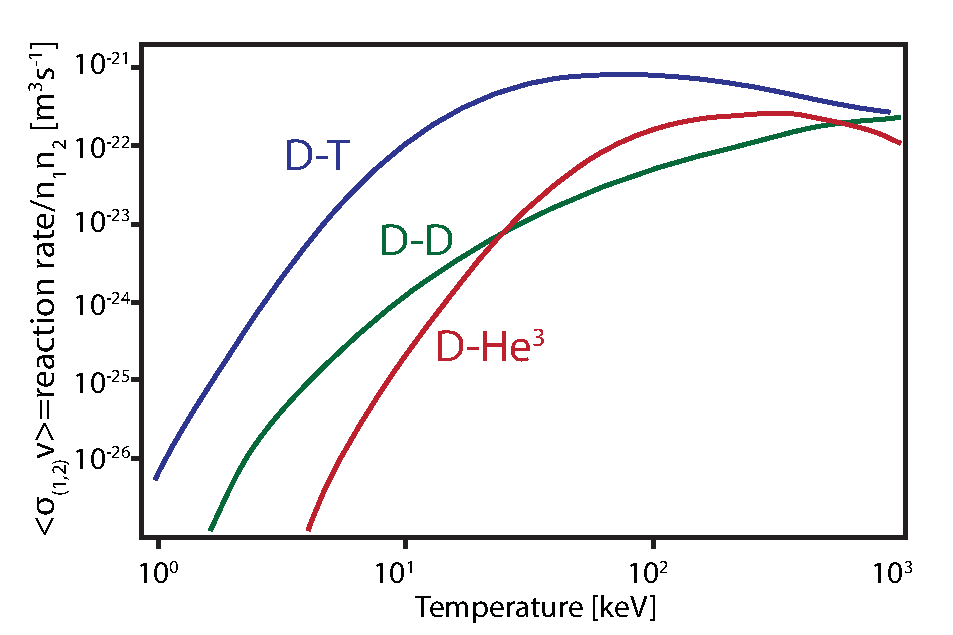
\includegraphics[width=95mm]{graphics/Introduction/reaction_xsections.pdf}}
% \end{figure}

\begin{figure}
 \pushtooutside
 \ffigbox[\FBwidth]{\caption{Binding energy per nucleon versus atomic mass number, with notable isotopes marked.  Reactions forming nuclei with higher binding energy per nucleon are exothermic -- thus, fusion of elements lighter than ${}^{56}\si{Fe}$ or fission of elements heavier than ${}^{56}\si{Fe}$ releases energy.}\label{fig:bindingenergy}}{\includegraphics[width=150mm]{graphics/Introduction/bindingenergy.png}}
\end{figure}

\begin{figure}
 \pushtooutside
 \ffigbox[\FBwidth]{\caption{Reaction rate normalized to fuel density for fusion fuels as a function of temperature.  Notably, deuterium-tritium fusion exhibits a higher peak reaction rate, as well as reaching that peak at a lower temperature, than other fuels.}\label{fig:xsection}}{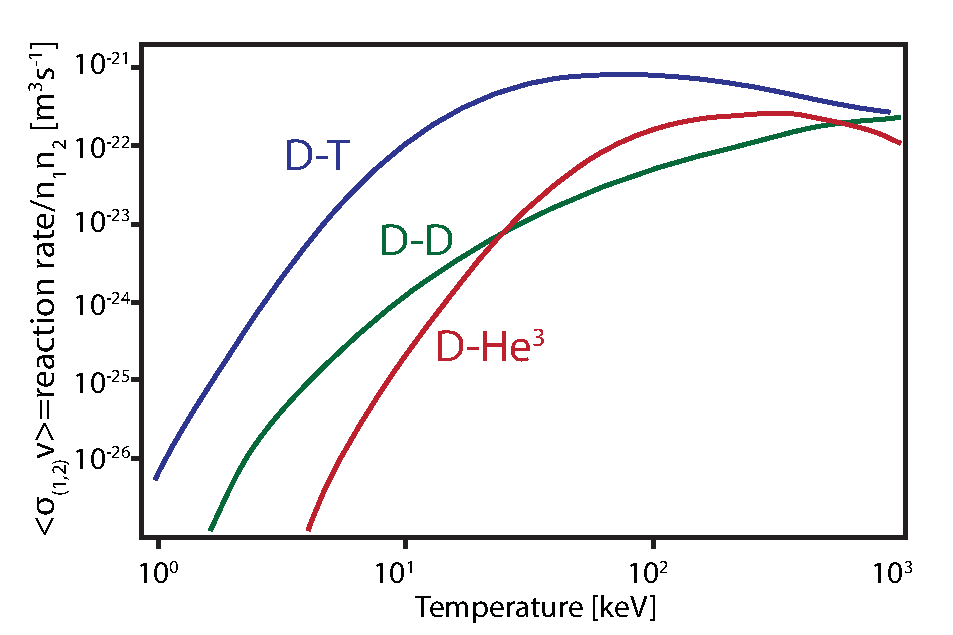
\includegraphics[width=150mm]{graphics/Introduction/reaction_xsections.pdf}}
\end{figure}

Pure deuterium fuel (reactions shown in eqns. \ref{eq:dd1} and \ref{eq:dd2}) is attractive from a research standpoint, due to the abundance and ease of use of deuterium.  Deuterium is a stable nucleus, obviating the need for radiation safety in the fuel system, and is naturally occurring in relative abundance (approximately $1/6000$ of hydrogen nuclei on earth are deuterium \note{cite}), allowing harvesting of deuterium fuel from seawater.  However, pure-deuterium reactions suffer from low energy output per reaction and a significantly lower reaction rate at feasible plasma conditions compared to other fuel options (see Figure~\ref{fig:xsection}), setting high performance requirements for a putative DD-burning reactor.

The $\si{D}-\si{He}^3$ reaction (eqn.~\ref{eq:dhe3}) exhibits several desirable properties, namely an impressive energy yield per reaction, and the fact that the reaction produces only charged particles rather than the high-energy neutrons found in $\si{D}-\si{D}$ and $\si{D}-\si{T}$ reactions, which can cause significant damage to reactor materials.  However, as with $\si{D}-\si{D}$ fuel, the $\si{D}-\si{He}^3$ reaction suffers from a lower reaction rate at attainable conditions, as well as the fact that Helium-3 does not occur in economically usable quantities on Earth.  While off-planet sources of Helium-3 exist (for example, a useful quantity is present in the lunar regolith \note{cite}), this fuel remains the subject of speculation.

The deuterium-tritium reaction (eqn.~\ref{eq:dt}) is considered the most promising for a first-generation fusion reactor, due to its high energy output per reaction and favorable reaction cross-section -- the rate parameter $\langle \sigma v \rangle_{DT}$ reaches its peak at a lower temperature, and reaches a greater absolute level than other fusion fuels.  However, $\si{D}-\si{T}$ operation is limited both by fuel sources, and reaction products.  $\si{D}-\si{T}$ fusion produces a $14 \;\si{MeV}$ neutron, carrying roughly 80\% of the energy released by the fusion reaction, which can damage unshielded reactor materials.  Moreover, while deuterium is stable and readily available, tritium is radioactive with a short half-life (roughly 12.3 years), so it is not naturally occurring in meaningful quantities on earth.   A reactor will solve both of these problems with a \emph{neutron blanket}, a neutron-absorbing structure surrounding the plasma.  This provides the necessary shielding for sensitive reactor components.  The heat generated in the blanket from neutron absorption will also be drawn off in a steam cycle to drive turbines, generating electricity from the reactor.  Finally, seeding the blanket with lithium allows the following reactions with fusion neutrons:

\begin{align}
 {}^6\si{Li} + \si{n}_{slow} &\rightarrow {}^4\si{He} + \si{T} + 4.8 \;\si{MeV}\label{eq:Li6}\\
 {}^7\si{Li} + \si{n}_{fast} &\rightarrow {}^4\si{He} + \si{T} + \si{n} - 8.7 \;\si{MeV}\label{eq:Li7}
\end{align}

\noindent the Lithium-6 reaction (eqn.~\ref{eq:Li6}) absorbs ``slow'' neutrons (that is, neutrons that have thermalized to the blanket temperature via collisions) to produce tritium, plus additional heat.  Lithium-7 (eqn.~\ref{eq:Li7}) is more likely to capture fast neutrons to produce tritium in an endothermic reaction; however, the reaction also acts as a neutron multiplier, as a free neutron is maintained through the reaction.  Using blankets enriched with ${}^6\si{Li}$, coupled with neutron multipliers, a reactor will target an over-unity tritium breeding ratio, with $>1$ tritons produced per neutron entering the blanket (\ie per tritium consumed in a fusion reaction).\nicesectionending

%%%%%%%%%%%%%%%%%%%%%%%%%%%%%%%%%%%%%%%%%%%%%%%%%%%%

\section{Magnetic Confinement}\label{sec:intro_magnetic}

\subsection{Basic Principles}\label{subsec:intro_basic}

\subsection{Toroidal Configurations}\label{subsec:intro_toroidal}

%%%%%%%%%%%%%%%%%%%%%%%%%%%%%%%%%%%%%%%%%%%%%%%%%%%%

\section{Alcator C-Mod}\label{sec:intro_cmod}

%%%%%%%%%%%%%%%%%%%%%%%%%%%%%%%%%%%%%%%%%%%%%%%%%%%%

\section{Confinement \& Transport}\label{sec:intro_confinement}

\subsection{Global Confinement}\label{subsec:intro_global}

\subsection{Transport Barriers}\label{subsec:intro_barriers}

%%%%%%%%%%%%%%%%%%%%%%%%%%%%%%%%%%%%%%%%%%%%%%%%%%%%

\section{High-Performance Regimes}\label{sec:intro_regimes}

\subsection{ELMy H-Mode}\label{subsec:intro_elmy}

\subsection{EDA H-Mode}\label{subsec:intro_EDA}

\subsection{I-Mode}\label{subsec:intro_imode}

%%%%%%%%%%%%%%%%%%%%%%%%%%%%%%%%%%%%%%%%%%%%%%%%%%%%

\section{Goals \& Outline}\label{sec:intro_outline}


%%%%%%%%%%%%%%%%%%%%%%%%%%%%%%%%%%%%%%%%%%%%%%%%%%%%

% do per-chapter bibliographies, or one big one?
%\bibliographystyle{plainurl}
%\bibliography{main} 
\chapter{High-Performance Regimes}\label{ch:HighPerformance}

The development of magnetic-confinement fusion into an economical form of power generation is characterized by two seemingly contrary requirements: first, a high level of energy confinement is necessary to reach the desired level of self-heating of the plasma by fusion products, satisfying triple-product requirements (\cref{eq:tripleproduct}).  At the same time, particle transport must be sufficient to avoid the deleterious effects of accumulated helium ``fusion ash'' and other impurities (particularly high-$Z$ metal wall materials)\gnote{ref why metal walls are necessary?} on fusion performance.

\gnote{introduce pedestal formation, edge rotation}

\begin{table*}[h]
 \pushtooutside
 \ttabbox{\caption{Typical operating parameters of tokamaks noted in this thesis.  \emph{Note:} all ITER values are projected.\note{check all values here, add citations!}}\label{tab:tokamaks}}
 {\begin{tabular}{lccccccc}
  \toprule
  Device &
  $R/a \;[\si{\meter}]$ &
  %$a \;[\si{\meter}]$ &
  $I_p\;[\si{\mega\ampere}]$ &
  $B_T \;[\si{\tesla}]$ &
  $\overline{n}_e \;[\si{\per\meter\cubed}]$ &
  $T_{e0} \;[\si{\kilo\electronvolt}]$ &
  heating &
  refs
  \\
  \midrule
  C-Mod &
  $\num{0.67/0.22}$ &
  %$\num{0.22}$ &
  $\le \num{2}$ &
  $3-8.1$ &
  $\le \num{5e20}$ &
  $\le \num{8}$ &
  ICRF, LHRF &
  \cite{Hutchinson1994}
  \\
  DIII-D &
  $\num{1.67/0.67}$ &
  %$\num{0.67}$ &
  $1-3$ &
  $2.2$ &
  $\num{6e19}$ &
  $5-10$ &
  ECRF, NBI &
  \\
  ASDEX-U &
  $\num{1.65/0.5}$ &
  %$\num{0.5}$ &
  $\sim 1$ &
  $3.9$ &
  $\num{7.5e19}$ &
  $2-3$ &
  &
  \\
  JET &
  $\num{3.4/0.9}$ &
  $3-4$ &
  $3.8$ &
  $\num{5e19}$ &
  $10-20$ &
  &
  \\
  JT-60U &
  $\num{3.4/0.9}$ &
  $3-4$ &
  $4.8$ &
  $\num{5e19}$ &
  $10-20$ &
  &
  \\
  JFT-2M &
  &
  &
  &
  &
  &
  &
  \\
  ITER* &
  &
  &
  &
  &
  &
  &
  \\
  \bottomrule
 \end{tabular}}
\end{table*}

\section{ELM-Free H-Mode}\label{sec:hcr_elmfree}

\nicesectionending

\section{ELMy H-Mode}\label{sec:hcr_elmy}

\subsection{Global Parameters}\label{subsec:hcr_elmy_ped}

\subsection{Fluctuations and ELMs}\label{subsec:hcr_elmy_fluct}

\subsection{Active ELM Control}\label{subsec:hcr_elmy_control}

\nicesectionending

\section{ELM-Suppressed H-Modes}\label{sec:hcr_elmsuppressed}

\subsection{QH-Mode}\label{subsec:hcr_qh}

\subsection{EDA H-Mode}\label{subsec:hcr_eda}

\nicesectionending

\section{I-Mode}\label{sec:hcr_imode}

\subsection{Access and Operation}\label{subsec:hcr_imode_access}

\subsection{Global Performance}\label{subsec:hcr_imode_performance}

\subsection{Edge Fluctuations -- the Weakly-Coherent Mode}\label{subsec:hcr_imode_wcm}

\nicechapterending

\bibliographystyle{../plainurl}
\bibliography{../references}
\chapter{Pedestal Modeling and Theory}\label{ch:Modeling}

While a number of high-performance regimes (described in \cref{ch:HighPerformance}) have been established and are actively explored for tokamak operation, much of the physics governing these regimes is still unknown.  In particular, the physics underlying the structure of the pedestal is an area of active research, due in large part to the inherent difficulty in experimentally diagnosing the pedestal plasma as it varies over short scale lengths, and in the wide variability of H-mode behaviors observed in tokamak experiments.  Nevertheless confidence in the prediction of pedestal height and stability for ITER- and reactor-scale devices is essential: core temperature and pressure in the plasma are strongly sensitive to pedestal conditions due to profile stiffness driven by marginally-stable temperature-gradient modes \cite{Hubbard1998}\gnote{elaborate or reword}, thus fusion power density is controlled by the pressure pedestal structure.  Moreover, operation with large, uncontrolled Edge-Localized Modes (ELMs -- see \cref{sec:hcr_elmy}) can drive transient heat loads exceeding wall material tolerances on ITER-scale devices \cite{Loarte2003,Federici2003} -- an understanding of pedestal stability against ELMs is necessary for ITER operation and beyond.  This chapter provides a review of the efforts to date in theory and modeling of the pedestal, including the theoretical models used in the balance of this thesis.\nicesectionending\gnote{elaborate?}

\section{Early Models}\label{sec:mod_early}

\gnote{needs better title...}Initial efforts in understanding the pedestal took a variety of approaches, including models built from fairly simple \emph{ans\"{a}tze} for the physics determining the pedestal structure.  Several of these approaches are detailed here.  Overviews of these models may also be found in \cite[\S 2]{Hubbard2000,Hughes2005}.

\subsection{Empirical Observations}\label{subsec:mod_empirical}

Absent a firm understanding of the physics underlying the pedestal structure, experimental efforts have sought to characterize the pedestal in terms of simple scalings with engineering parameters.  The pedestal width, in particular, presented significant difficulty in this regard, as it tends to be quite robust, varying only over a narrow range on a given machine \cite{Maggi2010} -- observations on JET \cite{Breger1998} and Alcator C-Mod \cite{Hughes2002,Hughes2007a} found minimal variation of the pedestal width with plasma current or magnetic field, although a somewhat broader pedestal was observed at low current and with strong shaping on C-Mod \cite{Hughes2007,Hughes2007a}.  Accordingly, the measured gradients in density, temperature, and pressure in the steepest region of the pedestal trend linearly with the corresponding value at the pedestal top \cite{Breger1998,Hughes2007a}.

Multivariate dependences on engineering parameters may be explored with a reasonably general approach via power-law scalings, fitting pedestal data to scalings agnostic of any assumed underlying physics.  Suttrop \emph{et al.} \cite{Suttrop1997} found for ASDEX Upgrade pedestals

\begin{equation}
 \nabla p \sim B_T^{-0.31} \; P_{tot}^{0.16} \; \overline{n}_e^{-0.1} \; I_p^{2.1}
\end{equation}

\noindent A similar approach on C-Mod using an extensive dataset of EDA and ELM-free H-modes \cite{Hughes2002} found

\begin{equation}\label{eq:pedfits}
 \begin{aligned}
  n_{e,ped} &\sim I_p^{0.95} \; \overline{n}_{e,L}^{0.39} \; B_T^{-0.46}\\
  T_{e,ped} &\sim I_p^{0.95} \; \overline{n}_{e,L}^{-0.78} \; B_T^{0.80} \; P_{net}^{0.64}\\
  p_{e,ped} &\sim I_p^{1.98} \; \overline{n}_{e,L}^{-0.56} \; P_{net}^{0.48}
 \end{aligned}
\end{equation}

\noindent (here $\overline{n}_{e,L}$ is the L-mode target density, as pedestal density is not readily controllable in EDA H-mode).  However, later studies asserted that the magnetic-field dependence was overstated in the above \cite{Hughes2006}.  While these empirical models perform reasonably well on their respective experimental data, confident extrapolation to ITER-scale operation requires a physics-based understanding of the pedestal structure.

\subsection{Neutral Penetration \& the Density Pedestal}\label{subsec:mod_neutral}

Given the proximity of the plasma pedestal to neutral gas from fueling apparatus and wall outgassing in the edge, it is logical that the density profile should depend strongly on interaction with and ionization of neutral particles in the pedestal.  Based on a relatively simple particle transport model, the pedestal width is expected to scale with the characteristic neutral penetration length before ionization \cite{Hughes2005,Mahdavi2002}:

\begin{equation}\label{eq:neutralpenetration}
 \lambda_{neutral} = \frac{v_n}{n_e \langle \sigma v \rangle_{ion}}
\end{equation}

\noindent where $v_n$ is the velocity of neutrals entering the pedestal (set by the neutral thermal temperature in the edge) and $\langle \sigma v \rangle_{ion}$ is the velocity-averaged ionization cross-section.  Given that $v_n$ is independent of plasma conditions and that $\langle \sigma v \rangle_{ion}$ is consistent over the temperatures of interest in the edge \cite{Hughes2005}, therefore we expect the simple relation $\Delta_{n} \sim 1/n_{e,ped}$.  More complex models for the neutral penetration typically reproduce the dependence on $\lambda_{neutral}$.

However, experimental observations of the density pedestal conflict with these relatively simple predictions.    Observations in similarity experiments between DIII-D, JET, and ASDEX Upgrade \cite{Beurskens2011} were inconsistent with the simple model: although DIII-D data were consistent with the trends found in the model, data from JET were not, and moreover the model predicted an inconsistent scaling between the two machines for pedestal density and width.  Likewise, predictions based on pedestal widths set by neutral penetration performed poorly as a predictor for pedestal height in a multi-machine scaling from AUG, DIII-D, JT-60U, and JET \cite{Onjun2002}.  EDA H-modes on Alcator C-Mod show near-complete insensitivity of the density pedestal to neutral interactions -- the density pedestal instead saturates to a level dictated by plasma transport (predicted best by $n_{e,ped} \sim I_p$), with fueling via edge gas puffing having little effect on the density pedestal \cite{Hughes2006,Hughes2007}.

In addition to significant sensitivity to machine and discharge conditions and wall materials \cite{Beurskens2011}, density pedestal behavior appears to be strongly sensitive to magnetic configuration -- experiments on MAST \cite{Maggi2010} found that, while the density pedestal width was poloidally constant in single-null discharges, the density pedestal is measurably broader on the outboard, low-field side in double-null discharges.  These results indicate that plasma-neutral interactions in the density pedestal are quite complex, and dependent on poloidal transport behaviors and fueling asymmetries \cite{Maggi2010}.  This remains an important area of research, as ITER is expected to have an edge that is highly opaque to neutrals, complicating the density pedestal structure and fueling scenarios for high-density plasmas \cite{Hughes2007,Maggi2010}.

\subsection{Ion-Orbit Loss \& Gyroradius Models}\label{subsec:mod_ionorbitloss}

Due to the importance in the edge $E_r$ well in pedestal formation, modeling efforts naturally turned to potential sources for the electric field to explain the pedestal.  One suggested source was ion orbit loss across the last closed flux surface, in which the gyro-motion of ions near the edge intersect the SOL or the plasma-facing material surfaces -- the charge imbalance induced by this particle ``leak'' results in a radial electric field \cite{Shaing1990}.  Assuming ion orbit losses drive the $E_r$ well, the $\vec{E}\times\vec{B}$ shear layer width ought to be governed by the banana orbit width, which scales as the poloidal gyroradius $\rho_{i,pol} \sim \sqrt{T_i}/B_p$.  Accounting for the squeezing effect of the radial electric field on the banana orbit width, Shaing \cite{Shaing1992} gives for the well width

\begin{equation}\label{eq:Shaing_width}
 \begin{aligned}
  &\Delta_{\vec{E}\times\vec{B}} \propto \sqrt{\varepsilon} \frac{\rho_{i,pol}}{\sqrt{S}}\\
  &S = \left| 1 - \frac{1}{B_p \omega_{ci,p}} \frac{dE_r}{dr}\right|
 \end{aligned}
\end{equation}

\noindent where $S$ is the squeezing factor and $\omega_{ci,p}$ is the ion cyclotron frequency evaluated with the poloidal field.  The model is further refined by Itoh \& Itoh \cite{Itoh1996} to include the broadening effects of viscosity shear.  The predicted trend is observed in ELM-free H-modes on JT-60U \cite{Hatae1998}, with $\Delta \approx 3.3 \sqrt{\varepsilon} \rho_{i,pol}$; however, as the squeezing factor $S$ is estimated to be near-unity, the pedestal width is broader by a factor of $\sim 3.3$ than the $\sim \sqrt{\varepsilon} \rho_{i,pol}$ banana width.  ELMy H-modes on JT-60U exhibit a similar scaling at weak shaping, with a broader pedestal and additional safety factor dependence $\Delta \approx 5 \rho_{i,pol} q_{95}^{-0.3}$ at higher triangularity \cite{Kamada1999}.

However, other predictions and experimental observations contradict these results.  Depending on the calculation method of growth rate suppression by $\vec{E}\times\vec{B}$ sheared flow, the pedestal width may scale with the gyroradius anywhere from $\Delta \sim \left(\rho^*\right)^{1/2}$ to $\Delta \sim \rho^*$, where $\rho^*$ indicates the gyroradius normalized to the plasma minor radius \cite{Onjun2002,Beurskens2011}.  Alternately, stabilization of drift-ballooning modes leads to a predicted dependence of $\Delta \sim \rho_{i,pol}^{2/3}$ \cite{Wilson1997}; similarly, diamagnetic stabilization in the pedestal leads to the prediction of $\Delta \sim I_p^2 \rho_{i,pol}^{2/3}$ \cite{Rogers1999}.  Observations on DIII-D \cite{Osborne1998} found a dependence of $\Delta/R \sim (\rho_{i,pol}/R)^{0.67}$, while observations on ASDEX Upgrade \cite{Beurskens2011,Suttrop2000a} found no gyroradius dependence for the pedestal width.

Distinguishing between these scalings is difficult given the diagnostic complications inherent in pedestal measurements, and the narrow range over which $\rho_i$ or the pedestal and $E_r$ well width vary on a given machine \cite{Gohil1998,Maggi2010}.  Moreover, alternate models propose a scaling with poloidal beta at the pedestal top, rather than poloidal gyroradius, with trends of width of $\Delta \sim \beta_{p,ped}^{0.4}$ to $\sim \beta_{p,ped}^{0.5}$ observed on DIII-D \cite{Osborne1998,Groebner1998a}, JET \cite{Maggi2010}, JT=60U \cite{Urano2008}, and ASDEX Upgrade \cite{Beurskens2011}.  Due to the strong covariance between $\rho_{i,pol} \sim \sqrt{mT}/I_p$ and $\sqrt{\beta_{p,ped}} \sim \sqrt{nT}/I_p$ these trends are quite difficult to separate.  However, dedicated experiments to separate the two, either via pumping to vary density and temperature at fixed pressure, exploiting the density dependence in $\beta_{p,ped}$ \cite{Osborne1998}, or via isotope variation targeting the mass dependence in $\rho_{i,pol}$ \cite{Urano2008,Saibene1999}, found the $\beta_{p,ped}$ scaling to be the better predictor, with a weaker secondary gyroradius dependence $\Delta \sim \rho_{i,pol}^{0.2} \beta_{p,ped}^{0.5}$ \cite{Urano2008,Maggi2010}.  The physics underlying the $\Delta \sim \sqrt{\beta_{p,ped}}$ scaling will be discussed in detail in \cref{sec:mod_turbulence}.\nicesectionending

\section{MHD Stability: Peeling-Ballooning Modes}\label{sec:mod_pb}

Due to the extremely rapid onset of explosive ELM instabilities, ideal MHD modes were identified early on as candidates for the ELM trigger \cite{Wagner1982,Keilhacker1984,Huysmans2005}.  In this section, we detail the development of models for the pedestal structure based on the idea that ELM instabilities represent an ultimate limit on the pedestal.

The stability of a plasma may be assessed via a linear perturbation to the customary MHD equations.  We consider a first-order perturbation $\vec{\xi}$ to a plasma fluid element -- typically the perturbation is considered general in spatial variables, and is taken to be a Fourier harmonic in time, $\vec{\xi} = \vec{\xi}(\psi,\chi,\zeta) \mbox{exp}(i\omega t)$ where $\psi$ is the flux coordinate, $\chi$ is a poloidal angle, and $\zeta$ is a toroidal angle.  Substituting into the first-order perturbation of the MHD equations\gnote{detail these in intro?} results in the simple relation (see \cite[\S 8]{Freidberg1987} for derivation)

\begin{equation}\label{eq:mhd_perturb}
 \rho \frac{d^2 \vec{\xi}}{dt^2} = -\omega^2 \rho \vec{\xi} = \vec{F}\left( \vec{\xi} \right)
\end{equation}

\noindent where $\omega$ is the mode frequency, $\rho$ is the mass density, and $\vec{F}$ is a forcing operator given by

\begin{equation}\label{eq:forcing}
 \begin{aligned}
  \vec{F}\left( \vec{\xi} \right) &= \frac{1}{\mu_0} \left( \nabla \times \vec{B} \right) \times \vec{Q} + \frac{1}{\mu_0} \left( \nabla \times \vec{Q} \right) \times \vec{B} + \nabla \left( \vec{\xi} \cdot \nabla p + \gamma p \nabla \cdot \vec{\xi} \right)\\
  \vec{Q} &= \nabla \times \left( \vec{\xi} \times \vec{B} \right)
 \end{aligned}
\end{equation}

\noindent with $\vec{Q}$ for the perturbed magnetic field and $\gamma$ for the specific heat ratio of the plasma.  The usual treatment of this operator leverages the fact that $\vec{F}$ is self-adjoint (\ie it is its own complex conjugate) -- this permits by integration over the plasma volume $P$ in a variational formulation

\begin{equation}\label{eq:energyprinciple}
 \begin{aligned}
  \omega^2 &= \frac{\delta W \left( \vec{\xi}^*,\vec{\xi} \right)}{K\left(\vec{\xi}^*,\vec{\xi} \right)}\\
  \delta W &= -\frac{1}{2} \int_P \vec{\xi}^* \cdot \vec{F} \left( \vec{\xi} \right) \;d^3 \vec{r}\\
  K &= \frac{1}{2} \int_P \rho \left| \vec{\xi} \right|^2 \;d^3 \vec{r}
 \end{aligned}
\end{equation}

\noindent This formulation permits the use of the \emph{energy principle}: if the potential energy $\delta W$ is negative for any displacement (\ie the perturbation drives the plasma to a more energetically-favorable state) then the mode corresponding to that displacement is unstable, captured by the fact that $\delta W < 0$ requires an imaginary frequency $\omega$ (and thus will have an exponentially growing mode).  

This permits a conceptually straightforward means to assess mode stability.  However, the formulation for $\delta W$ is highly involved (see \cite[\S 8.8]{Freidberg1987}):

\begin{equation}\label{eq:deltaW}
 \begin{aligned}
  \delta W &= \delta W_F + \delta W_S + \delta W_V\\
  \delta W_F &= \frac{1}{2} \int_P d^3 \vec{r} \Bigg[ \frac{|\vec{Q}|^2}{\mu_0} + \frac{B^2}{\mu_0} \left| \nabla \cdot \vec{\xi}_\perp + 2 \vec{\xi}_\perp \cdot \vec{\kappa} \right|^2 + \gamma p \left| \nabla \cdot \vec{\xi} \right|^2\\
  &\quad- 2\left( \vec{\xi}_\perp \cdot \nabla p \right) \left(\vec{\kappa} \cdot \vec{\xi}_\perp^* \right) - j_\parallel \left(\vec{\xi}_\perp^* \times \vec{b} \right) \cdot \vec{Q}_\perp \Bigg]\\
  \delta W_S &= \frac{1}{2} \int_S dS \left| \hat{n} \cdot \vec{\xi}_\perp \right|^2 \hat{n} \cdot \left[ \nabla \left( p + \frac{B^2}{2\mu_0} \right) \right]\\
  \delta W_V &= \frac{1}{2} \int_V d^3 \vec{r} \frac{\left|B_1 \right|^2}{\mu_0}
 \end{aligned}
\end{equation}

\noindent for the fluid, surface, and vacuum energy contributions integrated over the plasma volume $P$, plasma surface $S$, and vacuum volume $V$ respectively (in the above $\vec{\kappa}$ is the vectorized curvature, $\hat{n}$ is the normal vector to the plasma surface, $\vec{b}$ is the background magnetic field unit vector, and $B_1$ is the perturbed magnetic field in the vacuum region).  The complexity of the stability problem necessitates both a firm theoretical understanding to simplify \cref{eq:deltaW} to a tractable form, and numerical approaches to efficiently calculate the stability in experimental plasmas.

\subsection{Ballooning MHD}\label{subsec:mod_balloon}

Examining the fluid energy formulation $\delta W_F$ in \cref{eq:deltaW}, we see two potential sources of instability (that is, negative terms in $\delta W$) -- these identify the pressure gradient $\nabla p$ and the parallel current density $j_\parallel$ as potential sources of free energy to drive unstable modes.  We first consider the pressure-gradient-driven modes, dubbed ``ballooning modes'' for their characteristic perturbation, in which the plasma tends to ``bulge'' outwards due to the pressure gradient.  The mode tends to vary along a field line (with long parallel wavelength, although the most unstable modes have short perpendicular wavelength) such that it is concentrated in regions with the least favorable magnetic curvature, such that the increased stabilizing effect from magnetic field line bending cannot compensate for the destabilizing pressure gradient \cite{Freidberg1987}.  These modes were identified early on as a possible ELM trigger: early experiments in ELMy H-mode observed a limit on the pressure gradient preceding the ELM crash \cite{Kamada1996,Suttrop2000}, with the value of $\nabla p$ at the limit increasing with plasma current and shaping, consistent with ballooning theory (detailed below) \cite{Suttrop2000a}.

Early studies in ballooning modes by Connor, Hastie, and Taylor \cite{Connor1978,Connor1979} focused on the comparatively simple high-$n$ limit.  By minimizing $\delta W$ in terms of displacement parallel to the magnetic field and lying within the flux surface (straightforward due to the slow parallel variation of the ballooning mode), the potential energy may be expressed solely in terms of the displacement normal to the flux surface, $\xi_\psi$ (here expressed for compactness as $X = RB_p \xi_\psi$) in an expansion correct to $O(1/n)$ by

\begin{equation}\label{eq:dW_balloon}
 \begin{aligned}
  \delta W &= \pi \iint d\psi d\chi \Bigg\{ \frac{JB^2}{R^2 B_p^2} \left| k_\parallel X \right|^2 + \frac{R^2 B_p^2}{JB^2} \left| \frac{1}{n} \frac{\partial}{\partial \psi} \left( JB k_\parallel X \right) \right|^2\\
  &\quad- \frac{2J}{B^2} \frac{dp}{d\psi} \left[ \left| X \right|^2 \frac{\partial}{\partial \psi} \left( p + \frac{B^2}{2} \right) - \frac{iF}{JB^2} \frac{\partial}{\partial \chi} \left( \frac{B^2}{2} \right) \frac{X^*}{n} \frac{\partial X}{\partial \psi} \right] \Bigg\}
 \end{aligned}
\end{equation}

\noindent where $J$ is the Jacobian, satisfying $J d\chi = dl/B_p$ for a poloidal arc segment $dl$, $F = RB_T$ encodes the toroidal field (as in the Grad-Shafranov equation, \cref{eq:gradshafranov}) We define the parallel gradient operator $k_\parallel$ such that

\begin{equation}\label{eq:dW_kparallel}
  ik_\parallel = \frac{1}{JB} \left( \frac{\partial}{\partial \chi} + in \nu \right)
\end{equation}

\noindent and $\nu = JB_T/R$ encodes the rotational transform; this requires for rational surfaces that $n \oint \nu d\chi = 2\pi m$ for integer $m,n$.  In \cref{eq:dW_balloon}, the first two terms encode the stabilizing effects of magnetic field line bending; the third defines the destabilizing effect of the pressure gradient, and the fourth contains the effect of curvature, which is stabilizing on the inboard side and destabilizing on the outboard side.  

This is solved using the ``ballooning transform'' formalized in \cite{Connor1978}, which encodes the periodicity of the magnetic shear by a transform from the periodic poloidal angle $\chi$ to an infinite, non-periodic domain $y$ -- the rapid variation in $X$ is then contained in an exponential phase factor $\sim \mbox{exp}(-in\int \nu dy)$, with the mode amplitude in a scale factor $f(\psi,y)$ that is comparatively insensitive to $n$.  The Euler-Lagrange equation minimizing $\delta W$ in \cref{eq:dW_balloon} is satisfied by an equation of the form

\begin{equation}\label{eq:baloo}
 \left( L + \Omega^2 M \right) f = 0
\end{equation}

\noindent where $\Omega^2$ is the eigenvalue of the system and $L,M$ are operators based on the plasma equilibrium and normalized pressure gradient $\alpha_{MHD}$ (see \cref{eq:alphaMHD,eq:alphaMHD_cyl}), with $L$ acting as a differential operator in $y$.  Moreover, the operators are defined as an expansion in orders of $n^{-1/2}$.  To lowest order (appropriate in the $n \rightarrow \infty$ limit) the system reduces to an eigenvalue problem for the local eigenmode characterized by $\omega^2$ \cite{Connor1979}, $(L_0 + \omega^2 M_0)f = 0$ -- in this case, the modes are perfectly localized on their corresponding rational surfaces and decoupled from modes on other surfaces, yielding an exceedingly simple calculation.

Later analyses \cite{Connor1979} included additional terms accounting for the effects of current and current gradient at high $n$, of the form\gnote{signs reversed between Wilson2002, Connor1998a, Connor1979?}

\begin{equation}\label{eq:dW_balloon_current}
  \pi \iint d\psi d\chi \left\{ \frac{X^*}{n} JB k_\parallel \left( \sigma' X \right) - \frac{1}{n} \left[ P^* JB k_\parallel Q + PJBk_\parallel^* Q^* \right] \right\}
\end{equation}

\noindent where

\begin{equation}
 \begin{aligned}
  P &= \sigma X - \frac{B_p^2}{\nu B^2} \frac{F}{n} \frac{\partial}{\partial \psi} \left( JBk_\parallel \right)\\
  Q &= \frac{X}{B^2} \frac{dp}{d\psi} + \frac{F^2}{\nu R^2 B^2} \frac{1}{n} \frac{\partial}{\partial \psi} \left( JBk_\parallel X \right)\\
  \sigma &= \frac{F}{B^2} \frac{dp}{d\psi} + \frac{dF}{d\psi}
 \end{aligned}
\end{equation}

\noindent with the parallel current density contained in $\sigma$.  This does not appreciably modify the solution form in \cref{eq:baloo}, rather defining additional terms in the operators $L$ and $M$ -- to lowest order,

\begin{equation}\label{eq:baloo2}
 \begin{aligned}
  L_0 f &= \frac{\partial}{\partial y} \left\{ \frac{1}{JR^2 B_p^2} \left[ 1 + \left( \frac{R^2 B_p^2}{B} \int^y \frac{d\nu}{d\psi} dy \right)^2 \right] \frac{\partial f}{\partial y} \right\}\\
  &\qquad + f \left\{ \frac{2J}{B^2} \frac{dp}{d\psi} \frac{\partial}{\partial \psi} \left( p + \frac{B^2}{2} \right) - \frac{F}{B^4} \frac{dp}{d\psi} \left( \int^y \frac{d\nu}{d\psi} dy \right) \frac{\partial B^2}{\partial y} \right\}\\
  M_0 f &= \frac{J}{R^2 B_p^2} \left[ 1 + \left( \frac{R^2 B_p^2}{B} \int^y \frac{d\nu}{d\psi} \right)^2 \right] f
 \end{aligned}
\end{equation}

\noindent This form is used in the current implementation of the BALOO code \cite{Connor1979,Miller1987,Miller1997}, which efficiently calculates the infinite-$n$ ballooning stability limit.

\begin{itemize}
 \item measured $\alpha_{MHD}$ exceeds stable prediction by BALOO in DIII-D ELMy H-modes -- need to account for current, finite-$n$ effects \cite{Groebner1998a,Osborne1998}
 \item EDA H-mode modeled to be ideal-ballooning stable; P-B only describes ELMy H-mode \cite{Mossessian2002}
 \item increased triangularity reduces $\nabla p$, $n_{e,ped}$ in EDA; contrast with ELMy, where shape stabilizes P-B modes, seems to destabilize QCM earlier in EDA \cite{Hughes2007a}
 \item DIII-D VH-modes terminate in giant p-b driven ELM \cite{Turnbull2003}
\end{itemize}

\subsection{Peeling MHD}\label{subsec:mod_peel}

\subsection{ELITE Code}\label{subsec:mod_elite}

\begin{itemize}
 \item strong shaping impacts stability contour in $j-\alpha_{MHD}$ space \cite{Snyder2009}
 \item collisionality $\rightarrow$ bootstrap current $\rightarrow$ magnetic shear in edge sets where in stability contour pedestal hits \cite{Snyder2009}
 \item due to interplay, nonlocal effects between shaping, collisionality, rotation, shafranov shift, safety factor, must calculate P-B stability in 2D: can't reduce to scalar parametrization \cite{Snyder2009}
 \item Snyder2009 refs Huysmans2005, Turnbull2003, Medvedev2006 \cite{Huysmans2005,Turnbull2003,Medvedev2006} for reviews of alternate MHD codes
 \item alternate MHD codes: GATO \cite{Bernard1981}, MISHKA \cite{Huysmans2001,Mikhailovskii1997}, KINX \cite{Degtyarev1997,Medvedev2006}, MARG2D \cite{Aiba2006,Aiba2007}
 \item RMP approaches P-B boundary, EDA, type-III ELMs P-B stable, grassy/type-II ELMs near boundary, QH near low-$n$ peeling side -- P-B boundary figure of merit in general for H-mode pedestal \cite{Snyder2009}.  RMP calcs stable, goes ELMing and crosses boundary as soon as coils are turned off \cite{Snyder2009a}
 \item very low $n$ ($n < 3$) modes omitted from ELITE: low-$n$ edge modes rarely more unstable than $n \sim 5$, code cannot distinguish from core kink modes, low-$n$ modes stabilized by interaction with wall \cite{Snyder2009}
 \item ELITE omits X-point from calculation due to required extremely high RZ point density; peeling modes highly unstable there, but high collisionality at LCFS suppresses.  Calculation usually truncated at 99.8\% flux \cite{Snyder2009a}
 \item check Snyder2009a for ELITE alternate refs; Huysmans2005, Wilson2006 for reviews \cite{Snyder2009a,Huysmans2005,Wilson2006}
\end{itemize}

\begin{figure}
 \pushtooutside
 \ffigbox[\FBwidth]{\includegraphics[width=150mm]{graphics/ModelingTheory/pb_modestructure.pdf}}{\caption[Mode structure for $n=30$ model calculated by ELITE.]{Mode structure for an $n=30$ ballooning mode calculated by ELITE.  (left) Contour plot of radial perturbations from the mode.  The mode is edge-localized and strongest at the outboard midplane, consistent with an edge ballooning mode.  (right) Eigenmode structure of the $n=30$ mode.  Each peak is a poloidal harmonic localized around the rational flux surface determined by the corresponding poloidal mode number $m$ for $n=30$.  The mode is strongest in the steep gradient region, but extends inward due to the comparatively high mode number (eigenmode envelope encompasses $O(n^{1/3})$ flux surfaces).  Note that, as ELITE cannot treat the separatrix, the mode calculation truncates at $\psi_{norm} = 0.995$.}\label{fig:pb_modestructure}}
\end{figure}

\begin{figure}
 \pushtooutside
 \fcapside[60mm]{\caption[Schematic of peeling-ballooning MHD stability space.]{Schematic of the stability space to coupled peeling-ballooning MHD modes, set by the edge pressure gradient and current density.  Ballooning modes are driven by pressure gradient but stabilized by magnetic shear driven by edge currents, while kink/peeling modes are current-driven but stabilized by pressure gradients.  \note{Ref to Snyder?}}\label{fig:mod_pbcartoon}}{\includegraphics[width=100mm]{graphics/ModelingTheory/pbcartoon.pdf}}
\end{figure}

\begin{figure}
 \pushtooutside
 \fcapside[60mm]{\caption[ELITE calculation of P-B stability in a C-Mod ELMy H-mode.]{Calculation of the peeling-ballooning MHD stability contour from ELITE for an ELMy H-mode pedestal on C-Mod.  To within error bars, the pedestal lies on the peeling-ballooning boundary.  The comparatively higher collisionality typical of C-Mod H-mode pedestals pushes the MHD behavior of the pedestal towards higher-$n$, pure-ballooning modes, although moderate-$n$ coupled modes in the ``nose'' of the stability contour are also common.}\label{fig:mod_elmy_elite}}{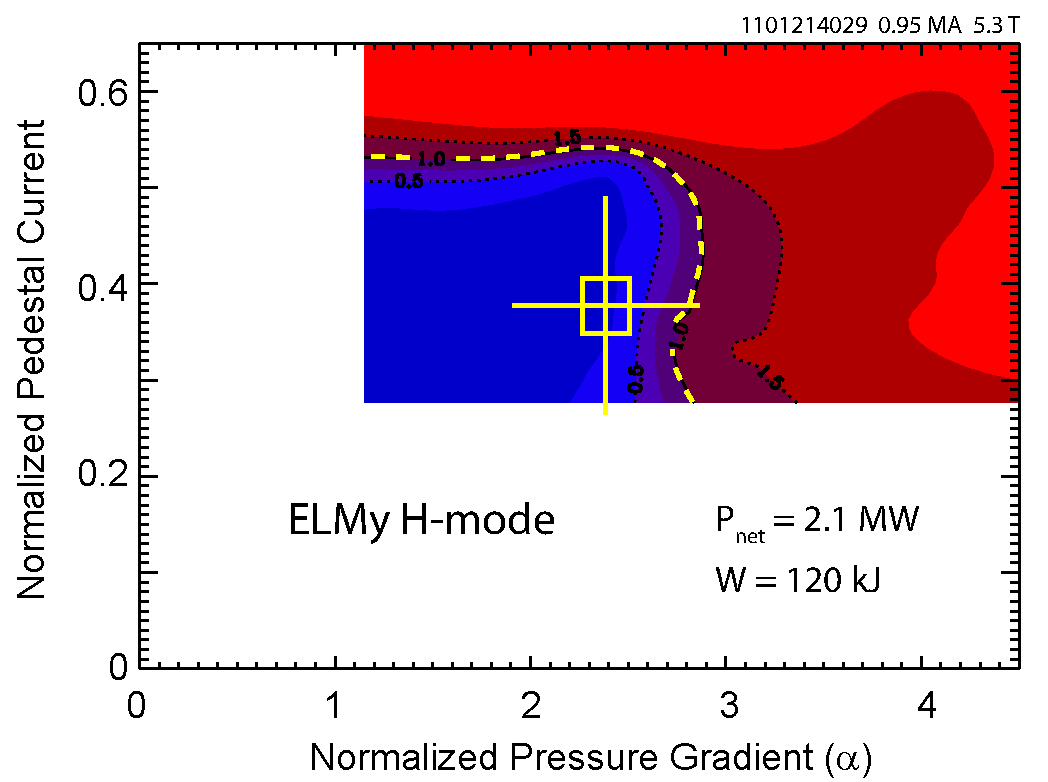
\includegraphics[width=100mm]{graphics/ModelingTheory/elmy_elite_nobal.pdf}}
\end{figure}

\nicesectionending

\section{Kinetic-Ballooning Turbulence Modeling}\label{sec:mod_turbulence}

\begin{itemize}
 \item after L-H transition, $\vec{E}\times\vec{B}$ flows continue to rise due to increased diamagnetic term $\rightarrow$ suppresses long-wavelength drift wave turbulence, drift-alfven waves.  Need short wavelength mode to limit pedestal growth. \cite{Snyder2009}
 \item ETG more likely to modify density vs. temperature, rather than limit pressure; instead consider kinetic ballooning mode \cite{Snyder2009}
 \item Snyder2009 refs Snyder thesis, Jenko2001, Scott2003, Candy2005 \cite{Snyder1999,Jenko2001,Scott2003,Candy2005}, Snyder2010 refs thesis, Jenko, Candy, add Snyder2001 \cite{Snyder2001}
 \item KBM threshold correlated to high-$n$ ideal ballooning MHD, reduced due to dissipative, ion-drift resonance effects \cite{Snyder2009}
 \item KBM onset largely independent of $\vec{E} \times \vec{B}$ shear, linear onset at $\alpha_{crit}$ \cite{Snyder2009}
 \item scaling: $\langle \alpha_c \rangle \sim \beta_{p,ped} / \Delta \rightarrow \Delta \sim \beta_{p,ped}/\langle \alpha_c \rangle$.  gradient stabilized by magnetic shear, so $\langle \alpha_c \rangle \sim 1/s^{1/2}$; $s \sim 1/j \sim 1/\beta_{p,ped} \rightarrow \alpha_c \sim \beta_{p,ped}^{1/2} \rightarrow \Delta \sim \beta_{p,ped}^{1/2}$ \cite{Snyder2009}
 \item $\beta_{p,ped}$ width scaling seen experimentally on DIII-D \cite{Osborne1998,Groebner2013}, JT-60U \cite{Oyama2005,Urano2008}, AUG \cite{Gruber1999,Beurskens2011}, C-Mod \cite{LaBombard2008,Walk2012}
 \item increased global $\beta$ increases MHD stability, but not enough to explain increased pedestal - wider pedestal with more $\beta_{p,ped}$ does explain \cite{Snyder2009a}
 \item pedestal grows maintaining $\Delta \sim \beta_{p,ped}^{1/2}$ -- KBM saturates early \cite{Maggi2010,Hughes2013}
 \item fluctuation observations of early saturation of KBM \cite{Diallo2014}
\end{itemize}

\noindent\note{BCP description!!!}

\subsection{The Ballooning-Critical Pedestal Technique}\label{subsec:mod_bcp}

The KBM is an approximately local effect due to its short scale length -- as such, no single calculated mode can describe the destabilization of the entire pedestal without a highly involved nonlocal calculation of the stability across the pedestal profile.  A far more efficient and straightforward model can be developed using the ``ballooning critical pedestal'' (BCP) technique \cite{Snyder2010,Snyder2011}, which finds the point where half of the pedestal is locally at or beyond criticality for the KBM.  At fixed pedestal width, the height is incremented to increase the pressure gradient, following the same approach as the peeling-ballooning calculation.  At each increment, the stability of the pedestal to high-$n$ ideal ballooning MHD modes is calculated, \eg using the BALOO code \cite{Connor1979,Miller1987}.  As the infinite-$n$ modes calculated by BALOO are also perfectly localized on the corresponding rational flux surfaces\gnote{explain?}, the code finds unstable surfaces in the pedestal region and the width of the pedestal covered by these surfaces.  When half of the pedestal width is thus unstable, the KBM threshold is said to have been reached.  This approach is highly numerically efficient -- as the ballooning MHD criterion reduces in the infinite-$n$ limit to a straightforward one-dimensional eigenvalue problem \cite{Connor1979} that can be computed efficiently -- and fairly robust, although it does require the unstable region of the pedestal to be well-defined and bounded (typically the ``middle half'' of the pedestal, where the pressure gradient is steepest).  This assumption can break down at very strong shaping or low aspect ratio \cite{Snyder2011}.\nicesectionending

\section{The EPED Model}\label{sec:mod_eped}

In light of the importance of the pedestal structure for optimized fusion performance -- both by maximizing fusion power density via the pressure pedestal height constraint on core profiles \cite{Kinsey2011}, and by avoiding or mitigating large, damaging ELMs \cite{Loarte2003,Federici2003} -- a predictive understanding of the pedestal is highly desirable for planned operations on ITER and beyond.  Models based on peeling-ballooning MHD instability, particularly the ELITE code (\cref{subsec:mod_elite}), have proven quite successful at capturing the limiting physics of the ELMy H-mode pedestal.  However, these calculations typically rely on experimental profiles and magnetic equilibria reconstructed after the fact, and as such cannot by themselves provide predictive capability.  Similarly, the constraint set by kinetic-ballooning mode (KBM) turbulence (\cref{sec:mod_turbulence}) corresponds well with pedestal observations in profiles with steep pressure gradients in the pedestal, but cannot by itself uniquely constrain the pedestal structure.  Here we introduce the EPED series of models \cite{Snyder2011}, which combines these two constraints into a single predictive model for the ELMy H-mode pedestal.

To incorporate predictive capability into the peeling-ballooning MHD stability model calculated by ELITE, the EPED model must characterize peeling-ballooning stability as accurately as possible using only parameters known prior to the plasma discharge, set by operator control; however, as discussed in \cref{subsec:mod_elite}, the inherent nonlocality of the problem still requires a 2-dimensional MHD calculation.  To that end, the model employs a set of model Miller equilibria \cite{Miller1998}, up/down-symmetric equilibria allowing for plasma elongation and triangularity defined with analytic plasma profiles such that the essential physics in the pedestal (namely, the pressure gradient and bootstrap current profiles) is nearly matched to experimental conditions \cite{Snyder2009}.  Using this setup, the model equilibria may be defined by a small set of scalar parameters for use in ELITE: major and minor radius $R$ and $a$, elongation and shaping $\kappa$, $\delta$ (recall that in these up/down-symmetric equilibria $\delta_l = \delta_u = \delta$), plasma current $I_p$, and applied field $B_T$, set the magnetic equilibrium when combined with the target global normalized pressure (typically the Troyon normalized $\beta_N$ \cite{Troyon1984}).  Global beta also impacts the pedestal stability via the beneficial effect of increased Shafranov shift in the core on MHD stability\gnote{ref this in peeling-ballooning section!}.  The model additionally takes as inputs the density at the pedestal top $n_{e,ped}$ and the pedestal width $\Delta$ in normalized poloidal flux (note that the density and temperature profiles are defined to have the same width) to constrain the pressure and current profiles, with the current calculated from the density and temperature profiles from the analytic Sauter formula, \cref{eq:jboot} \cite{Sauter1999}.

The calculation of the peeling-ballooning stability boundary is straightforward -- at a fixed pedestal width, the pressure pedestal height (and, accordingly, the MHD instability drives from the edge pressure gradient and current density) is increased in increments until the stability boundary is reached \cite{Snyder2009}.  The interdependence between pedestal width and height is determined by repeating the calculation at a range of pedestal widths, determining a relation between the pressure pedestal width and height for a given model equilibrium.  To lowest order, the MHD limit is a limit on $\nabla p$, leading one to expect a linear relation between the pedestal width and height.  However, nonlocal effects on the MHD stability -- in particular, the broader, lower-$n$ modes destabilized by wider pedestals leading to reduced maximum $\alpha_{MHD}$ at wider $\Delta$ -- reduces the linear dependence, leading to a rough scaling of $p_{ped} \sim \Delta^{3/4}$ set by the peeling-ballooning stability boundary \
cite{Snyder2009a}.

On its own, the peeling-ballooning MHD constraint defines the pedestal height as a function of width, necessitating a second constraint to allow a unique predictive solution.  The Kinetic Ballooning Mode (KBM), described in \cref{sec:mod_turbulence}, limits the pedestal gradient with a relation $p_{ped} \sim \Delta^2$ (more precisely, $\Delta \sim \beta_{p,ped}^{1/2}$).  This constraint is sufficiently distinct from that enforced by peeling-ballooning MHD  that only a single nontrivial solution satisfying both exists -- thereby uniquely predicting the pedestal width and height.  An example of the prediction at the intersection of the P-B and KBM constraints, along with the corresponding experimental result \cite{Snyder2011}, is shown in \cref{fig:mod_epedcartoon}.

\begin{figure}[ht]
 \pushtooutside
 \fcapside[60mm]{\caption[Illustration of the peeling-ballooning MHD and KBM constraints used in the EPED model.]{Illustration of the peeling-ballooning MHD and kinetic-ballooning turbulent constraints used in the EPED model.  The peeling-ballooning constraint, calculated by ELITE, results in a trend roughly of $p_{ped} \sim \Delta_\psi^{3/4}$, while the KBM width constraint calculated via the ballooning-critical pedestal (BCP) technique sets $p_{ped} \sim \Delta_\psi^{2}$.  The unique solution to these constraints is the EPED prediction for the pedestal width and height.  The prediction is here shown compared to the measured pedestal from DIII-D shot 132003 (reproduced from \cite{Snyder2011}) \note{get permission}}\label{fig:mod_epedcartoon}}{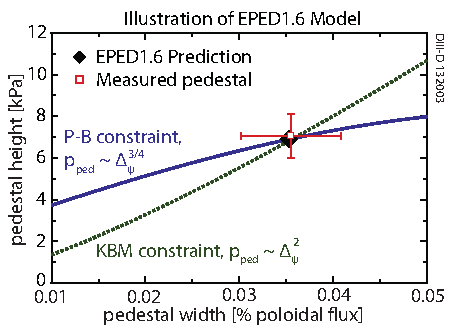
\includegraphics[width=100mm]{graphics/ModelingTheory/epedcartoon.pdf}}
\end{figure}

\subsection{EPED1}\label{subsec:mod_eped1}

The simplest version of the EPED series, EPED1 \cite{Snyder2009}, takes advantage of the dominant scaling of the width with $\beta_{p,ped}$ in the KBM constraint: as little secondary variation of the width beyond $\Delta \sim \beta_{p,ped}^{1/2}$ is seen with other expected controlling parameters, \eg $\nu^*$, $\rho^*$ or $\rho^*_{pol}$, $n_{e,ped}$ \cite{Snyder2009} (\cf \cref{sec:mod_early}, particularly \cref{subsec:mod_ionorbitloss}), the constraint is reduced to a single relation $\Delta = c \beta_{p,ped}^{1/2}$ with a fitted value for $c$.  For historical reasons based on DIII-D data, EPED1 uses $c = 0.076$, although a newer multi-machine fit produces $c = 0.084$ \cite{Snyder2011}. 

To calculate the threshold for the peeling-ballooning MHD instability, the growth rate as calculated by ELITE must be balanced against against the inherent stabilizing effect of plasma diamagnetism in the pedestal\gnote{ref or elaboration on this, or mention in ELITE section?}.  In the EPED1 model this effect is taken to be the solution to $\gamma_{MHD} = \omega (\omega - \omega_{*pi})$, where $\gamma_{MHD}$ is the instability growth rate and $\omega_{*pi}$ is the half-maximum diamagnetic frequency in the pedestal \cite{Snyder2009}.  This leads to a threshold for the growth rate of $\gamma_{MHD} > \omega_{*pi}/2$ for the peeling-ballooning onset\gnote{refs are remarkably reticent to define $\omega_{*pi}$}.  Despite this simple treatment of the KBM and P-B constraints, the EPED1 model is capable of producing predictions with a systematic $\pm 15-20\%$ uncertainty across a range of parameters \cite{Snyder2009,Snyder2010}.

\subsection{EPED1.6}\label{subsec:mod_eped16}

Although the bulk of the variation in the KBM-constrained pedestal width is captured by the $\beta_{p,ped}$ scaling, it is nevertheless desirable to account for its effects on the scale factor of the trend -- more properly, the weakly-varying function $G(\nu^*,\varepsilon,...)$ such that $\Delta = G \beta_{p,ped}^{1/2}$ -- allowing EPED to make first-principles predictions (in that the constraint is not dependent on a scale factor set by fitted data).  

The EPED1.6 implementation \cite{Snyder2010,Snyder2011} achieves this by directly calculating the KBM constraint via the ``ballooning critical pedestal'' (BCP) technique, described in \cref{subsec:mod_bcp}.    By performing this calculation across a range of pedestal widths and fitting the result against $\beta_{p,ped}$, a first-principles calculation of the KBM pedestal constraint is generated and paired with the peeling-ballooning MHD result \cite{Snyder2011}.  While this approach is more computationally expensive than the fixed scaling used in EPED1, the BCP calculation allows the effects of collisionality and shaping on the KBM threshold to be properly accounted for -- this manifests in a range of scale factors, $\langle G \rangle \approx 0.07-0.1$, that are comparable to the fitted result used in EPED1, but are specific to discharge characteristics.

The simple diamagnetic stabilization model used in EPED1, $\gamma_{MHD} > \omega_{*pi}/2$, also fails to capture important physics in the pedestal -- the model assumes a constant diamagnetic frequency $\omega_{*pi}$ for the stabilization of the peeling-ballooning modes, while in fact the diamagnetic frequency varies rapidly over the pedestal \cite{Snyder2010}.  EPED1.6 replaces this with an ``effective'' diamagnetic frequency $\omega_{*eff}$, determined by directly calculating the diamagnetic stabilization of peeling-ballooning modes in the fluid code BOUT++ \cite{Xu2010,Xia2013}.  This provides stronger stabilization of higher-$n$ ($n > \sim 12$) modes at higher collisionality than that found in the simple linear model \cite{Snyder2011,Hughes2013}, a correction that is particularly necessary for the comparatively high-collisionality pedestals in ELMy H-modes on C-Mod \cite{Hughes2013}.

\subsection{EPED Model Implementation \& ITER Predictions}\label{subsec:mod_eped_iter}

The EPED model has been extensively tested on numerous machines, particularly on DIII-D \cite{Snyder2011,Groebner2013}, JT-60U \cite{Snyder2009a}, C-Mod \cite{Walk2012}, and KSTAR \cite{Han2013}.  The model has also been tested on NSTX \cite{Groebner2013}, with limited success due to breakdown of the assumptions inherent to the KBM constraint at small aspect ratio \cite{Snyder2009a}.  Given the proximity of the pedestal to the peeling-ballooning MHD and KBM turbulence limits in most high-performance regimes, it is expected that EPED predictions are viable as a figure of merit for H-mode operation on ITER \cite{Snyder2011,Snyder2012}.

\begin{figure}[ht]
 \pushtooutside
 \fcapside[60mm]{\caption[EPED predictions versus measured pressure pedestal heights.]{EPED predictions versus measured pressure pedestal heights from DIII-D and C-Mod, spanning a significant range of pedestal pressures.  Notably, C-Mod pressure pedestals reach within a factor of $\sim 2$ of the predicted ITER pedestal height.  Reproduced from \cite{Hughes2013} \note{permission!}}\label{fig:mod_epedpredictions}}{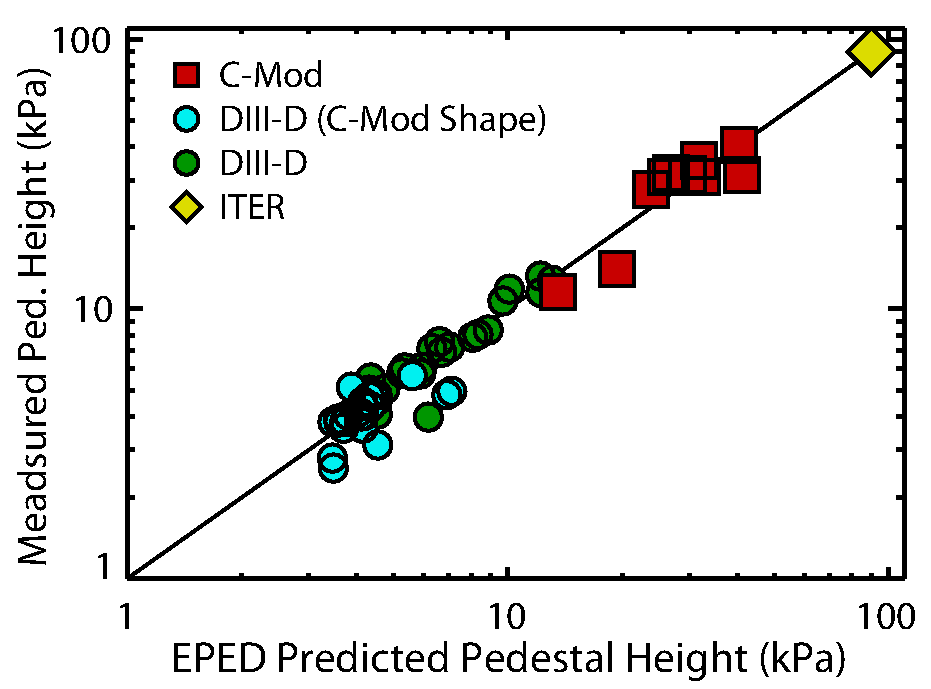
\includegraphics[width=100mm]{graphics/ModelingTheory/eped.pdf}}
\end{figure}

\noindent Notably, EPED predictions for ITER (shown compared to results from DIII-D and C-Mod \cite{Hughes2013} in \cref{fig:mod_epedpredictions}) predict pedestal pressures of $\beta_{N,ped} \sim 0.6-0.7$, corresponding to $p_{ped} \sim \SI{90}{\kilo\pascal}$, at a pedestal width of $\Delta \sim 4\%$ \cite{Snyder2009a,Snyder2011}.  This is within a factor of $\sim 2-3$ of the range of experimental results on which EPED has been tested \cite{Walk2012,Hughes2013}, and is consistent with the planned $Q=10$ operation on ITER assuming sufficient optimization of core and pedestal profiles \cite{Snyder2011,Snyder2012}.  Although development is ongoing for the EPED model series, it has demonstrated viable predictive capability for H-mode pedestals in a variety of conditions for conventional-aspect-ratio tokamaks.\nicechapterending

\bibliographystyle{../plainurl}
\bibliography{../references}
\chapter{ELMy H-Modes on C-Mod}\label{ch:Elmy}

The ELMy H-mode \cite{Wagner1982,Keilhacker1984}, described in \cref{sec:hcr_elmy}, is the most commonly-accessed high-performance regime on major tokamak experiments.  The bursty transport driven by ELMs provides sufficient relaxation of the particle confinement in H-mode to allow stationary operation without excessive impurity accumulation; as such, the ELMy H-mode is considered the baseline operating regime for ITER \cite{ITER1999,Shimada2007}.  However, on ITER-scale devices the pulsed heat loading associated with ELMs drives unacceptable levels of erosion and damage to plasma-facing wall and divertor materials \cite{Loarte2003,Federici2003}.

In light of the impact of large, deleterious ELMs on the ITER wall, and the profound impact of pedestal height on overall plasma performance \cite{Kinsey2011,Doyle2007}, a firm understanding of the physics governing the pedestal in high-performance regimes and their extrapolation to reactor-scale devices is of paramount importance to fusion research leading up to ITER operation.  To that end, a Joint Research Target combining theory, experiment, and modeling efforts in the ELMy H-mode pedestal was undertaken \cite{Groebner2013}\gnote{cite tech report too?}.  Notably, this effort saw the development of the EPED model \cite{Snyder2009,Snyder2011,Snyder2009a}, described in \cref{sec:mod_eped}, which predicts the pressure pedestal width and height preceding the ELM crash through a combination of constraints based on peeling-ballooning MHD instability \cite{Snyder2004,Wilson2002,Wilson2006} (\cref{sec:mod_pb}) and kinetic-ballooning turbulence \cite{Snyder2001} (\cref{sec:mod_turbulence}).  In this chapter, we detail the contributions from Alcator C-Mod to this joint effort \cite{Walk2012}\gnote{how to emphasize my own contribution?} both in empirical studies of the ELMy H-mode pedestal, and in the implementation of the EPED model.  C-Mod ELMy H-modes greatly expand the parameter space in which the EPED model is tested, reaching within a factor of two of the target pedestal pressure for ITER.  The techniques developed in this analysis will subsequently be applied to I-mode pedestals\gnote{reword}.\nicesectionending

\section{ELMy H-Mode Access \& Experimental Arrangement}\label{sec:elmy_access}

\begin{figure}[t]
 \pushtooutside
 \fcapside[55mm]{\caption{C-Mod cross-section comparing the typical plasma shape (blue) to the altered shape favoring ELMy H-mode operation (red), developed in joint experiments with the JFT-2M tokamak \cite{Hughes2013}.  ELMy H-mode access is favored by high lower triangularity and an outer strike point in the divertor slot, coupled with very low upper triangularity and elongation.  This is thought to reduce the required edge pressure gradient and current to reach the peeling-ballooning boundary.}\label{fig:elmy_shaping}}{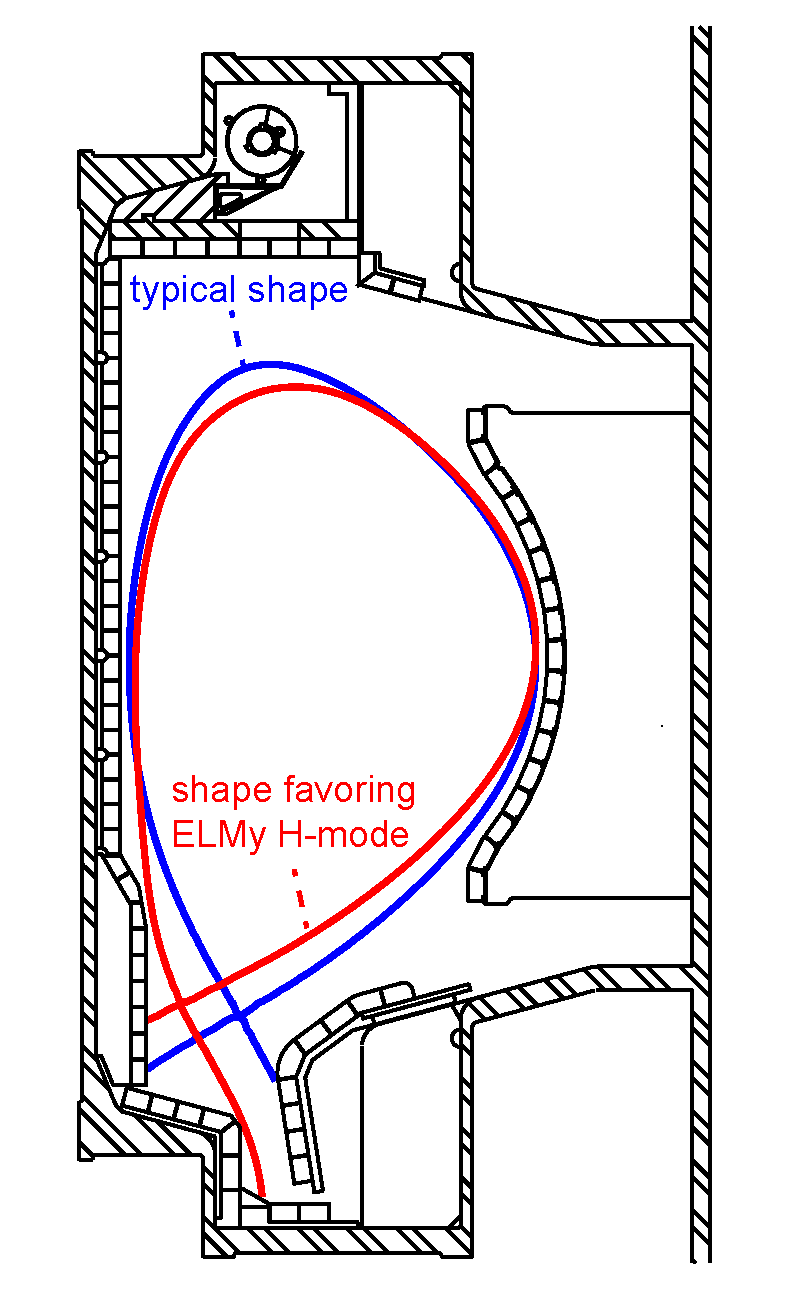
\includegraphics[width=90mm]{graphics/ELMy/shaping.pdf}}
\end{figure}

High-confinement operation on Alcator C-Mod differs is unique among major tokamak experiments in that typical H-modes do not exhibit the large Type-I ELMs\gnote{cite for this?} customarily seen on other devices.  Instead, ELM-free H-modes tend to form at lower collisionalities heating power levels, with high-density, high-power operation tending towards the continuously-regulated EDA H-mode rather than exhibiting discrete ELMs (see \cref{sec:hcr_elmfree,subsec:hcr_eda}).  However, by operating in a modified shape (see \cref{fig:elmy_shaping})\gnote{shape range} with low elongation and upper triangularity paired with high lower triangularity and a strike point on the divertor floor, regular ELMy H-mode operation is attainable.  This comparatively weak shaping, developed in similarity experiments with the JFT-2M tokamak \cite{Hughes2011}\gnote{better cite, Terry paper?}, reduces the necessary pressure gradient and bootstrap current to reach the ideal peeling-ballooning MHD stability boundary (described in \cref{sec:mod_pb}), triggering the ELM.  In this shape, new experiments on C-Mod \cite{Walk2012} attained ELMy H-modes across a broad range in current ($400-1100 \;\si{\kilo\ampere}$) and field ($3.5-8 \;\si{\tesla}$) with high-resolution pedestal data.

\begin{figure}[t]
 \pushtooutside
 \ffigbox[\FBwidth]{
\includegraphics[width=150mm]{graphics/ELMy/time_window.pdf}}{\caption{Example ELMy H-mode window (highlighted).  Phases for study are selected for steady density ($\overline{n}_e$ shown in the top trace), temperature (ECE $T_e$ signals shown for the core and pedestal), and ELM cycles ($D_\alpha$ signal shown).  The same modeling window is shown zoomed-in at the right.  Note the strong perturbation to the edge temperature due to the sawtooth crash.  Thomson scattering frames are indicated by the black ticks on the axes -- the ELM cycle is at a comparable frequency, $\sim \SI{60}{\hertz}$, to the TS system frame rate.  This presents a difficulty for selecting data masked to the ``peak'' of the ELM cycle, necessitating long, steady ELMing phases for study.}\label{fig:elmy_timewindow}}
\end{figure}

Pedestal profiles are taken with the edge Thomson scattering system, detailed in \cref{subsec:app_ts_cmod}.  The pedestal data is taken over steady ELMing phases to minimize the effects of random scatter in the data -- an example of such a window, with line-averaged density $\overline{n}_e$, core and edge $T_e$, and divertor $D_\alpha$ signal (indicative of the ELM crash), is shown in \cref{fig:elmy_timewindow}.  Strictly, models of the pedestal structure in ELMy H-mode predict the pedestal immediately preceding the ELM crash, when the pedestal is most unstable to the ELM trigger.  However, ELMs on C-Mod typically cycle at $60-100 \;\si{\hertz}$, comparable to the repetition rate of the Thomson scattering system (as shown in \cref{fig:elmy_timewindow}).  This presents difficulties in resolving the pedestal with multiple frames per ELM and binning the data to the peaks of the ELM cycle.  In most cases, pedestals are prepared in a single ``ensemble average'' utilizing all TS data in the window; in certain cases, a statistical set is also constructed using the last 20\% of the ELM cycle as is typical for other machines.  The results from this correction are discussed in \cref{sec:elmy_sync}.

\begin{figure}
 \pushtooutside
 \fcapside[65mm]{\caption{Example pedestal illustrating the $mtanh$ function used for pedestal fitting, defining the parameters: height $h$, baseline $b$, midpoint $x_0$, half-width $\delta$/full width $\Delta$.  The inboard slope is characterized by the parameter $\alpha$.}\label{fig:mtanh}}{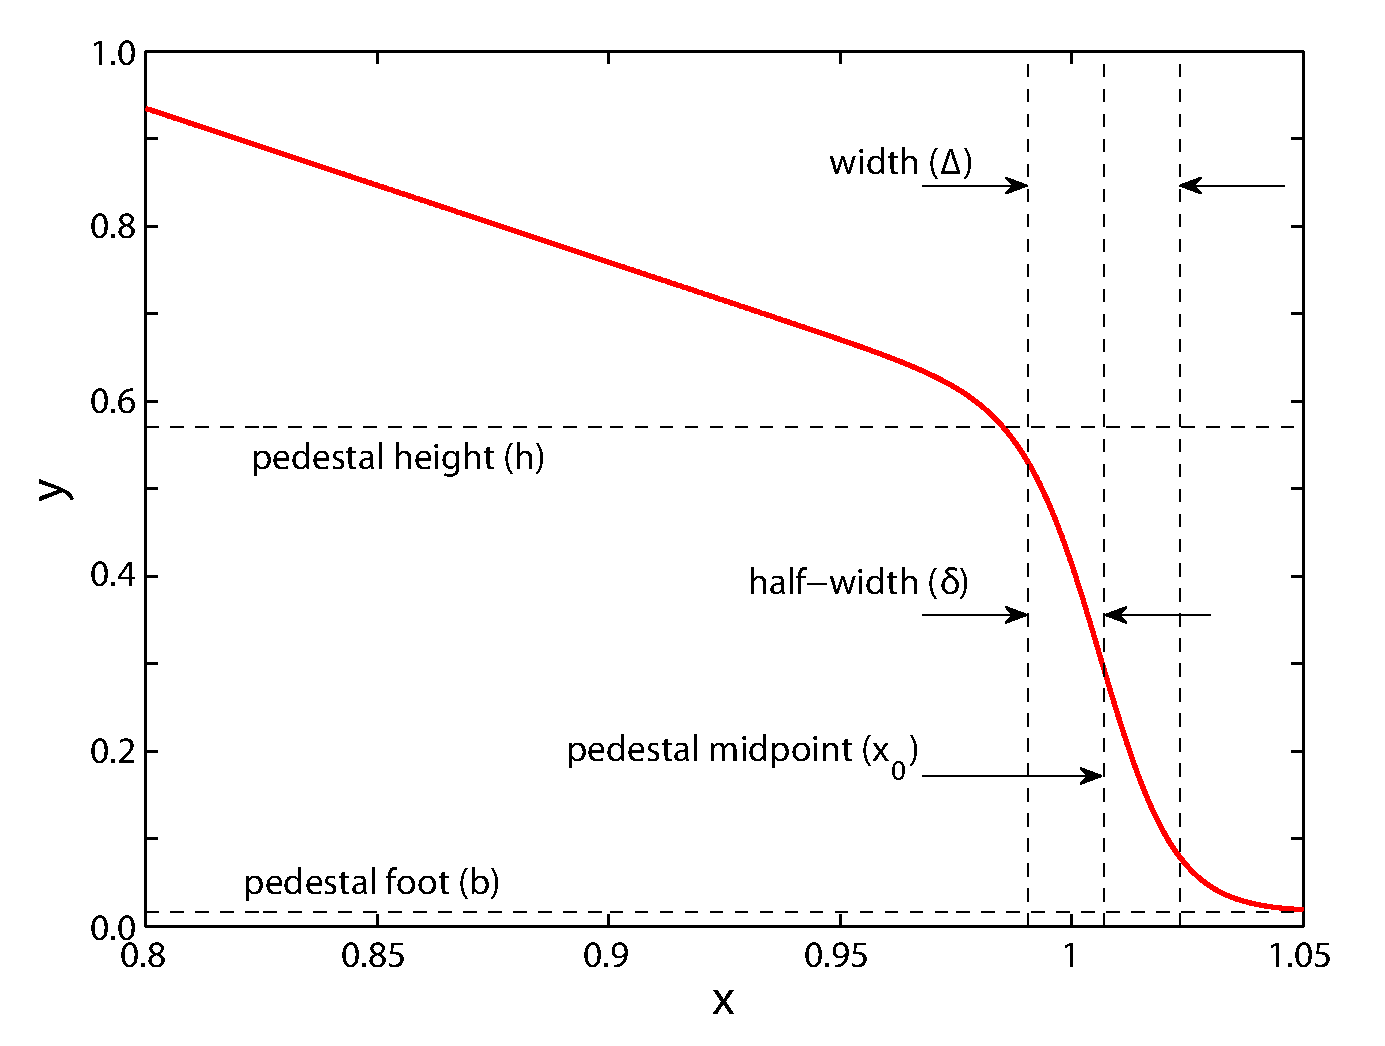
\includegraphics[width=100mm]{graphics/ELMy/mtanh.pdf}}
\end{figure}

The electron density, temperature, and pressure profiles are fitted using a modified hyperbolic-tangent fit developed in \cite{Groebner2001}.  In a general $x,y$ space, the fitting function is expressed by

\begin{equation}\label{eq:mtanh}
 \begin{aligned}
  z &= \frac{x_0 - x}{\delta}\\
  mtanh(\alpha,z) &= \frac{(1 + \alpha z) e^z - e^{-z}}{e^z + e^{-z}}\\
  y &= \frac{h+b}{2} + \frac{h-b}{2} mtanh(\alpha,z)
 \end{aligned}
\end{equation}

\noindent where $x_0$ is the pedestal midpoint, $h$ and $b$ are the height and baseline, and $\delta$ is the half-width (we use $\Delta = 2\delta$ as the ``pedestal width'').  The inboard slope is encoded by the parameter $\alpha$, with the multiplicative factor $1 + \alpha z$ providing a roughly linear profile far from the pedestal.  This definition provides a smooth, continuous definition for the pedestal gradient throughout the profile, with the peak gradient found analytically at $x_0$.\gnote{note similar $n_e$, $T_e$ pedestal widths, EPED width definition}

\nicesectionending

\section{ELM Cycle Synchronization}\label{sec:elmy_sync}

\nicesectionending

\section{EPED Model Predictions}\label{sec:elmy_eped}

\nicesectionending

\section{$I_p$ Scan}\label{sec:elmy_ip}

\nicesectionending

\section{Pedestal Width Scalings}\label{sec:elmy_width}

\nicechapterending

\bibliographystyle{../plainurl}
\bibliography{../references}
\chapter{I-Mode Pedestal Scalings \& Confinement}\label{ch:ImodePedestal}

The I-mode \cite{Whyte2010,Hubbard2011,McDermott2009a,Cziegler2011,Cziegler2013}, introduced in \cref{sec:hcr_imode}, is a novel high-performance regime pioneered on Alcator C-Mod.  I-mode is unique in that it appears to decouple energy and particle transport, forming a steep temperature pedestal with H-mode levels of energy confinement without the accompanying density pedestal or suppression of particle transport found in conventional H-modes (see \cref{fig:imode_trace_ped}).  I-mode exhibits several highly attractive properties for a putative reactor regime:

\begin{enumerate}
 \item Due to the lack of particle transport suppression (as is found in H-modes), the I-mode retains L-mode-like impurity confinement times, avoiding the accumulation of deleterious impurities in the plasma, including those from high-$Z$ metal plasma-facing components necessary for reactor operation \cite{Loarte2007}.  This enables stationary operation without the need for ELMs or continuous fluctuations in the edge to provide the necessary relaxation of the particle confinement.
 \item I-mode appears to be naturally stable against large ELMs, avoiding excessive pulsed heat loading to plasma-facing components without externally-applied engineering controls (described in \cref{subsec:hcr_elmy_control}).
 \item Energy confinement in I-mode appears to exhibit little to no degradation with input heating power, in contrast to that found in ELMy H-mode ($\tau_E \sim P^{-0.7}$ from the ITER98y2 analysis \cite{ITER1999}), scaling quite favorably to reactor-scale devices where fusion self-heating dominates.
\end{enumerate}

%\begin{figure}[t]
% \pushtooutside
% \fcapside[60mm]{\caption[L-mode and I-mode edge profiles from a single discharge.]{L-mode (black) and I-mode (red) edge profiles from a single discharge.  I-mode maintains a comparable density profile (particularly, there is no change in $\nabla n_e$ or formation of a density pedestal), while forming an H-mode-like temperature pedestal.  \note{rescale, add detail?  repeat fig. 2.6?}}\label{fig:imode_pedestal}}{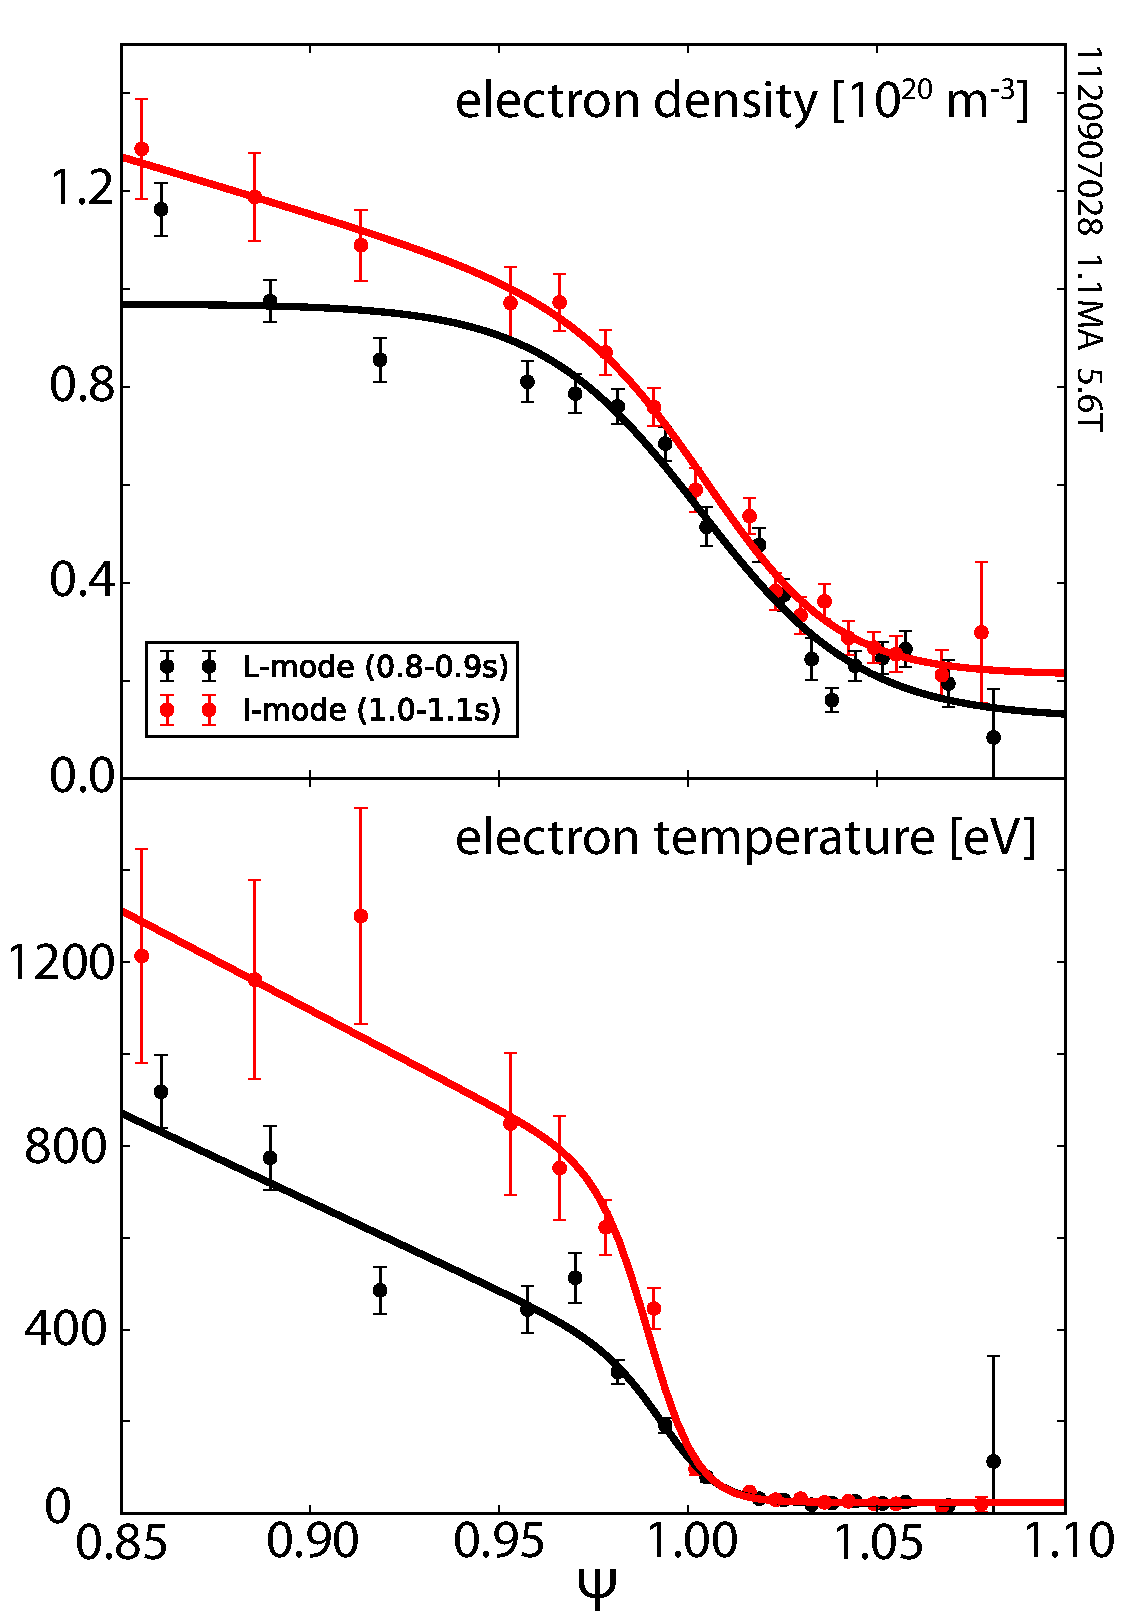
\includegraphics[width=100mm]{graphics/IModePedestal/1120907028_dens_temp.pdf}}
%\end{figure}

\begin{figure}[t]
 \pushtooutside
 \ffigbox[\FBwidth]{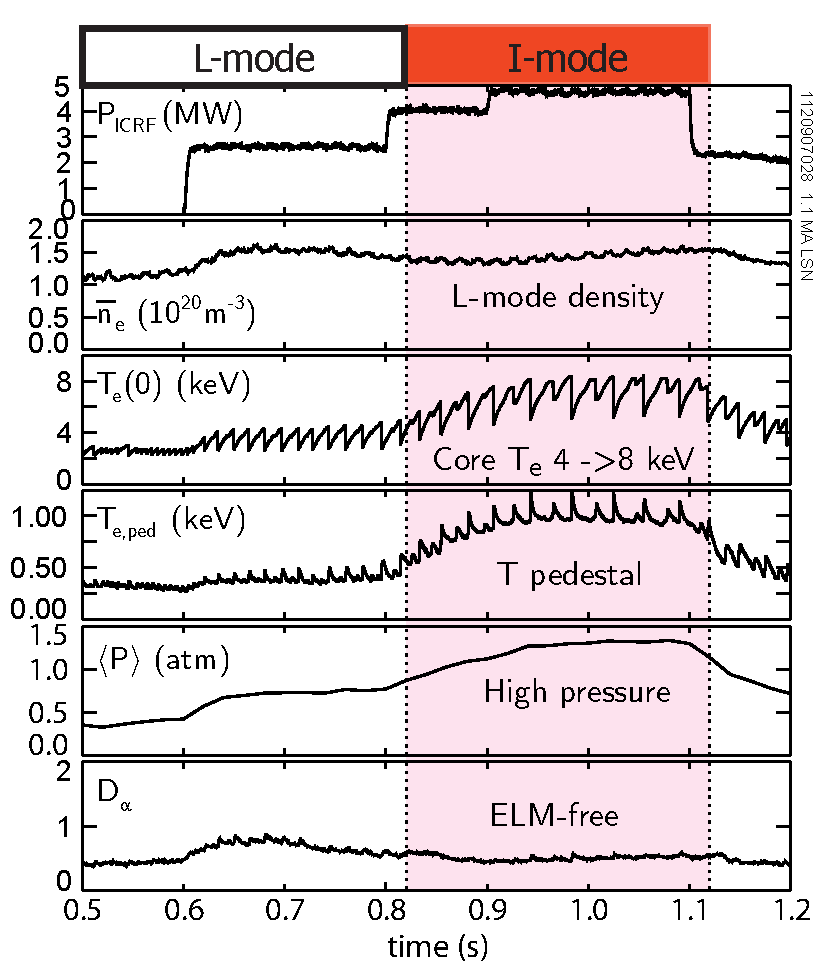
\includegraphics[width=150mm]{graphics/HighPerformanceRegimes/trace_imode.pdf}}{\caption[Characteristic traces for a typical I-mode, and comparisons of I-mode pedestal profiles to L- and H-modes.]{(left) Characteristic traces for a typical I-mode.  At the L-I transition, the core and edge temperature rise over several sawtooth cycles before reaching a steady level; global confinement and pressure rise accordingly.  However, the density remains at L-mode levels, and no ELMs are exhibited.  (right) Edge profiles for density, temperature, and pressure in L-, I-, and H-mode.  The I-mode (green) retains an density profile comparable to the L-mode (black), unlike the ELMy (red) and EDA (blue) H-modes which form a strong density pedestal.  However, the I-mode forms a higher temperature pedestal than either H-mode.  As a result, the I-mode reaches comparable pedestal pressures to the H-modes while retaining L-mode particle transport. (repeated from \cref{fig:hcr_imode_trace})}\label{fig:imode_trace_ped}}
\end{figure}

A firm understanding of the pedestal is essential for the extrapolation of any high-performance regime to ITER- and reactor-scale devices.  The pedestal height sets a strong constraint on core temperature and pressure -- and therefore overall fusion performance -- both by acting as a boundary condition for the plasma profiles, and by supporting steeper core temperature gradients due to profile stiffness \cite{Kinsey2011,Hubbard1998}.  Moreover, the pedestal structure, particularly the steep gradients in density, temperature, and/or pressure, determines stability of the plasma against large, deleterious ELMs (see \cref{sec:mod_pb}).  In this chapter, we present empirical observations of the pedestal in I-mode from a recent series of dedicated experiments \cite{Walk2014}, with a focus on high-resolution pedestal profile measurements across a range of plasma parameters.  Through this, we examine trends in I-mode pedestal behavior, and their impact on global behavior and performance in I-mode, and possible extrapolations to larger devices.\nicesectionending

\section{Access and Experimental Setup}\label{sec:imode_setup}

\begin{figure}[p]
 \pushtooutside
 \fcapside[60mm]{\caption[I-mode edge safety collisionality and safety factor.]{Range in edge collisionality $\nu^*_{95}$ and $q_{95}$ over which I-modes have been accessed.  Notably, I-mode operation is naturally favored near ITER targets for these parameters.  The subset of this data prepared with high-resolution pedestal profiles, herein termed the ``pedestal database'', is also highlighted.}\label{fig:imode_q_nustar}}{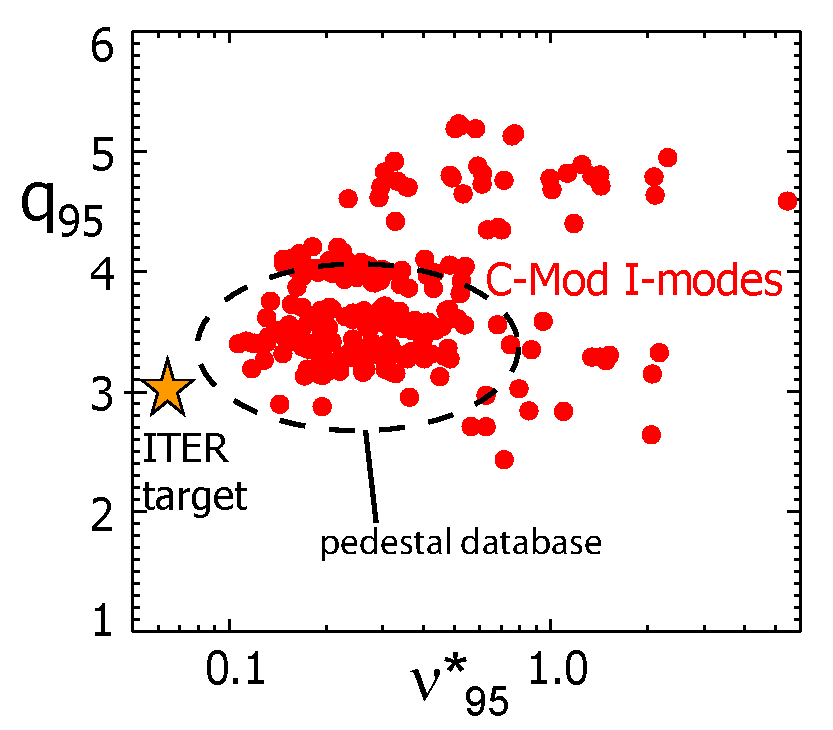
\includegraphics[width=100mm]{graphics/IModePedestal/q95_vs_nustar_2012_Imodeonly.pdf}}
\end{figure}

\begin{figure}[p]
 \pushtooutside
 \fcapside[60mm]{\caption[Density and power range for I-mode access]{Line-averaged density and loss power range for USN and LSN I-modes, illustrating $\sim 2 \times P_{L-I}$ range for I-mode access.  USN shapes are forward-field and LSN-shapes are reversed field, such that all I-modes shown are in the unfavorable drift configuration.  Data from the high-resolution pedestal database (all are LSN reversed-field) are highlighted.}\label{fig:imode_p_nebar_access}}{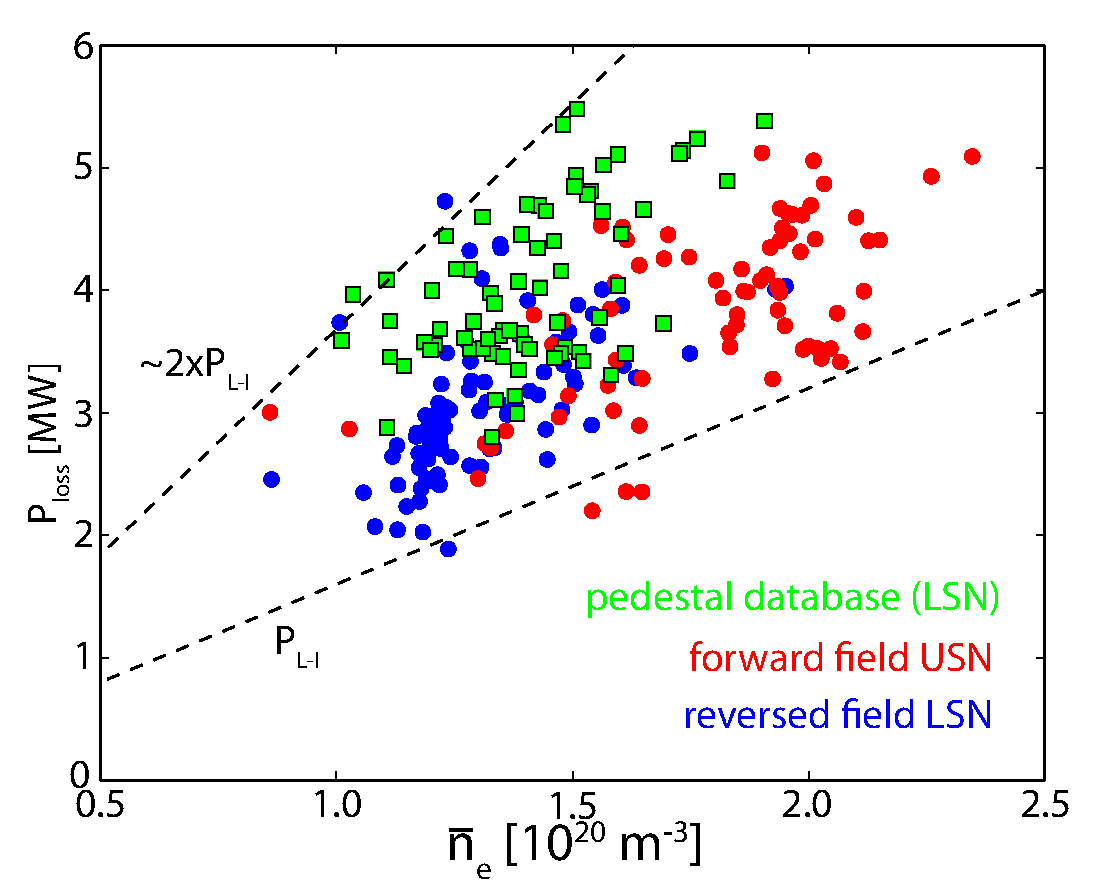
\includegraphics[width=100mm]{graphics/IModePedestal/nebar_Ploss_all.pdf}}
\end{figure}

%\begin{figure}[p]
% \pushtooutside
% \fcapside[60mm]{\caption[Density and power range for I-mode access]{Line-averaged density and loss power range for I-modes in the pedestal database, illustrating $\sim 2 \times P_{L-I}$ range for $1-\SI{1.2}{\mega\ampere}$, $5-\SI{6}{\tesla}$ I-modes.}\label{fig:imode_p_nebar_access}}{\includegraphics[width=100mm]{graphics/IModePedestal/nebar_Pnet.pdf}}
%\end{figure}

All data presented here was taken on the Alcator C-Mod tokamak, described in \cref{sec:intro_cmod}.  As described in \cref{subsec:hcr_imode_access}, I-mode access hinges primarily on operation with the ion $\nabla B$ drift (\cref{eq:gradbdrift}) directed away from the primary X-point in the plasma (the ``unfavorable $\nabla B$ drift'' configuration).  Within this requirement, though, I-mode access is fairly robust, with steady I-modes sustained in a variety of shapes -- both USN with standard field, and LSN shapes with reversed field to achieve the desired $\nabla B$ drift direction (in the latter case, the plasma current is reversed as well to preserve field helicity) -- and edge-current profiles, and at low-to-moderate collisionality (\cref{eq:nustar}).  The attained range in $q_{95}$ and $\nu^*_{95}$ is shown in \cref{fig:imode_q_nustar}.  I-mode has been sustained with heating power up to $\sim 2 \times$ the L-I transition threshold power, which tends to increase approximately linearly with density (see \cref{fig:imode_p_nebar_access}), above which the plasma typically enters an ELM-free H-mode (recall that operating with unfavorable $\nabla B$ drift elevates the H-mode threshold power by roughly a factor of two \cite{Suttrop2003,Carlstrom1998,Groebner1998}).

I-mode experiments in the 2012 run campaign have focused on reversed-field LSN plasmas, which exhibit the widest access window and avoid difficulties with power handling and edge diagnostics.  A subset of results from these experiments have been prepared with high-resolution pedestal measurements, optimized for analysis of the I-mode pedestal structure both from an empirical standpoint and for a computational approach to the pedestal stability; these data, herein termed the ``pedestal database'' (parameter range highlighted in \cref{fig:imode_q_nustar}) is stored in an SQL database (see \cref{app:sql}) for easy access and analysis, and will be used for the bulk of the I-mode work in this thesis (\cref{ch:ImodePedestal,ch:ImodeModeling}).\nicesectionending

\section{Pedestal Responses}\label{sec:imode_height}

To understand the physics of the I-mode pedestal, it is useful to compare the I-mode to established scalings for baseline H-modes.  For the purposes of this discussion, we distinguish between the \emph{MHD-limited} pedestals found in ELMy H-mode (see \cref{sec:hcr_elmy}) and the \emph{transport-limited} pedestals in EDA H-mode (see \cref{subsec:hcr_eda}).  The pedestal structure in the MHD-limited case is determined by peeling-ballooning stability, described in \cref{sec:mod_pb} -- this manifests predominantly as a limit on the pressure gradient due to the instability drive for the ballooning mode, $\alpha_{MHD}$ (see \cref{eq:alphaMHD,eq:alphaMHD_cyl}).  This scales as $\alpha_{MHD} \sim \nabla p / B_p^2$, consistent with the observed $\nabla p \sim I_p^2$ dependence observed in experiments \cite{Walk2012,Groebner2013} (\cf \cref{ch:Elmy}).  To lowest-order approximation, this sets a limit on the pedestal poloidal beta, such that for a given current, field, and shaping configuration the pedestal pressure $p \sim n_e T_e$ is fixed.  Altering the density via fueling results in heating or cooling the pedestal to maintain this limit, while attempts to modify the pedestal via heating power alters the energy transport (increasing the ELM frequency $f_{ELM} \sim P$ for large type-I ELMs \cite{Urano2003}).  In transport-limited EDA H-mode pedestals, on the other hand, the pedestal is controlled in part by the interplay between the strong particle pinch and the continuous outward particle transport driven by the QCM, such that the density tends to lock to a value set by the plasma current.  Within this limit, the pedestal temperature (and therefore pressure) responds positively to increased heating power \cite{Hubbard2001}.

\subsection{Pedestal Temperature}\label{subsec:imode_temp}

As the I-mode is characterized, in part, by its H-mode-like temperature pedestal and energy confinement, that is a suitable place to begin an examination of the I-mode pedestal.  A scan of plasma current from $\num{0.85}$ to $\SI{1.35}{\mega\ampere}$ reveals a positive trend of the pedestal temperature with plasma current, shown in \cref{fig:imode_Ip_Te95} with ELMy H-modes for comparison.  The I-mode temperature pedestal meets or exceeds the pedestal $T_e$ found in H-modes.  This is highly beneficial for global performance, as the high temperature pedestal coupled with stiff core temperature profiles supports very high (up to $\SI{8}{\kilo\electronvolt}$) core temperatures -- with moderately peaked core density profiles, this supports comparable core pressures and fusion reaction rates to H-mode despite the reduced pedestal pressure (see \cref{subsec:imode_pres}).

\begin{figure}
 \pushtooutside
 \fcapside[60mm]{\caption[Pedestal temperature vs. plasma current for I-mode and ELMy H-mode.]{Pedestal temperature versus plasma current for I-mode and ELMy H-mode.  I-mode temperature pedestals meet or exceed H-mode levels, and trend positively with current.  The spread in $T_{e,95}$ at a given current point is due to varying power per particle (see \cref{fig:imode_Pnebar_Te95}).  The highest-current I-modes exhibit temperatures below the bulk trend due to low values of $P_{net}/\overline{n}_e$, as these I-modes were fueled to relatively high densities.}\label{fig:imode_Ip_Te95}}{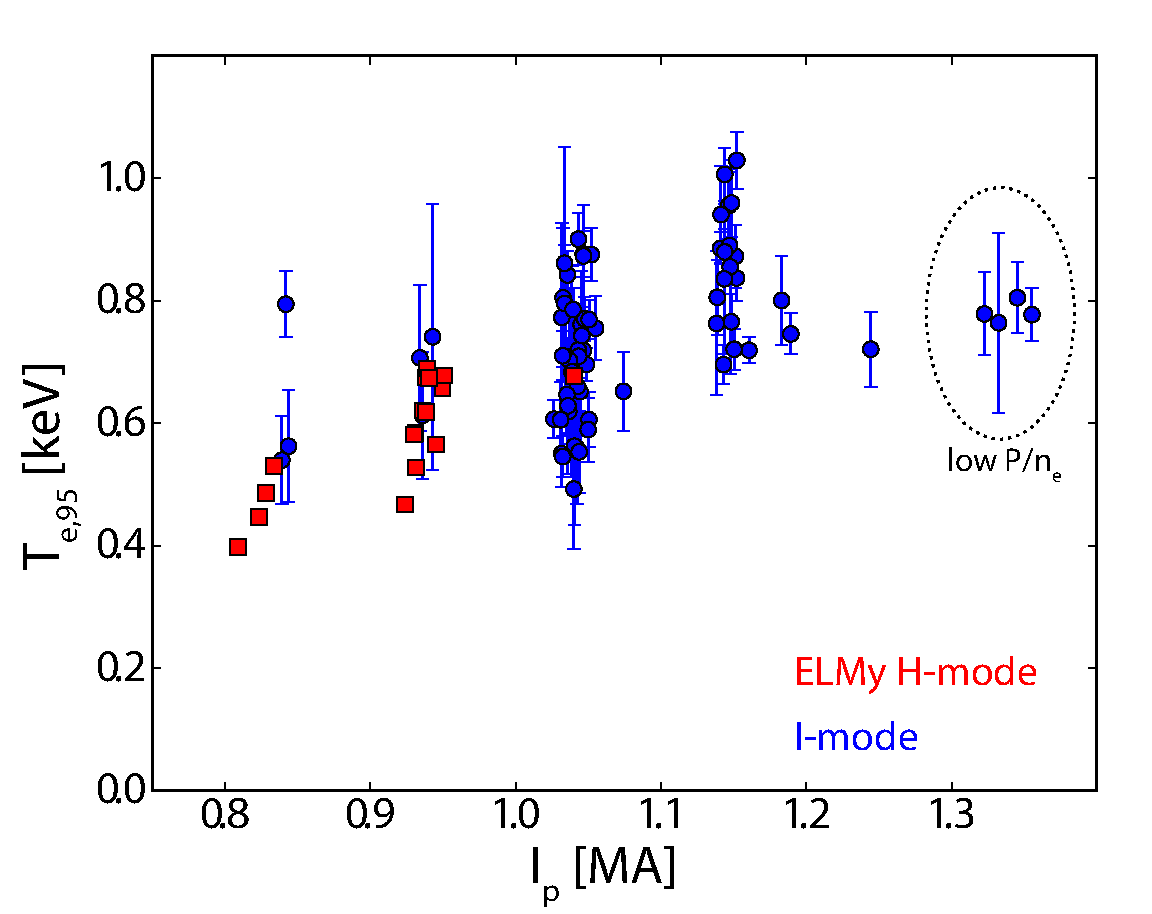
\includegraphics[width=100mm]{graphics/IModePedestal/Ip_Te95.pdf}}
\end{figure}

There is, however, significant scatter at a given point in the $I_p$ scan, due to variation in the input heating power.  Examining a single current slice at $\SI{1.15}{\mega\ampere}$, shown in \cref{fig:imode_Pnebar_Te95}, we see a strong dependence of the temperature pedestal height on the net heating power (\cref{eq:pnet}), normalized to (line-averaged) density -- effectively, the input power per particle.  This same pattern is observed at other current points.  The comparatively suppressed temperatures at the highest-current I-modes is a result of the higher fueling at these points, resulting in lower values of $P_{net}/\overline{n}_e$.  I-modes in these experiments were typically fueled to densities corresponding to Greenwald fractions  (\cref{eq:GDL}) $0.15 \le f_{Gr} \le 0.26$, with the highest-current points at $f_{Gr} \sim 0.2$, or $\SI{1.8e20}{\per\meter\cubed}$.

\begin{figure}
 \pushtooutside
 \fcapside[60mm]{\caption[Pedestal temperature vs. heating power per particle for an example current slice.]{Pedestal temperature $T_{e,95}$ vs. heating power per particle ($P_{net}/\overline{n}_e$) for the $\SI{1.15}{\mega\ampere}$ current slice, illustrating the approximately-linear trend in temperature at fixed current.  This behavior is highly beneficial as an external control for the pedestal temperature.}\label{fig:imode_Pnebar_Te95}}{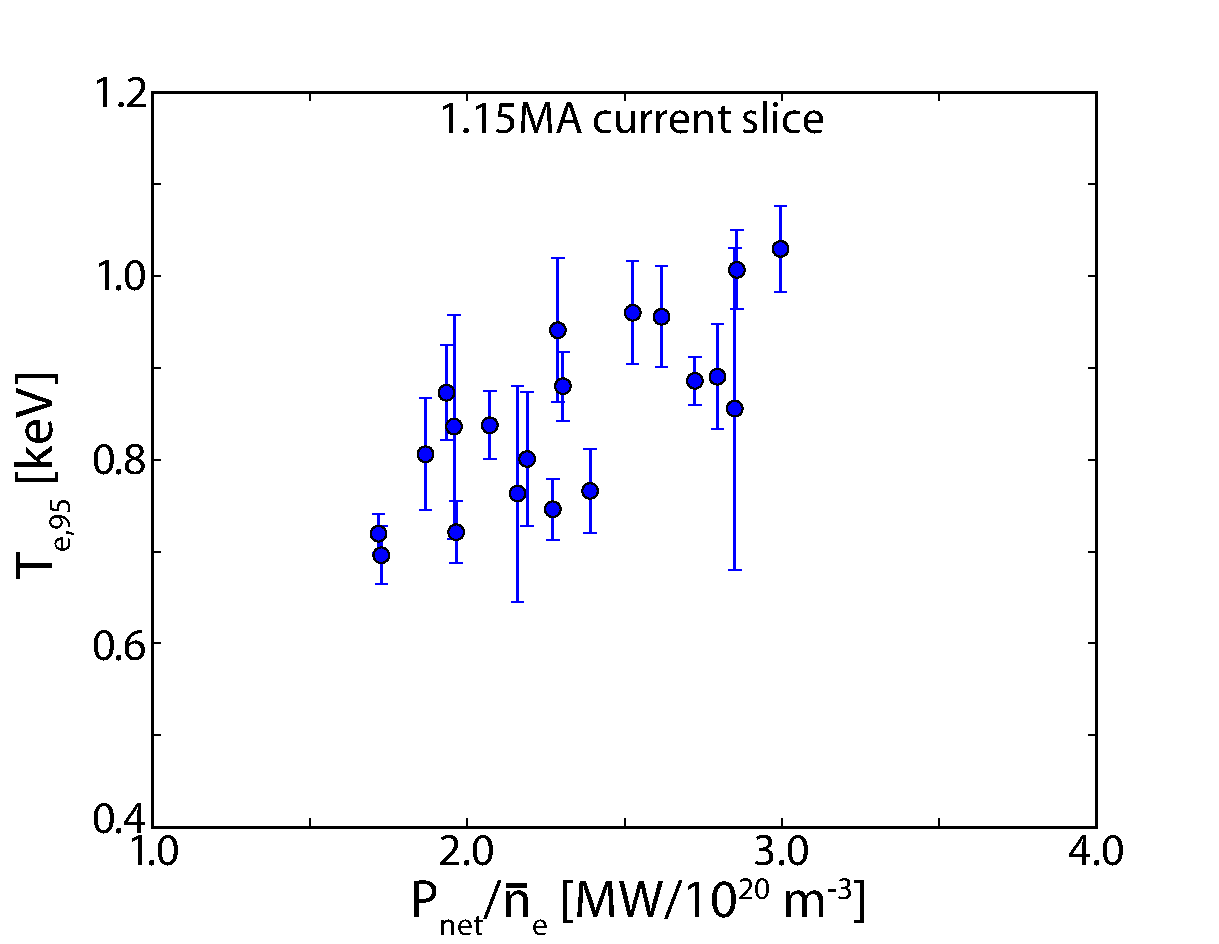
\includegraphics[width=100mm]{graphics/IModePedestal/Pnebar_Te95_115MA.pdf}}
\end{figure}

The temperature pedestal response in I-mode to plasma current is comparable to that seen in the density, temperature, and pressure pedestals in ELMy H-mode (\cf \cref{fig:elmy_ipscan}), although the sensitivity of the temperature pedestal in ELMy H-mode is somewhat weaker than in I-mode.  The response of the temperature pedestal to heating power is notable: the temperature in ELMy H-mode pedestals is only weakly dependent on power -- rather, increased heating power increases the ELM frequency and energy transport to maintain the approximately $\beta_p$-limited pedestal (\cf \cref{fig:hcr_elmybetas,fig:elmy_neBp_TeBp}).  Transport-limited EDA H-mode pedestals exhibit a similar trend, given as $T_{e,ped} \sim \left(P_{net}/\overline{n}_e\right)^{0.5 \pm 0.1}$ in \cite{Hubbard2001} and $T_{e,ped} \sim \left(P_{net}/n_{e,L}\right)^{0.7 \pm 0.1}$ in \cite{Hughes2002}, with the I-mode pedestal responding at least as strongly -- this suggests that I-mode pedestals are not stability-limited. 

\subsection{Pedestal Response to Fueling}\label{subsec:imode_fueling}

In contrast to the temperature pedestal (\cref{subsec:imode_temp}), the edge density in I-mode exhibits markedly different behavior compared to conventional H-modes.  Edge density is set primarily through operator fueling control via gas puffing, maintaining an L-mode-like density profile without the density pedestal found in H-mode.  The pedestal response to fueling is shown at right in \cref{fig:imode_density}.  Compared to transport-limited EDA pedestals, the plasma current is insufficient as a predictor of I-mode pedestal density, with the positive trend (shown at left in \cref{fig:imode_density}) due to the strong co-variance between $I_p$ and $\overline{n}_e$.

\begin{figure}[ht]
 \pushtooutside
 \ffigbox[\FBwidth]{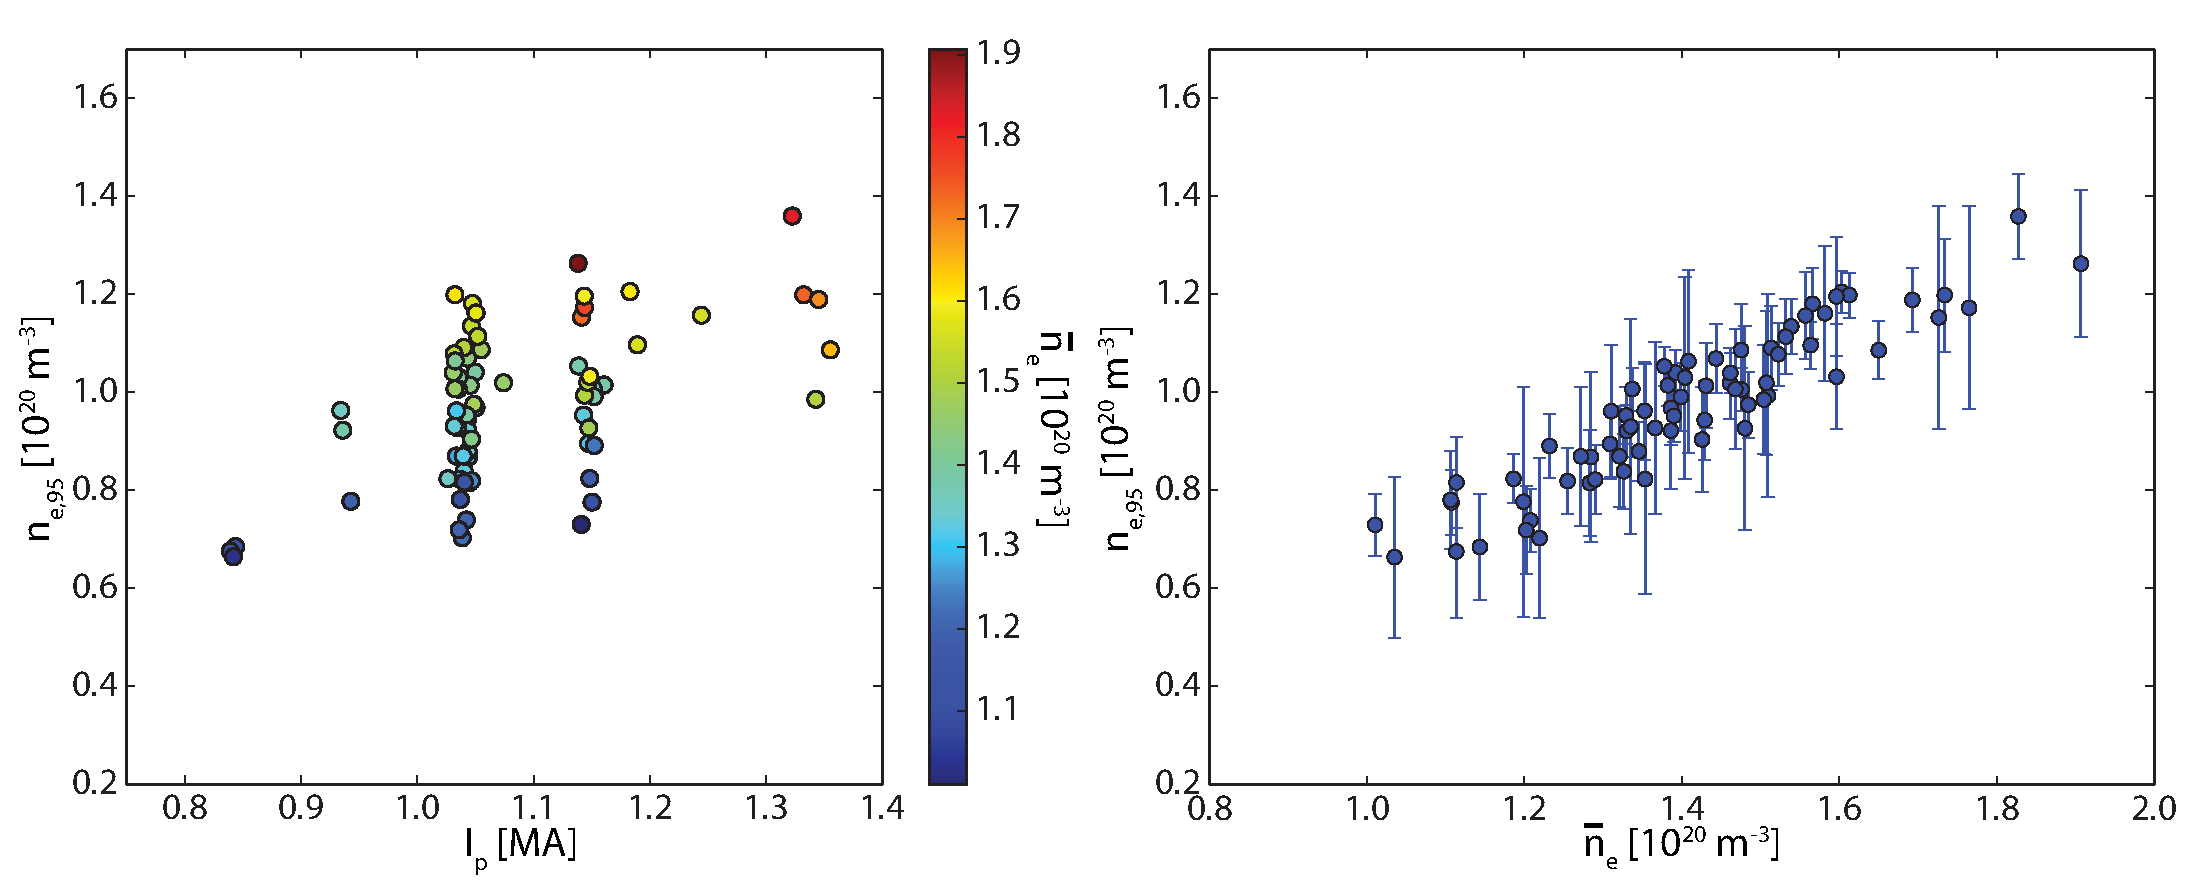
\includegraphics[width=150mm]{graphics/IModePedestal/imode_density.pdf}}{\caption[Pedestal density response to current and fueling.]{Pedestal density as a function of current (left, colored by $\overline{n}_e$) and line-averaged density (right).  The pedestal density is set solely by operator fueling; in contrast the transport-limited pedestals in EDA H-mode, plasma current is a poor predictor of the pedestal density, with the trend due only to the co-variance between $I_p$ and $\overline{n}_e$.}\label{fig:imode_density}}
\end{figure}

\begin{figure}[ht]
 \pushtooutside
 \fcapside[60mm]{\caption[Density and temperature pedestals at matched current and field with varying fueling and heating power -- matched $P_{net}/\overline{n}_e$ maintains the $T_e$ pedestal.]{Density and temperature pedestals at matched current, field, and shaping, with varying fueling and heating power levels.  The three discharges are fueled to $\overline{n}_e$ of $\num{1.0}$ (black), $\num{1.3}$ (blue), and $\SI{1.7e20}{\per\meter\cubed}$ (red) respectively, with heating powers of $\num{2.75}$, $\num{3.65}$, and $\SI{4.10}{\mega\watt}$ to maintain matched $P_{net}/\overline{n}_e \sim 2.4-2.7$.  The constant power-per-particle maintains matched temperature pedestals across the fueling range, indicative of the independent control of pedestal $n_e$ and $T_e$ available in I-mode.}\label{fig:imode_fuelingprofiles}}{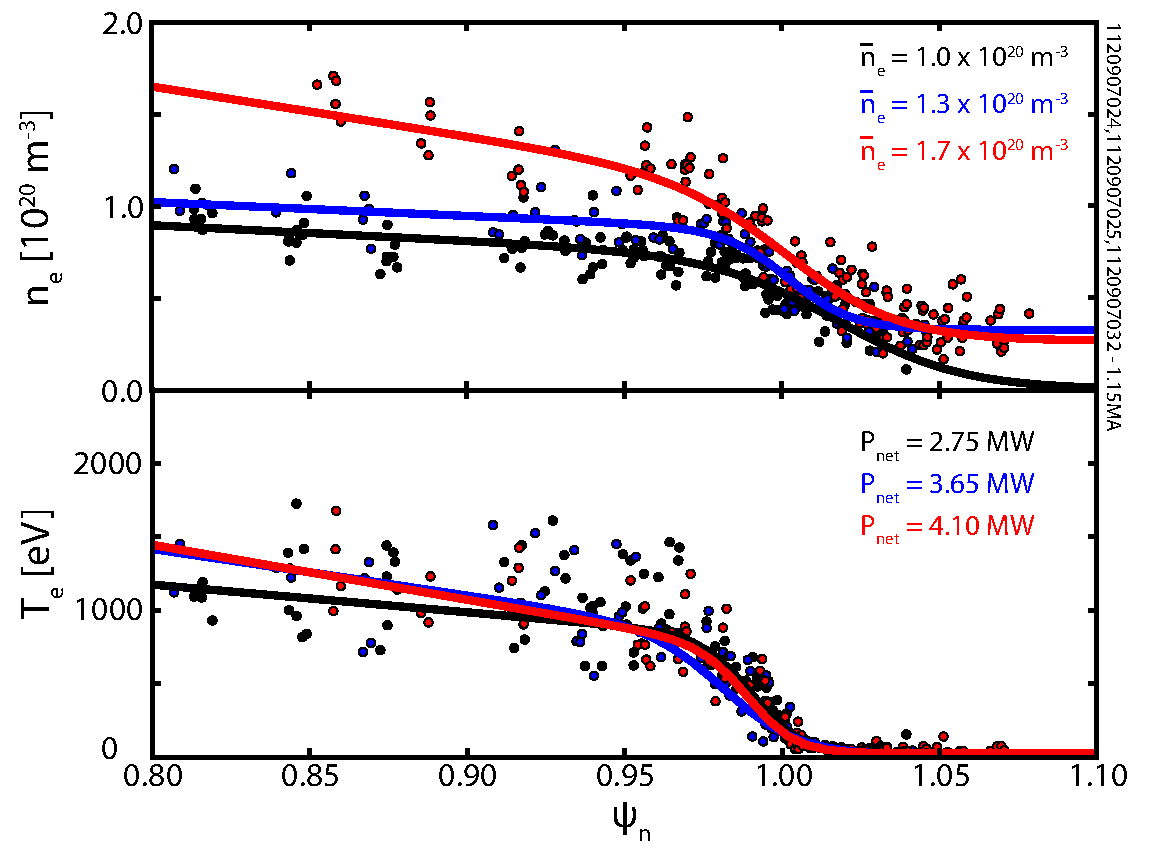
\includegraphics[width=100mm]{graphics/IModePedestal/fuelingprofiles.pdf}}
\end{figure}

Given sufficient heating power, temperature pedestals can be maintained with increased density due to the strong response of $T_{e,95}$ to power-per-particle.  Example discharges matched in current, field, and shaping are shown in \cref{fig:imode_fuelingprofiles}, spanning a range in fueling and heating power, $\overline{n}_e = 1.0 - \SI{1.7e20}{\per\meter\cubed}$, $P_{net} = 2.75 - \SI{4.10}{\mega\watt}$.  Temperature pedestals are matched across all three discharges, using consistent power-per-particle $P_{net}/\overline{n}_e = 2.4 - \SI{2.7}{\mega\watt}/10^{20}\;\si{\per\meter\cubed}$.

This behavior is distinct from that found in H-modes on C-Mod.  ELMy H-modes at fixed current and shaping exhibit an inverse relationship between pedestal $n_e$ and $T_e$ due to limited pedestal $\beta_p$, such that increased fueling tends to cool the pedestal (although the modification of pedestal collisionality also modifies the ELM character).  EDA H-modes lack the fueling control found in I-mode, instead railing the pedestal density to a value set by the plasma current, such that the outward transport and strong inward particle pinch are balanced.  The largely-decoupled behavior of the density and temperature profiles in the edge in I-mode are highly desirable from an operational standpoint -- fueling (done entirely via edge gas puffing on C-Mod) and heating power are separated as ``knobs'' for plasma and pedestal control, granting significant operational freedom compared to the relatively-constrained H-mode pedestal behavior.

The phenomenon demonstrated in \cref{fig:imode_fuelingprofiles} is indicative of a path to strongly improved performance in I-mode, increasing pedestal $\beta_p$ and global confinement via matched increases in fueling and heating power, maintaining the target temperature pedestal with appropriate levels of $P_{net}/\overline{n}_e$.  Recent experiments on C-Mod \cite{Hubbard2012} have successfully applied this approach, reaching elevated density by fueling into an established I-mode in combination with increased heating power levels, reaching heating power levels that would trigger a transition to H-mode in a comparable-density L-mode.  This L-mode-like density profile is also of great benefit for operation on ITER-scale devices -- due to the high edge density (both observed on C-Mod, and expected for ITER) neutral penetration into the pedestal is expected to be very low.  The strong inward turbulent particle pinch \cite{Kesner2012} in L-mode (and equivalently, I-mode) density profiles is highly desirable for core fueling, as neutral puffing alone is unlikely to be sufficient for core fueling on ITER.

\begin{figure}[h]
 \pushtooutside
 \fcapside[60mm]{\caption[Pedestal pressure versus plasma current in I-mode and ELMy H-mode.]{Pedestal thermal pressure ($2 \times p_{e,95}$) versus plasma current, colored by fueling level indicated by line-averaged density $\overline{n}_e$.  The shaded region indicates the typical range of pedestal pressures in C-Mod ELMy H-modes.  A strong, roughly $p_{95} \sim I_p$ trend in pedestal pressure is observed.  At a given current, a strong increase in pedestal pressure with fueling is also observed (note: heating power also varied in these discharges).}\label{fig:imode_Ip_p95}}{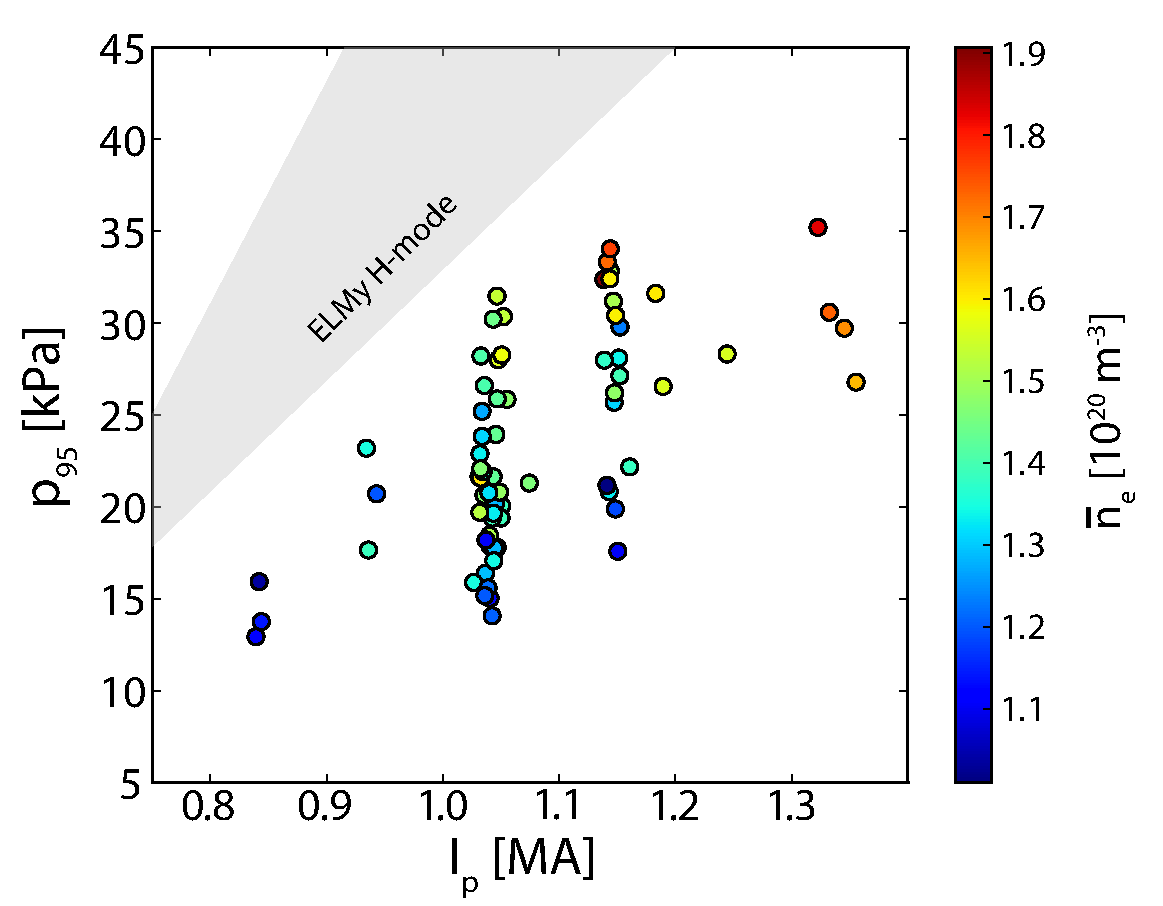
\includegraphics[width=100mm]{graphics/IModePedestal/Ip_p95_nebar.pdf}}
\end{figure}

\subsection{Pressure Pedestal Scalings and Performance}\label{subsec:imode_pres}

Despite lacking a density pedestal, I-mode is capable of reaching pedestal thermal pressures comparable to H-mode, while maintaining favorable behavior  in its particle (particularly impurities -- see \cref{fig:hcr_imode_taui}) transport and temperature pedestal.  I-mode pedestal pressure (we use twice the electron pressure from Thomson Scattering here, consistent with $T_i \approx T_e$ measurements in well-equilibrated pedestals on C-Mod \cite{Hubbard2011} and with the relatively low impurity contribution to the pressure, $Z_{eff} \sim 2$) versus plasma current is shown in \cref{fig:imode_Ip_p95}, with additional differentiation by fueling level indicated by color.  An increase in pedestal pressure by at least $p_{95} \sim I_p$ is observed, consistent with the scaling of the temperature pedestal $T_e \sim I_p$.  The pedestal pressure at a given current is seen to increase strongly with increased fueling, consistent with the maintenance of the temperature pedestal with increased heating power and matched fueling, thus constant levels of $P_{net}/\overline{n}_e$.  I-mode pedestal pressure is reduced from that typically found in H-mode (the typical range in ELMy H-mode is indicated by the shaded region in \cref{fig:imode_Ip_p95}).  This is due to the reduced pedestal density in I-mode compared to H-mode, as the temperature pedestals found in I-mode typically meet or exceed H-mode levels.  The pressure pedestal is expected to be ultimately limited by the ELM trigger -- however, the independent density and temperature pedestal control should allow I-mode to approach, but not exceed, the ELMing limit.

\begin{figure}[t]
 \pushtooutside
 \fcapside[60mm]{\caption[Pedestal pressure vs. heating power for an example current slice.]{Pedestal pressure ($2\times p_{e,95}$) versus net heating power for the $\SI{1.15}{\mega\ampere}$ current slice, illustrating the trend $p_{95} \sim P_{net}$ at fixed current.  This is consistent with the power trend in the I-mode temperature pedestal, $T_{e,95} \sim P_{net}/\overline{n}_e$.}\label{fig:imode_Pnet_p95}}{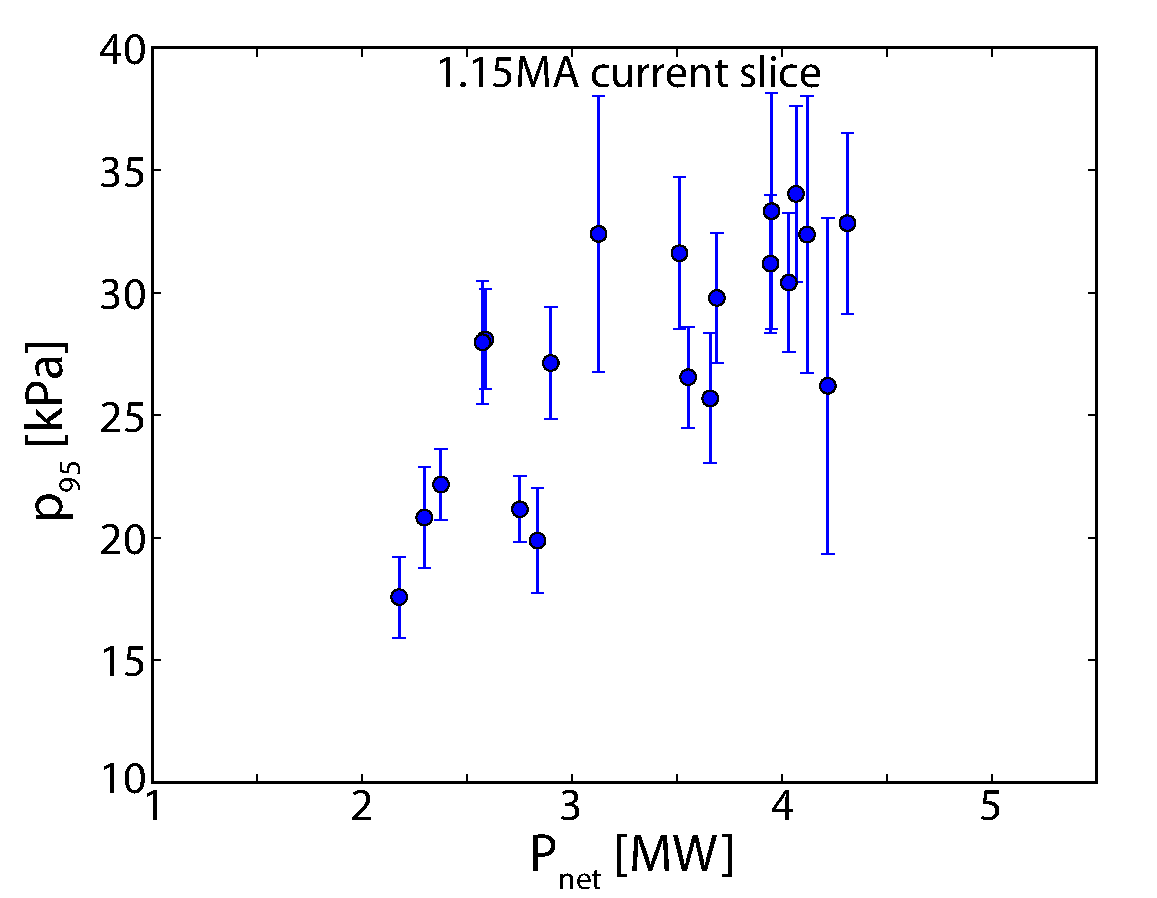
\includegraphics[width=100mm]{graphics/IModePedestal/Pnet_p95_115MA.pdf}}
\end{figure}

\begin{figure}[t]
 \pushtooutside
 \fcapside[60mm]{\caption[Stored energy versus pedestal pressure.]{I-mode stored energy versus pedestal pressure, confirming the strong dependence of global performance on the pedestal height.}\label{fig:imode_p95_W}}{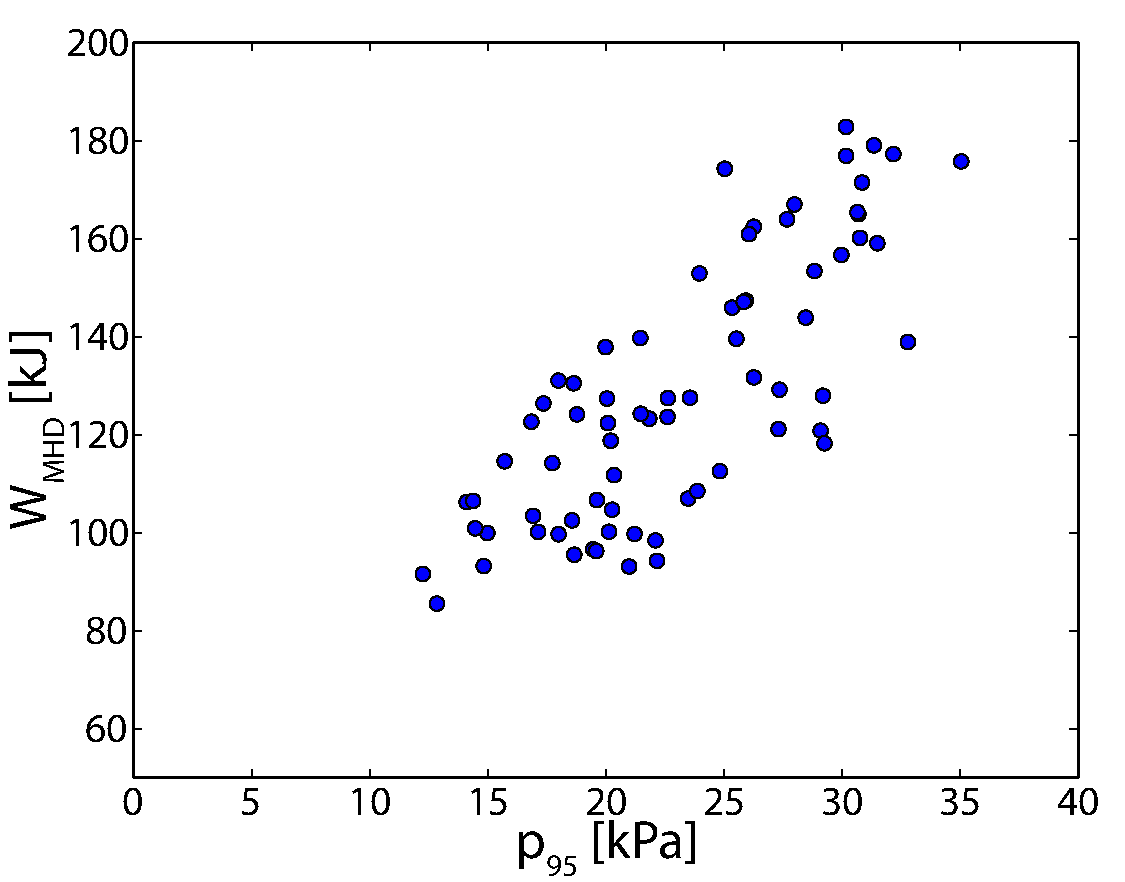
\includegraphics[width=100mm]{graphics/IModePedestal/p95_W.pdf}}
\end{figure}

\begin{figure}
 \pushtooutside
 \fcapside[60mm]{\caption[Pressure gradient vs. plasma current for I-mode and ELMy H-mode.]{Peak pressure gradient (measured at the pedestal midpoint) versus plasma current for I-mode and ELMy H-mode.  I-mode consistently exhibits a weaker pressure gradient at a given current, as well as scaling more weakly than the $\nabla p \sim I_p^2$ expected from the ballooning MHD stability limits associated with ELMy H-mode.}\label{fig:imode_ip_gradp}}{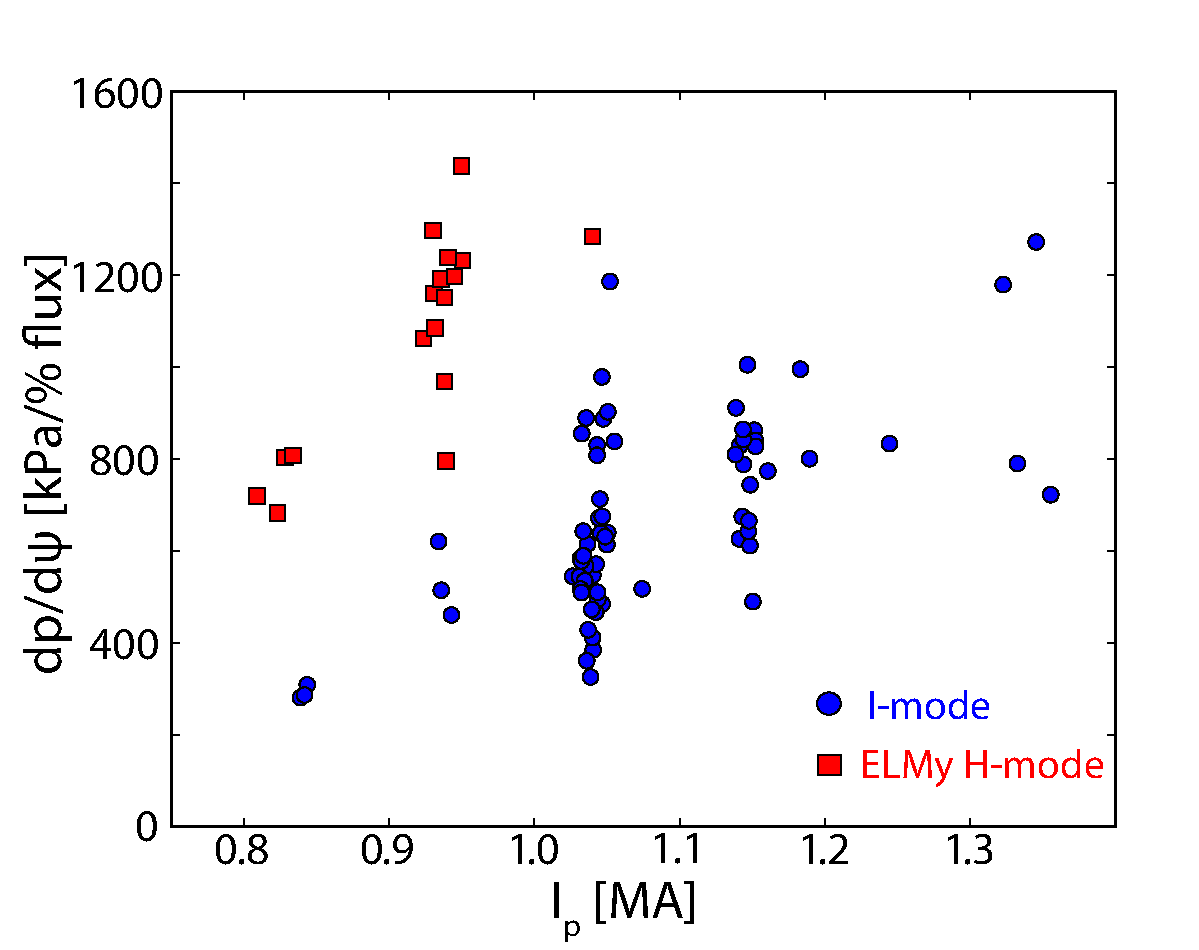
\includegraphics[width=100mm]{graphics/IModePedestal/Ip_gradp.pdf}}
\end{figure}

The effect of heating power on the pressure pedestal is visible in \cref{fig:imode_Pnet_p95}, showing the $\SI{1.15}{\mega\ampere}$ current slice (see \cref{fig:imode_Pnebar_Te95} for the same).  At fixed current, the pressure pedestal scales as $p_{95} \sim P_{net}$, consistent with the previously observed $T_{e,95} \sim P_{net}/\overline{n}_e$ trend in the temperature pedestal as $p_{95} \sim n_{e,95} T_{e,95}$.  This corresponds the favorable scaling of energy confinement in I-mode with heating power -- plasma stored energy is set by heating power and the energy confinement time, $W \sim P \tau_E$, and is strongly influenced by the pedestal pressure (see \cref{fig:imode_p95_W}).  Thus, the trend $p_{95} \sim P_{net}$ is consistent with little or no degradation of $\tau_E$ with heating power, which has been observed in global measurements of I-mode \cite{Dominguez2012,Whyte2010}, and is distinct from the trend $\tau_E \sim P^{-0.7}$ found for ELMy H-modes \cite{ITER1999}.  This behavior is quite favorable when scaled to large, high-power machines, particularly in scenarios with a significant degree of fusion self-heating, where the plasma pressure directly determines heating power via the fusion reaction rate ($\sim p^2$).

Trends in the pressure pedestal in I-mode are also informative to its MHD stability.  As shown in \cref{fig:imode_ip_gradp}, the peak pressure gradient (identified as the driver for ballooning MHD instabilities, described in \cref{subsec:mod_balloon}, and the trigger for large ELMs) in I-mode is consistently shallower at a given $I_p$ than comparable ELMy H-modes on C-Mod, due to the flat edge density profile.  Moreover, the pedestal pressure gradient scales more weakly than the expected $\nabla p \sim I_p^2$ expected from the ballooning stability boundary \cite{Connor1978}.  The intuitive conclusion from this is that I-mode is generally stable to the MHD instabilities identified with the ELM trigger -- the MHD stability and ELM behavior of I-mode is explored in detail in \cref{ch:ImodeModeling}.\nicesectionending

\section{Pedestal Widths}\label{sec:imode_width}

Conventionally, H-mode pedestals are found to be constrained by critical-gradient-driven instabilities, such that the peak $\nabla p$ is limited -- therefore, the width of the transport barrier sets a constraint on the attainable pedestal height (and thus global performance).  Due to the small spatial scales inherent in the pedestal, accurate measurement of the pedestal width has historically been quite difficult, although a number of theoretical models have been proposed and tested against experimental observations, \eg \cite{Maggi2010,Beurskens2011,Onjun2002}.  This section explores a range of potential explanations for the observed pedestal widths in I-mode.

\subsection{Kinetic-Ballooning Limited Pedestals}\label{subsec:imode_kbm}

%The edge turbulence in I-mode is characterized by a strong reduction in mid-frequency turbulence and the appearance of a higher-frequency ($\sim 200 - \SI{400}{\kilo\hertz}$) fluctuation, dubbed the \emph{Weakly-Coherent Mode} or WCM \cite{Whyte2010,Hubbard2011,Dominguez2012,Cziegler2011,Cziegler2013,White2011}.\gnote{not sure I like this intro}  The WCM appears to be connected to the density pumpout and pedestal regulation in I-mode, with the WCM amplitude shown to be correlated to the particle flux through the LCFS \cite{Dominguez2012}.  An understanding of the turbulent behavior in the I-mode pedestal, then, is essential to the extrapolation of I-mode operation to larger devices.  Kinetic-ballooning mode (KBM) turbulence, described in \cref{sec:mod_turbulence}, is thought to constrain the pedestal in ELMy H-mode, and is therefore an important starting point for investigating the WCM.

\begin{figure}[t]
 \pushtooutside
 \fcapside[60mm]{\caption[Pedestal width vs. poloidal beta in I-mode and ELMy H-mode.]{Pedestal width versus poloidal beta in I-mode and ELMy H-mode.  ELMy H-modes lie on the $\Delta_\psi \sim \beta_{p,ped}^{1/2}$ line predicted for KBM-limited pedestals (see \cref{subsec:elmy_eped_width}).  I-mode shows no scaling of the pedestal width with $\beta_p$, and exhibits pedestals consistently wider than predicted for comparable ELM-limited pedestals.}\label{fig:imode_wid_betapol}}{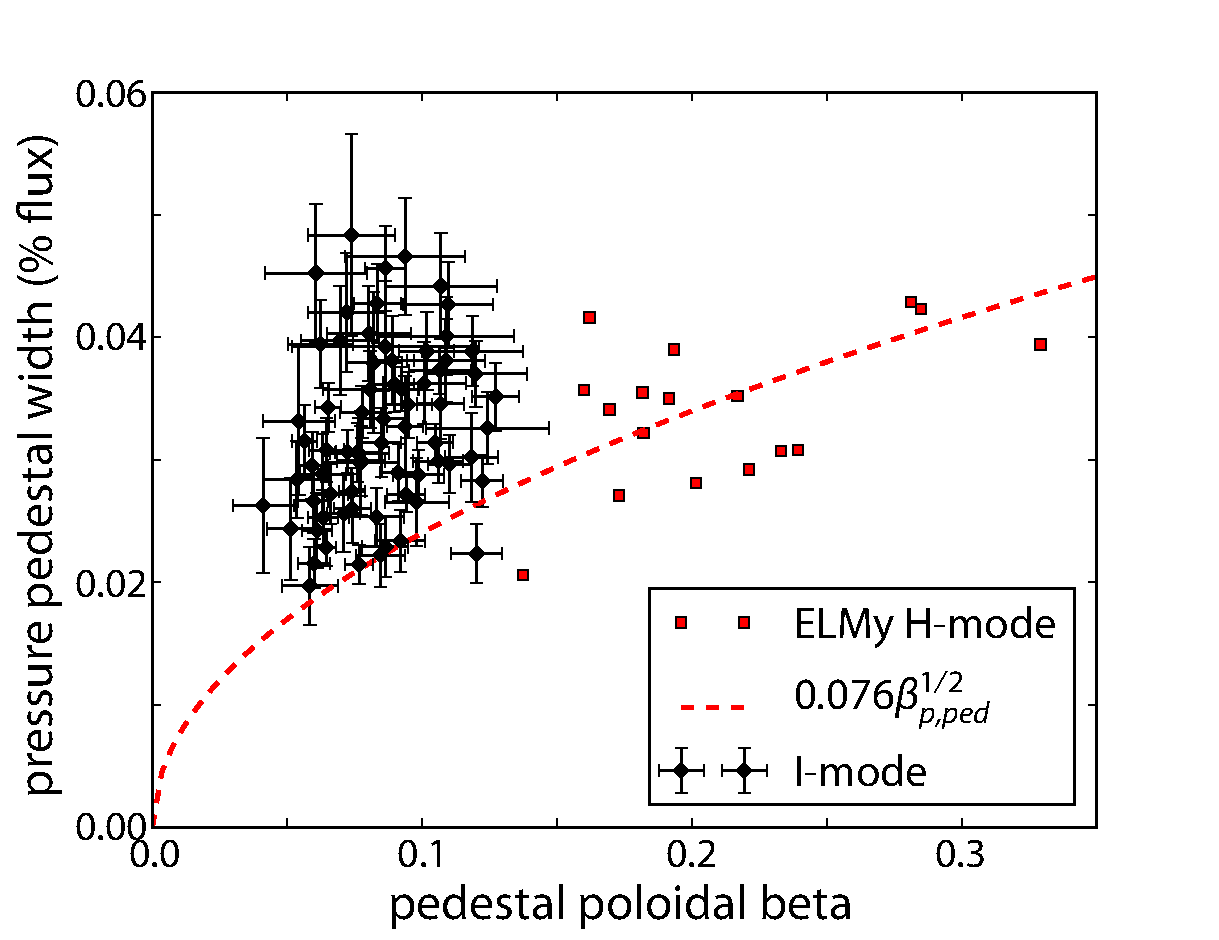
\includegraphics[width=100mm]{graphics/IModePedestal/wid_betapol.pdf}}
\end{figure}

The kinetic-ballooning mode (KBM), described in \cref{sec:mod_turbulence}, applies a constraint to the pedestal width of the form $\Delta \sim \beta_{p,ped}^{1/2}$, where $\Delta$ is the pedestal width in normalized poloidal flux.  This trend has been observed on several machines \cite{Groebner2013,Beurskens2011,Osborne1998}, including on C-Mod (see \cref{ch:Elmy}).  This constraint is used in the EPED model series, described in \cref{sec:mod_eped}.  The simplest implementation of the constraint, used in EPED1 (\cref{subsec:mod_eped1}) uses a fitted coefficient, $\Delta = 0.076 \beta_{p,ped}^{1/2}$ \cite{Snyder2009}.  A comparison of I-mode pedestals against this predictive line, as well as example ELMy H-modes, is shown in \cref{fig:imode_wid_betapol}.  I-mode pedestals are wider on average than predicted by the KBM-limited ($\sim \beta_{p,ped}^{1/2}$) line, and show no trend of pedestal width with poloidal beta.  This suggests that the I-mode pedestal is not constrained by KBM turbulence, consistent with the relaxed pressure gradient found in I-mode -- stability against the KBM is examined in more detail in \cref{sec:imode_baloo}.

\subsection{Local Physics Parameters}\label{subsec:imode_exp_widths}

\begin{figure}[p]
 \pushtooutside
 \ffigbox[\FBwidth]{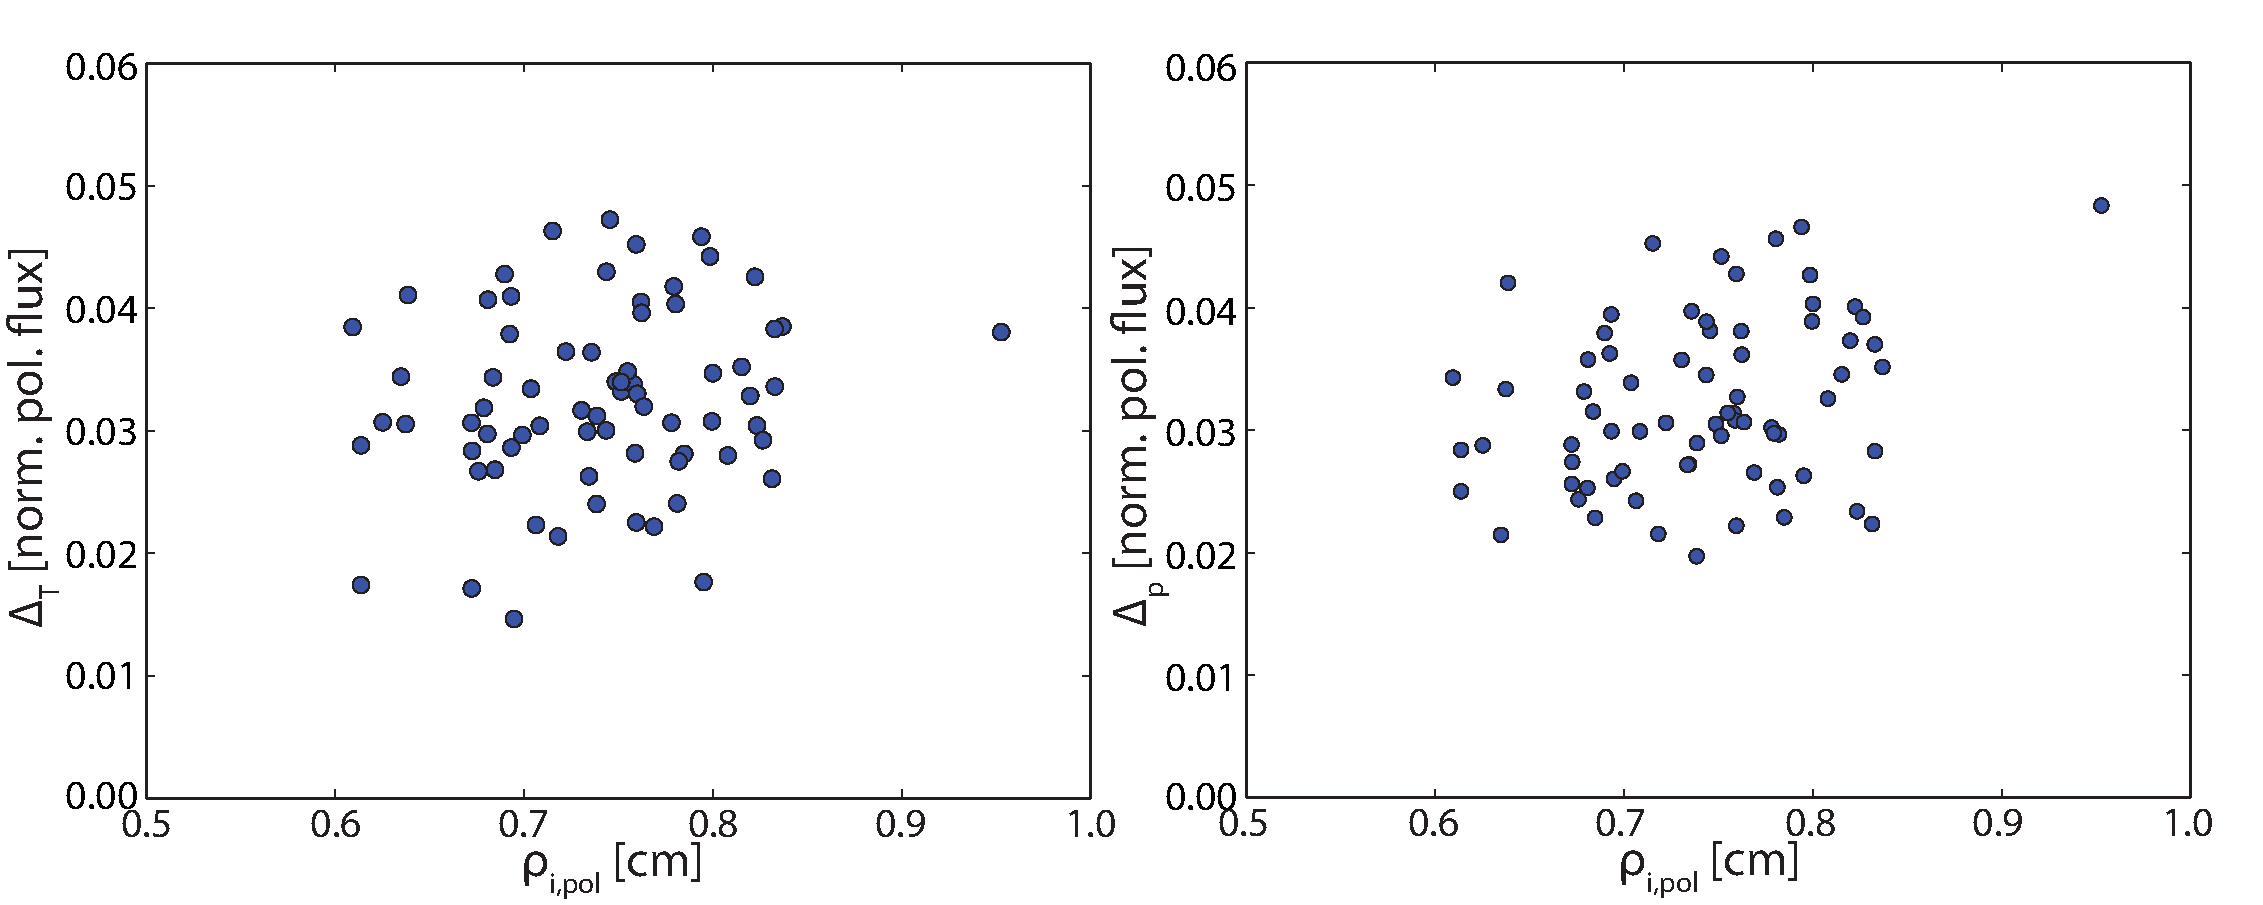
\includegraphics[width=150mm]{graphics/IModePedestal/rhoipol_widths.pdf}}{\caption[Temperature and pressure pedestal width vs. poloidal gyroradius.]{Temperature (left) and pressure (right) pedestal widths versus poloidal gyroradius $\rho_{i,pol}$.  No correlation in the pedestal width is seen, contrary to models suggesting a scaling of the sheared-flow layer and pedestal with the gyroradius.}\label{fig:imode_rhoipol_wid}}
\end{figure}

\begin{figure}[p]
 \pushtooutside
 \ffigbox[\FBwidth]{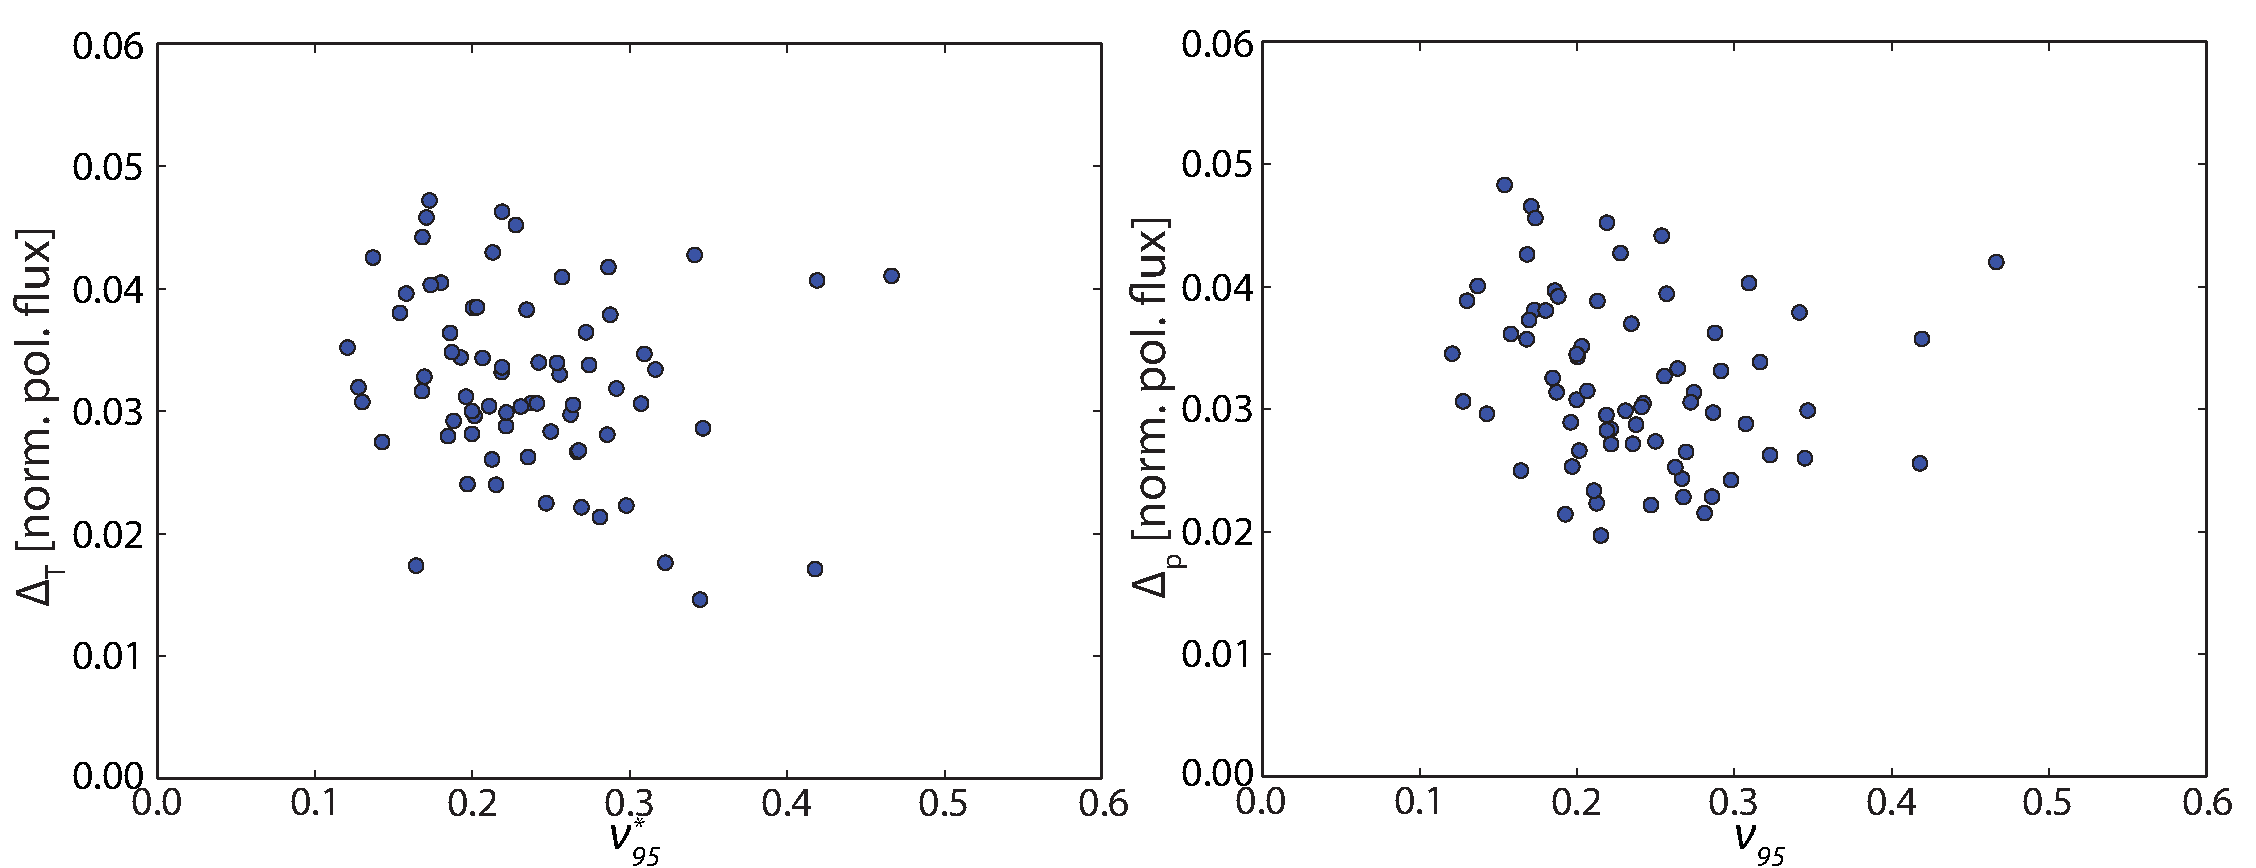
\includegraphics[width=150mm]{graphics/IModePedestal/nustar_widths.pdf}}{\caption[Temperature and pressure pedestal widths vs. pedestal collisionality.]{Temperature (left) and pressure (right) pedestal widths versus pedestal collisionality $\nu^*_{95}$.  No correlation is seen.}\label{fig:imode_nustar_wid}}
\end{figure}

\begin{figure}[p]
 \pushtooutside
 \ffigbox[\FBwidth]{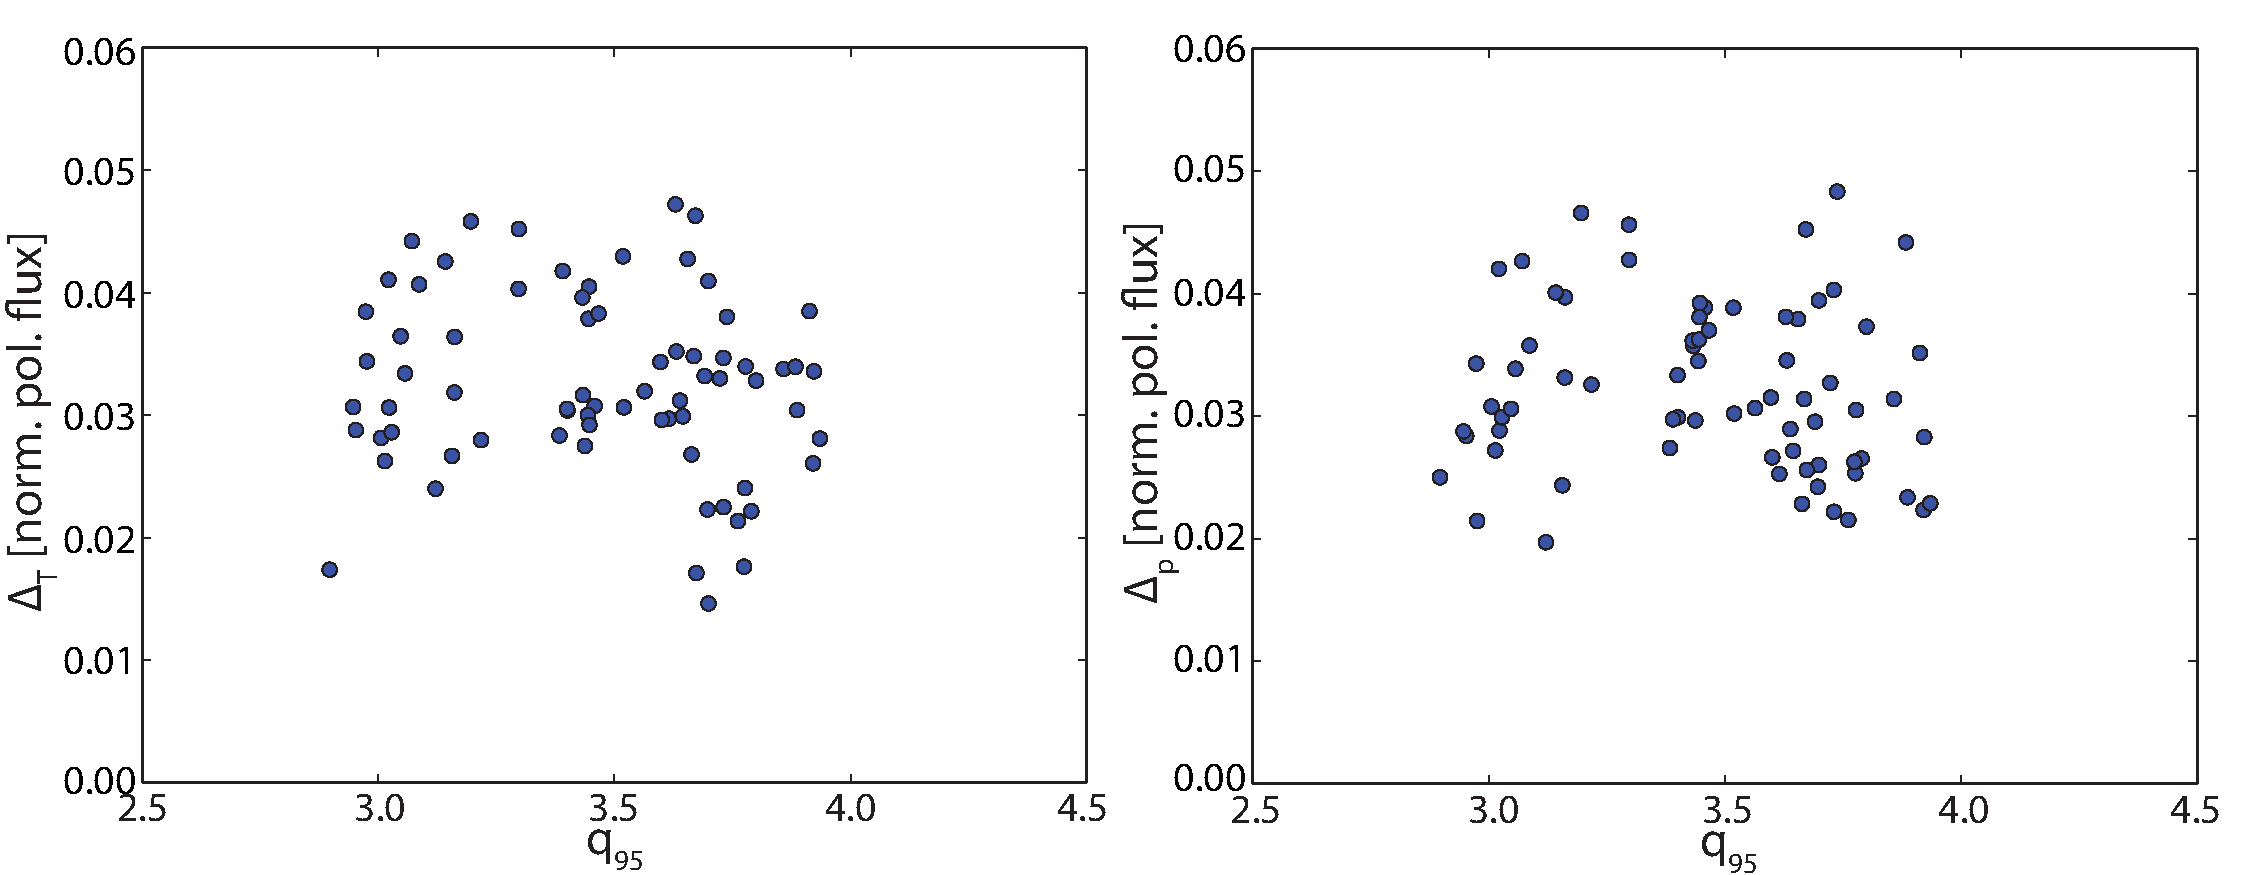
\includegraphics[width=150mm]{graphics/IModePedestal/q95_widths.pdf}}{\caption[Temperature and pressure pedestal widths vs. edge safety factor.]{Temperature (left) and pressure (right) pedestal widths versus edge safety factor $q_{95}$.  No correlation is seen.}\label{fig:imode_q95_wid}}
\end{figure}

\begin{figure}[t]
 \pushtooutside
 \ffigbox[\FBwidth]{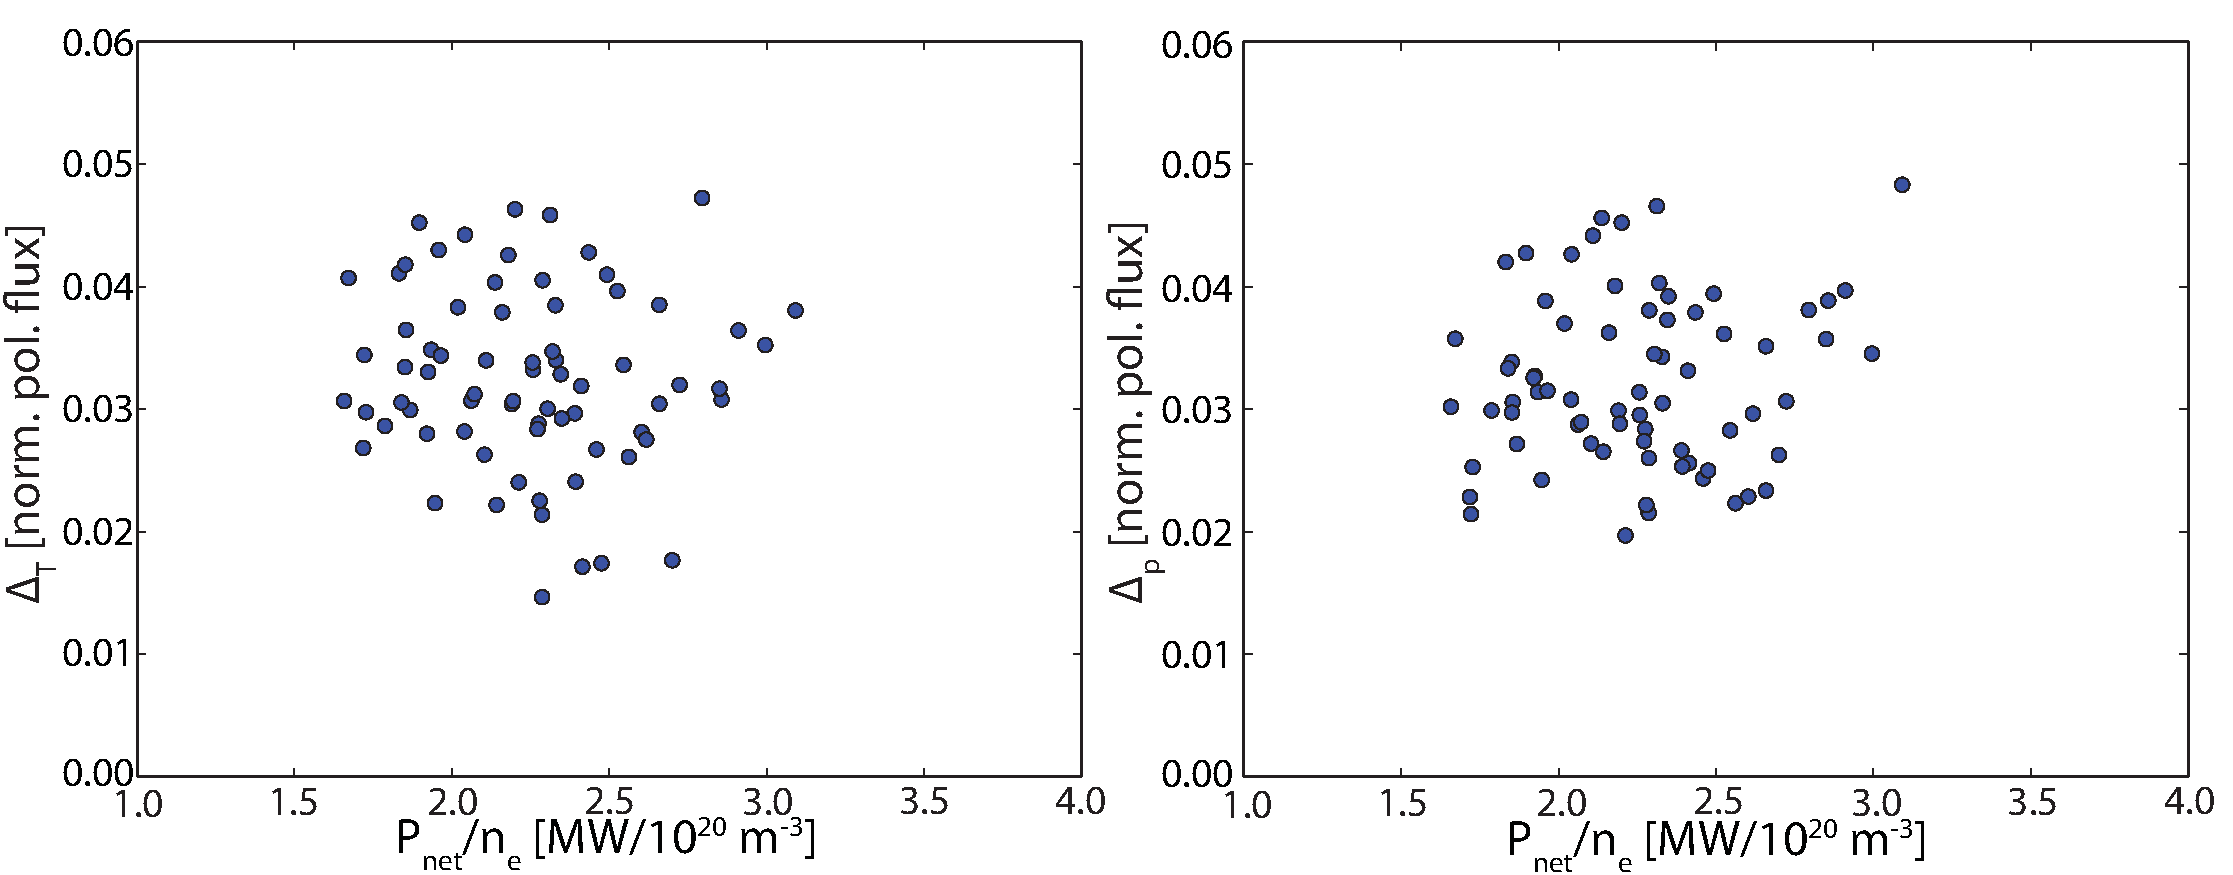
\includegraphics[width=150mm]{graphics/IModePedestal/Pnebar_widths.pdf}}{\caption[Temperature and pressure pedestal width vs. power-per-particle through the pedestal.]{Temperature (left) and pressure (right) pedestal widths versus power-per-particle, $P_{net}/\overline{n}_e$, \ie the heat flux through the pedestal.  No correlation is seen.}\label{fig:imode_Pnebar_wid}}
\end{figure}

While the constraint on the pressure pedestal from kinetic-ballooning turbulence has been the most successful in capturing the limiting physics in ELMy H-modes, a number of other theories (see \cref{sec:mod_early}) based on localized physics in the edge have been proposed, with testable trends in the pedestal width.  Of particular note are models based on a trend in poloidal gyroradius, described in \cref{subsec:mod_ionorbitloss}, operating on the assumption that ion orbit loss in the plasma edge drives the radial electric field responsible for the pedestal formation -- thus the size scale of the ion orbit sets the pedestal width.  Some experimental observations correlate well to these predictions, although these may be largely incidental due to the strong covariance between $\rho_{i,pol}$ and $\beta_{p,ped}$, and have been discounted by dedicated experiments distinguishing the two.  However, as the KBM does not appear to limit the I-mode pedestal (see \cref{subsec:imode_kbm}) gyroradius scalings remain an open possibility.  Electron temperature and pressure pedestal widths are shown against $\rho_{i,pol}$ in \cref{fig:imode_rhoipol_wid}.  Both pedestal widths appear quite insensitive to the gyroradius, although due to the correlation between $T_e$ and $I_p$ the range in $\rho_{i,pol}$ is rather limited.

Similarly, the temperature and pressure pedestal widths are shown against pedestal collisionality $\nu^*_{95}$ and edge safety factor $q_{95}$ in \cref{fig:imode_nustar_wid} and \cref{fig:imode_q95_wid}, respectively.  The collisionality may be expected to influence the pedestal width by controlling the bootstrap current in the edge, which enters into the peeling-ballooning MHD stability boundary (see \cref{sec:mod_pb}).  The safety factor is directly tied to the magnetic shear, which is locally stabilizing to MHD modes in the edge.  However, as the I-mode pedestal appears to be strongly MHD-stable, as is shown in \cref{ch:ImodeModeling}, these should have a minimal effect.  In \cref{fig:imode_nustar_wid,fig:imode_q95_wid}, no correlation between the pedestal width and either parameter is evident.

In \cref{subsec:imode_temp}, it is shown that the temperature pedestal height is strongly dependent on $P_{net}/\overline{n}_e$, effectively heating power per particle (equivalently, the heat flux through the pedestal).  Temperature and pressure pedestal widths are shown against power-per-particle in \cref{fig:imode_Pnebar_wid}.  As with the other parameters, the pedestal width is uncorrelated with the heat flux through the pedestal.

\subsection{Stiff Gradient Limits}\label{subsec:imode_wid_stiff}

\begin{figure}[t]
 \pushtooutside
 \fcapside[60mm]{\caption[I-mode pedestal temperature gradient versus pedestal temperature.]{Peak $\nabla T_e$ in the I-mode pedestal versus $T_{e,95}$.  Hotter pedestals support a steeper gradient in temperature (albeit with significant scatter), consistent with a robust temperature pedestal width.}\label{fig:imode_Te_gradT}}{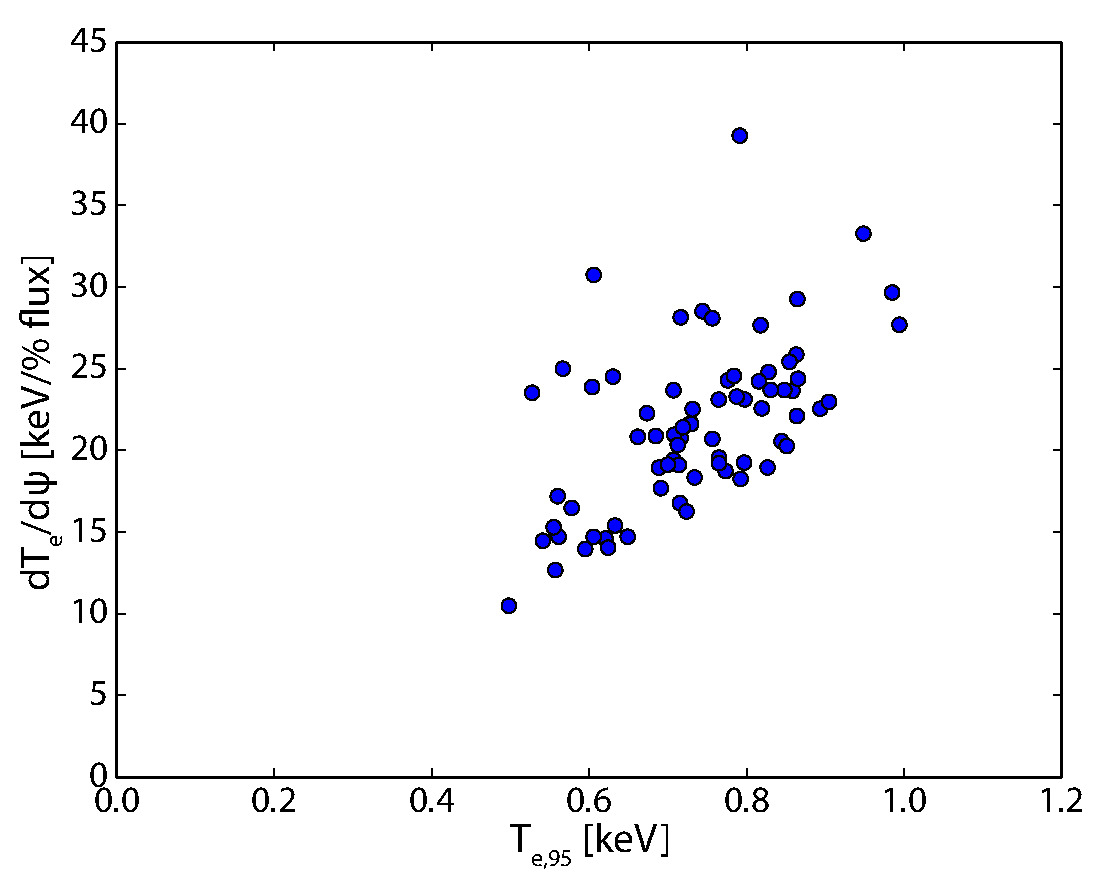
\includegraphics[width=100mm]{graphics/IModePedestal/Te95_gradT.pdf}}
\end{figure}

\begin{figure}
 \pushtooutside
 \fcapside[60mm]{\caption[I-mode pedestal pressure gradient versus pedestal pressure.]{Peak $\nabla p$ in the I-mode pedestal versus $p_{95}$.  There is a robust linear dependence between the pedestal gradient and height, consistent with a robust pedestal width.}\label{fig:imode_p_gradp}}{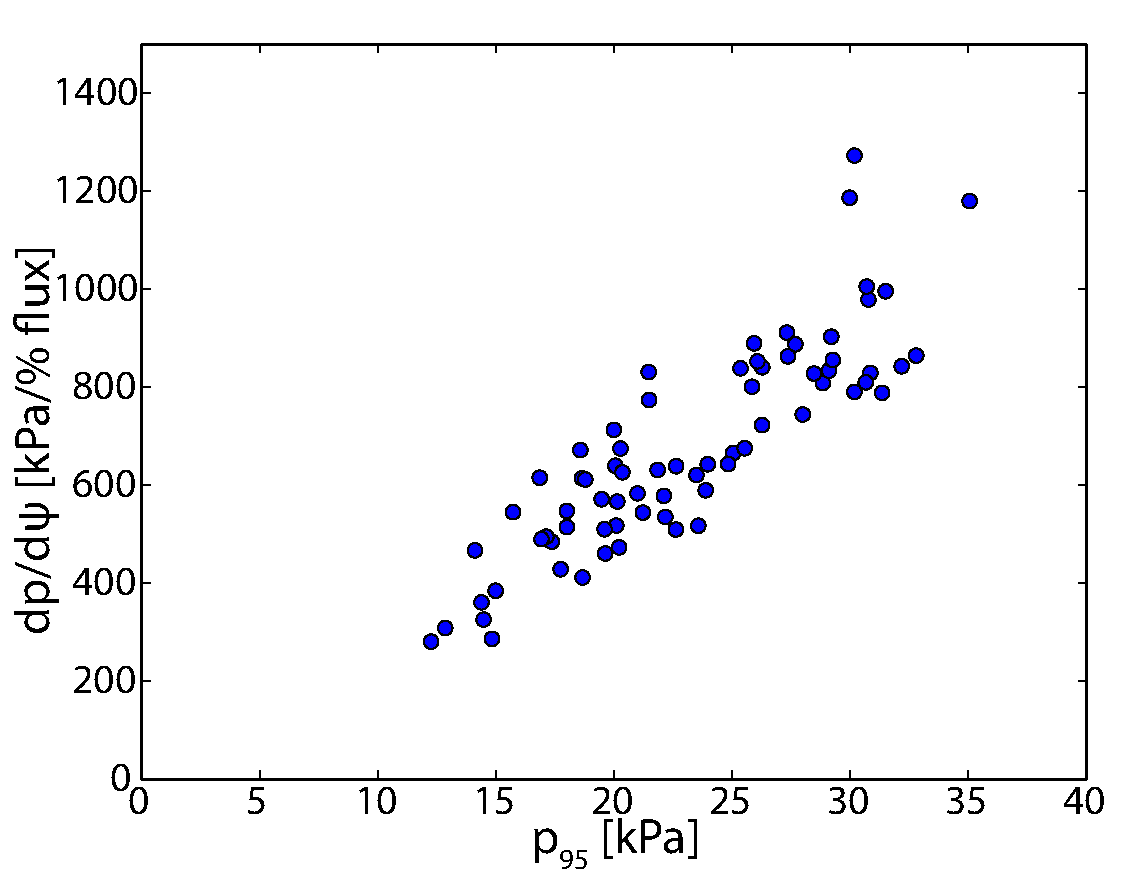
\includegraphics[width=100mm]{graphics/IModePedestal/p95_gradp_i.pdf}}
\end{figure}

In \cref{subsec:imode_kbm,subsec:imode_exp_widths}, the I-mode pedestal width (both in temperature and pressure) is shown to be insensitive to a number of pedestal parameters.  This may be examined directly by viewing the peak pedestal gradient versus its height -- to lowest approximation, $\nabla Y \sim Y/\Delta_Y$ (where $Y$ is the pedestal quantity, \ie $T_e$, $p_{tot}$).  The peak gradients in temperature and pressure are shown against the corresponding 95\%-flux values in \cref{fig:imode_Te_gradT} and \cref{fig:imode_p_gradp}, respectively.  In both cases, a linear dependence of the gradient on the pedestal-top value is observed, albeit with scatter favoring higher gradients than the linear prediction in the case of the temperature.  The pressure gradient is predicted quite well by its 95\%-flux value.  Similar behavior has been observed for the electron and ion temperatures in H-mode on AUG and DIII-D, independent of plasma shaping and evidently operating under a separate limit from the ideal-MHD constraint on the pressure pedestal \cite{Schneider2013}.  These trends are consistent with robust pedestal widths, particularly in the pressure pedestal, in I-mode.\nicesectionending

\section{Global Behavior, Performance, \& Confinement}\label{sec:imode_confinement}

The pedestal structure of the I-mode is quite desirable for a reactor scenario -- due to the strong response of the pedestal temperature to heating power, externally-applied heating power is an effective engineering control for core temperatures, and subsequently fusion reaction rates.  The high pedestal temperature, coupled to stiff core temperature profiles (such that a higher temperature supports a steeper marginally-stable $\nabla T_e$), supports very high core temperatures.  With a moderate degree of core density peaking (with typical values of $n_{e0}/\langle n_e \rangle \sim 1.1-1.3$, comparable to H-mode \cite{Greenwald2007a}), this supports comparable core and volume-averaged pressures to H-mode despite the comparatively relaxed pedestal, supporting beneficial fusion conditions in the core while avoiding stability issues in the pedestal.  Example density, temperature, and pressure profiles for I-mode and H-mode cases are shown in \cref{fig:imode_coreprofs}, illustrating the high core pressures attainable in I-mode despite the lower pedestal and reduced density.  This is reflected in \cref{fig:imode_betan_H}, showing the global-averaged normalized beta ($\langle \beta_N \rangle = \langle \beta \rangle a B_T/I_p$) versus the confinement metric $H_{98}$ in I-mode and ELMy H-mode -- I-mode reaches comparable levels of $\beta_N$ while maintaining H-mode-like $H_{98} \sim 1$ at comparable levels to ELMy H-mode, while maintaining desirable impurity confinement and ELM stability behaviors.

\begin{figure}[p]
 \pushtooutside
 \fcapside[60mm]{\caption[Density, temperature, and pressure profiles in I-mode and EDA H-mode.]{Profiles in density, temperature, and pressure for I-mode and EDA H-mode.  The H-mode case exhibits a very strong density pedestal, with a somewhat reduced temperature pedestal; the I-mode, in contrast, has a significant temperature pedestal with a relaxed density profile.  While this typically results in a reduced pedestal pressure in I-mode compared to H-mode, core profile stiffness supports very high central temperatures, such that I-mode exhibits comparable core and average pressure despite the reduced pedestal.}\label{fig:imode_coreprofs}}{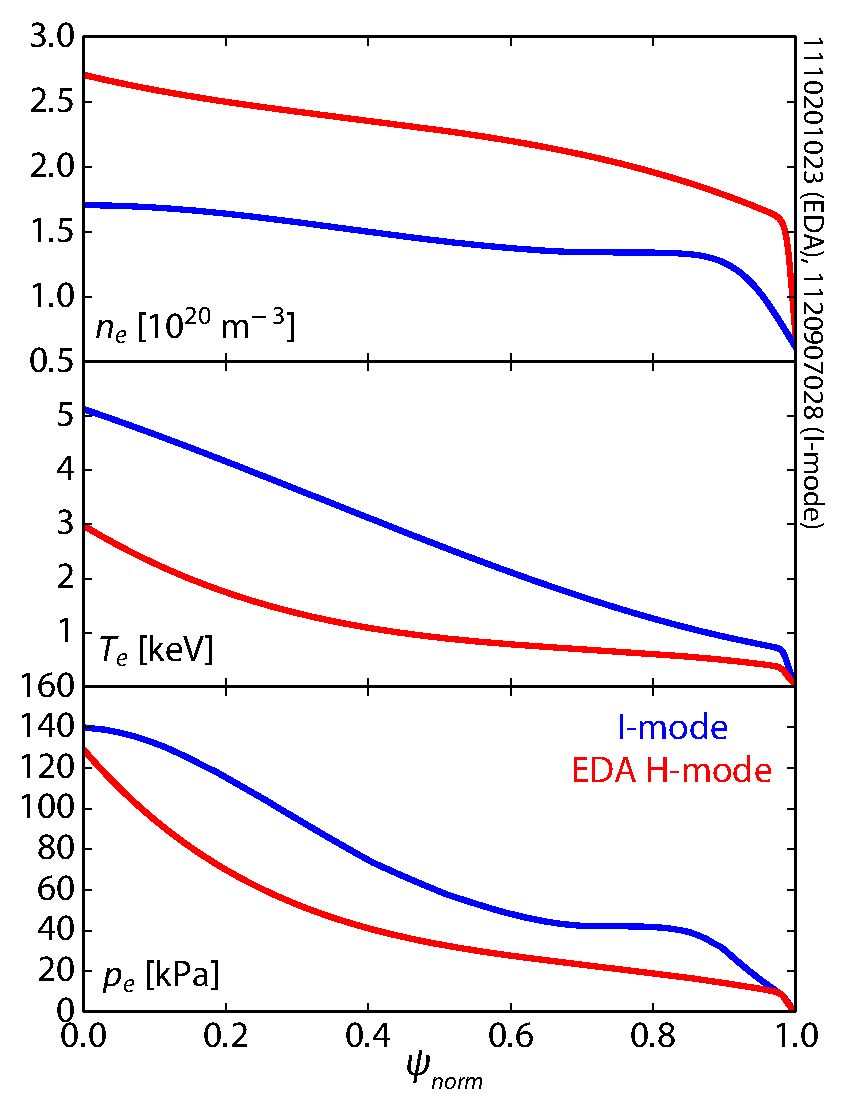
\includegraphics[width=100mm]{graphics/IModePedestal/coreprof.pdf}}
\end{figure}

\begin{figure}[p]
 \pushtooutside
 \fcapside[60mm]{\caption[Normalized beta vs. $H_{98}$ for I-mode and ELMy H-mode.]{Global normalized $\beta_N$ versus confinement factor $H_{98}$ for I-mode and ELMy H-mode.  Despite the relaxed pedestal pressure, I-modes reach comparable average pressures, while maintaining H-mode-like energy confinement.}\label{fig:imode_betan_H}}{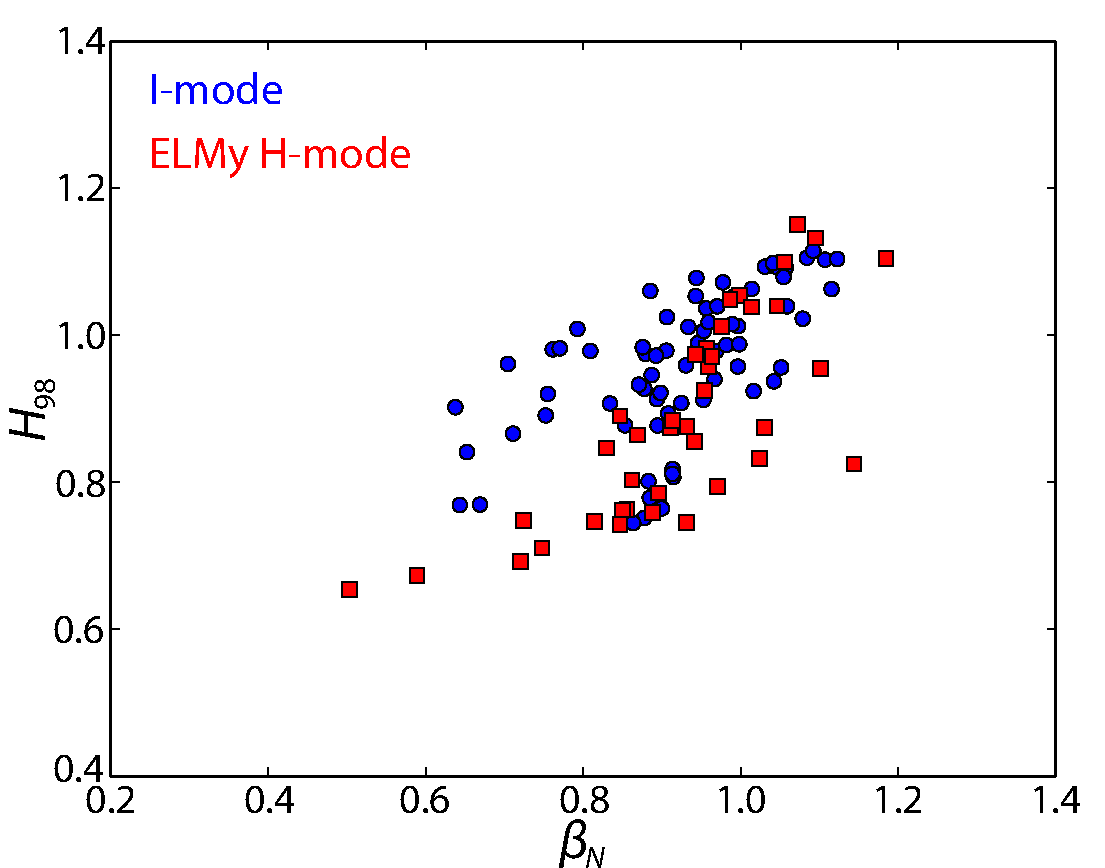
\includegraphics[width=100mm]{graphics/IModePedestal/betan_H_i_e.pdf}}
\end{figure}

\begin{figure}[p]
 \pushtooutside
 \fcapside[60mm]{\caption[I-mode stored energy vs. heating power times plasma current.]{I-mode stored energy versus the product of net heating power $P_{net}$ and plasma current $I_p$.  Based on the H-mode confinement scaling, $\tau_E$ is expected to scale linearly with $I_p$, and to show a strong degradation with heating power: $\tau_E \sim I_p \times P_{net}^{-0.7}$.  As the stored energy is given by $W \sim P_{net} \tau_E$, $W \sim I_p P_{net}^{0.3}$ is expected.  The observed linear trend indicates little-to-no degradation of $\tau_E$ in I-mode with heating power.}\label{fig:imode_PIp_W}}{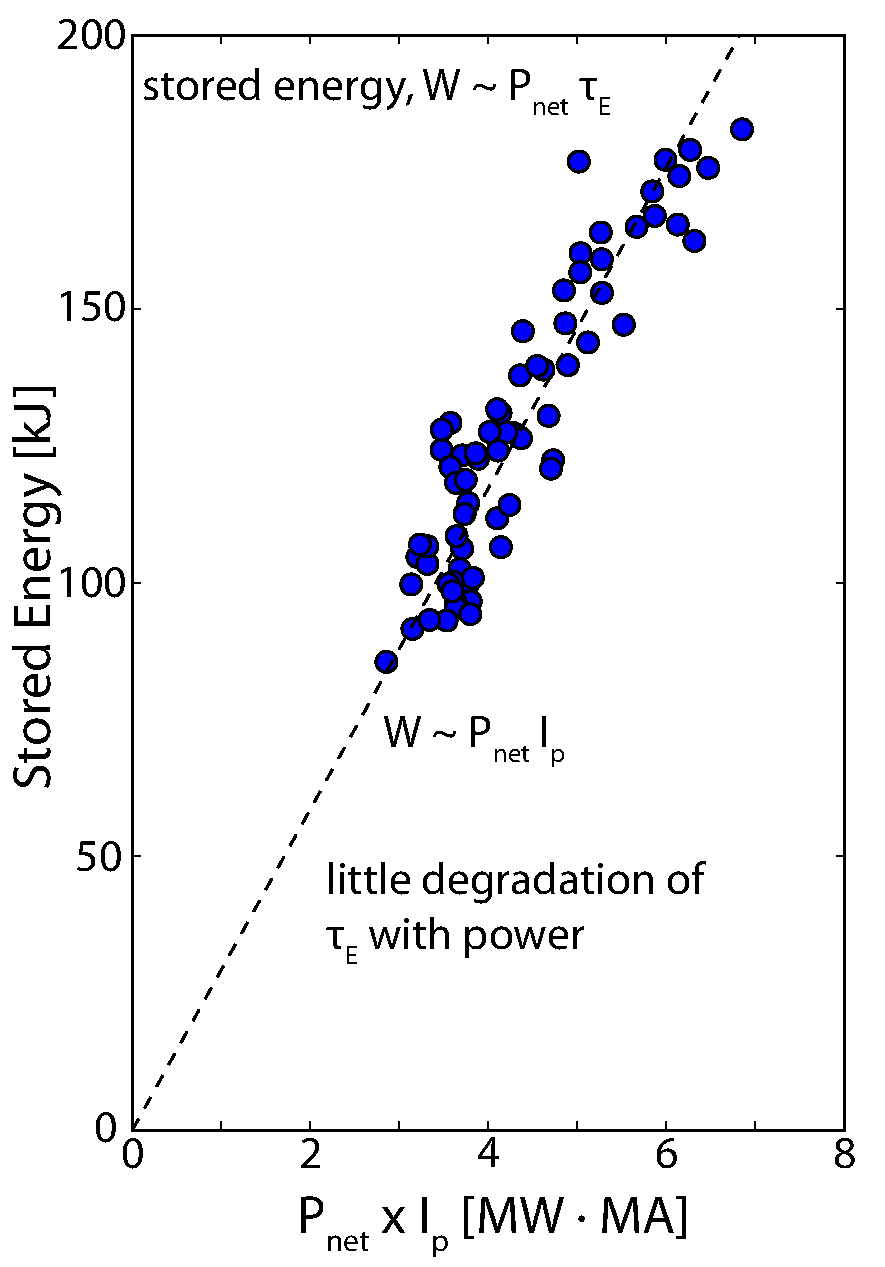
\includegraphics[width=100mm]{graphics/IModePedestal/PIp_W_scale.pdf}}
\end{figure}

\begin{figure}[p]
 \pushtooutside
 \fcapside[60mm]{\caption[Stored energy versus fueling in I-mode and H-mode.]{Plasma stored energy versus fueling, indicated by $\overline{n}_e$ in I-mode and ELMy H-mode.  I-mode stored energy increases strongly with fueling (provided sufficient power to maintain the temperature pedestal), while ELMy H-mode exhibits little trend with density -- the global stored energy and average pressure is set by the pedestal beta, which is strongly limited in ELMy H-mode.}\label{fig:imode_nebar_W}}{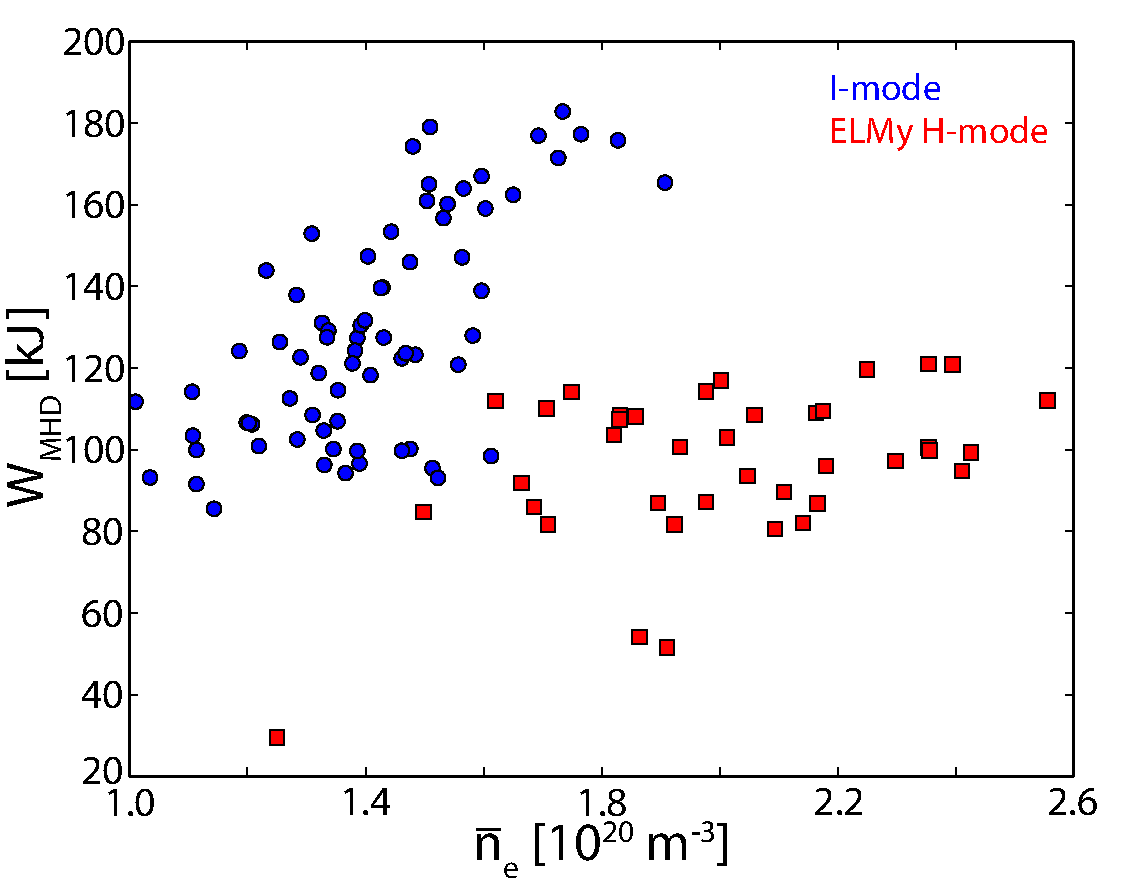
\includegraphics[width=100mm]{graphics/IModePedestal/nebar_W_i_e.pdf}}
\end{figure}

Energy confinement in I-mode also appears to lack strong degradation with heating power (\cf the $\tau_E \sim P^{-0.7}$ degradation for H-modes, as in \cref{eq:tau98}) -- a highly desirable characteristic for large devices.  This may be seen intuitively in \cref{fig:imode_PIp_W}.  The plasma stored energy trends as $W \sim P \tau_E$; from the H-mode scaling, we expect $\tau_E \sim I_p$.  The H-mode confinement scaling, then, predicts $W \sim I_p P_{net}^{0.3}$.  However, the stored energy in I-mode trends as $W \sim P_{net} I_p$, indicating that there is little or no (negative) dependence of $\tau_E$ on heating power in I-mode.  The strong dependence of the stored energy on heating power is reflected in the response of the pressure pedestal to the same, shown in \cref{fig:imode_Pnet_p95}.  The degradation of energy confinement with heating power in H-mode reflects the MHD limits on the pedestal -- increased heating power raises the ELM frequency to drive enhanced energy transport, maintaining the pedestal at the MHD limit, which in turn drives the weak increase of stored energy with increased power.  The lack of power degradation in I-mode, then, reflects the MHD stability of the pedestal.

Similarly, the beneficial response to fueling in the I-mode pedestal is reflected in global confinement, as the stored energy increases strongly with fueling levels (\cref{fig:imode_nebar_W}) -- this is particularly desirable in a burning plasma, where the alpha heating power increases with the density squared.    In contrast, ELMy H-mode stored energy is largely insensitive to fueling.  The stored energy and core $\beta_N$ is instead set by the pedestal beta, which is set predominantly by plasma shape (note, however, that there is a non-negligible effect of density vs. temperature on the core pressure, with hotter, lower-density pedestals leading to higher core pressures due to stiff temperature profiles -- however, these lower-collisionality pedestals tend to exhibit larger ELMs as well).

\subsection{Confinement Scaling Laws}\label{subsec:imode_powerlaws}

Due to the complexity inherent in modeling global energy transport from first-principles physics, it is common to establish empirical scaling laws for energy confinement using a power-law fit to large datasets.  For example, the ITER89 \cite{Yushmanov1990} and ITER98 \cite{ITER1999} scalings utilized an extensive multi-machine database \cite{Christiansen1992} for L-mode and H-mode confinement.  In particular the ITER98y2 scaling (see \cref{eq:tau98}) is a commonly-used baseline for high-performance regimes, particularly in terms of the normalized $H_{98}$ (\cref{eq:H98}).  However, as the ITER98y2 scaling was constructed predominantly with type-I ELMy H-modes (as these customarily are the highest-performance H-modes on most tokamaks), and as such implicitly includes the physics of ELM-limited pedestals.  For example, the power-law fit in ITER98y2 includes a strong degradation of confinement with heating power, $\tau_E \sim P^{-0.7}$.  This is consistent with the observed weak response of ELMing pedestals with heating power \cite{Snyder2007}, with increased power instead raising the ELM frequency to maintain consistent ELM-driven heat transport.

In light of the substantially different physics of the I-mode pedestal and energy confinement compared to H-modes, it is useful to construct a power-law confinement fit using I-mode data.  It is strongly emphasized that such a fit would be only preliminary, as fits using data from a single machine lack the range of parameter values needed to extrapolate to devices of different size.  I-mode energy confinement times are fitted in a least-squares sense to the general form

\begin{equation}\label{eq:taufit}
 \tau_{I-mode} = C \; I_p^{\alpha_{I_p}} \; B_T^{\alpha_{B_T}} \; \overline{n}_e^{\alpha_{n_e}} \; R^{\alpha_R} \; \varepsilon^{\alpha_\varepsilon} \; \kappa^{\alpha_\kappa} \; P_{loss}^{\alpha_P}
\end{equation}

\noindent to find free exponents $\alpha_j$ for plasma current $I_p$ in $\si{\mega\ampere}$, toroidal field $B_T$ in $\si{\tesla}$, line-averaged density $\overline{n}_e$ in $\SI{e20}{\per\meter\cubed}$, major radius $R$ in $\si{\meter}$, inverse aspect ratio $\varepsilon$, elongation $\kappa$, and loss power $P_{loss}$ in $\si{\mega\watt}$ (see \cref{eq:ploss}).  To extend the quantity of data and range of parameters available for this assay, the high-resolution pedestal data used in the bulk of this thesis is supplemented by older I-mode datasets containing both reversed-field LSN and forward-field USN I-mode cases.  Although these data lack the high-resolution edge data necessary for pedestal structure and stability studies, they are nevertheless suitable for scalings based on global parameters.  Although the net power $P_{net}$ (see \cref{eq:pnet}) has been demonstrated to be the more suitable parameter, rather than $P_{loss}$ \cite{Hughes2002}, these older data contain inconsistent measurements of the radiated power, necessitating the use of loss power in its stead.  However, the radiated power is typically a fairly small fraction of the total power in I-mode ($P_{rad} < \SI{900}{\kilo\watt}$, $P_{rad}/P_{tot} < 20\%$), and in any case this is consistent with previous confinement scaling studies, so the use of $P_{loss}$ is sufficient for a first-pass examination of confinement.

\begin{table*}
 \pushtooutside
 \ttabbox{\caption[Parameters for power-law scalings of I-mode energy confinement time.]{Parameters for power-law scalings of the I-mode energy confinement time $\tau_E$, along with $r^2$ coefficients of determination for the fit.  Blank entries indicate parameters that were omitted from that fit.  Note that fit \#5 utilized a fixed $R^2 \sqrt{\varepsilon}$ size dependence rather than taking the size to be a free fitting parameter.  Parameters are in the given units: $I_p$ in $\si{\mega\ampere}$, $B_T$ in $\si{\tesla}$, $\overline{n}_e$ in $\SI{e20}{\per\meter\cubed}$, $R$ in $\si{\meter}$, and $P_{loss}$ in $\si{\mega\watt}$.  Elongation $\kappa$ and aspect ratio $\varepsilon$ are dimensionless.}\label{tab:imode_confinement}}{
 \begin{tabular}{cccccc}
  \toprule
  & \#1 & \#2 & \#3 & \#4 & \#5 \\
  \midrule
  $C$ & $0.040 \pm 0.066$ & $0.007 \pm 0.002$ & $0.014 \pm 0.002$ & $0.014 \pm 0.002$ & $0.056 \pm 0.008$ \\
  $I_p$ & $0.686 \pm 0.074$ & $0.696 \pm 0.073$ & $0.685 \pm 0.076$ & $0.692 \pm 0.073$ & $0.676 \pm 0.077$ \\
  $B_T$ & $0.698 \pm 0.075$ & $0.697 \pm 0.071$ & $0.768 \pm 0.072$ & $0.773 \pm 0.071$ & $0.767 \pm 0.072$ \\
  $\overline{n}_e$ & $-0.077 \pm 0.055$ & $-0.050 \pm 0.048$ & $0.017 \pm 0.048$ & & $0.006 \pm 0.048$ \\
  $R$ & $4.219 \pm 4.623$ & & & & $2^*$ \\
  $\varepsilon$ & $0.127 \pm 1.144$ & & & & $0.5^*$ \\
  $\kappa$ & $1.686 \pm 0.398$ & $1.501 \pm 0.350$ & & & \\
  $P_{loss}$ & $-0.197 \pm 0.048$ & $-0.220 \pm 0.043$ & $-0.286 \pm 0.042$ & $-0.281 \pm 0.039$ & $-0.275 \pm 0.042$ \\
  $r^2$ & $0.713$ & $0.711$ & $0.685$ & $0.684$ & $0.683$ \\
  \bottomrule
 \end{tabular}
 }
\end{table*}

Results from a number of scaling studies are shown in \cref{tab:imode_confinement}, containing the values and standard deviations for each exponent value, the scale factor $C$, and the $r^2$ coefficient of determination.  We begin with the full parameter list used in the ITER98y2 scaling, shown as fit \#1 in \cref{tab:imode_confinement}, with results shown in \cref{fig:imode_tauE_1}.  However, it is immediately obvious that the size scalings, dependent on major radius $R$ and inverse aspect ratio $\varepsilon$, are not properly captured (denoted by the extreme errorbars on these parameters).  This is to be expected -- absent meaningful variation in $R$ and $\varepsilon$ in the dataset (which requires multiple machines to produce) these parameters are not well-constrained, and result \#1 is over-fitted.  

For simplicity, we reduce our consideration to an effective single-machine scaling, omitting these parameters (indicated by blank entries in \cref{tab:imode_confinement}).  Under this fit, shown as \#2 in \cref{tab:imode_confinement}, the power applied to the elongation $\kappa$ is elevated compared to that expected from the ITER98y2 scaling, with the relatively large deviation expected from the somewhat restricted range of shapes found in these studies.  Omitting this fitting parameter results in a minimum-complexity fit,

\begin{equation}\label{eq:tauE_fit_3}
 \tau_{I-mode} = 0.014 \times I_p^{0.685} \; B_T^{0.768} \; \overline{n}_e^{0.017} \; P_{loss}^{-0.286}
\end{equation}

\noindent with a coefficient of determination of $r^2 = 0.685$ (also shown as \#3 in \cref{tab:imode_confinement}).  The correspondence between experimenal $\tau_E$ and the modeled confinement time is shown in \cref{fig:imode_tauE_3}.  The density dependence in $\tau_E$ is quite weak, and may be omitted (fit \#4) with minimal alteration to the result; however, this may not capture effects on the transport at higher Greenwald fraction, and requires additional experiments.  Both fits capture the weak degradation of $\tau_E$ with input power, compared to standard L- or H-mode, consistent with observations of the pedestal and global stored energy.  The strong depedence of $\tau_E$ on current is similar to that expected for H-modes, while the $B_T$ dependence is stronger; notably, the H-mode threshold power is strongly dependent on magnetic field (see \cref{eq:pthres}), this may reflect the fact that I-modes are bounded above by the transition to H-mode, allowing higher confinement and more aggressive pedestals at stronger $B_T$ simply by suppressing the I-H transition.

\begin{figure}[t]
 \pushtooutside
 \begin{floatrow}
  \ffigbox[\FBwidth]{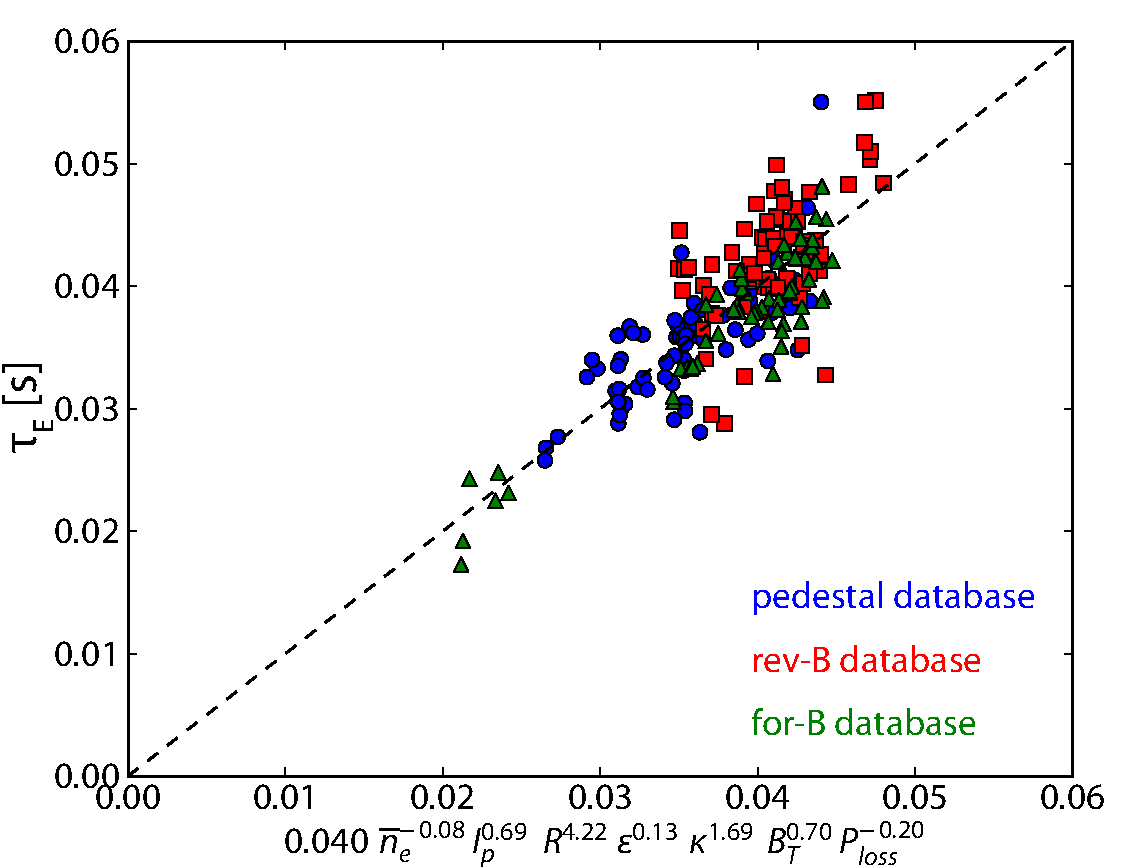
\includegraphics[width=75mm]{graphics/IModePedestal/tauE_1_Ploss_sep.pdf}}{\caption[Power-law fit to I-mode $\tau_E$ with full parameter set.]{Power-law fit for I-mode energy confinement time $\tau_E$, fitted using the full ITER98y2 parameter set (fit \#1 in \cref{tab:imode_confinement}).  Both the high-resolution pedestal database and older reversed-field LSN and forward-field USN I-mode databases are used.  While the fit is generally good, lack of variation in certain parameters -- particularly the size parameters $R$ and $\varepsilon$ (as expected for a single-machine scaling), and elongation $\kappa$ mean that the true variation with these parameters is not accurately captured.  However, the expected weak degradation of $\tau_E$ with heating power is captured.}\label{fig:imode_tauE_1}}
  \ffigbox[\FBwidth]{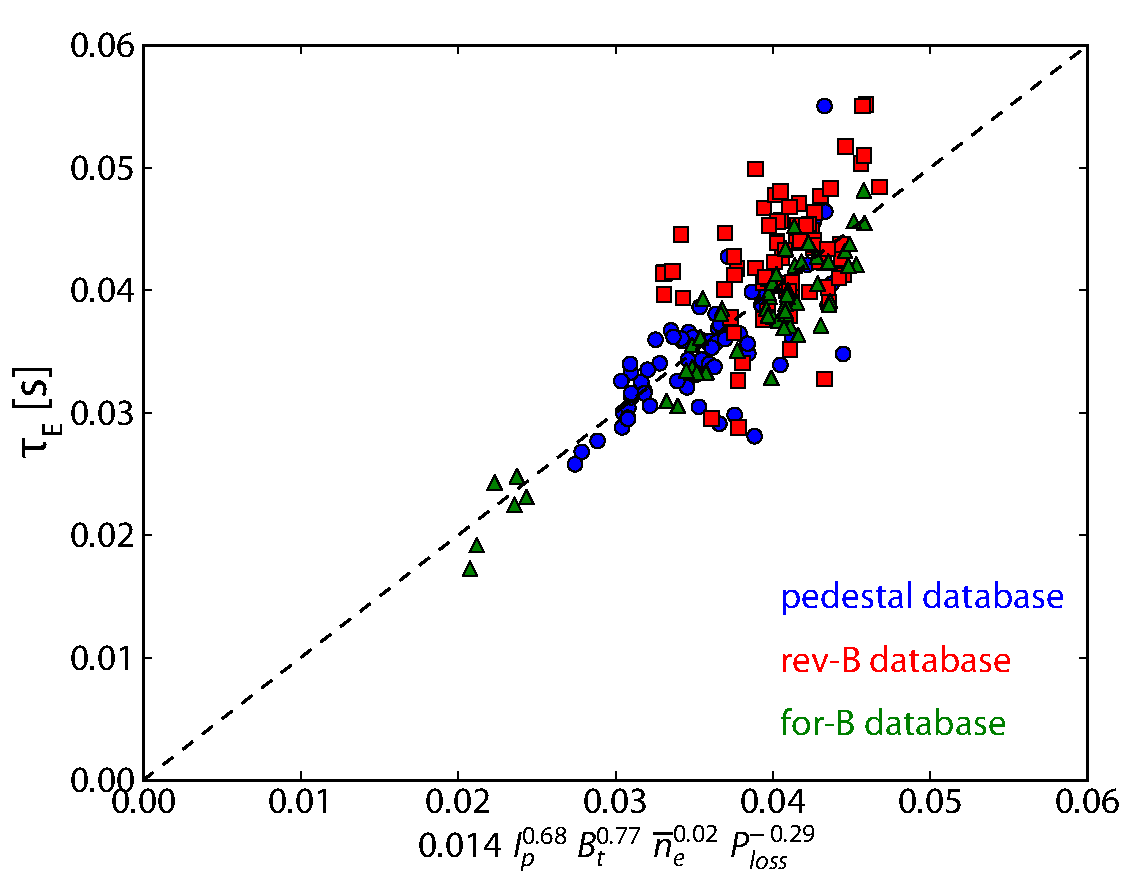
\includegraphics[width=75mm]{graphics/IModePedestal/tauE_3_Ploss_sep.pdf}}{\caption[Power-law fit to I-mode $\tau_E$, with poorly-fitted parameters excluded.]{Power-law fit for I-mode energy confinement time $\tau_E$, fitted with the size parameters $R$ and $\varepsilon$, and elongation $\kappa$ excluded due to the lack of variation in these variables in the available data (fit \#3 in \cref{tab:imode_confinement}).  Both the high-resolution pedestal database and older reversed-field LSN and forward-field USN I-mode databases are used.  This represents the minimum-complexity fit for I-modes on C-Mod, capturing the essential dependences on current, field, and fueling, and notably the weak degradation of confinement with heating power.}\label{fig:imode_tauE_3}}
 \end{floatrow}
\end{figure}

\begin{figure}[t]
 \pushtooutside
 \begin{floatrow}
  \ffigbox[\FBwidth]{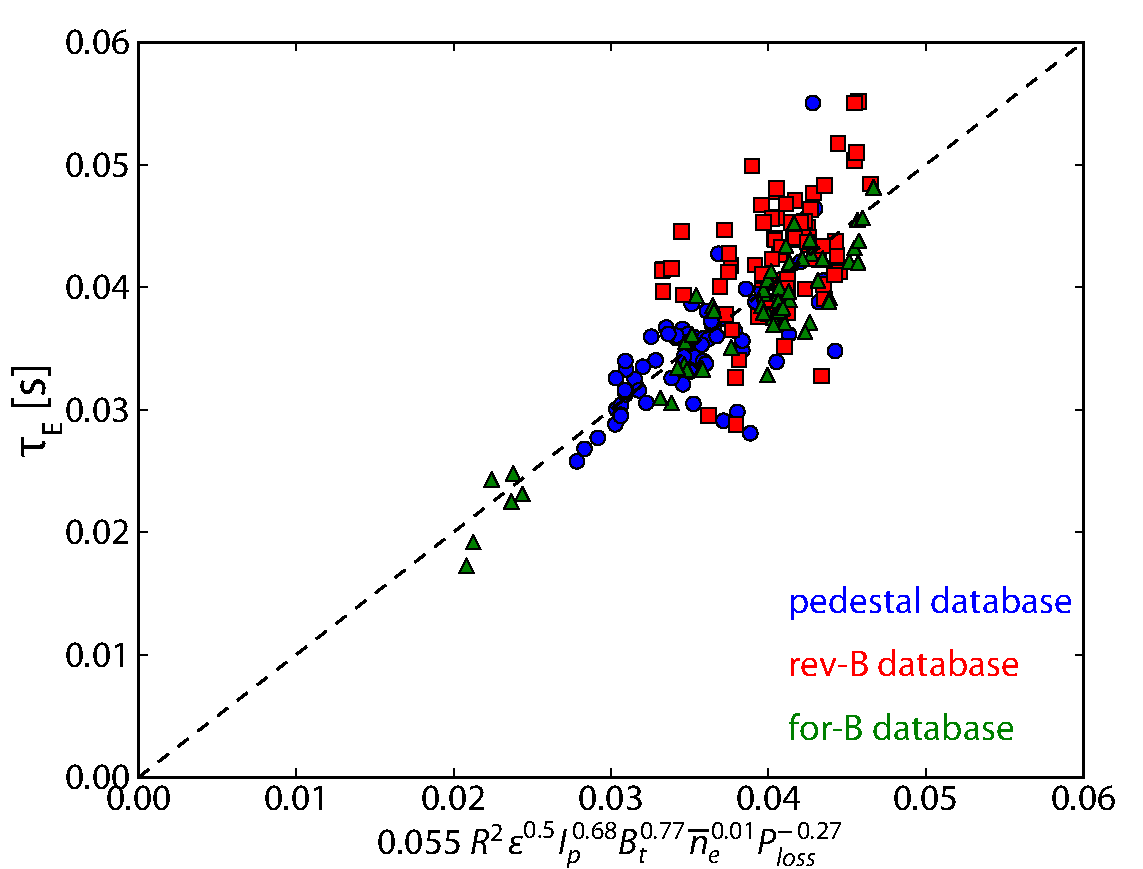
\includegraphics[width=75mm]{graphics/IModePedestal/tauE_6_Ploss_sep.pdf}}{\caption[Power-law fit to I-mode $\tau_E$, with fixed $R^2 \sqrt{\varepsilon}$ size scaling.]{Power-law fit to I-mode energy confinement time $\tau_E$, with the \emph{ansatz} of an $R^2 \sqrt{\varepsilon}$ size scaling fixed (fit \#5 in \cref{tab:imode_confinement}).  Both the high-resolution pedestal database and older reversed-field LSN and forward-field USN I-mode databases are used.  Note the expected weak degradation of $\tau_E$ with heating power.}\label{fig:imode_tauE_6}}
  \ffigbox[\FBwidth]{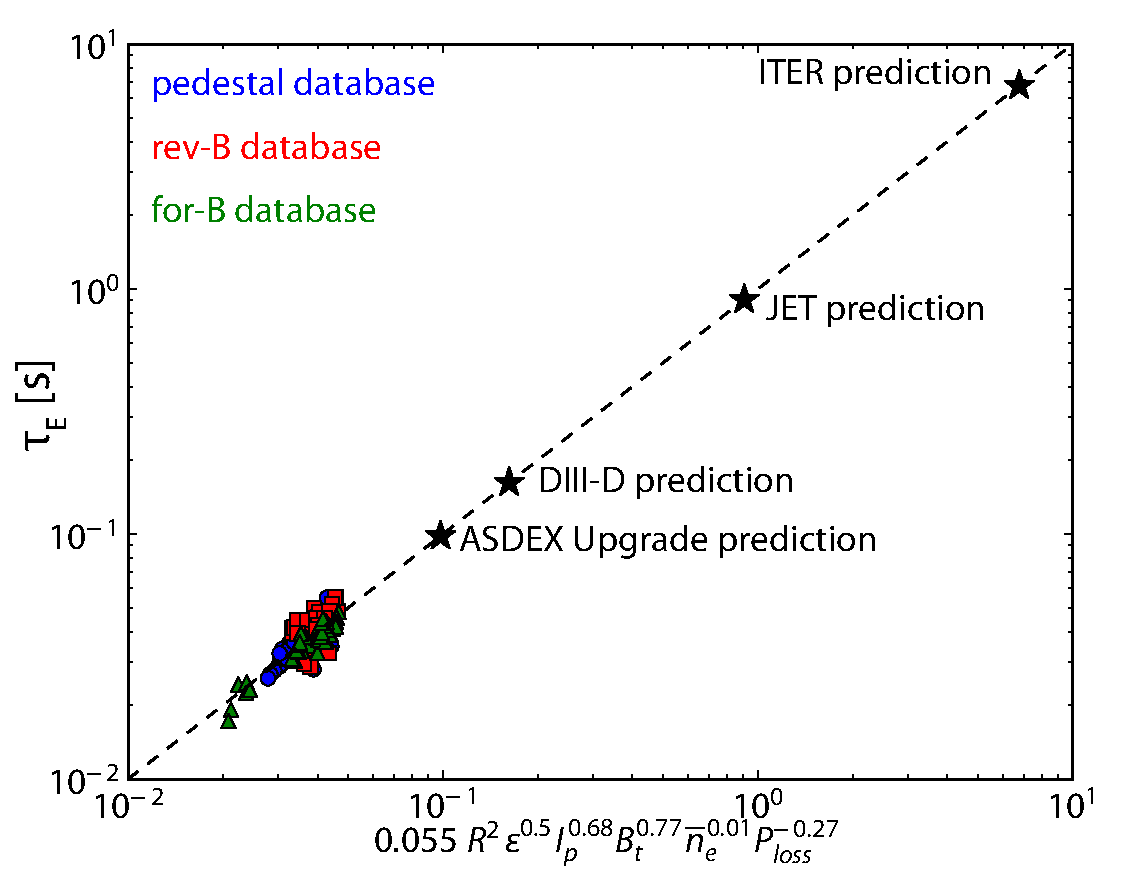
\includegraphics[width=75mm]{graphics/IModePedestal/tauE_6_Ploss_extrap.pdf}}{\caption[Power-law fit to I-mode $\tau_E$ extrapolated to larger devices.]{Modeled energy confinement time $\tau_E$ with the fixed $R^2 \sqrt{\varepsilon}$ size scaling (fit \#5 in \cref{tab:imode_confinement}), extrapolated to DIII-D, ASDEX Upgrade, JET, and ITER.  Modeled energy confinement times are competitive with H-modes, both the measured $\tau_E$ for existing machines and the expected ITER98y2 prediction for ITER H-modes.}\label{fig:imode_tauE_extrap}}
 \end{floatrow}
\end{figure}

As an illustrative exercise, we restore a fixed size dependence of the form $R^2 \sqrt{\varepsilon}$ (as is found in ITER98y2) to the fit, shown as \#5 in \cref{tab:imode_confinement}, with the correspondence to experimental $\tau_E$ shown in \cref{fig:imode_tauE_6}.  This enables extrapolation of the result to larger devices, with example predictions for DIII-D, ASDEX Upgrade, JET, and ITER shown in \cref{fig:imode_tauE_extrap}.  Due to the weakened power degradation ($\tau_E \sim P^{-0.28}$), I-mode operation on ITER (in the putative $Q=10$ scenario with $\SI{100}{\mega\watt}$ of alpha heating) projects to a $\sim \SI{8}{\second}$ energy confinement time, well in excess of the expected $\tau_E \sim \SI{2.5}{\second}$ for H-mode.

Again, we emphasize that single-machine scalings are of limited reliability for extrapolative purposes.  However, this illustrates the potential gains in performance in the application of I-mode to larger devices, while correctly capturing the observed physics in I-mode (\eg the degradation in $\tau_E$ is, to within uncertainty, consistent with the observed strong dependence of the stored energy and pedestal pressure on heating power).  However, it is notable that preliminary results in I-mode experiments on ASDEX Upgrade observed energy confinement times in the range of $0.07-\SI{0.1}{\second}$, consistent with the predictions of the I-mode model in the corresponding parameter range, although detailed analysis of these shots has not been performed.\nicesectionending

%\begin{figure}
% \pushtooutside
% \fcapside[60mm]{\caption[Power-law fit to I-mode $\tau_E$ with full parameter set.]{Power-law fit for I-mode energy confinement time $\tau_E$, fitted using the full ITER98y2 parameter set (fit \#1 in \cref{tab:imode_confinement}).  Both the high-resolution pedestal database and older reversed-field LSN and forward-field USN I-mode databases are used.  While the fit is generally good, lack of variation in certain parameters -- particularly the size parameters $R$ and $\varepsilon$ (as expected for a single-machine scaling), and elongation $\kappa$ mean that the true variation with these parameters is not accurately captured.  However, the expected weak degradation of $\tau_E$ with heating power is captured.}\label{fig:imode_tauE_1}}{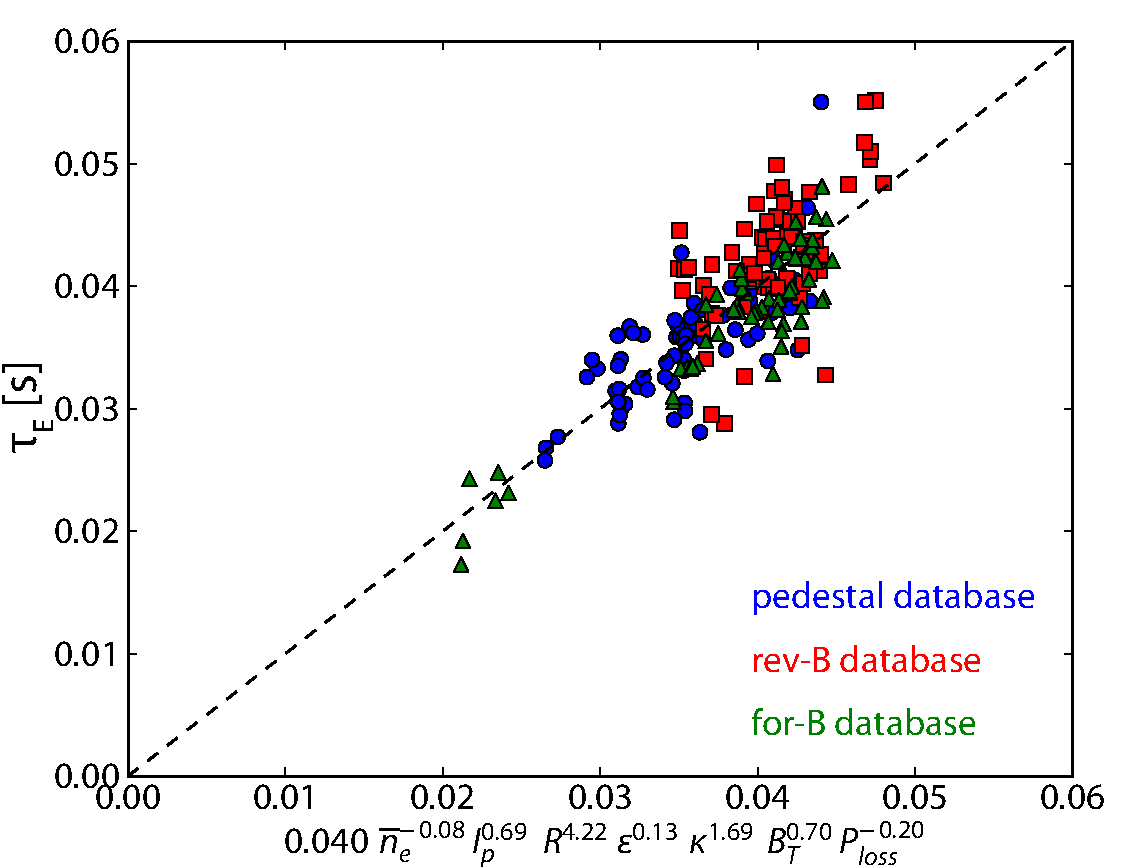
\includegraphics[width=100mm]{graphics/IModePedestal/tauE_1_Ploss_sep.pdf}}
%\end{figure}

%\begin{figure}
% \pushtooutside
% \fcapside[60mm]{\caption[Power-law fit to I-mode $\tau_E$, with poorly-fitted parameters excluded.]{Power-law fit for I-mode energy confinement time $\tau_E$, fitted with the size parameters $R$ and $\varepsilon$, and elongation $\kappa$ excluded due to the lack of variation in these variables in the available data (fit \#3 in \cref{tab:imode_confinement}).  Both the high-resolution pedestal database and older reversed-field LSN and forward-field USN I-mode databases are used.}\label{fig:imode_tauE_3}}{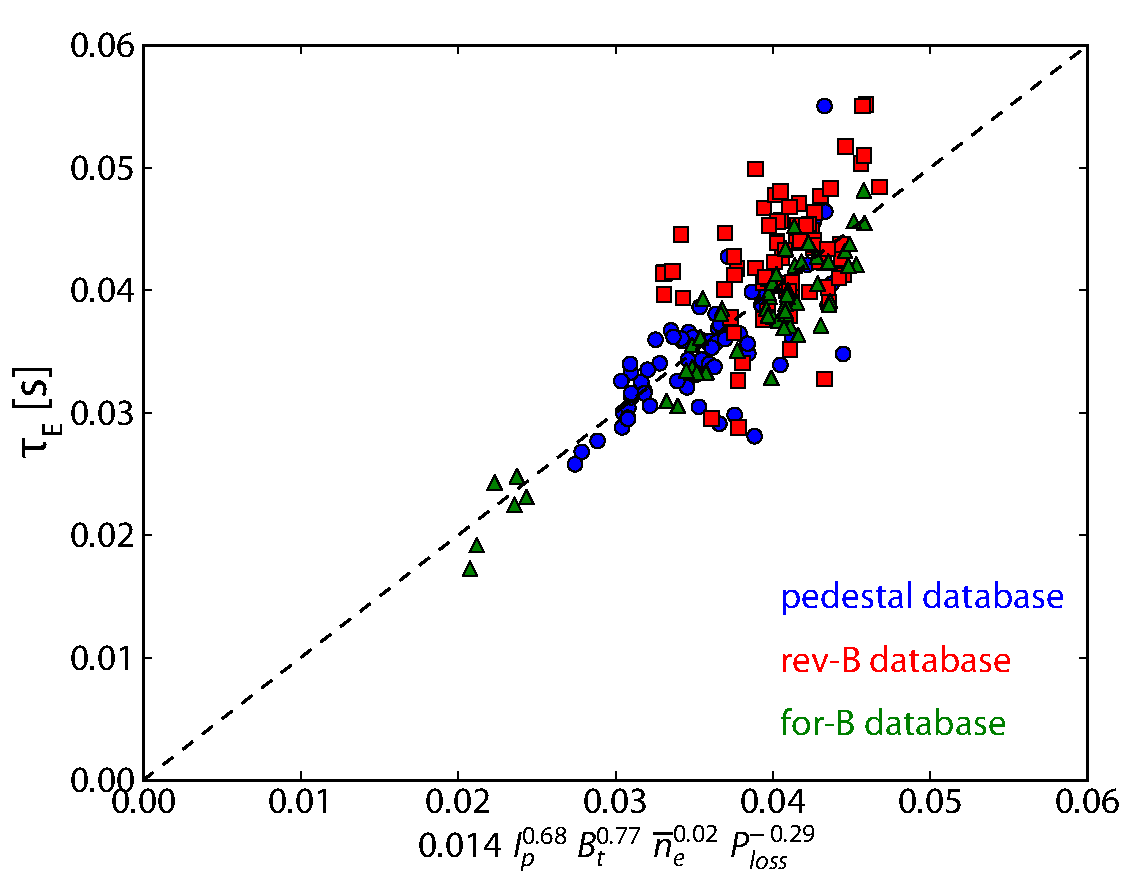
\includegraphics[width=100mm]{graphics/IModePedestal/tauE_3_Ploss_sep.pdf}}
%\end{figure}

%\begin{figure}
% \pushtooutside
% \fcapside[60mm]{\caption[Power-law fit to I-mode $\tau_E$, with fixed $R^2 \sqrt{\varepsilon}$ size scaling.]{Power-law fit to I-mode energy confinement time $\tau_E$, with the \emph{ansatz} of an $R^2 \sqrt{\varepsilon}$ size scaling fixed (fit \#5 in \cref{tab:imode_confinement}).  Both the high-resolution pedestal database and older reversed-field LSN and forward-field USN I-mode databases are used.  Note the expected weak degradation of $\tau_E$ with heating power.}\label{fig:imode_tauE_6}}{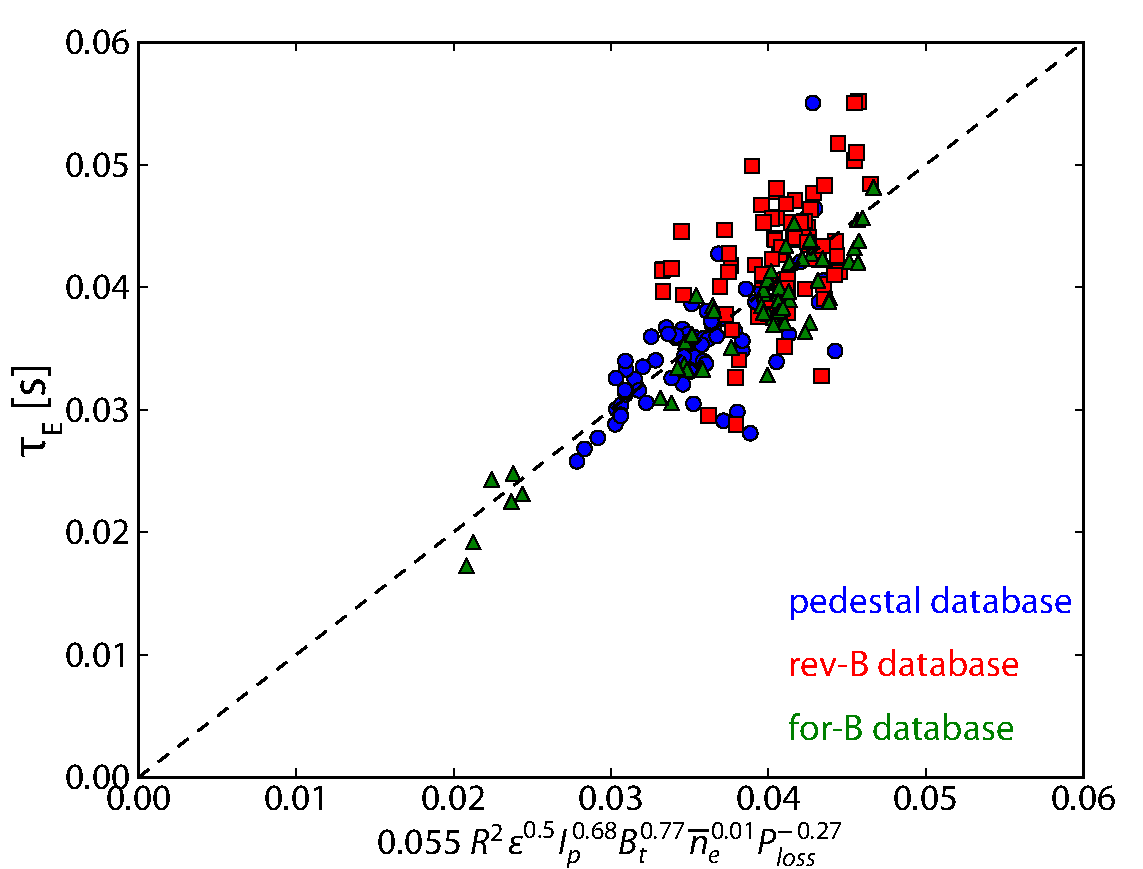
\includegraphics[width=100mm]{graphics/IModePedestal/tauE_6_Ploss_sep.pdf}}
%\end{figure}
%
%\begin{figure}
% \pushtooutside
% \fcapside[60mm]{\caption[Power-law fit to I-mode $\tau_E$ extrapolated to larger devices.]{Modeled energy confinement time $\tau_E$ with the fixed $R^2 \sqrt{\varepsilon}$ size scaling (fit \#5 in \cref{tab:imode_confinement}, extrapolated to DIII-D, ASDEX Upgrade, JET, and ITER.  Modeled energy confinement times are competitive with H-modes, both the measured $\tau_E$ for existing machines and the expected ITER98y2 prediction for ITER H-modes.}\label{fig:imode_tauE_extrap}}{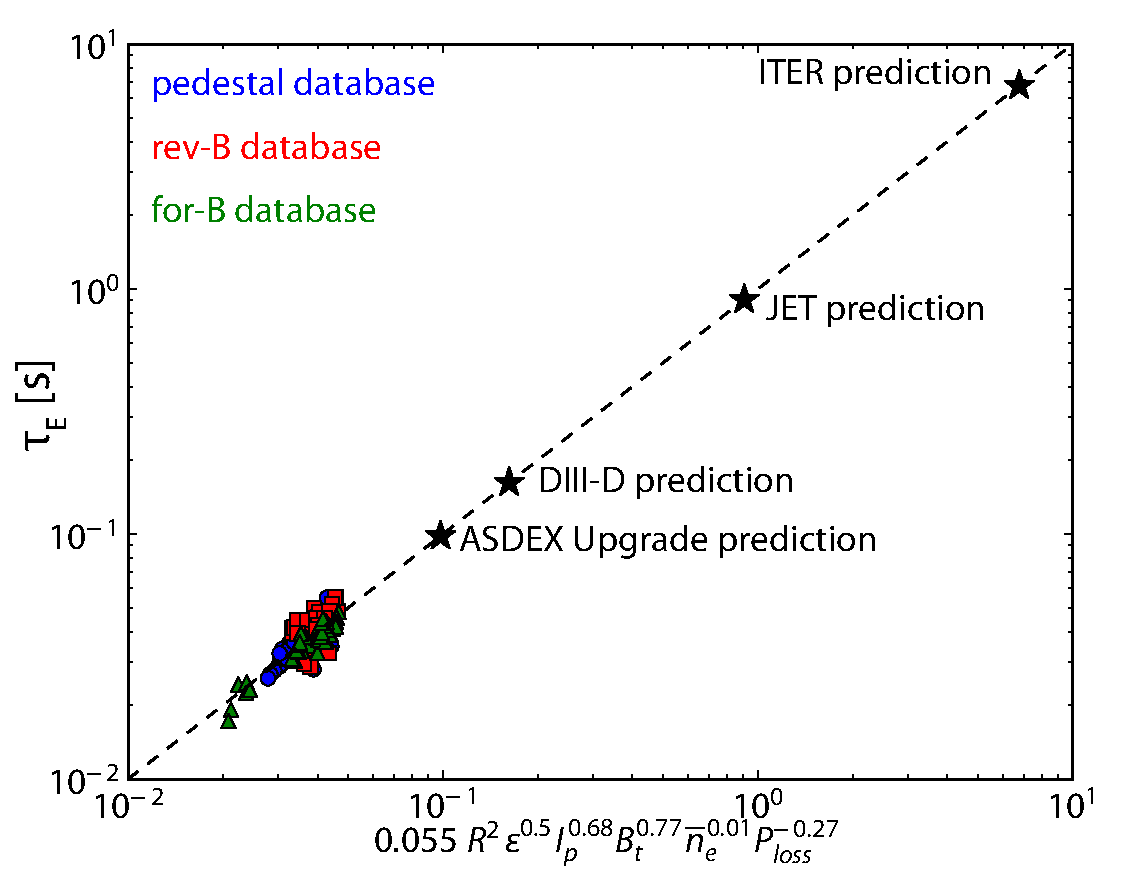
\includegraphics[width=100mm]{graphics/IModePedestal/tauE_6_Ploss_extrap.pdf}}
%\end{figure}

\section{Summary \& Discussion}\label{sec:imode_ped_conclusions}

%I-mode is a promising alternate regime for high-confinement operation on ITER- and reactor-scale devices, characterized by its apparent decoupling of the energy and particle transport channels.\gnote{could probably trim out first two paragraphs...}  I-mode operation generates a high-temperature, low-collisionality pedestal (naturally operating near ITER-target $\nu^*_{95}$ and $q_{95}$, as shown in \cref{fig:imode_q_nustar}) while maintaining an L-mode-like density profile -- this allows H-mode levels of energy confinement with L-mode levels of impurity transport, desirable for stationary operation with high-$Z$ metal wall materials.  I-mode also appears to be free of large ELMs, avoiding the large pulsed heat loads anticipated for uncontrolled ELMy H-modes in ITER-scale devices without the need for externally-applied engineering solutions for ELM mitigation/suppression (see \cref{subsec:hcr_elmy_control}).

Due to the strong influence of the pedestal structure on global confinement and performance, as well as on stability against large ELM events, a firm understanding of the pedestal is essential for the extrapolation of I-mode operation to larger devices.  Empirical observations of the I-mode pedestal and global performance provide an intuitive picture of I-mode pedestal structure and stability in comparison to conventional high-confinement regimes (particularly the canonical type-I ELMy H-mode), consistent with beneficial H-mode-like behaviors in energy confinement modified by the enhanced particle transport in I-mode.

The pedestal temperature is found to scale strongly with plasma current, $T_{e,95} \sim I_p$, comparable to that found in H-mode (\cf the results in \cref{ch:Elmy}).  Notably, the I-mode temperature pedestal height is found to scale strongly with heating power per particle, $T_{e,95} \sim P_{net}/\overline{n}_e$, in contrast to the minimal positive effect of heating power on the temperature pedestal in ELMy H-mode (note that the temperature pedestal in transport-limited EDA H-modes exhibit a positive trend with heating power somewhat weaker than in I-mode).    Similarly, the pressure pedestal height scales strongly with heating power, $p_{95} \sim n_{e,95} T_{e,95} \sim P_{net}$, significantly more strongly than in H-mode.  In contrast, the density profile is set externally by operator fueling control independent of physics limits, due to the L-mode-like particle confinement -- a highly desirable result for fueling scenarios on ITER.  Given sufficient power to maintain a given value of $P_{net}/\overline{n}_e$, temperature pedestals are matched across a range of fueling levels (\cref{fig:imode_fuelingprofiles}).  Heating power and fueling are thus two largely-independent ``knobs'' for operator control of pedestal profiles, in contrast to both ELMy H-modes (which exhibit an inverse relationship between density and temperature due to the limit on $\beta_{p,ped}$ imposed by MHD stability) and EDA H-modes (in which the pedestal density is locked to a value set by the current due to the interplay between particle-pinch and transport effects).

The pedestal width in I-mode does not appear to trend strongly with any of the examined physics parameters.  No dependence on $\beta_{p,ped}$ is seen, suggesting that the I-mode pedestal is not limited by KBM turbulence; moreover, the I-mode pedestal is consistently wider than predicted from the KBM width constraint used in the EPED model for ELMy H-mode.  Similarly, no width dependence is seen on the poloidal gyroradius, collisionality, safety factor/magnetic shear, or heat flux through the pedestal.  Both the temperature and pressure pedestal width appear to be robust across the observed range in I-mode pedestals, such that the peak gradient in each is linearly dependent on the pedestal-top value.  However, it should be noted that the pressure gradient is consistently shallower than that found in H-mode due to the flat density profile, and does not exhibit the trend with plasma current expected for an MHD-limited pedestal, consistent with the observed lack of ELMs.

Although the I-mode exhibits a more relaxed pressure pedestal than found in H-mode, the comparatively higher temperature pedestal supports steep core temperature profiles, reaching significant core and average pressure provided a moderate degree of density peaking.  Thus, I-mode is capable of reaching competitive levels of global confinement (both in terms of averaged pressure, $\beta_N$, and normalized confinement time $H_{98} \sim 1$) with H-mode, while the relaxed pedestal provides beneficial stability and particle-confinement properties.  It should be noted that the strongly reactive region of the plasma for fusion events (where $\langle \sigma v \rangle \sim T_i^2$, or $R_{fusion} \sim p^2$) is largely restricted to where the plasma temperature is greater than $\sim \SI{4}{\kilo\electronvolt}$ -- thus, the steep core temperature profiles also maximizes the fusing volume in the plasma core in I-mode.  The strong response of the pedestal to fueling (provided sufficient power) is reflected in the strong increase of stored energy with fueling, in contrast to the limited range of global stored energy set by the limited pedestal poloidal beta in ELMy H-mode.  Global stored energy reflects the weak degradation of confinement with heating power, trending as $W \sim P_{net} I_p$.  An examination of I-mode energy confinement under a power-law fit of the form used in the ITER89 and ITER98 L-mode and H-mode confinement scalings is consistent with this behavior, capturing the expected positive trend with current with a strong positive dependence on the magnetic field with weak degradation with heating power ($\tau_E \sim P^{-\alpha}$, with $0.2 < \alpha < 0.3$).  Such behavior would extrapolate to a confinement time well in excess of the expected H-mode level for an ITER-scale device.

The pedestal (and subsequent global) behavior in I-mode is highly desirable for a high-performance regime -- in particular, the decoupled response to fueling and heating power provides a path to strongly increased performance, in which matched increases in density and power into an established I-mode step up the pedestal pressure, allowing the I-mode to exceed conditions which, if targeted as a starting point rather than reached in an established I-mode, would typically trigger a transition to H-mode.  This behavior is also beneficial for I-mode access on ITER -- initial analysis \cite{Whyte2011} indicates that the external heating power on ITER should be sufficient for I-mode access at reduced ($\sim \SI{4e19}{\per\meter\cubed}$) density, after which increased fueling ($\sim \SI{5e19}{\per\meter\cubed}$) and heating power (including alpha heating) should be sufficient to reach $Q=10$ operation within operational limits.  Note that the ITER simulation in \cite{Whyte2011} assumed a trend of $\tau_E \sim P^{-0.3}$ or $W \sim P^{0.7}$ and moderate density peaking, consistent with observations of the density profile in I-mode and with the observed and modeled confinement degradation with heating power presented here.\nicechapterending

\bibliographystyle{../plainurl}
\bibliography{../references}

\chapter{I-Mode Pedestal Stability Modeling}\label{ch:ImodeModeling}

Large, uncontrolled Edge-Localized Modes (ELMs -- see \cref{sec:hcr_elmy}) in ITER-scale operation are expected to drive unacceptable levels of pulsed heat loading and erosion damage to plasma-facing materials \cite{Loarte2003,Federici2003}.  As such, avoiding or mitigating large ELMs is a major focus of research in high-performance regimes: approaches include active ELM control in H-mode (\cref{subsec:hcr_elmy_control}) and inherently ELM-suppressed regimes (\cref{sec:hcr_elmsuppressed}).  To these we add the I-mode (\cref{sec:hcr_imode}), which appears to be naturally stable against large, deleterious ELMs in addition to its other beneficial properties (see \cref{ch:ImodePedestal}).

Confidence in plans for high-performance operation on ITER- and reactor-scale devices requires a predictive model for the pedestal structure and stability, to optimize fusion performance and ELM control or avoidance.  Recent cooperative efforts among theory, modeling, and experiment \cite{Groebner2013} have resulted in such a model for ELMy H-modes, termed EPED \cite{Snyder2009,Snyder2011}, detailed in \cref{sec:mod_eped}.  The EPED model combines constraints from peeling-ballooning MHD stability (\cref{sec:mod_pb}) \cite{Wilson2002,Snyder2004,Wilson2006} and kinetic-ballooning turbulence (\cref{sec:mod_turbulence}) \cite{Snyder1999,Candy2005,Snyder2001}.  The EPED model has been used to successfully predict the pedestal in ELMy H-mode on a number of machines, including DIII-D \cite{Snyder2009,Snyder2011}, JT-60U \cite{Snyder2009}, C-Mod \cite{Walk2012}, and KSTAR \cite{Han2013}, as well as in QH-mode \cite{Snyder2012}; small/no-ELM regimes (EDA H-mode, type-II and type-III ELMy H-modes) have been shown to be stable against the drive identified in the EPED model \cite{Snyder2009}.

In this chapter, we test the underlying physics assumptions from EPED in I-mode, examining the stability of the I-mode pedestal against peeling-ballooning MHD and kinetic-ballooning turbulence \cite{Walk2014}.  This is compared to the observed lack of large ELMs in I-mode, with a goal of examining the parameter space in which stationary ELM-free operation with I-mode is possible.  We also examine the stability and edge behavior of cases in which small, intermittent ELM-like events are observed in I-mode operation.\nicesectionending

\section{MHD Stability -- ELITE}\label{sec:imode_elite}

The triggering of large ELMs in H-mode has been identified with the interaction between pressure-driven ballooning and current-driven edge kink/peeling MHD instabilities (the latter is typically referred to as a ``peeling'' mode to distinguish it from similarly current-driven core kink modes) in the pedestal \cite{Wilson2002,Snyder2004,Wilson2006}.  Numerical studies of these instabilities using the ELITE code \cite{Wilson2002,Snyder2003}, detailed in \cref{subsec:mod_elite}, have proven quite successful in capturing the physics of the ELM trigger.

\subsection{ELITE Implementation}\label{subsec:imode_elite_setup}

At its simplest, a single pass in ELITE calculates the growth rate of the peeling-ballooning instability at fixed toroidal mode number $n$ for a given plasma profile (to wit, the pressure gradient and current density in the pedestal) and equilibrium \cite{Snyder2013}.  This requires a reconstructed magnetic equilibrium with sufficiently high point density to capture the rapid variation in flux surfaces near the edge -- all results in this chapter were prepared using high-resolution EFIT \cite{Lao1985} reconstructions constrained by kinetic profiles -- and high-resolution diagnostics to generate accurate profile measurements in the pedestal.  To fully capture the physics of the pedestal, however, it is beneficial to visualize the pedestal relative to the full stability boundary (see \cref{fig:mod_pbcartoon} for a schematic illustration), typically expressed in terms of the pressure-gradient and current-density drive terms.  

\begin{figure}[p]
 \pushtooutside
 \ffigbox[\FBwidth]{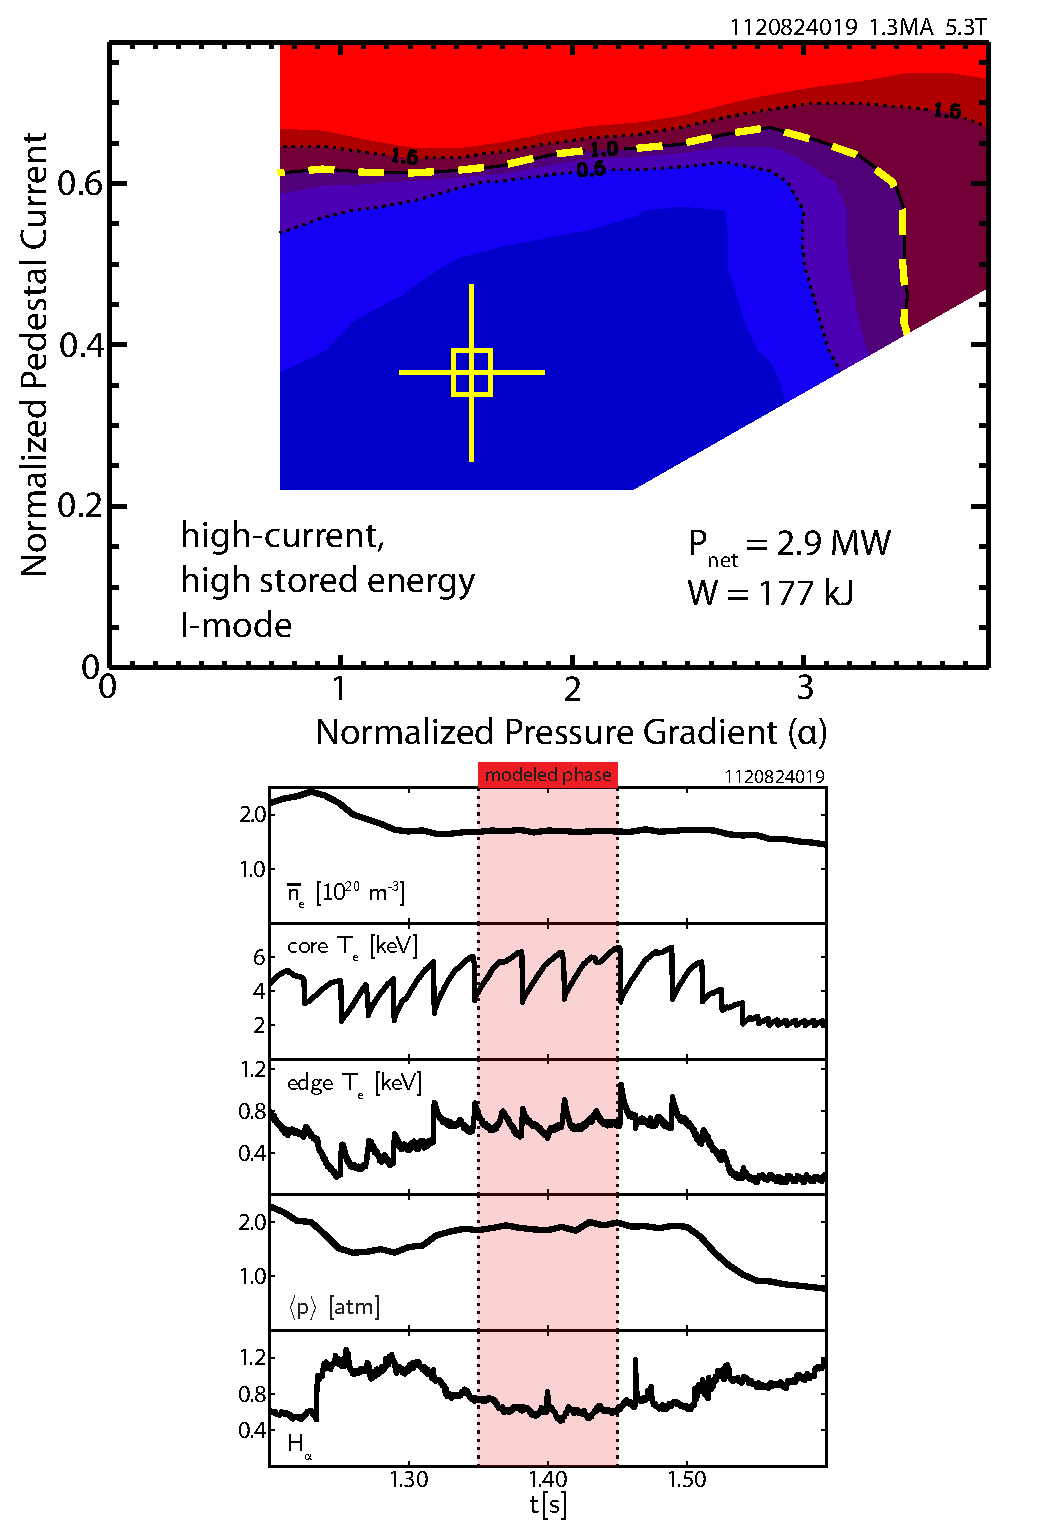
\includegraphics[width=150mm]{graphics/IModeModeling/1120824019_ELITE_stitch_vert.pdf}}{\caption[I-mode pedestal MHD stability contour generated by ELITE.]{MHD stability contour for a high-current ($\SI{1.3}{\mega\ampere}$), high-performance I-mode generated by the ELITE code.  The experimental measurement is shown by the crosshair, with the stability boundary indicated by the yellow dashed line.  Parameters for the modeled phase of the discharge are shown below.  The I-mode pedestal is observed to be far from both the peeling and ballooning MHD stability boundaries.}\label{fig:imode_elite_noelm}}
\end{figure}

Beginning from the experimental result, the profiles are scaled at fixed pedestal width, such that the pressure pedestal height or peak current density (with the current calculated by the Sauter formulation \cite{Sauter1999}) is increased or decreased relative to the original by a scalar factor, after which a self-consistent EFIT reconstruction is attempted.  This effectively fills in a grid in $\alpha_{MHD} - j$ space (a practice termed \emph{varyped}).  Horizontal slices represent a scaling of the pressure pedestal height (and therefore gradient) at fixed current, and vertical slices represent a scaling of the current density at fixed $\nabla p$.  While ELITE does not explicitly distinguish between density and temperature profiles, these slices implicitly vary density and temperature relative to each other.  For example, horizontal slices increase both density and temperature at roughly fixed $n_e/T_e^2$, such that collisionality is fixed, while vertical slices decrease pedestal density and increase temperature to preserve the pedestal pressure while decreasing collisionality, thereby increasing the bootstrap current (note that these trends are inexact, as the \emph{varyped} process attempts to generate self-consistent equilibria after scaling the pedestals in this fashion, which tends to skew the grid slightly).  Note that the practice described in \cref{sec:mod_eped} of increasing pressure (and pressure gradient) at fixed width to find the maximum ELM-stable pressure as a function of width is essentially a diagonal slice through the $\alpha_{MHD} - j$ grid: only the pressure profile is explicitly scaled, with the bootstrap current allowed to self-consistently vary, and will increase with increasing $\nabla p$.  At each point in the $\alpha_{MHD} - j$ grid, ELITE is run for a range of mode numbers (here $5 \le n \le 35$) to find the most unstable mode and its growth rate; this is normalized to diamagnetic stabilization effects by the threshold for instability onset, $\gamma_{MHD} > \omega_{*eff}/2$, where $\omega_{*eff}$ is the effective diamagnetic frequency accounting for variation in the pedestal, as implemented in EPED1.6 (see \cref{subsec:mod_eped16}).

\subsection{I-Mode ELITE Calculations}\label{subsec:imode_elite_calc}

An ELITE calculation for the I-mode pedestal is shown in \cref{fig:imode_elite_noelm}, along with parameters (line-averaged density, core and edge $T_e$, global-average pressure, and $H_\alpha$ emission) for the modeled phase of the discharge.  The I-mode pedestal parameters, indicated by the yellow crosshair, are far from both the peeling and ballooning MHD stability boundaries calculated by ELITE (indicated by the yellow dashed line, marking the $\gamma/(\omega_{*eff}/2) = 1$ contour) -- compare this with the ELMy H-mode calculation shown in \cref{fig:elmy_elite}.  This is consistent with the observed lack of large ELMs, even in higher-performance I-modes (both in the normalized sense, with $H_{98} = 1.02$ and $\beta_N = 1.0$, and in absolute terms, $W_{MHD} = \SI{177}{\kilo\joule}$ in the case in \cref{fig:imode_elite_noelm}, compared to $W \sim 100-\SI{120}{\kilo\joule}$ in ELMy H-mode and $W \sim 150-\SI{190}{\kilo\joule}$ in EDA H-mode).

\begin{figure}[h]
 \pushtooutside
 \fcapside[60mm]{\caption[Pedestal profiles in I-mode and ELMy H-mode.]{Pedestal profiles in I-mode and ELMy H-mode.  Due to the steep density gradient in the pedestal, the H-mode exhibits significant pressure gradient and edge current density, which drive the peeling-ballooning MHD instability associated with the ELM trigger.  Despite this, the high edge temperature in I-mode allows it to reach an appreciable pedestal pressure.}\label{fig:imode_elmy_profs}}{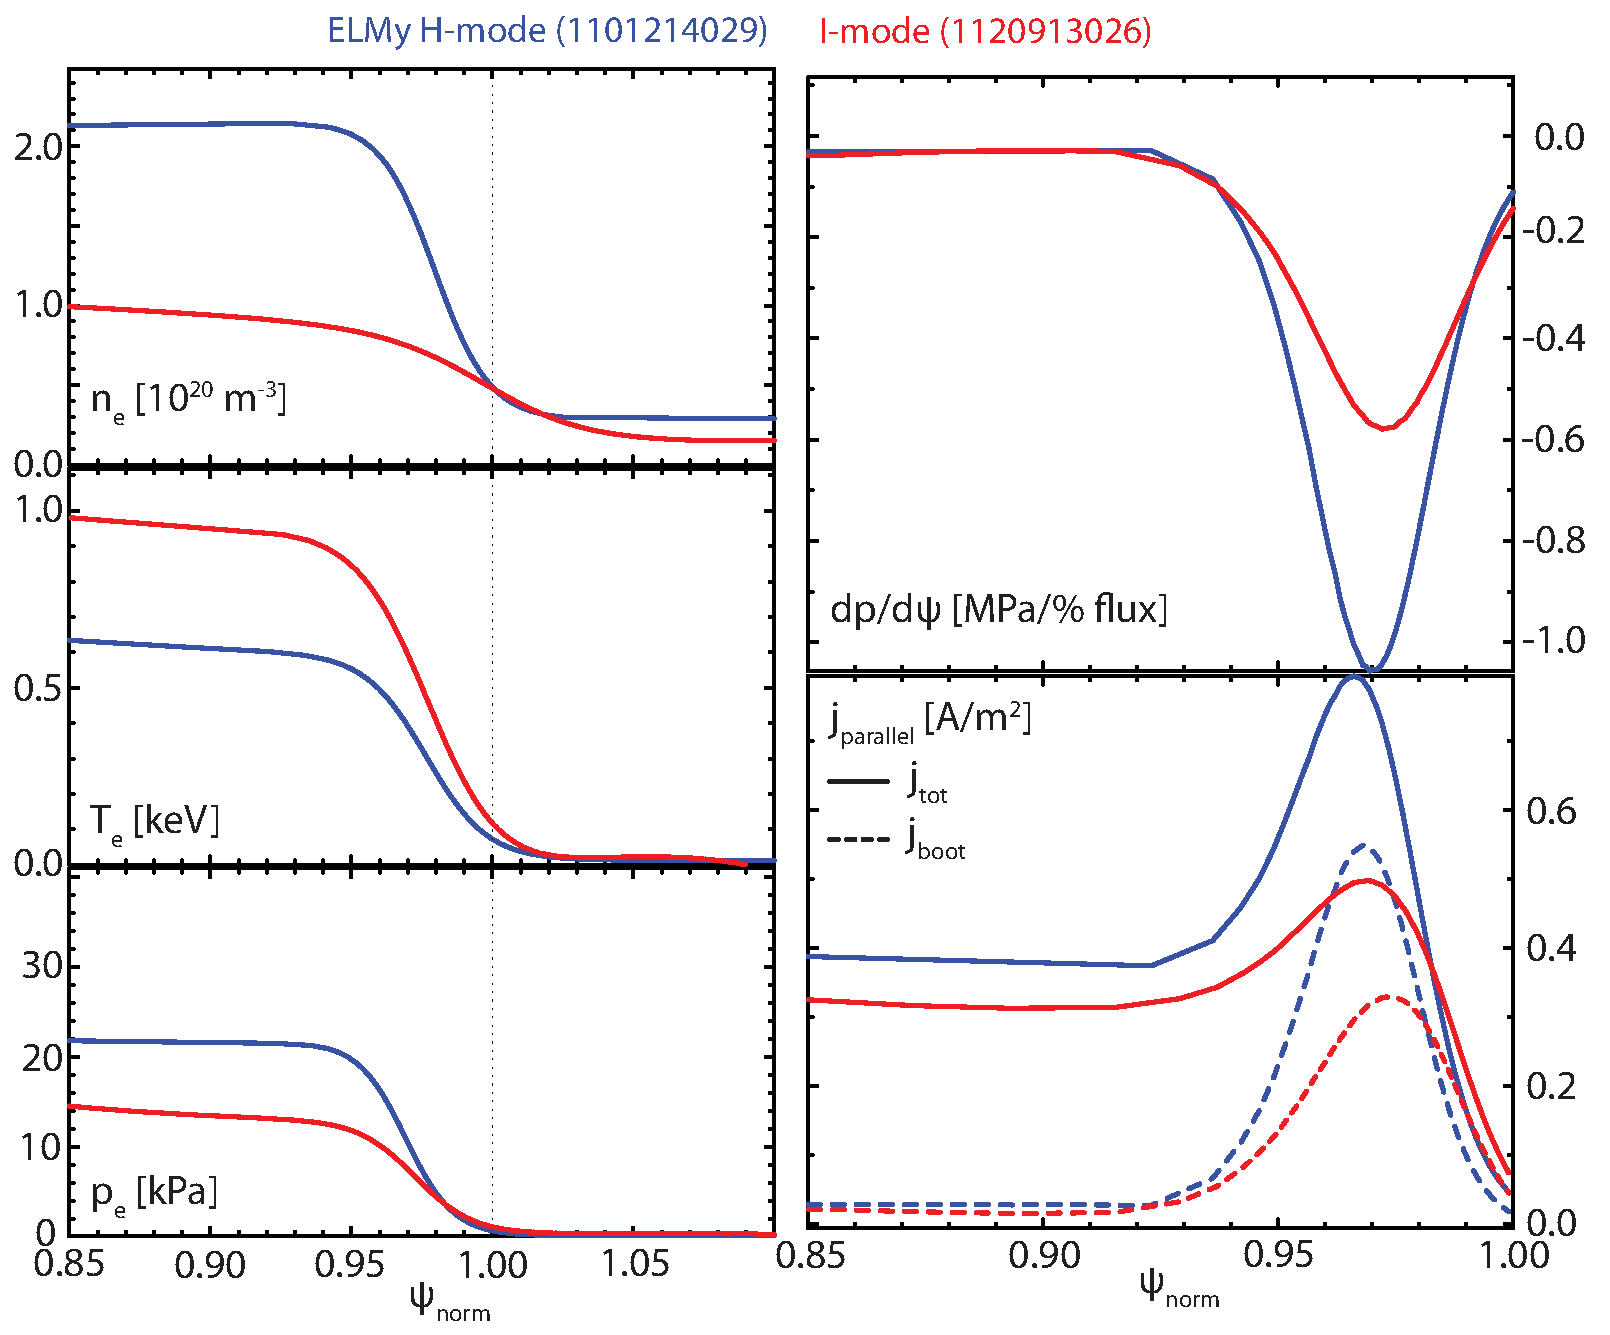
\includegraphics[width=100mm]{graphics/IModeModeling/prof_elmy_imode.pdf}}
\end{figure}

The calculated MHD stability is intuitively understood from the I-mode pedestal profile: while the I-mode reaches comparable pedestal pressures to H-mode, the pressure is due largely to the strong temperature pedestal, with a relaxed density profile and broader pedestal width than comparable-$\beta_p$ H-modes.  This reduces the total pressure gradient (and thus the ballooning MHD drive), as well as the local bootstrap current (set largely by the density gradient) and peeling drive.  A comparison of the pedestal profiles, with pressure gradient and edge current density, between I-mode and H-mode is shown in \cref{fig:imode_elmy_profs}.  However, due to the strong interplay between the pressure gradient and bootstrap current (which is reduced by the lack of a density pedestal, but enhanced by the naturally low collisionality in I-mode), the full computational approach in ELITE is necessary to accurately characterize the pedestal stability.

\begin{figure}[p]
 \pushtooutside
 \ffigbox[\FBwidth]{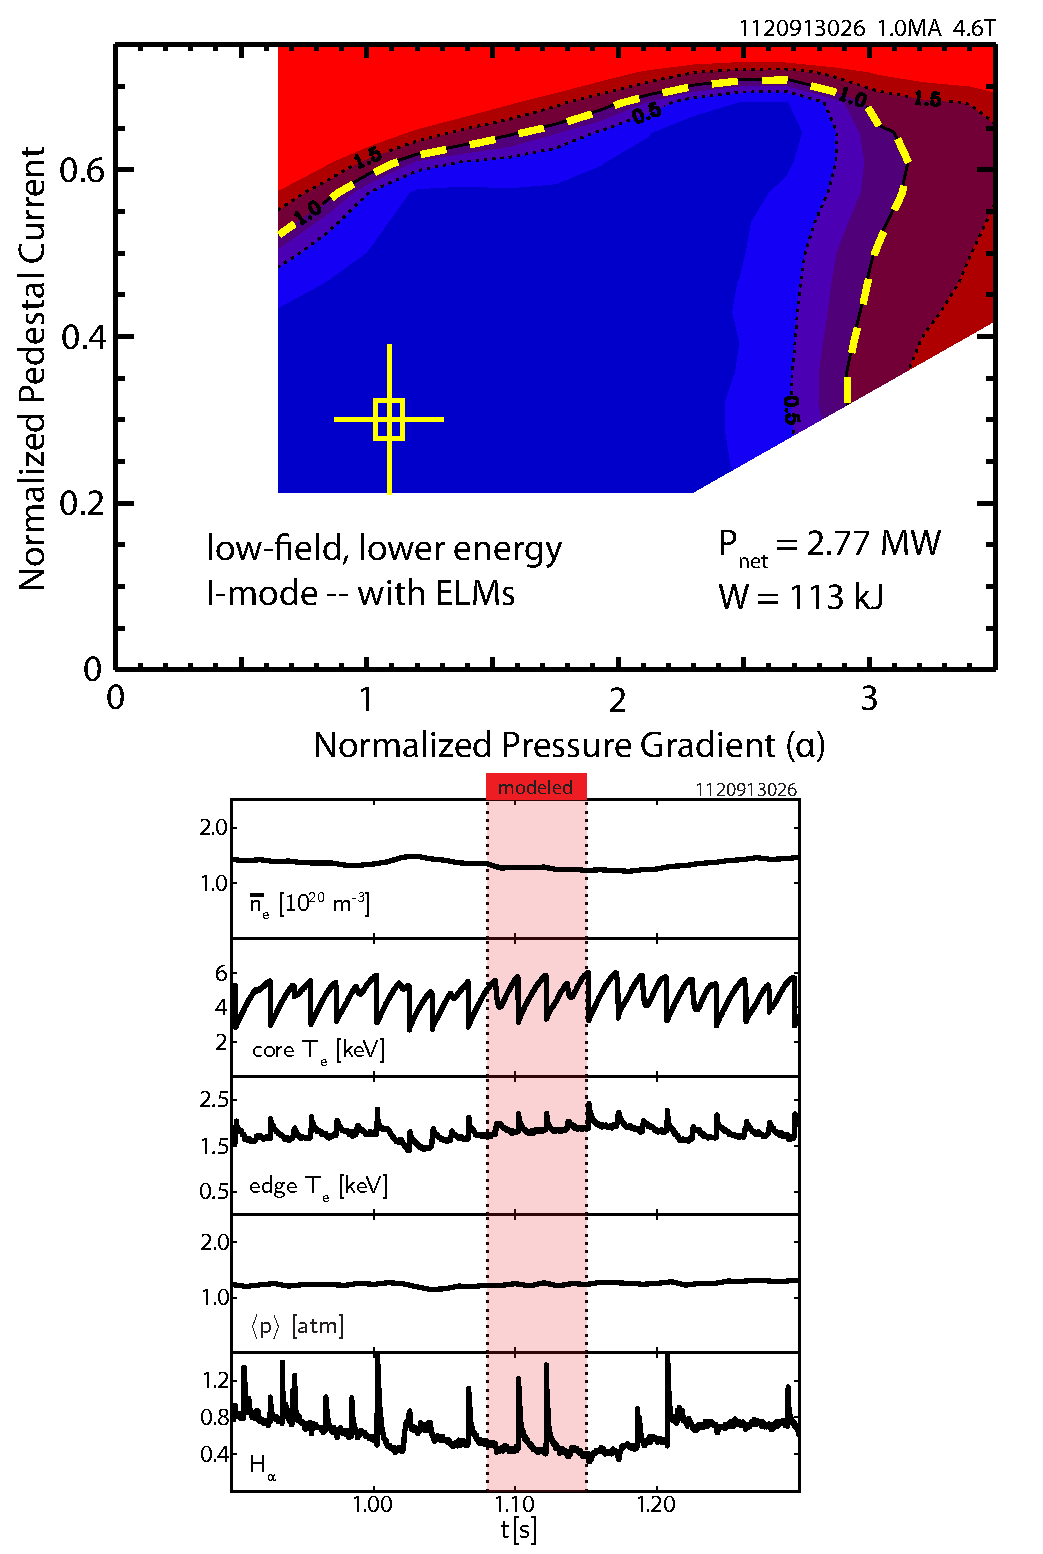
\includegraphics[width=150mm]{graphics/IModeModeling/1120913026_ELITE_stitch_vert.pdf}}{\caption[I-mode pedestal MHD stability contour generated by ELITE -- low-field case exhibiting ELM-like events.]{MHD stability contour for a low-field ($\SI{4.6}{\tesla}$), lower-energy I-mode generated by the ELITE code.  The experimental measurement is shown by the crosshair, with the stability boundary indicated by the yellow dashed line.  Parameters for the modeled phase of the discharge are shown below.  This case exhibited small,intermittent ELM-like events, but is still calculated to be peeling-ballooning stable for profiles averaged over the time window.}\label{fig:imode_elite_stelm}}
\end{figure}

Although I-mode is free of the regular, large ELMs typical of (type-I) ELMy H-mode, under certain conditions -- particularly reduced toroidal field and plasma current -- small ($<1\%$ drop in stored energy) intermittent ELM-like events are occasionally observed in I-mode.  However, when examined in ELITE (\cref{fig:imode_elite_stelm}) these cases are found to still be far from the peeling-ballooning boundary.  These intermittent events occur in conjunction to sawtooth heat pulses reaching the edge, visible on the fast ECE $T_e$ signal, indicating that the events are potentially triggered by transient modification of the pedestal by the heat pulse -- however, these events are not consistently triggered on each sawtooth crash under similar conditions.  More study is required on this front, with initial results shown in \cref{sec:imode_elms}.

\begin{figure}[p]
 \pushtooutside
 \ffigbox[\FBwidth]{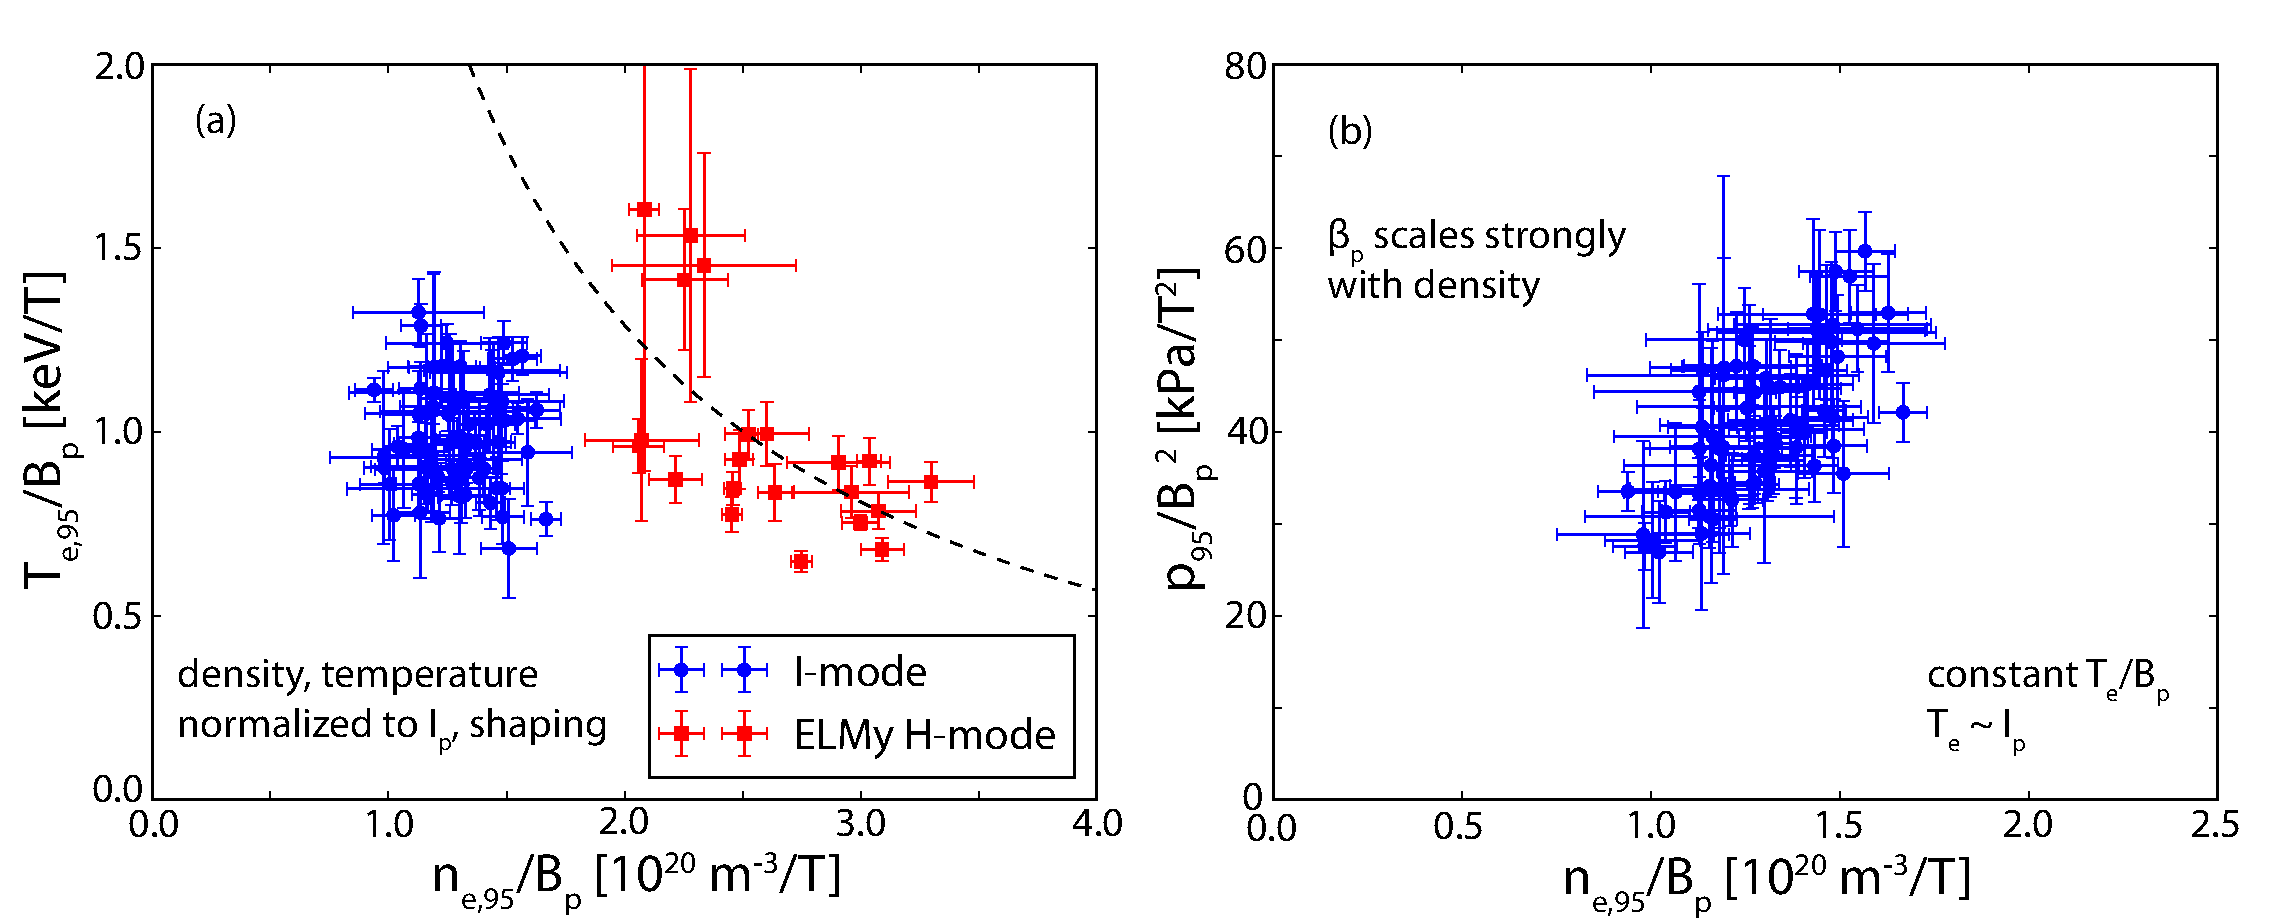
\includegraphics[width=150mm]{graphics/IModeModeling/neBp_stitch.pdf}}{\caption[Normalized pedestal temperature and pressure versus density.]{Pedestal temperature (left) and pressure (right) versus pedestal density.  Parameters are normalized to the edge poloidal field -- this accounts for plasma-current variation in the datapoints, as well as allowing a natural representation of MHD boundaries.  (a) Pedestal temperature vs. density for I-mode and ELMy H-mode.  Due to the poloidal-field normalization, hyperbolae in the parameter space are curves of constant $\beta_{p,ped}$.  ELMy H-modes lie, to lowest-order approximation, on a $\beta_{p,ped}$-limited curve (indicated by the dashed line) with the expected inverse relationship between density and temperature; I-mode $n_e$ and $T_e$, however, are uncorrelated.  (b) Pedestal pressure normalized to poloidal field pressure versus normalized density in I-mode.  Pedestal poloidal beta trends linearly with (normalized) density, rather than lying on the $\beta_{p,ped}$-limited line expected for MHD-limited pedestals, consistent with the strong response of the I-mode pedestal to fueling (see \cref{subsec:imode_fueling}).  I-mode data lie on a line of constant $T_e/B_p$, consistent with the observed $T_{e,ped} \sim I_p$ seen in \cref{subsec:imode_temp}.}\label{fig:neBp_stitch}}
\end{figure}

\begin{figure}[p]
 \pushtooutside
 \fcapside[60mm]{\caption[Normalized pedestal pressure vs. density, graded by power-per-particle.]{Pedestal pressure normalized to poloidal field pressure versus normalized density in I-mode (\cf \cref{fig:neBp_stitch}(b)).  Points are color-coded by power-per-particle, which sets the pedestal temperature -- differing values of $P_{net}/\overline{n}_e$ set the slope of the fixed $T_e/B_p$ line.  The increase in normalized pressure, then, is not solely due to increased power, but rather indicates a positive response with fueling.}\label{fig:neBp_pBp_Pnebar}}{\includegraphics[width=100mm]{graphics/IModeModeling/neBp_pBp_Pnebar.pdf}}
\end{figure}

Examination of the I-mode pedestal is also illuminating from the perspective of MHD stability.  To lowest order approximation, MHD-limited pedestals, as are found in ELMy H-mode, are limited in the attainable poloidal beta at the pedestal top (a limit arising from the limit on $\alpha_{MHD}$ from ballooning instability coupled with the weakly-varying pedestal width on a given tokamak -- \cf \cref{subsec:hcr_elmy_fluct}).  This is illustrated in \cref{fig:neBp_stitch}(a), showing the pedestal density and temperature normalized to poloidal field (accounting for variation in plasma current).  Due to the normalization to $B_p$, hyperbolae in the parameter space are curves of constant pedestal $\beta_{p}$.  ELMy H-mode data lie on such a curve (note that, since the $\beta_p$ limit is shaping-dependent, only ELMy H-mode cases with approximately matched shape are shown on the single hyperbolic curve), with the expected inverse relationship between pedestal density and temperature.  I-mode pedestal density and temperature, on the other hand, are uncorrelated, consistent with the pedestal not being limited by MHD stability constraints.  I-mode pedestal pressure, similarly normalized, is shown against normalized pedestal density in \cref{fig:neBp_stitch}(b).  Where MHD-limited pedestals would show a flat trend due to the limit on poloidal beta, I-mode $\beta_p$ instead exhibits a linear trend with density.  This is consistent with the strong response of pedestal performance with increased fueling (described in \cref{ch:ImodePedestal}, particularly \cref{subsec:imode_fueling}) provided sufficient heating power to maintain the pedestal.  The slope of this trend is a line of constant $T_{e,95}/B_p$, consistent with the observed $T_e \sim I_p$ as well (see \cref{subsec:imode_temp}).  This trend in the normalized pressure is in addition to the response of pedestal pressure with heating power, as shown in \cref{fig:neBp_pBp_Pnebar}.  The temperature response to heating power is encoded in setting the slope of the fixed $T_{e,95}/B_p$ line, reflecting the higher temperatures at fixed current with increased $P_{net}/\overline{n}_e$.\nicesectionending

\section{Kinetic-Ballooning Mode Stability}\label{sec:imode_baloo}

\begin{figure}[t]
 \pushtooutside
 \ffigbox[\FBwidth]{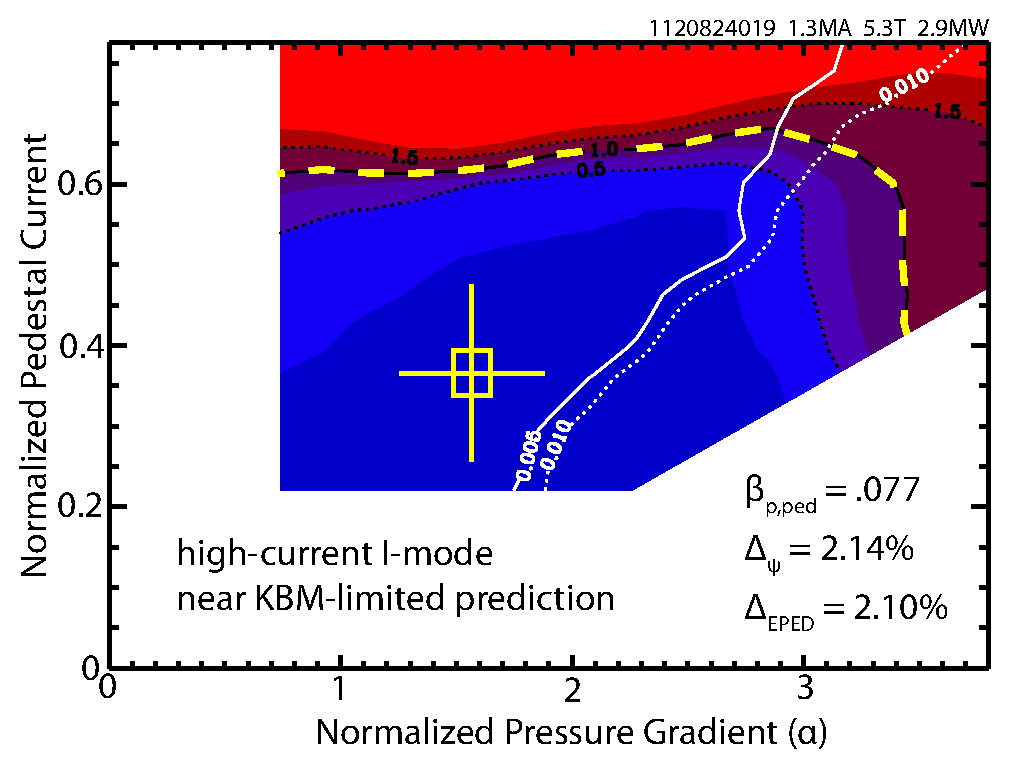
\includegraphics[width=150mm]{graphics/IModeModeling/1120824019_1400n5_35_gamws16_bal.pdf}}{\caption[Infinite-$n$ ballooning MHD prediction, overlaid on ELITE result (\cref{fig:imode_elite_noelm}).]{Infinite-$n$ ballooning MHD results calculated by BALOO, overlaid on the ELITE results for the same case (see \cref{fig:imode_elite_noelm}).  The Infinite-$n$ ballooning threshold is taken as a surrogate for the onset of KBM turbulence.  Due to the local nature of the infinite-$n$ constraint, BALOO calculates the width in flux space that is locally ballooning-critical -- when this reaches half of the pedestal width, the KBM is assumed to be triggered.  This case is near the KBM-predicted pedestal width $\Delta_{EPED}$, but is nevertheless modeled to be KBM-stable (for $\Delta_\psi \sim 0.02$, the half-width threshold is the white dotted contour labeled $0.01$).}\label{fig:imode_baloo_noelm}}
\end{figure}

\begin{figure}[t]
 \pushtooutside
 \ffigbox[\FBwidth]{\includegraphics[width=150mm]{graphics/IModeModeling/1120913026_1186n5_35_bal_jalpha.pdf}}{\caption[Infinite-$n$ ballooning MHD prediction, overlaid on ELITE result (\cref{fig:imode_elite_stelm},-- pedestal profiles for this case are also shown in \cref{fig:imode_elmy_profs}).]{Infinite-$n$ ballooning MHD results calculated by BALOO, overlaid on the ELITE results for the same case (see \cref{fig:imode_elite_stelm}).  This case exhibited sawtooth-triggered ELM-like events.  This case is substantially wider than the KBM-predicted pedestal width $\Delta_{EPED}$, and is modeled to be strongly KBM-stable -- in fact, the BALOO assay could not calculate enough ballooning-unstable rational surfaces to draw the contour for the BCP-predicted threshold of $0.02$.}\label{fig:imode_baloo_stelm}}
\end{figure}

Edge turbulence in I-mode is characterized by the strong reduction of mid-frequency turbulence corresponding to the reduced energy transport after the L-I transition.  Instead, the I-mode exhibits a broad higher-frequency ($200-400\;\si{\kilo\hertz}$) fluctuation, the \emph{Weakly-Coherent Mode} \cite{Whyte2010,Hubbard2011,Cziegler2013} (see \cref{subsec:hcr_imode_wcm}).  Due to its prominence in the I-mode edge and qualitative similarity to the Quasi-Coherent Mode (QCM) in EDA H-mode \cite{Hubbard2001} (see \cref{subsec:hcr_eda}), the WCM is thought to play a role in regulating the I-mode pedestal, particularly by driving enhanced particle flux \cite{Dominguez2012}.  While the WCM is fairly well-characterized experimentally, the underlying physics of the mode remain an open question.  From the standpoint of both turbulence characterization and ELM stability, the kinetic-ballooning mode (KBM) is a valuable starting point for comparing the WCM to the turbulent behavior in more conventional H-modes.

Computational modeling of the KBM is possible using infinite-$n$ ideal ballooning MHD as a surrogate for the turbulence threshold \cite{Snyder2001,Candy2005,Snyder2009} (see \cref{sec:mod_turbulence}).  The localized constraint from the KBM (and perfectly-localized infinite-$n$ ideal MHD) is applied to the entire pedestal via the ``ballooning-critical pedestal'' technique, described in \cref{subsec:mod_bcp}, in which the KBM threshold is identified as the point at which half of the pedestal (typically the ``middle half'' where the pressure gradient is steepest) is locally at or beyond criticality to the MHD surrogate.  This is calculated using the BALOO code \cite{Connor1979,Miller1987}; at each point in the \emph{varyped} grid, the number of rational surfaces that are unstable to infinite-$n$ ballooning modes and subsequently the width in poloidal flux space covered by these surfaces is calculated, drawing contours of pedestal half-width corresponding to the KBM threshold.

I-mode pedestals exhibit little trend in width (in poloidal flux space) with pedestal poloidal beta (see \cref{fig:imode_wid_betapol}), as would be expected for pedestals limited by KBM turbulence.  We may compare cases spanning the range in pedestal width $\Delta_\psi$ against the KBM-limited prediction for the width, $\Delta_\psi = 0.076 \beta_{p,ped}^{1/2}$, from EPED1 (see \cref{subsec:mod_eped1}), herein termed $\Delta_{EPED}$.  A representative case near the EPED1 prediction line is shown in \cref{fig:imode_baloo_noelm} (overlaid on the ELITE result for the same case, \cref{fig:imode_elite_noelm}).  For $\Delta_\psi = .021$, the expected KBM threshold based on the BCP half-width calculation is the $0.01$ contour -- the pedestal is calculated to be stable compared to this threshold.  The representative case far from the EPED1 prediction line is shown in \cref{fig:imode_baloo_stelm} (overlaid on the ELITE result for the same case, \cref{fig:imode_elite_stelm}).  At $\Delta_\psi = 0.04$, the expected KBM threshold is the $0.02$ contour -- however, the BALOO assay could not calculate enough ballooning-unstable rational surfaces to even draw this contour.  Suffice to say that the pedestal is far from the KBM onset threshold as calculated from infinite-$n$ MHD.  Notably, the former case ($\Delta_\psi \sim \Delta_{EPED}$) was a relatively high-performance case, and did not exhibit ELM-like events, while the latter ($\Delta_\psi \gg \Delta_{EPED}$) exhibited ELM-like events.  The indication from both experimental observation (namely, the lack of dependence of the pedestal width on $\beta_{p,ped}$) and computational modeling, then, is that the KBM is not responsible for limiting the pedestal in I-mode.\nicesectionending

\section{Intermittent ELMs in I-Mode}\label{sec:imode_elms}

Given the importance of controlling or avoiding large ELMs on ITER- and reactor-scale devices, a firm understanding of the physics underlying the ELM trigger is essential for planned ITER operation.  While I-mode is typically observed to be naturally free of large, damaging ELMs, there are nevertheless a minority of cases -- twelve time windows comprised of ten unique shots, out of 72 windows (52 unique shots) total in the pedestal database -- under certain conditions (particularly, reduced current and toroidal field) in which small, intermittent ELMs or ELM-like events are observed.  It is to these cases that we now turn our attention.

\begin{figure}[p]
 \pushtooutside
 \ffigbox[\FBwidth]{\includegraphics[width=150mm]{graphics/IModeModeling/1120830028_prof_stbin.pdf}}{\caption[Density and temperature profiles in I-mode, showing the modification of the temperature pedestal by the sawtooth heat pulse.]{Profiles of $n_e$ and $T_e$ in the I-mode pedestal, with the full ensemble-averaged data (black) compared to data masked to the first 25\% of the sawtooth cycle following the heat pulse reaching the edge.  The sawtooth does not meaningfully perturb the density profile, but triggers a measurable transient increase in the temperature pedestal.}\label{fig:prof_stbin}}
\end{figure}

\begin{figure}[p]
 \pushtooutside
 \ffigbox[\FBwidth]{\includegraphics[width=150mm]{graphics/IModeModeling/1120830028_stbin_elite.pdf}}{\caption[Peeling-ballooning MHD and KBM stability in I-mode, showing modification by sawtooth heat pulse.]{Peeling-ballooning MHD stability calculated by ELITE and KBM thresholds calculated by BALOO for an I-mode case, comparing the time-averaged data against pedestal profiles prepared with data masking to the first 25\% of the sawtooth cycle following the heat pulse reaching the edge (see \cref{fig:prof_stbin}).  Note that, to directly compare two separately-calculated equilibria, we replace the $\alpha_{MHD}$ and $j_\parallel$ axes with stability metrics arising from peeling and ballooning MHD.  While the sawtooth heat pulse does measureably perturb the pedestal in stability space, it is insufficient to reach either the peeling-ballooning or KBM threshold.}\label{fig:imode_stbin}}
\end{figure}

ELMs in I-mode are generally observed to be small ($<1\%$ perturbation to the stored energy), and are sporadic, rather than occurring in a regular cycle as in the conventional type-I ELMy H-mode.  The majority events occur shortly following the sawtooth heat pulse reaching the edge (26 sawtooth-triggered events in the studied windows, compared to 10 off of the sawtooth), based on timing from fast ECE $T_e$ measurements in the pedestal.  This indicates a possible trigger for the event due to transient modification of the pedestal structure.  An example case of this is shown in \cref{fig:prof_stbin}.  The sawtooth heat pulse does not perturb the density profile, but drives a significant transient increase in the temperature pedestal (data masked to the first 25\% of the sawtooth cycle after the heat pulse reaches the edge shown in red).  Calculations in ELITE and BALOO for this case are shown in \cref{fig:imode_stbin} for both the time-averaged pedestal profile, and the masked data to the sawtooth cycle.  While the sawtooth synchronization does drive a measurable perturbation to the pedestal in stability space -- the effect is predominantly in the pressure gradient, rather than the current density, due to the weaker effect of the temperature gradient on the bootstrap current -- the effect is insufficient to reach either the peeling-ballooning MHD or the KBM turbulence threshold (although the perturbed point nears the KBM threshold within errorbars, indicating that the KBM may still be a factor).  Note that, in order to compare two separately-computed equilibria, we use alternate axes in \cref{fig:imode_stbin}: rather than directly using $\alpha_{MHD}$ and the (normalized) edge current density, the parameter space is presented in terms of ballooning and kink-peeling stability parameters, $\beta_N/\Delta^{3/4}$ and $j_{max} \Delta^{1/4}$.  The first encapsulates the $p_{ped} \sim \Delta^{3/4}$ trend expected from ballooning stability, when accounting for the nonlocal effects -- at broader $\Delta$, wider low-$n$ modes destabilize more easily, reducing the maximum $\alpha_{MHD}$, as described in \cref{sec:mod_pb} -- and current stabilization.  The second accounts for the trend in the total current, $\int j \;d\psi \sim \Delta^{3/4}$ from the $p_{ped} \sim \Delta^{3/4}$ trend from ballooning stability, with the total edge bootstrap current set by the pedestal pressure; however, the maximum current density and total pedestal current may be related by $\int j \; d\psi \sim j_{max} \Delta \rightarrow j_{max} \sim 1/\Delta^{1/4}$, thus the current-driven kink/peeling stability may be expressed in terms of the normalized $j_{max} \Delta^{1/4}$.

\begin{figure}[!b]
 \pushtooutside
 \ffigbox[\FBwidth]{\includegraphics[width=150mm]{graphics/IModeModeling/trace_elmy_imode_2.pdf}}{\caption[ELM traces for H-mode and I-mode.]{Traces of $n_{l04}$, core and edge ($r/a \sim 0.98$) $T_e$, and $H_\alpha$ for ELMy H-mode (left) and I-mode (right).  ELMs in H-mode (visible on the $H_\alpha$ trace) are independent of the sawtooth cycle, and drive perturbations to the edge temperature and line-integrated density, as both energy and particles are expelled form the plasma by the ELM crash.  This is particularly clear on the edge temperature, which exhibits a clear increase with the sawtooth heat pulse and a separate crash with the ELM.  I-mode, in contrast, exhibits ELMs (or ELM-like events) that are tied to sawtooth heat pulses reaching the edge, as visible on the ECE $T_e$ signal.  No visible crash in edge temperature is visible following the ELM, nor is there a significant perturbation to the density.}\label{fig:trace_elmy_imode}}
\end{figure}

In light of the observed stability of I-mode to peeling-ballooning MHD -- even in cases where the perturbation of the putative sawtooth trigger is accounted for -- it is worthwhile to examine the behavior of the ELMs in I-mode compared to those found in more conventional H-modes.  Traces from a type-I ELMy H-mode and an I-mode are shown in \cref{fig:trace_elmy_imode}.  The ELMy case (left) exhibits behavior typical of a type-I ELM cycle: discrete, regular ELMs (visible on the $H_\alpha$ trace), with crashes in edge temperature as the ELM expels energy and particles into the SOL.  The effects of the sawteeth are distinct from the ELM, with a spike and subsequent relaxation in edge temperature from the heat pulse visible on the edge ECE $T_e$ separate from the sharp temperature-pedestal crash due to the ELM.  The sporadic sawtooth-triggered events in I-mode (right), despite a similar trace in $H_\alpha$, do not exhibit the characteristic crash in edge temperature associated with an ELM -- rather, only the spike in $T_e$ from the sawtooth heat pulse is visible, followed by a relaxation to the steady pedestal temperature.

The distinction between the two edge perturbations is visible in a single case, shown in \cref{fig:trace_imode_welms}.  The sawtooth heat pulse at $\SI{0.87}{\second}$ triggers an I-H transition, indicated by the reduction in $H_\alpha$ light following the pulse from the sawtooth, and the sudden reduction in turbulence visible in the $\tilde{n}_e$ spectrogram (both destroying the WCM fluctuation at $\sim \SI{300}{\kilo\hertz}$, and further reducing the mid-frequency broadband turbulence).  Such a transition is not unheard-of -- recall that the L-I transition is tied to sawtooth heat pulses as well.  This H-mode terminates with a non-sawtooth-triggered ELM at $\SI{0.885}{\second}$, with the customary crash in edge temperature and $H_\alpha$ spike.  After the H-mode terminates, the plasma reverts to I-mode, with a further sawtooth-triggered event at $\SI{0.91}{\second}$.  Although there does appear to be some $T_e$ reduction due to the ELM, it is insufficient to outweigh the $T_e$ spike from the sawtooth heat pulse.

\begin{figure}[t]
 \pushtooutside
 \fcapside[60mm]{\caption[I-mode with a brief H-mode terminated by an ELM, as well as sawtooth-triggered ELM-like events.]{Traces of $n_{l04}$, core and edge $T_e$, and $H_\alpha$ for an I-mode exhibiting ELM-like events.  The sawtooth heat pulse at $\sim \SI{0.87}{\second}$ triggers an I-H transition, indicated by the drop in $H_\alpha$ and suppression of turbulence visible on the $\tilde{n}_e$ plot.  This H-mode terminates with a non-sawtooth-triggered ELM with visible edge temperature crash and density perturbation, dropping back into I-mode.  The I-mode phase also exhibits sawtooth-triggered ELM-like events with minimal density perturbation or temperature crash.}\label{fig:trace_imode_welms}}{\includegraphics[width=100mm]{graphics/IModeModeling/trace_imode_welms_2.pdf}}
\end{figure}

Given that these majority cases (shown in \cref{fig:trace_elmy_imode} at right) do not exhibit the expected temperature pedestal crash and are MHD-stable, it is apparent that these cases are not instability-triggered ELMs at all, but rather are a distinct, and far more benign, phenomenon.  For clarity, we will call these ``sawtooth $H_\alpha$ spikes'' (indeed, this seems to be the only distinguishing factor for these edge events!).  A plausible explanation is that the sawtooth does not trigger an instability in the edge, but instead propagates into the scrape-off layer.  The heat pulse then creates a propagating ionization front as it encounters the cold plasma and neutral gas in the SOL.  The burst of $H_\alpha$ light and subsequent exponential decay is due to this sudden pulse energizing neutrals in the edge.  Fundamentally, the $H_\alpha$ spike from a conventional ELM is driven by the same cause -- a sudden influx of particles and energy into the SOL, as well as a similar ionization front in the neutrals in the far SOL.  However, the underlying phenomenon of these events is not entirely clear -- even under comparable conditions, the spikes are not consistently triggered by similarly-sized sawtooth heat pulses.  The edge behavior of these cases is therefore a subject of continuing investigation.

\begin{figure}[p]
 \pushtooutside
 \ffigbox[\FBwidth]{\includegraphics[width=150mm]{graphics/IModeModeling/1120907010_ELITE_stitch_vert_v2.pdf}}{\caption[I-mode pedestal stability contour generated by ELITE and BALOO -- case exhibiting a non-sawtooth-triggered ELM]{MHD stability contour for I-mode generated by the ELITE code, with results from the infinite-$n$ BALOO calculation overlaid.  The experimental measurement is shown by the crosshair, with the stability boundary indicated by the yellow dashed line.  Parameters for the modeled phase of the discharge are shown below.  This case exhibited a solitary ELM not triggered by the sawtooth heat pulse, with the characteristic edge temperature crash of a canonical ELM.  However, the I-mode phase around the ELM is calculated to be peeling-ballooning stable and below the KBM threshold.}\label{fig:imode_elite_nonstelms}}
\end{figure}

In addition to the sawtooth-triggered $H_\alpha$ spike events described above, a minority of edge $H_\alpha$ events do exhibit the characteristic temperature crash of an ELM, and are not in all cases triggered by a sawtooth (although some of these cases may be compound ELMs following a sawtooth-triggered event).  Peeling-ballooning and KBM stability analysis of such a case is presented in \cref{fig:imode_elite_nonstelms}.  In this case, a single ELM is visible at $\SI{1.1}{\second}$, independent of the sawtooth cycle -- rather, the characteristic crash is visible in the edge temperature after relaxation of the temperature from the sawtooth heat pulse (note, however, that the ELM does not significantly perturb the stored energy/global-averaged pressure).  When modeled in ELITE and BALOO, however, the steady I-mode phase around the ELM is nevertheless found to be well into the stable region both for infinite-$n$ ballooning modes and finite-$n$ coupled peeling-ballooning modes.  While it is possible that a transient effect not captured by the profiles used for the stability calculation drove the pedestal near the classical ELM stability boundary in this case, the stationary state for the plasma is evidently stable to the expected ELM triggers.\nicesectionending

\section{Summary \& Discussion}\label{sec:imode_mod_conclusions}

Models for the trigger of large, deleterious ELMs based on coupled peeling-ballooning MHD instabilities \cite{Wilson2002,Snyder2003,Snyder2004,Wilson2006} and kinetic-ballooning turbulence \cite{Snyder1999,Candy2005,Snyder2001} have been particularly successful in capturing the physics underlying the ELMy H-mode pedestal.  This approach is applied to the I-mode pedestal.  The majority of I-mode cases are naturally free of ELMs, and are modeled to be strongly stable both to coupled peeling-ballooning MHD modes and to KBM turbulence (calculated by way of the infinite-$n$ ideal-ballooning MHD surrogate).  Under certain conditions, particularly reduced plasma current and magnetic field, the I-mode exhibits small, intermittent ELM-like events.  The majority of these cases are evidently tied to the sawtooth heat pulse reaching the plasma edge, and lack the characteristic edge temperature crash expected due to the expulsion of energy and particles by the ELM.  This, coupled with the computed stability of these pedestals (even when the data are treated to account for the transient modification of the temperature pedestal by the sawtooth), suggests that the phenomenon is distinct from a traditional type-I ELM, with the measured spike in $H_\alpha$ light (customarily indicative of an ELM) possibly driven by an ionization front in the SOL from the sawtooth heat pulse propagation, rather than an explosive edge instability.  A minority of ELM events in I-mode exhibit the characteristic $T_e$ crash, including some events that are not evidently triggered by the sawtooth heat pulse.  The steady I-mode phases around these events, however, are also modeled to be stable, indicating a transient event not captured by these models driving the ELM instability.

This assay into the computed stability of I-mode is consistent with the observed absence of large, deleterious type-I ELMs in I-mode.  This stability is self-enforcing, from the fundamental nature of the I-mode pedestal -- the pressure pedestal is set largely by the strong temperature pedestal, with the flat density profile suppressing both the pressure gradient and the bootstrap current drive.  For minority of I-mode cases exhibiting apparent ELMs, most cases are evidently not ``true'' instability-driven ELMs, but are rather a benign sawtooth-triggered $H_\alpha$ spike.  In the minority of edge events, an edge temperature crash is present, indicating an ELM; however, these crashes are small ($<1\%$ perturbation to stored energy), with the temperature crash in sawtooth-triggered cases insufficient to overcome the positive effect of the heat pulse on the edge temperature.  Moreover, these I-mode cases exhibiting ELMs are typically the \emph{lower} performance cases, with less agressive fueling and heating power, reaching lower pedestal beta.

It is worth noting that more conventional ``ELM-suppressed'' regimes (\eg RMP-suppressed H-modes, QH-mode) also can still present ELMs, with the suppression resulting in smaller, less dangerous ELMs rather than completely removing them.  While some ELM behavior is evidently endemic to high-performance pedestals, this behavior is limited in I-mode to small, intermittent events -- the existing I-mode parameter space is naturally stable against large (type-I) ELMs, as desired for a putative reactor regime.\nicechapterending

\bibliographystyle{../plainurl}
\bibliography{../references}
\chapter{Conclusions \& Future Work}\label{ch:Conclusion}

The work described in this thesis has contributed to the study of the pedestal in high-performance regimes -- as the pedestal sets a strict constraint on the core pressure and fusion power density, as well as deterimining the stability against large, deleterious Edge-Localized Modes (ELMs), a firm understanding of the physics entailed in the structure and stability of the pedestal is essential to the development of operating scenarios for ITER- and reactor-scale devices.  To this end, this thesis details a combined approach using both empirical observations and theoretical/computational models to understand the governing physics of the pedestal.\gnote{opener section should be work predating thesis -- be sure this is clear}

These analysis methods are developed first for ELMy H-mode experiments on Alcator C-Mod -- as this is the most broadly-accessible and well-understood high-performance regime on most tokamak devices (see \cref{ch:HighPerformance}), ELMy H-mode is considered the baseline for high-confinement operation on ITER \cite{Shimada2007}.  However, large, uncontrolled ELMs can drive pulsed heat loading and erosion damage in excess of the material tolerances of plasma-facing components.  Understanding the limits placed on the pedestal by ELM stability, then, is of critical importance for planned operation on ITER.  The work presented in this thesis (see also \cite{Walk2012}) was undertaken as a contribution to a joint research effort across several machines \cite{Groebner2013} to develop a predictive model for the ELMy H-mode pedestal.  

The empirical and computational analyses developed for ELMy H-mode are also applied in this thesis to the I-mode \cite{Whyte2010}, a novel high-confinement regime developed on Alcator C-Mod, with a number of highly desirable characteristics for reactor operation.  I-mode is notable in that it decouples energy and particle transport, forming an H-mode-like temperature pedestal with high energy confinement while maintaining an L-mode-like density profile with low particle confinement and favorably rapid transport of impurities from the plasma.  Moreover, the energy confinement in I-mode appears to degrade significantly more weakly than H-mode.  The work in this thesis (see also \cite{Walk2014}) focuses on characterizing the I-mode pedestal in terms of its structure and impact on global performance -- and therefore implications for operation on larger devices -- and its inherent avoidance of the instabilities associated with the ELM trigger.\nicesectionending

\section{Contributions to ELMy H-Mode Physics}\label{sec:conc_elmy}

ELMy H-mode experiments on C-Mod, described in \cref{ch:Elmy}, significantly expand the parameter range of investigation: C-Mod operation reaches the highest thermal pressure of any tokamak, up to within a factor of $\sim 2$ of the target pedestal pressure for ITER, as well as reaching the highest magnetic field at $\SI{8}{\tesla}$.  These experiments also entailed a significant scan in plasma current ($400-\SI{1100}{\kilo\ampere}$) and field ($3.5-\SI{8}{\tesla}$), representing a broad parameter range well outside of the explored operational space on other devices, at ITER-like conditions in several respects (\eg field, density, pressure).

%The pedestal in ELMy H-mode\gnote{move this up a section, or shorten to reference?} is thought to be limited by two key physics aspects: first, that the rapid onset of peeling-ballooning MHD instabilities (described in \cref{sec:mod_pb}) driven by the steep pressure gradients and high bootstrap current densities in the pedestal drives the explosive burst of ELM transport in the edge, and second, that the strong transport driven by kinetic-ballooning mode (KBM) turbulence, described in \cref{sec:mod_turbulence}, above an onset threshold limits the pedestal (particularly the pressure gradient) leading up to the ELM.  

The observed behavior in the pedestal are consistent with limits based in peeling-ballooning MHD instability and kinetic-ballooning turbulence (described in \cref{sec:mod_pb} and \cref{sec:mod_turbulence}, respectively).  Over the scan in plasma current (see \cref{sec:elmy_engineer}), the pressure pedestal height exhibits a trend of $p_{ped} \sim I_p$, while the pressure pedestal width scales as $\Delta_{p_e} \sim I_p^{-1}$.  Within this trend, the density and temperature pedestal widths individually exhibit no systematic trend with the plasma current, while the density and temperature pedestal heights both exhibit a weakly-positive trend with current.  This behavior is consistent with the expected $\nabla p \sim I_p^2$ constraint expected from the ballooning MHD stability limit; however, there is significant scatter, which may be corrected with a more refined analysis accounting for the pedestal width.  The attainable poloidal beta at the pedestal top is set largely by plasma shaping -- this is consistent with the ballooning MHD limit, constrained in terms of $\alpha_{MHD} \sim d\beta_{p}/d\psi$, which over the fairly restricted pedestal width sets (to zero'th order approximation) a limit on $\beta_{p,ped}$, with the attainable beta increasing with shaping due its stabilizing effect on the MHD mode.

The pedestal width is seen to scale as $\Delta \sim \beta_{p,ped}^{1/2}$, as expected from KBM turbulence (\cf \cref{subsec:elmy_eped_width}, particularly \cref{fig:elmy_betap_deltapsi_betabin}).  Alternate width models (\cref{subsec:elmy_width_oldmodels}) are largely discounted -- the density pedestal width does not exhibit the inverse dependence on the pedestal density expected from neutral-penetration models, while the temperature pedestal exhibits no dependence on the poloidal gyroradius, in contrast to predictions based on ion-orbit loss influence on the $\vec{E}\times\vec{B}$ sheared flow.  The pressure pedestal width variation with poloidal gyroradius is explained by the strong co-variance between $\rho_{i,pol}$ and $\beta_{p,ped}$.  The scatter in the pedestal height versus plasma current is corrected by accounting for this variation in width.  Taking the pedestal height to scale as $p_{ped} \sim \nabla p \times \Delta_p$, the pedestal height is predicted well by the combination of the ballooning MHD limit and the width scaling above, $p_{ped} \sim I_p^2 \beta_{p,ped}^{1/2} \sim I_p \sqrt{n_{e,ped} T_{e,ped}}$.

Strictly, the KBM model allows for secondary variation on shaping and collisionality on the mode threshold, taking the form $\Delta = G(\nu^*,\varepsilon,...) \beta_{p,ped}^{1/2}$ where $G$ is a weakly-varying function (taken to be constant in the simplest model).  The scale function is fitted to an average value $\langle G \rangle = 0.0857$, with no systematic depedence of the width on field, collisionality, shaping, or toroidal gyroradius observed (\cref{subsec:elmy_normwidth}).  

ELMy H-mode pedestals are also tested against results from the EPED model \cite{Snyder2011}, described in \cref{sec:mod_eped}, which operates based on self-consistent calculations of the peeling-ballooning MHD and KBM turbulence limits.  Notably, EPED bases its calculations only on engineering target parameters, such that it may be used predictively, rather than relying on reconstructed experimental data.  EPED predictions (see \cref{sec:elmy_eped}) for the pressure pedestal width and height match the observed results to within the $\sim 20\%$ systematic uncertainty of the model, with the best correspondence between prediction and experiment when the observed data is treated to only use time frames immediately preceding the ELM crash, when the pedestal structure most closely matches the point of instability.\nicesectionending

\section{Contributions to I-Mode Physics}\label{sec:conc_imode}

I-mode exhibits a number of highly-desirable behaviors for reactor-scale operation -- the formation of a hot, H-mode like temperature pedestal provides good energy confinement at ITER-relevant collisionality, while the absence of a density pedestal prevents the accumulation of impurities in the plasma, a particularly important trait for machines operating with large heat fluxes onto high-$Z$ metal plasma-facing components (as is the case on C-Mod, and as expected for ITER).  Moreover, I-mode appears to lack large ELMs, avoiding the large pulsed heat loads anticipated for uncontrolled ELMy H-modes on ITER without the need for active engineering solutions for ELM mitigation or suppression.  The work presented in this thesis draws on a dedicated series of experiments across a range of plasma current, density, and heating power, prepared with high-quality pedestal profile data.  This provides a large dataset for empirical observations of pedestal structure, with the goal of improving the understanding of I-mode performance and the potential for extrapolation to higher performance.  These high-grade profiles are also useful for a detailed computational approach to the stability of the I-mode pedestal in terms of the instabilities identified with the ELM trigger, applying the stability-analysis techniques used in \cref{sec:conc_elmy,ch:Elmy} for ELMy H-mode.

\subsection{Empirical Observations}\label{subsec:conc_imode_emp}

Empirical observations of the I-mode pedestal structure and its impact on global performance, described in \cref{ch:ImodePedestal}, are illuminating in terms of the observed global behavior in I-mode.  

The temperature pedestal (\cref{subsec:imode_temp}) in I-mode exhibits some H-mode-like behavior, although the response to heating power is significantly modified.  The pedestal temperature scales roughly as $T_e \sim I_p$, albeit with significant scatter at a given current point due to variations in heating power.  This is consistent with the observed behavior in ELMy H-mode (recall that both density and temperature in ELMy H-mode are positively correlated with current, consistent with the zero'th order limit on $\beta_{p,ped}$ at consistent shaping).  Notably, the I-mode pedestal temperature meets or exceeds that found in ELMy H-mode at comparable current -- a highly beneficial trait for global performance, as high temperature pedestals support steep core temperature gradients and high core temperature and pressure (and therefore fusion power density).  At fixed current, the pedestal temperature exhibits a strong trend with heating power per particle, $T_{e,95} \sim P_{net}/\overline{n}_e$.  This is distinct from the behavior in ELMy H-mode, for which the temperature responds only weakly to heating power (rather, elevated power tends to increase ELM-driven heat transport to maintain the pedestal limit).  EDA H-modes, which are not constrained by the strong ELMing MHD limit, exhibit a positive trend of pedestal temperature with $P_{net}/\overline{n}_e$, although the sensitivity is weaker than in I-mode.

In contrast, the density profile in I-mode (\cref{subsec:imode_fueling}) exhibits markedly different behavior compared to H-mode.  The edge density in I-mode is set primarily by operator fueling (via gas puffing on C-Mod), maintaining an L-mode-like profile without a strong pedestal.  Moreover, the density profile is set largely independently of the temperature pedestal -- given sufficient power to maintain a consistent $P_{net}/\overline{n}_e$, the temperature pedestal can be matched across a range of fueling levels (see \cref{fig:imode_fuelingprofiles}).  This contrasts strongly with observed H-mode behavior -- in MHD-limited pedestals the density and temperature exhibit an inverse relationship to maintain the lowest-order $\beta_p$ limit, with the pedestal beta set by shaping, with the interplay between density and temerature instead playing a role in the ELM dynamics.  Transport-limited pedestals exhibit a similar response to heating power, but lack the ready control of the density profile, with the pedestal density instead forced by the interplay between transport and the inward particle pinch.

Despite the lack of a density pedestal, the I-mode pedestal (\cref{subsec:imode_pres}) reaches competitive levels of thermal pressure, while maintaining the beneficial behavior in density and temperature.  Consistent with the positive trend in temperature with plasma current, the pedestal pressure scales as $p_{95} \sim I_p$, with additional scatter at each current point due to heating power and fueling levels (particularly, the pressure trends strongly with $\overline{n}_e$, visible in \cref{fig:imode_Ip_p95}).  The trend $T_{e,95} \sim P_{net}/\overline{n}_e$ implies $p_{95} \sim P_{net}$, as is observed at fixed current.  This is indicative of the weaker degradation of confinement with heating power, and is a significantly stronger response than is observed in H-mode.  It should be noted, however, that the pressure pedestal is typically relaxed compared to that in comparable H-modes, exhibiting a $\nabla p$ less than that found in H-mode, and scaling more weakly than the $\nabla p \sim I_p^2$ expected from MHD stability.

The temperature and pressure pedestal width (see \cref{sec:imode_width}) in I-mode appears to be quite robust, such that the peak temperature and pressure gradients trend linearly with their pedestal-top values.  In particular, the pressure pedestal width exhibits no systematic dependence on poloidal beta, as expected for pedestals limited by kinetic-ballooning turbulence (described in \cref{sec:conc_elmy}); The pedestal is also systematically wider than predicted by the EPED1-like width scaling.  Similarly, the width exhibits no systematic trend with poloidal gyroradius, collisionality, magnetic shear, or heat flux through the pedestal.

As the pedestal sets a strong constraint on global performance, $p_{ped} \sim W_{MHD}$ (\cref{fig:imode_p95_W}), this dataset is also suitable for explorations of the global behavior in I-mode (see \cref{sec:imode_confinement}).  Although the I-mode pressure pedestal is more relaxed than H-mode, the high pedestal temperature, combined with stiff temperature profiles in the plasma interior, supports very high core temperatures, which provides comparable core and average pressure to H-mode provided moderate density peaking, as well as comparable normalized energy confinement (see \cref{fig:imode_coreprofs,fig:imode_betan_H}).  Global stored energy reflects the strong response of the pedestal to heating power and fueling -- stored energy scales liearly with $P_{net} I_p$, consistent with weak degradation of $\tau_E$ with heating power, as well as increasing strongly with fueling, contrary to ELMy H-mode\gnote{elaborate?}.  I-mode energy confinement is examined under a power-law fit, following the form of the ITER89 and ITER98 scalings for L- and H-mode (see \cref{subsec:imode_powerlaws}).  A simplified single-machine parameter fit reliably captures I-mode confinement over the (admittedly somewhat restricted) parameter range captures the beneficial effects of current and field on confinement, as well as the weak degradation with heating power.  As an illustrative exercise, this scaling (modified with an ITER98-like machine size dependence, which is not captured in the single-machine fit) is applied to DIII-D, ASDEX Upgrade, JET, and ITER, demonstrating the potential of I-mode operation on larger devices, with a predicted $\tau_E$ for ITER of $\sim \SI{8}{\second}$, well in excess of that expected from ITER98y2.\gnote{AUG $\tau_E$}

\subsection{Stability Modeling}\label{subsec:conc_imode_mod}

The predictive computational model utilized in \cref{ch:Elmy}, based on coupled peeling-ballooning MHD instabilities and kinetic-ballooning turbulence, are applied to the I-mode pedestal in \cref{ch:ImodeModeling} with an eye towards the observed lack of large, deleterious ELMs in the regime.  Peeling-ballooning MHD stability is calculated using the ELITE code, described in \cref{subsec:mod_elite}, while the kinetic-ballooning threshold is found using an infinite-$n$ ballooning MHD analogue calculated by BALOO (\cref{subsec:mod_balloon}).

The majority of I-mode cases are naturally free of ELMs -- these cases are modeled to be strongly stable to peeling-ballooning MHD modes.  This is intuitively consistent with the I-mode pedestal structure, in which the relaxed density profile reduces both the total pressure gradient (which was observed to be more relaxed than in ELMy H-mode) and the bootstrap current drive, stabilizing both peeling and ballooning modes.  Similarly, these cases are modeled to be below the KBM threshold (recall that the pedestal width in I-mode is observed to lack the scaling with $\beta_{p,ped}$ expected for pedestals at the KBM limit).  The pedestal parameter space in density and temperature is consistent with the calculated stability -- density and temperature (normalized to poloial field) are found to be uncorrelated, rather than exhibiting the inverse relation expected from the peeling-ballooning limit, while the pedestal poloidal beta increases linearly with normalized current, indicative of the strongly beneficial effect of fueling on pedestal and global performance.

A minority of I-mode cases\gnote{quantify in ch 6}, particularly at reduced current and magnetic field, have been seen to exhibit small, intermittent ELM-like events.  These events may be broken into two categories.  The majority of the events are observed to be timed with the sawtooth heat pulse reaching the pedestal, and do not appear to negatively perturb the pedestal (evidenced by the lack of a crash on the edge temperature visible on the ECE signal).  A minority of events, however, do appear to perturb the temperature pedestal, and are not necessarily triggered by the sawtooth heat pulse.  The former, sawtooth-triggered case has also been examined for peeling-ballooning MHD and KBM stability, and is found to also be stable.  The transient modification of the temperature pedestal by the sawtooth heat pulse is accounted for (see \cref{fig:imode_stbin}), and is seen to modify the pedestal in stability space, but is insufficient to reach the stability boundary.  This suggests that these cases are not edge-instability-triggered ELMs of the usual type, but rather an effect of the heat pulse reaching the scrape-off layer, driving an ionization front in the edge neutrals without negatively perturbing the pedestal.  Work in quantifying the ELMs (or ELM-like events) in I-mode is ongoing, and cases with ELMs that do exhibit pedestal temperature perturbations have not been thoroughly examined for peeling-ballooning stability -- although the stationary pedestal structure around isolated ELMs does appear to be stable (see \cref{fig:imode_elite_nonstelms}).\nicesectionending

\section{Future Work}\label{sec:conc_future}

The development and understanding of high-performance regimes which avoid large, deleterious ELMs -- either via physics solutions, in which the pedestal self-regulates such that the ELM boundary is not reached, or via engineering solutions, which externally apply means to suppress or mitigate ELMs -- is of crucial importance to the planning and development of operations on ITER and beyond.  Research on Alcator C-Mod has contributed greatly to this endeavor, and presents a number of potential avenues for continued research.

The ELMy H-mode continues to be a valuable research path, as it is the most common shared operational regime among tokamak experiments and is considered the baseline scenario for ITER operation (although this expectation is modified by the growing necessity of control or mitigation of large type-I ELMs).  The EPED model series continues to be developed to assess this regime, as well as related regimes near the ELMing limit (\eg QH-mode, RMP-controlled H-modes).  C-Mod is an excellent test bed for this model, as it regularly operates well outside the common parameter range of other major tokamaks in terms of collisionality, field, and density, while reaching several ITER-relevant values.  In particular, the strong sensitivity of higher-collisionality pedestals on C-Mod to diamagnetic effects is necessary to test more detailed calculations of the diamagnetic stabilization threshold used in ELITE.  Proposed implementations of the EPED model operating on more generalized tokamak equilibria, rather than the up/down-symmetric Miller equilibria currently used, could also be benchmarked against previous EPED predictions on C-Mod, as the experimental shape used is quite different from the model equilibrium (indeed, the accuracy of EPED calculations is remarkable given the discrepancy between model and experimental equilibria!).

\begin{itemize}
 \item characterize WCM, ELMs
 \item fueling and heating power
 \item access on other machines
\end{itemize}

This\gnote{move to last paragraph, future work section?} presents a path towards strongly increased performance in I-mode -- the pedestal pressure may be efficiently increased with the matched application of heating power and fueling, stepping up the density profile (while retaining the relaxed edge density gradient) with a matched target temperature pedestal, attainable due to the strong response of the pedestal temperature to heating power.  

\nicechapterending

\bibliographystyle{../plainurl}
\bibliography{../references}
\cleardoublepage
% ********************************************************************
% Backmatter
%*******************************************************
\appendix
\cleardoublepage
% \part{Appendix}
\cleardoublepage\chapter{Diagnostics}\label{app:Diagnostics}

The dedicated pedestal experiments, both in I-mode and ELMy H-mode, presented here required an extensive suite of diagnostics to characterize pedestal behavior.  Broadly, these diagnostics may be broken down into three categories:

\begin{description}
 \item[Thomson Scattering] \hfill \\
 Details the edge Thomson scattering diagnostic, from which the high-resolution profile data used for the bulk of this thesis was gathered.
 \item[Fast Diagnostics] \hfill \\
 Details the Electron-Cyclotron Emission (ECE) and $H_\alpha$ line radiation diagnostics used to track sawtooth crashes and ELM events in the plasma edge.
 \item[Fluctuation Diagnostics] \hfill \\
 Details Gas-Puff Imaging (GPI), Reflectometry, and other diagnostics used to characterize the mid-frequency fluctuations found in I-mode pedestals.
\end{description}

\section{Thomson Scattering}\label{sec:app_ts}

Due to the steep gradients in density, temperature, and pressure found in the pedestal, accurate characterization of plasma profiles in this region requires diagnostics capable of very fine spatial resolution.  Measurements based on the Thomson scattering \cite{Sheffield} of laser light off of electrons in the plasma provides the high-resolution pedestal profiles used in this thesis: Thomson scattering is a near-direct measurement of electron temperature and density, independent of bulk plasma parameters (\ie it is unaffected by the cutoffs or reflections found in other diagnostics, and produces no significant perturbation to the plasma).  Measurement via Thomson scattering produces an effective ``snapshot'' of the plasma parameters at each measurement point, with spatial resolution limited only by collection optics geometry, and time resolution limited by repetition rate on the lasers.  Despite significant technical difficulties -- for example, the high-powered lasers and sensitive collection optics needed to capture the weak scattered light and the necessity for careful calibration of density measurements -- Thomson scattering diagnostics remain a versatile and powerful tool for plasma pedestal measurement, and provided the bulk of the profile data used in this thesis.\nicesectionending

\subsection{Principles of Thomson Scattering}\label{subsec:app_background}

An intuitive picture of the Thomson scattering phenomenon may be obtained by the consideration of a stationary, free electron with an EM wave impinging on it.  The particle will be accelerated by the wave (approximately sinusoidally for $E$-field-dominated acceleration at nonrelativistic speeds), causing it to radiate.  Any motion of the electron will cause Doppler shifting in the scattered radiation -- motion relative to the incident wave shifts the incident frequency $\omega_i$, at which the particle oscillates, while motion relative to an observer shifts the scattered wave.  This geometry for general positions of the particle and observer is given in \cref{fig:app_ts_geometry}.

\begin{figure}[t]
 \pushtooutside
 \ffigbox[\FBwidth]{\includegraphics[width=150mm]{graphics/Diagnostics/TS_geometry.pdf}}{\caption{Coordinate system considered for Thomson scattering, with the incident wave of wavenumber $\vec{k}_i$ incident on a particle at $\vec{r}(t')$ for retarded time $t'$.  The scattered wave $\vec{k}_s$ is drawn to an observer at $\vec{R}(t')$.}\label{fig:app_ts_geometry}}
\end{figure}

The scattered electric field from a generally-accelerated electron moving at $\vec{\beta} = \vec{v}/c$ is given from the Lienard-Wiechert potentials \cite[\S 7]{Hutchinson},

\begin{equation}\label{eq:LienardWiechert}
 \begin{gathered}
  \vec{E}_s = \frac{-e}{4\pi\varepsilon_0} \left\llbracket \frac{1}{\kappa^3 Rc} \hat{s} \times \left( \left(\hat{s} \times \vec{\beta}\right) \times \dot{\beta}\right)\right\rrbracket_{t'}\\
  \kappa = 1 = \frac{\vec{R}' \cdot \vec{v}}{R'c} = 1 - \hat{s} \cdot \vec{\beta}, \qquad t' = t - \frac{R'}{c}
  \end{gathered}
\end{equation}

\noindent where $\hat{s}$ indicates the unit vector along the scattering direction, $\vec{R} = R\hat{s}$ is the vector to the observer, $\kappa$ is a relativistic scale factor, and $t'$ is the relativistic retarded time.  The apostrophe indicates a parameter evaluated at the retarded time, \ie $R' = R(t')$; the bracketed term in \cref{eq:LienardWiechert} likewise is evaluated at $t'$.  The scattered power per solid angle is given by

\begin{equation}\label{eq:dPdOmega}
 \begin{aligned}
  \frac{dP_s}{d\Omega} &= R^2 \vec{S}\cdot\hat{s} = R^2 \frac{1}{\mu_0} \left(\vec{E} \times \vec{B}\right)\cdot\hat{s}\\
  &= R^2 \varepsilon_0 c \left(\vec{E}_s \times \left(\hat{s} \times \vec{E}_s\right)\right) \cdot \hat{s} = R^2 c \varepsilon_0 \left|E_s\right|^2
 \end{aligned}
\end{equation}

\noindent Relativistically, the electron motion (which in turn sets the field determined by \cref{eq:LienardWiechert}) is given by

\begin{equation}\label{eq:betadot}
 \dot{\beta} = \frac{d}{dt}\left(\gamma m_e \vec{v}\right) = -e\left(\vec{E}_i + \vec{v} \times \vec{B}_i\right)
\end{equation}

\noindent thus

\begin{equation}\label{eq:betadot2}
 m_e \gamma \dot{\beta} + \gamma^3 m_e \beta \left(\vec{\beta}\cdot\dot{\beta}\right) = -e \left(\frac{\vec{E}_i}{c} + \vec{\beta}\times\vec{B}_i\right)
\end{equation}

\noindent Dotting $\vec{\beta}$ into this and substituting,

\begin{equation}\label{eq:betadot3}
 \dot{\beta} = -\frac{e}{m_e \gamma} \left( \frac{\vec{E}_i}{c} - \frac{\vec{\beta}\cdot\vec{E}_i}{c} \vec{\beta} + \vec{\beta} \times \vec{B}_i \right)
\end{equation}

\noindent The general relativistic solution to \cref{eq:LienardWiechert} with the above is rather intractible, although full relativistic treatments have been done \note{cites, check!}\gnote{cites for relativistic treatment}.  However, the radiated field may be simplified substantially in the nonrelativistic limit -- in the limit of $\beta \ll 1$, the acceleration is simply

\begin{equation}\label{eq:betadot_nonrel}
 \dot{\beta} = -\frac{e}{m_e c}\vec{E}_i
\end{equation}

\noindent and the scattered field is

\begin{equation}\label{eq:LW_nonrel}
 \vec{E}_s = \frac{e^2}{4\pi\varepsilon_0 m_e c^2} \left\llbracket \frac{1}{R} \hat{s} \times \left(\hat{s}\times\vec{E}_i\right)\right\rrbracket_{t'}
\end{equation}

\noindent Recalling the classical electron radius,

\begin{equation}\label{eq:re}
 r_e = \frac{e^2}{4\pi \varepsilon_0 m_e c^2}
\end{equation}

\noindent the radiated power is given by

\begin{equation}\label{dPdOmega2}
 \frac{dP_s}{d\Omega} = r_e^2 c \varepsilon_0 E_{i0}^2 \left\llbracket \hat{s} \times \left( \hat{s} \times \hat{E}_i \right) \right\rrbracket^2 \cos^2 \left( \vec{k}_i \cdot \vec{r}' - \omega_i t' \right)
\end{equation}

\noindent separating the magnitude, direction, and phase (evaluated at $t'$) of the incident field.  We may first consider the scattering direction dependence,

\begin{equation}
 \left\llbracket \hat{s} \times \left( \hat{s} \times \hat{E}_i \right) \right\rrbracket^2_{t'}
\end{equation}

Defining an angle $\phi$ between the scattering direction $\hat{s}$ and the incident polarization $\hat{E}_i$, this reduces to\gnote{graphic for this?}

\begin{equation}
 \frac{dP_s}{d\Omega} = r_e^2 c \varepsilon_0 E_{i0}^2 \sin^2 \phi \cos^2 \left( \vec{k}_i \cdot \vec{r}' - \omega_i t' \right)
\end{equation}

\noindent Since the incident power flux is given by

\begin{equation}
 S_i = c \varepsilon_0 E_{i0}^2 \cos^2 \left( \vec{k}_i \cdot \vec{r}' - \omega_i t' \right)
\end{equation}

\noindent We may separate the incident flux and scattering by

\begin{equation}\label{eq:ts_crosssection}
 \frac{dP}{d\Omega} = S_i \frac{d\sigma_t}{d\Omega} \Rightarrow \frac{d\sigma_t}{d\Omega} = r_e^2 \sin^2 \phi
\end{equation}

\noindent defining a scattering cross-section $\sigma_t$.  Integration over $\phi$ in the above yields

\begin{equation}\label{eq:sigmat}
 \sigma_t = \frac{8\pi}{3} r_e^2 = \SI{6.65e-29}{\square\meter}
\end{equation}

\noindent The extremely small cross-section for Thomson scattering necessitates high-powered lasers and sensitive collection optics -- for example, the fraction of photons scattered from a segment along the laser beam path of length $L$ with electron density $n_e$ is given simply by $Ln_e \sigma_t$.  For $L = \SI{1}{\milli\meter}$ and $n_e = \SI{1e20}{\per\cubic\meter}$, Thomson scattering faces an attenuation factor on the order of $\sim 10^{-11}$ to the incident photon count from the laser.

The phase of the scattered wave is determined by a retarded-time evaluation of the incident phase, $\vec{k}_i \cdot \vec{r}(t') - \omega_i t'$.  Substituting $\vec{r}(t') = \vec{r}_0 + \vec{v}t'$, and assuming $R(t') \approx R(t_0)$ (which holds for observers far from the scattering volume, $R \gg r$) we may rewrite the retarded time as

\begin{equation}
 t' = \frac{1}{1 - \hat{s} \cdot \vec{\beta}} \left( 1 - \frac{R}{c} + \frac{\hat{s} \cdot \vec{r}_0}{c} \right)
\end{equation}

\noindent Substituting, the phase argument becomes

\begin{equation}\label{eq:ts_phase}
 k_i \frac{1 - \hat{i} \cdot \vec{\beta}}{1 - \hat{s} \cdot \vec{\beta}} R - \omega_i \frac{1 - \hat{i} \cdot \vec{\beta}}{1 - \hat{s} \cdot \vec{\beta}} t - k_i \frac{1 - \hat{i} \cdot \vec{\beta}}{1 - \hat{s} \cdot \vec{\beta}} \hat{s} \cdot \vec{r}_0 + \vec{k}_i \cdot \vec{r}_0
\end{equation}

\noindent We have naturally arrived at the Doppler-shifted frequency, 

\begin{equation}\label{eq:doppler}
 \begin{aligned}
  \omega_s &= \frac{1 - \hat{i} \cdot \vec{\beta}}{1 - \hat{s} \cdot \vec{\beta}} \omega_i\\
  \vec{k}_s &= k_i \frac{1 - \hat{i} \cdot \vec{\beta}}{1 - \hat{s} \cdot \vec{\beta}} \hat{s} = \frac{\omega_s}{c} \hat{s}
 \end{aligned}
\end{equation}

\noindent so the phase is

\begin{equation}
 \vec{k}_i \cdot \vec{r}' - \omega_i t' = k_s R - \omega_s t + \left( \vec{k}_s - \vec{k}_i \right) \cdot \vec{r}_0
\end{equation}

\noindent Alternately, we may define

\begin{equation}\label{eq:ts_komega}
 \begin{aligned}
  \vec{k} &= \vec{k}_s - \vec{k}_i\\
  \omega &= \omega_s - \omega_i = \vec{k} \cdot \vec{v}
 \end{aligned}
\end{equation}

\subsection{Edge Thomson Scattering on C-Mod}\label{subsec:app_ts_cmod}

\nicesectionending

\section{Fast Diagnostics}\label{sec:app_fast}

\nicesectionending

\section{Fluctuation Diagnostics}\label{sec:app_fluct}

\nicechapterending

\bibliographystyle{../plainurl}
\bibliography{../references}
\cleardoublepage\chapter{High-Resolution Pedestal Database}\label{app:sql}

For the work presented in this thesis, a subset of recent I-mode experiments on Alcator C-mod was prepared with high-resolution pedestal data.  These data are stored in an SQL database under the C-Mod ``logbook'' system.  Use of an SQL table enables efficient cross-platform access to pedestal data in a format ideal for data mining, and allows for easy extensibility of stored parameters for additional experiments.  The database stores windows of data in which plasma parameters (\eg temperature, stored energy, density, heating power) are steady -- usable phases last at least $\sim \SI{100}{\milli\second}$ ($\sim 10$ Thomson scattering frames), over which frames of TS pedestal data are averaged.  For each phase, the SQL database stores a variety of physics and engineering parameters, and scalar fitting parameters\gnote{point to mtanh fitting function} for the pedestal.  For direct comparison, the table also stores analogous data from L- and H-mode phases.

\begin{table*}[h]
 \pushtooutside
 \ttabbox{\caption{SQL database parameters used as keys -- (SHOT, TA, TB) is sufficient to uniquely identify entries in the database.}\label{tab:sql_keys}}
 {\begin{tabu} to 143mm {X[2.348,l]X[1,c]X[1,c]X[4.348,c]}
   \toprule
   \emph{column} &
   \emph{data type} &
   \emph{units} &
   \emph{description}
   \\
   \midrule
   SHOT &
   long &
   &
   C-Mod shot number
   \\
   TA &
   long &
   $\si{\milli\second}$ &
   start time of phase
   \\
   TB &
   long &
   $\si{\milli\second}$ &
   end time of phase
   \\
   MODE &
   string &
   &
   type of phase in window, \eg `IMODE', `ELMY', `EDA', `LMODE'
   \\
   \bottomrule
  \end{tabu}}
\end{table*}
 
\begin{table*}[h]
 \pushtooutside
 \ttabbox{\caption{SQL database parameters used as flags for time windows.}\label{tab:sql_flags}}
 {\begin{tabu} to 143mm {X[2.348,l]X[1,c]X[1,c]X[4.348,c]}
   \toprule
   \emph{column} &
   \emph{data type} &
   \emph{units} &
   \emph{description}
   \\
   \midrule
   ELMS &
   int &
   &
   binary flag, $=1$ for ELMs in phase
   \\
   LH &
   int &
   &
   binary flag, $=1$ for LHCD in phase
   \\
   WCM &
   int &
   &
   binary flag, $=1$ for WCM fluctuation in phase (I-mode only)
   \\
   TREE\_PATH &
   string &
   &
   path to branch in pedestal-profile MDS tree
   \\
   TREE\_SHOT &
   long &
   &
   shot number flagged in pedestal-profile MDS tree, used to differentiate sub-branches of a single shot
   \\
   SEED\_SPC &
   string &
   &
   gas seeding species (Ne, N, Ar) - None for no gas seeding
   \\
   \bottomrule
  \end{tabu}}
\end{table*}

\begin{table*}[h]
 \pushtooutside
 \ttabbox{\caption{SQL database parameters for useful measured parameters.}\label{tab:sql_plasma}}
 {\begin{tabu} to 143mm {X[2.348,l]X[1,c]X[1,c]X[4.348,c]}
   \toprule
   \emph{column} &
   \emph{data type} &
   \emph{units} &
   \emph{description}
   \\
   \midrule
   NL04 &
   float &
   $\si{\per\meter\squared}$ &
   line-integrated density from TCI
   \\
   NL04\_ERR &
   float &
   $\si{\per\meter\squared}$ &
   error in NL04
   \\
   NEBAR &
   float &
   $\si{\per\meter\cubed}$ &
   line-averaged density from TCI
   \\
   NEBAR\_ERR &
   float &
   $\si{\per\meter\cubed}$ &
   error in NEBAR
   \\
   ECE\_T0 &
   float &
   $\si{\electronvolt}$ &
   core electron temperature from ECE
   \\
   ECE\_TPED &
   float &
   $\si{\electronvolt}$ &
   pedestal electron temperature from ECE (channel nearest 95\% flux surface)
   \\
   NE0 &
   float &
   $\si{\per\meter\cubed}$ &
   core density from TS
   \\
   NE0\_ERR &
   float &
   $\si{\per\meter\cubed}$ &
   error in NE0
   \\
   TE0 &
   float &
   $\si{\electronvolt}$ &
   core temperature from TS
   \\
   TE0\_ERR &
   float &
   $\si{\electronvolt}$ &
   error in TE0
   \\
   NUSTAR &
   float &
   &
   pedestal collisionality at 95\% flux surface
   \\
   RHOSTAR &
   float &
   &
   pedestal normalized gyroradius at 95\% flux surface
   \\
   ZEFF &
   float &
   &
   average effective charge
   \\
   ZEFF\_ERR &
   float &
   &
   error in ZEFF measurement
   \\
   \bottomrule
  \end{tabu}}
\end{table*}

\begin{table*}[h]
 \pushtooutside
 \ttabbox{\caption{SQL database parameters for EFIT values.}\label{tab:sql_efit}}
 {\begin{tabu} to 143mm {X[2.348,l]X[1,c]X[1,c]X[4.348,c]}
   \toprule
   \emph{column} &
   \emph{data type} &
   \emph{units} &
   \emph{description}
   \\
   \midrule
   KAPPA &
   float &
   &
   plasma elongation $\kappa$ (see \cref{fig:intro_shaping})
   \\
   KAPPA\_ERR &
   float &
   &
   error in KAPPA
   \\
   DELTA\_U &
   float &
   &
   plasma upper triangularity (see \cref{fig:intro_shaping})
   \\
   DELTA\_U\_ERR &
   float &
   &
   error in DELTA\_U
   \\
   DELTA\_L &
   float &
   &
   plasma lower triangularity (see \cref{fig:intro_shaping})
   \\
   DELTA\_L\_ERR &
   float &
   &
   error in DELTA\_L
   \\
   IP &
   float &
   $\si{\mega\ampere}$ &
   plasma current
   \\
   IP\_ERR &
   float &
   $\si{\mega\ampere}$ &
   error in IP
   \\
   DIDT &
   float &
   $\si{\mega\ampere\per\second}$ &
   change in plasma current $dI_p/dt$
   \\
   DIDT\_ERR &
   float &
   $\si{\mega\ampere\per\second}$ &
   error in DIDT
   \\
   BT &
   float &
   $\si{\tesla}$ &
   axial toroidal field
   \\
   BT\_ERR &
   float &
   $\si{\tesla}$ &
   error in BT
   \\
   BP &
   float &
   $\si{\tesla}$ &
   flux-surface averaged edge poloidal field
   \\
   BP\_ERR &
   float &
   $\si{\tesla}$ &
   error in BP
   \\
   Q0 &
   float &
   &
   axial safety factor $q_0$
   \\
   Q0\_ERR &
   float &
   &
   error in Q0
   \\
   Q95 &
   float &
   &
   edge safety factor $q_{95}$
   \\
   Q95\_ERR &
   float &
   &
   error in Q95
   \\
   R &
   float &
   $\si{\centi\meter}$ &
   major radius
   \\
   A &
   float &
   $\si{\centi\meter}$ &
   outboard-midplane minor radius
   \\
   SSEP &
   float &
   \note{?} &
   separatrix separation\note{?}
   \\
   BETAT &
   float &
   &
   global toroidal beta, $\langle \beta_t \rangle$
   \\
   BETAP &
   float &
   &
   global poloidal beta, $\langle \beta_p \rangle$
   \\
   BETAN &
   float &
   $\si{\meter\tesla\per\mega\ampere}$ &
   global normalized beta, $\beta_N = \langle\beta\rangle / \left(I_p / aB_t \right)$
   \\
   TAU\_MHD &
   float &
   $\si{\second}$ &
   MHD energy confinement time, $\tau_E$
   \\
   TAU\_MHD\_ERR &
   float &
   $\si{\second}$ &
   error in TAU\_MHD
   \\
   \bottomrule
  \end{tabu}}
\end{table*}

\begin{table*}[h]
 \pushtooutside
 \ttabbox{\caption{SQL database parameters for heating power, stored energy, and confinement.}\label{tab:sql_power}}
 {\begin{tabu} to 143mm {X[2.348,l]X[1,c]X[1,c]X[4.348,c]}
   \toprule
   \emph{column} &
   \emph{data type} &
   \emph{units} &
   \emph{description}
   \\
   \midrule
   PLASMA\_W &
   float &
   $\si{\joule}$ &
   plasma stored energy
   \\
   PLASMA\_W\_ERR &
   float &
   $\si{\joule}$ &
   error in PLASMA\_W
   \\
   DWDT &
   float &
   $\si{\watt}$ &
   change in stored energy, $dW_{plasma}/dt$
   \\
   DWDT\_ERR &
   float &
   $\si{\watt}$ &
   error in DWDT
   \\
   P\_ICRF &
   float &
   $\si{\mega\watt}$ &
   absorbed ICRF heating power
   \\
   P\_ICRF\_ERR &
   float &
   $\si{\mega\watt}$ &
   error in P\_ICRF
   \\
   P\_OHM &
   float &
   $\si{\mega\watt}$ &
   Ohmic heating power
   \\
   P\_OHM\_ERR &
   float &
   $\si{\mega\watt}$ &
   error in P\_OHM
   \\
   P\_LH &
   float &
   $\si{\mega\watt}$ &
   absorbed lower-hybrid heating power
   \\
   P\_LH\_ERR &
   float &
   $\si{\mega\watt}$ &
   error in P\_LH
   \\
   P\_RAD &
   float &
   $\si{\mega\watt}$ &
   radiated power from bolometry
   \\
   P\_RAD\_ERR &
   float &
   $\si{\mega\watt}$ &
   error in P\_RAD
   \\
   P\_SOL &
   float &
   $\si{\mega\watt}$ &
   power through SOL \note{check this!!!}
   \\
   P\_SOL\_ERR &
   float &
   $\si{\mega\watt}$ &
   error in P\_SOL
   \\
   P\_THRES &
   float &
   $\si{\mega\watt}$ &
   H-mode threshold power \note{citation?}
   \\
   P\_THRES\_ERR &
   float &
   $\si{\mega\watt}$ &
   error in P\_THRES
   \\
   H &
   float &
   &
   ITER98y2 H-mode confinement scaling, $H_{98} = \tau_E / \tau_{98y2}$
   \\
   H\_ERR &
   float &
   &
   error in H
   \\
   H89 &
   float &
   &
   ITER89 L-mode confinement scaling, $H_{89} = \tau_E / \tau_{89}$
   \\
   H89\_ERR &
   float &
   &
   error in H89
   \\
   \bottomrule
  \end{tabu}}
\end{table*}

\begin{table*}[h]
 \pushtooutside
 \ttabbox{\caption{SQL database parameters for high-resolution pedestal profiles.}\label{tab:sql_ped}}
 {\begin{tabu} to 143mm {X[2.348,l]X[1,c]X[1,c]X[4.348,c]}
   \toprule
   \emph{column} &
   \emph{data type} &
   \emph{units} &
   \emph{description}
   \\
   \midrule
   NEPED\_H &
   float &
   $\si{\per\meter\cubed}$ &
   density pedestal height
   \\
   NEPED\_H\_ERR &
   float &
   $\si{\per\meter\cubed}$ &
   error in NEPED\_H
   \\
   NEPED\_B &
   float &
   $\si{\per\meter\cubed}$ &
   density pedestal baseline
   \\
   NEPED\_B\_ERR &
   float &
   $\si{\per\meter\cubed}$ &
   error in NEPED\_B
   \\
   NEPED\_D &
   float &
   &
   density pedestal half-width
   \\
   NEPED\_D\_ERR &
   float &
   &
   error in NEPED\_D
   \\
   NEPED\_R0 &
   float &
   &
   density pedestal midpoint
   \\
   NEPED\_R0\_ERR &
   float &
   &
   error in NEPED\_R0
   \\
   NEPED\_ALPHA &
   float &
   &
   density pedestal inboard-slope parameter
   \\
   NEPED\_ALPHA\_ERR &
   float &
   &
   error in NEPED\_ALPHA
   \\
   NEPED\_GRAD &
   float &
   $\si{\per\meter\cubed}$ &
   peak density pedestal gradient (pedestal midpoint)
   \\
   NEPED\_GRAD\_ERR &
   float &
   $\si{\per\meter\cubed}$ &
   error in NEPED\_GRAD
   \\
   NEPED\_LGRAD &
   float &
   &
   peak density pedestal gradient scale length
   \\
   NEPED\_LGRAD\_ERR &
   float &
   &
   error in NEPED\_LGRAD
   \\
   NEPED\_95 &
   float &
   $\si{\per\meter\cubed}$ &
   density at 95\% flux surface
   \\
   NEPED\_95\_ERR &
   float &
   $\si{\per\meter\cubed}$ &
   error in NEPED\_95
   \\
   TEPED\_H &
   float &
   $\si{\electronvolt}$ &
   temperature pedestal height
   \\
   TEPED\_H\_ERR &
   float &
   $\si{\electronvolt}$ &
   error in TEPED\_H
   \\
   TEPED\_B &
   float &
   $\si{\electronvolt}$ &
   temperature pedestal baseline
   \\
   TEPED\_B\_ERR &
   float &
   $\si{\electronvolt}$ &
   error in TEPED\_B
   \\
   TEPED\_D &
   float &
   &
   temperature pedestal half-width
   \\
   TEPED\_D\_ERR &
   float &
   &
   error in TEPED\_D
   \\
   TEPED\_R0 &
   float &
   &
   temperature pedestal midpoint
   \\
   TEPED\_R0\_ERR &
   float &
   &
   error in TEPED\_R0
   \\
   TEPED\_ALPHA &
   float &
   &
   temperature pedestal inboard-slope parameter
   \\
   TEPED\_ALPHA\_ERR &
   float &
   &
   error in TEPED\_ALPHA
   \\
   TEPED\_GRAD &
   float &
   $\si{\electronvolt}$ &
   peak temperature pedestal gradient (pedestal midpoint)
   \\
   TEPED\_GRAD\_ERR &
   float &
   $\si{\electronvolt}$ &
   error in TEPED\_GRAD
   \\
   TEPED\_LGRAD &
   float &
   &
   peak temperature pedestal gradient scale length
   \\
   TEPED\_LGRAD\_ERR &
   float &
   &
   error in TEPED\_LGRAD
   \\
   TEPED\_95 &
   float &
   $\si{\electronvolt}$ &
   temperature at 95\% flux surface
   \\
   TEPED\_95\_ERR &
   float &
   $\si{\electronvolt}$ &
   error in TEPED\_95
   \\
   PEPED\_H &
   float &
   $\si{\per\meter\cubed.\electronvolt}$ &
   pressure pedestal height
   \\
   PEPED\_H\_ERR &
   float &
   $\si{\per\meter\cubed.\electronvolt}$ &
   error in PEPED\_H
   \\
   PEPED\_B &
   float &
   $\si{\per\meter\cubed.\electronvolt}$ &
   pressure pedestal baseline
   \\
   PEPED\_B\_ERR &
   float &
   $\si{\per\meter\cubed.\electronvolt}$ &
   error in PEPED\_B
   \\
   PEPED\_D &
   float &
   &
   pressure pedestal half-width
   \\
   PEPED\_D\_ERR &
   float &
   &
   error in PEPED\_D
   \\
   PEPED\_R0 &
   float &
   &
   pressure pedestal midpoint
   \\
   PEPED\_R0\_ERR &
   float &
   &
   error in PEPED\_R0
   \\
   PEPED\_ALPHA &
   float &
   &
   pressure pedestal inboard-slope parameter
   \\
   PEPED\_ALPHA\_ERR &
   float &
   &
   error in PEPED\_ALPHA
   \\
   PEPED\_GRAD &
   float &
   $\si{\per\meter\cubed.\electronvolt}$ &
   peak pressure pedestal gradient (pedestal midpoint)
   \\
   PEPED\_GRAD\_ERR &
   float &
   &
   error in PEPED\_GRAD
   \\
   PEPED\_LGRAD &
   float &
   &
   peak pressure pedestal gradient scale length
   \\
   PEPED\_LGRAD\_ERR &
   float &
   &
   error in PEPED\_LGRAD
   \\
   PEPED\_95 &
   float &
   $\si{\per\meter\cubed.\electronvolt}$ &
   pressure at 95\% flux surface
   \\
   PEPED\_95\_ERR &
   float &
   $\si{\per\meter\cubed.\electronvolt}$ &
   error in PEPED\_95
   \\
   ALPHA &
   float &
   &
   peak normalized pressure gradient $\alpha_{MHD}$
   \\
   ALPHA\_ERR &
   float &
   &
   error in ALPHA
   \\
   PROF\_SHIFT &
   float &
   &
   radial shift (in norm. poloidal flux) in TS profiles to satisfy power balance through SOL
   \\
   EPED\_WID &
   float &
   &
   EPED-predicted pedestal width in normalized poloidal flux
   \\
   EPED\_P &
   float &
   $\si{\kilo\pascal}$ &
   EPED-predicted pressure pedestal height
   \\
   \bottomrule
  \end{tabu}}
\end{table*}

\begin{table*}
 \pushtooutside
 \ttabbox{\caption{SQL database parameters for WCM fluctuation measurements.}\label{tab:sql_fluct}}
 {\begin{tabu} to 143mm {X[2.348,l]X[1,c]X[1,c]X[4.348,c]}
   \toprule
   \emph{column} &
   \emph{data type} &
   \emph{units} &
   \emph{description}
   \\
   \midrule
   WCM\_AMP &
   float &
   &
   normalized peak amplitude of WCM from reflectometry
   \\
   WCM\_FREQ &
   float &
   $\si{\kilo\hertz}$ &
   centroid frequency of WCM from reflectometry
   \\
   WCM\_WID &
   float &
   $\si{\kilo\hertz}$ &
   spectral width of WCM determined by $\pm\sigma$ of Gaussian fit on reflectometry
   \\
   WCM\_AMP\_PCI &
   float &
   &
   normalized peak amplitude of WCM from PCI
   \\
   WCM\_FREQ\_PCI &
   float &
   $\si{\kilo\hertz}$ &
   centroid frequency of WCM from PCI
   \\
   WCM\_WID\_PCI &
   float &
   $\si{\kilo\hertz}$ &
   spectral width of WCM determined by $\pm\sigma$ of Gaussian fit on PCI
   \\
   \bottomrule
  \end{tabu}}
\end{table*}


\nicechapterending
%********************************************************************
% Other Stuff in the Back
%\cleardoublepage\include{FrontBackmatter/Biblio}
%*******************************************************\bigwedge
\cleardoublepage\include{FrontBackmatter/Colophon}
% ********************************************************************
\end{document}
% ********************************************************************
